\documentclass[12pt,a4paper]{article}

% Tiếng Việt
\usepackage[utf8]{inputenc}
\usepackage[T5]{fontenc}
\usepackage[vietnamese]{babel}

\usepackage[table]{xcolor}
\usepackage{tabularx}
\usepackage{array}
\usepackage{booktabs}
\usepackage{longtable}
\usepackage{array}
\usepackage[table]{xcolor}
\usepackage{colortbl}
\usepackage{colortbl}
\usepackage{array}
\usepackage{graphicx}
\usepackage{float}
\usepackage[
left=1.5cm,
right=3cm,
top=2.5cm,
bottom=2.5cm
]{geometry}
\usepackage{enumitem}
\usepackage{xurl}
\usepackage{hyperref}
\usepackage{array}
\usepackage{longtable}
\usepackage{graphicx}
\usepackage{longtable}
\usepackage{array}
\usepackage{tabularx}
\usepackage{booktabs}
\usepackage{geometry}
\geometry{a4paper,margin=2cm}

\renewcommand{\arraystretch}{1.4}

\geometry{a4paper, margin=1in}

\renewcommand{\arraystretch}{1.3}
\setlength{\tabcolsep}{4pt}

\definecolor{headerblue}{HTML}{1F4E79}
\definecolor{rowblue}{HTML}{EBF3FB}
\definecolor{rowwhite}{HTML}{FFFFFF}
\definecolor{blueheader}{RGB}{160, 210, 231}
\definecolor{bluerow}{RGB}{221, 241, 249}
\definecolor{blueborder}{RGB}{110, 170, 200}
\definecolor{HeaderGray}{RGB}{220,220,220}
\definecolor{Simple}{RGB}{198,239,206}
\definecolor{Medium}{RGB}{255,242,204}
\definecolor{Complex}{RGB}{244,204,204}
\definecolor{headerblue}{RGB}{41, 84, 144}
\definecolor{rowblue}{RGB}{223, 234, 247}
\definecolor{yellowheader}{RGB}{250, 209, 118}   % vàng mật ong, ấm hơn
\definecolor{yellowrow}{RGB}{255, 244, 222}      % vàng kem rất nhạt
\definecolor{yellowborder}{RGB}{214, 165, 79}    % viền vàng nâu nhạt
\renewcommand{\arraystretch}{1.3}



% Hình ảnh
\usepackage{graphicx}

% Link
\usepackage{hyperref}

% Khoảng cách dòng
\usepackage{setspace}
\onehalfspacing
\newcommand{\chapter}[1]{
	\clearpage
	\section*{#1}
	\addcontentsline{toc}{section}{#1}
}

\begin{document}
	
	\begin{center}
		{\LARGE\textbf{SCIENTIFIC JOURNAL PUBLICATION TREND TRACKING SYSTEM}}
		
		\vspace{0.5cm}
		
		{\large Group 6}

	\end{center}
	
	\vspace{1cm}

	\vspace{1cm}
\chapter{\centering\Large\bfseries I. INTRODUCTION}
\addcontentsline{toc}{chapter}{I. INTRODUCTION}
	\section{Overview}
	\subsection{Project Information}
	
	\begin{itemize}
		\item Project Name: Scientific Journal Publication Trend Tracking System
		\item Group Name: Group 6
		\item Software Type: Web Application
		\item GitHub Repository:
		
		\url{https://github.com/NguyenNgocBaoTram10/Scientific-Journal-Publication-Trend-Tracking-System}
	\end{itemize}
	

	\subsection{Project team}

	\begin{table}[h]
		\centering
		\small
		
		\begin{tabularx}{\textwidth}{
				|>{\raggedright\arraybackslash}p{4cm}
				|>{\centering\arraybackslash}p{2cm}
				|>{\centering\arraybackslash}p{3cm}
				|>{\raggedright\arraybackslash}X|}
			\hline
			
			\rowcolor{gray!25}
			\textbf{Full Name} &
			\textbf{Role} &
			\textbf{Student ID} &
			\textbf{Email} \\
			\hline
			
			Lê Thanh Tú &
			Leader &
			049206004778 &
			tult4778@ut.edu.vn \\
			\hline
			
			Nguyễn Ngọc Bảo Trâm &
			Member &
			082306008015 &
			tramnnb8015@ut.edu.vn \\
			\hline
			
			Lê Thị Huyền Trân &
			Member &
			077306003635 &
			tranlth3635@ut.edu.vn \\
			\hline
			
			Trần Trung Hiếu &
			Member &
			089206008473 &
			hieutt8473@ut.edu.vn \\
			\hline
			
		    Trần Văn Học &
			Member &
			052206005618 &
			hoctv5618@ut.edu.vn \\
			\hline
			
			Nguyễn Đoàn Nhật Quang &
			Member &
		    079206010585 &
		    quangndn0585@ut.edu.vn \\
			\hline
			
		\end{tabularx}
		
	
	\end{table}
	
\section{Project Scope and Limitations}

\subsection{Major Features}

\subsubsection{Major Features for User}

\begin{itemize}
	\item Register and log in to the system.
	\item Search scientific publications using keywords, authors, journals, or research fields.
	\item View detailed publication information.
	\item Save publications to bookmarks.
	\item Follow research topics of interest.
	\item Receive notifications about new publications and research trends.
	\item View publication trend analysis and statistical dashboards.
	\item Generate and export analytical reports (PDF/CSV).
\end{itemize}

\subsubsection{Major Features for Administrator}

\begin{itemize}
	\item Log in 
	\item Manage user accounts.
	\item Configure academic API sources (Semantic Scholar, OpenAlex, and Crossref).
	\item Monitor the data synchronization process.
	\item Manage system notifications.


\end{itemize}
\subsection{Project Limitations}

\subsubsection{Limited Use of Full-Text Data}

	\begin{itemize}
		\item The system only uses publication metadata such as title, abstract, keywords, authors, and publication year.
		\item It does not process full-text content, which limits the depth of analysis and understanding of research papers.
	\end{itemize}
	
		\subsubsection{Dependence on External APIs}

	\begin{itemize}
		\item The system relies on external APIs such as  OpenAlex, and Crossref.
		\item Any API downtime, structural changes, or request limitations may affect system stability and data collection performance.
	\end{itemize}
		\subsubsection{Simplified Trend Analysis and Update Frequency}

	\begin{itemize}
		\item Trend analysis is mainly based on publication frequency and growth rate.
		\item It does not apply advanced Machine Learning or AI models for prediction.
		\item Data is synchronized periodically (daily or weekly), so real-time trends may not be immediately reflected.
	\end{itemize}
	
\chapter{\centering\Large\bfseries II. PROJECT MANAGEMENT PLAN}
\addcontentsline{toc}{chapter}{II. PROJECT MANAGEMENT PLAN}
	\addcontentsline{toc}{chapter}{ II. PROJECT MANAGEMENT PLAN}
	\setcounter{section}{0}
	\setcounter{subsection}{0}
	
	\section{Overview}
	\subsection{Scope and estimation}
	
	\begin{longtable}{|c|p{9cm}|c|c|}
		\hline
		\rowcolor{HeaderGray}
		\textbf{\#} & \textbf{WBS Item} & \textbf{Complexity} & \textbf{Duration (Days)}\\
		\hline
		\endfirsthead
		
		\hline
		\rowcolor{HeaderGray}
		\textbf{\#} & \textbf{WBS Item} & \textbf{Complexity} & \textbf{Duration (Days)}\\
		\hline
		\endhead
		
		\multicolumn{4}{|l|}{\textbf{1. Project Initiation}}\\
		\hline
		1.1 & Define project scope & \cellcolor{Medium} Medium & 1\\
		\hline
		1.2 & Collect and analyze requirements & \cellcolor{Complex} Complex & 2\\
		\hline
		
		\multicolumn{4}{|l|}{\textbf{2. Project Management and Environment Setup}}\\
		\hline
		2.1 & Set up development environment (GitHub, Database, Backend, Frontend) & \cellcolor{Simple} Simple & 1\\
		\hline
		2.2 & Design database (ERD, Database Schema) & \cellcolor{Complex} Complex & 2\\
		\hline
		2.3 & Configure security (JWT, RBAC, Password Hashing) & \cellcolor{Complex} Complex & 2\\
		\hline
		
		\multicolumn{4}{|l|}{\textbf{3. System Design}}\\
		\hline
		3.1 & Design Use Case Diagram and Activity Diagram & \cellcolor{Medium} Medium & 1\\
		\hline
		3.2 & Design Sequence Diagram & \cellcolor{Medium} Medium & 1\\
		\hline
		3.3 & Design DFD and ERD & \cellcolor{Medium} Medium & 1\\
		\hline
		
		\multicolumn{4}{|l|}{\textbf{4. System Development}}\\
		\hline
		4.1 & User Registration and Login & \cellcolor{Medium} Medium & 2\\
		\hline
		4.2 & Search Scientific Publications & \cellcolor{Complex} Complex & 2\\
		\hline
		4.3 & View Publication Details & \cellcolor{Medium} Medium & 1\\
		\hline
		4.4 & Bookmark Management & \cellcolor{Medium} Medium & 1\\
		\hline
		4.5 & Research Topic Following & \cellcolor{Medium} Medium & 1\\
		\hline
		4.6 & Notification Management & \cellcolor{Medium} Medium & 1\\
		\hline
		4.7 & Publication Trend Analysis & \cellcolor{Complex} Complex & 3\\
		\hline
		4.8 & Develop Statistical Dashboard & \cellcolor{Complex} Complex & 2\\
		\hline
		4.9 & Display Trending Topics & \cellcolor{Medium} Medium & 1\\
		\hline
		4.10 & Generate Statistical Reports (PDF/CSV) & \cellcolor{Complex} Complex & 2\\
		\hline
		
		\multicolumn{4}{|l|}{\textbf{5. Administration Functions}}\\
		\hline
		5.1 & User Management & \cellcolor{Complex} Complex & 2\\
		\hline
		5.2 & Configure Academic API Sources & \cellcolor{Complex} Complex & 2\\
		\hline
		5.3 & Synchronize Data from Semantic Scholar, OpenAlex, and Crossref & \cellcolor{Complex} Complex & 3\\
		\hline
		
		\multicolumn{4}{|l|}{\textbf{6. Testing}}\\
		\hline
		6.1 & Prepare Test Plan & \cellcolor{Medium} Medium & 1\\
		\hline
		6.2 & Design Test Cases & \cellcolor{Medium} Medium & 2\\
		\hline
		6.3 & Execute Testing & \cellcolor{Complex} Complex & 2\\
		\hline
		6.4 & Fix Defects After Testing & \cellcolor{Complex} Complex & 2\\
		\hline
		
		\multicolumn{4}{|l|}{\textbf{7. Project Finalization}}\\
		\hline
		7.1 & Complete Project Documentation & \cellcolor{Medium} Medium & 2\\
		\hline
		7.2 & Deploy the System & \cellcolor{Medium} Medium & 1\\
	
		
		\rowcolor{HeaderGray}
		\multicolumn{3}{|r|}{\textbf{Total Duration}} & \textbf{45 Working Days}\\
		\hline
		
	\end{longtable}
	\subsection{Project Objective}
	
	\begin{itemize}
		\item \textbf{Timeline:} The project must be completed before \textbf{July 3, 2026}.
		\item \textbf{Allocated Effort:} 45 man-days.
	\end{itemize}
	\subsection{Project Risks}
\begin{longtable}{|c|p{3.5cm}|p{3.8cm}|p{1.8cm}|p{4.5cm}|}
	\hline
	\rowcolor{HeaderGray}
	\textbf{\#} &
	\textbf{Risk Description} &
	\textbf{Impact} &
	\textbf{Possibility} &
	\textbf{Response Plan}\\
	\hline
	\endfirsthead
	
	\hline
	\rowcolor{HeaderGray}
	\textbf{\#} &
	\textbf{Risk Description} &
	\textbf{Impact} &
	\textbf{Possibility} &
	\textbf{Response Plan}\\
	\hline
	\endhead
	
	1 &
	External academic APIs (Semantic Scholar, OpenAlex, Crossref) become unavailable or change their endpoints. &
	The system cannot retrieve publication data, causing incomplete search results and inaccurate trend analysis. &
	High &
	Implement API fallback mechanisms, monitor API status regularly, and cache previously retrieved data whenever possible.\\
	\hline
	
	2 &
	Large volumes of publication data lead to slow system performance. &
	Users experience long response times when searching publications or viewing dashboards. &
	Medium &
	Optimize database indexing, implement pagination, caching, and asynchronous background synchronization.\\
	\hline
	
	3 &
	Security vulnerabilities expose user accounts or stored data. &
	Unauthorized access, data leakage, and loss of user trust. &
	Medium &
	Use JWT authentication, RBAC authorization, password hashing, HTTPS, and regular security testing.\\
	\hline
	
	4 &
	Trend analysis results become inaccurate because of outdated or incomplete datasets. &
	Generated reports and statistics may mislead users' research decisions. &
	Medium &
	Schedule automatic data synchronization and validate collected data before analysis.\\
	\hline
	
	5 &
	System integration between frontend, backend, and database encounters compatibility issues. &
	Development delays and unexpected system failures during deployment. &
	Medium &
	Perform integration testing continuously and maintain version compatibility among all components.\\
	\hline
	
	6 &
	Insufficient testing before deployment leaves critical defects unresolved. &
	System crashes, incorrect functionality, and poor user experience. &
	High &
	Prepare comprehensive Test Plans, Test Cases, conduct functional, integration, and user acceptance testing before release.\\
	\hline
	
	7 &
	Project schedule delays due to underestimated implementation effort. &
	Failure to complete the project within the planned timeline. &
	Medium &
	Monitor project progress weekly, prioritize critical features, and adjust the implementation schedule when necessary.\\
	\hline
	
\end{longtable}
	\section{Project Deliverables}
	{
		\newcolumntype{L}[1]{>{\raggedright\arraybackslash}p{#1}}
		\newcolumntype{C}[1]{>{\centering\arraybackslash}p{#1}}
		\renewcommand{\arraystretch}{1.6}
		\setlength{\tabcolsep}{6pt}
		
		\noindent
		\begin{tabular}{C{2cm} C{1.6cm} C{3.8cm} L{6cm} L{5cm}}
			
			\rowcolor{headerblue}
			{\color{white}\bfseries Sprint} &
			{\color{white}\bfseries Week} &
			{\color{white}\bfseries Duration} &
			{\color{white}\bfseries Deliverables} &
			{\color{white}\bfseries Note} \\
			
			\rowcolor{rowblue}
			\textbf{Sprint 1} & Week 1 & 14/05 -- 20/05/2026 &
			{$\bullet$ Define project scope \newline
				$\bullet$ Analysis requirement} & {} \\
			
			\rowcolor{rowwhite}
			\textbf{Sprint 2} & Week 2 & 21/05 -- 27/05/2026 &
			{$\bullet$ Finish Product Overview \newline
				$\bullet$ Finish User Requirement \newline
				$\bullet$ Finish Functional Requirement} & {} \\
			
			\rowcolor{rowblue}
			\textbf{Sprint 3} & Week 3 & 28/05 -- 03/06/2026 &
			{$\bullet$ Finish Database Design \newline
				$\bullet$ Finish Software design description} & {} \\
			
			\rowcolor{rowwhite}
			\textbf{Sprint 4} & Week 4 & 04/06 -- 10/06/2026 &
			{$\bullet$ Finish Software requirement specification} & {} \\
			
			\rowcolor{rowblue}
			\textbf{Sprint 5} & Week 5 & 11/06 -- 17/06/2026 &
			{$\bullet$ Finish Software design description (continued)} & {} \\
			
			\rowcolor{rowwhite}
			\textbf{Sprint 6} & Week 6 & 18/06 -- 24/06/2026 &
			{$\bullet$ Finish Software testing document \newline
				$\bullet$ Finish Release package and user guide} & {} \\
			
		\textbf{Sprint 7} & Week 7 & 25/06 -- 01/07/2026 &
		{$\bullet$ Testing \newline
			$\bullet$ Finish document
		} & {} \\
			
			
		\end{tabular}
	
	
		\newcolumntype{L}[1]{>{\raggedright\arraybackslash}p{#1}}
		\newcolumntype{C}[1]{>{\centering\arraybackslash}p{#1}}
		\renewcommand{\arraystretch}{1.6}
		\setlength{\tabcolsep}{6pt}
		
		\noindent
		\small 3. \textbf{Responsibility Assignment}
		
		\noindent
		\small \textit{Do\textasciitilde D; Review\textasciitilde R; Support\textasciitilde S}
		
		\vspace{6pt}
		
		\begin{tabular}{L{4cm} C{1.8cm} C{1.8cm} C{1.8cm} C{1.8cm} C{1.8cm} C{1.8cm}}
			
			\rowcolor{headerblue}
			{\color{white}\bfseries Responsibility} &
			{\color{white}\bfseries Thanh Tú \newline } &
			{\color{white}\bfseries Bảo Trâm \newline } &
			{\color{white}\bfseries Huyền Trân \newline } &
			{\color{white}\bfseries Trung Hiếu \newline } &
			{\color{white}\bfseries Văn 
				 Học \newline } &
			{\color{white}\bfseries Nhật Quang \newline } \\
			
			\rowcolor{rowblue}
			Project Planning \& Tracking & S & D & S & S & S & S \\
			
			\rowcolor{rowwhite}
			Prepare Project Introduction Document & R & D & R & R & R & R \\
			
			\rowcolor{rowblue}
			Prepare Software Requirement Document & S & D & S & S & S & S \\
			
			\rowcolor{rowwhite}
			Prepare Software Design Document & D & D & D & D & D & D \\
			
			\rowcolor{rowblue}
			Prepare Test Document & D & D & D & D & D & D \\
			
			\rowcolor{rowwhite}
			Prepare Software User Guides & D & D & D & D & D & D \\
			
			\rowcolor{rowblue}
			Prepare Final Report & D & D & D & D & D & D \\
			
		\end{tabular}
	}
	{
		\newcolumntype{L}[1]{>{\raggedright\arraybackslash}p{#1}}
		\newcolumntype{C}[1]{>{\centering\arraybackslash}p{#1}}
		\renewcommand{\arraystretch}{1.6}
		\setlength{\tabcolsep}{6pt}
		
		\noindent
		\small 4. \textbf{Project Communications}
		
\setlength{\tabcolsep}{5pt}
\renewcommand{\arraystretch}{1.2}

\begin{tabular}{L{3cm} C{1.5cm} L{6cm} C{2cm} C{3cm}}
	
	\rowcolor{headerblue}
	{\color{white}\bfseries Communication Item} &
	{\color{white}\bfseries Who} &
	{\color{white}\bfseries Purpose} &
	{\color{white}\bfseries When} &
	{\color{white}\bfseries Type} \\
	
	\rowcolor{rowblue}
	Team Weekly Meeting &
	Group &
	\begin{itemize}[leftmargin=*,nosep]
		\item Report work project
		\item Assign work for next week
		\item Control project deadline
	\end{itemize}
	&
	Every Sunday &
	Meeting on Google Meet \\
	
	\rowcolor{rowwhite}
	Weekly Report &
	Member &
	\begin{itemize}[leftmargin=*,nosep]
		\item Report work process
	\end{itemize}
	&
	1 day / week &
	Report via Zalo \\
	
	\rowcolor{rowblue}
	Group Meeting &
	Group &
	\begin{itemize}[leftmargin=*,nosep]
		\item Report work process
	\end{itemize}
	&
	Every Thursday &
	Offline in class \\
	
\end{tabular}
	\subsection*{5. Configuration Management}
	
	\subsubsection*{5.1 Document Management}
	\begin{itemize}
		\item Document tool: Confluence
		\item Task management tool: Jira
	\end{itemize}
	
	\subsubsection*{5.2 Source Code Management}
	\begin{itemize}
		\item Source code management tool: GitHub
	\end{itemize}
	\subsubsection*{5.3 Tools \& Infrastructure}
	
	{
		\newcolumntype{L}[1]{>{\raggedright\arraybackslash}p{#1}}
		\renewcommand{\arraystretch}{1.6}
		\setlength{\tabcolsep}{6pt}
		
		\begin{tabular}{L{4cm} L{8cm}}
			
			\rowcolor{headerblue}
			{\color{white}\bfseries Category} &
			{\color{white}\bfseries Tools / Infrastructure} \\
			
			\rowcolor{rowblue}
			Programming Languages & PHP, HTML5, CSS3, JavaScript \\
			
			\rowcolor{rowwhite}
			Database & MySQL \\
			
			\rowcolor{rowblue}
			Database Administration & phpMyAdmin \\
			
			\rowcolor{rowwhite}
			Academic APIs &  OpenAlex API, Crossref REST API,Semantic Scholar API \\
			
			\rowcolor{rowblue}
			API Testing & Postman \\
			
			\rowcolor{rowwhite}
			Version Control &  GitHub \\
			
			\rowcolor{rowblue}
			Project Management & Jira, Confluence \\
			
			\rowcolor{rowwhite}
			Diagramming & Draw.io, PlantUML \\
			
			\rowcolor{rowblue}
			IDE / Code Editor & Visual Studio Code \\
			
			\rowcolor{rowwhite}
			Local Server & WAMP Server \\
			
		\end{tabular}
	}
	\chapter{\centering\Large\bfseries III. SOFTWARE REQUIREMENT SPECIFICATION}
	\addcontentsline{toc}{chapter}{ III. SOFTWARE REQUIREMENT SPECIFICATION}
\setcounter{section}{0}
\setcounter{subsection}{0}
\setcounter{subsubsection}{0}

\section{Product Overview}
	


The Scientific Journal Publication Trend Tracking System (SJPTTS) is a web-based application developed to help researchers, students, lecturers, and academic institutions search, monitor, and analyze scientific publication trends. The system integrates academic data from Semantic Scholar API,  OpenAlex, and Crossref to provide comprehensive and up-to-date publication information.

The system allows users to search scientific publications using keywords, authors, journals, research fields. Users can view detailed publication information, bookmark publications, follow research topics, receive notifications about newly published papers, analyze publication trends through interactive dashboards, and export reports in PDF or HTMl format.

Administrators can manage user accounts, configure academic API sources, synchronize publication data, monitor system operations, and maintain the overall performance of the platform. The system aims to provide an efficient solution for discovering scientific literature and supporting research through publication trend analysis.
\begin{figure}[H]
	\centering
	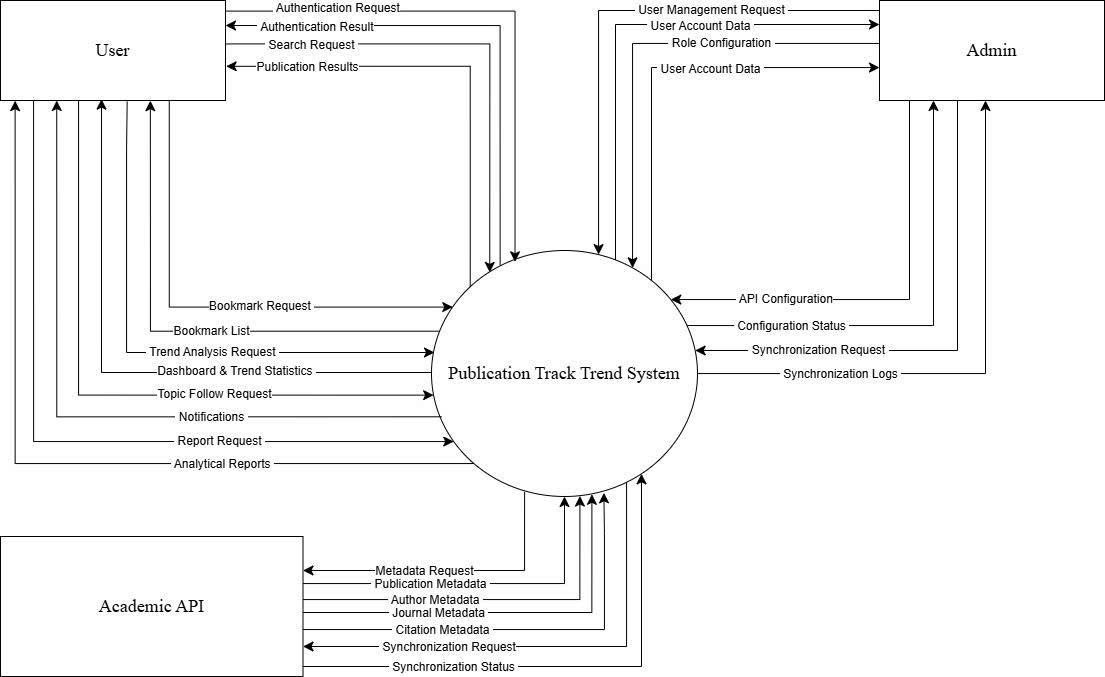
\includegraphics[width=0.95\textwidth]{Context_Diagram.png}

	\label{fig: usecase}
\end{figure}

\section{User Requirements}

\subsection{Actors}


\begin{longtable}{|c|p{4cm}|p{9cm}|}
	\hline
	\textbf{\#} & \textbf{Actor} & \textbf{Description} \\
	\hline
	\endfirsthead
	
	\hline
	\textbf{\#} & \textbf{Actor} & \textbf{Description} \\
	\hline
	\endhead
	
	1 & User &
	System user who can search scientific publications, view publication details, save bookmarks, follow research topics, receive notifications, and analyze publication trends. \\
	\hline
	
	2 & Administrator &
	System administrator responsible for managing users, configuring the system, setting up and validating academic data sources (OpenAlex, Crossref,Semantic Scholar API), synchronizing data, and monitoring system operations. \\
	\hline
	
	3 & Publication Trend Tracking System &
	The core system that handles all functionalities such as paper search, trend analysis, dashboard generation, trending topic detection, bookmark management, notification delivery, and report generation. \\
	\hline
	
	4 & Academic API &
	External services such as OpenAlex and Crossref that provide scientific publication metadata (authors, journals, citations) for system synchronization and analysis. \\
	\hline
	
\end{longtable}

\clearpage


\subsection{Use Case Diagrams}
\subsubsection{Diagram}
\begin{figure}[H]
	\centering
	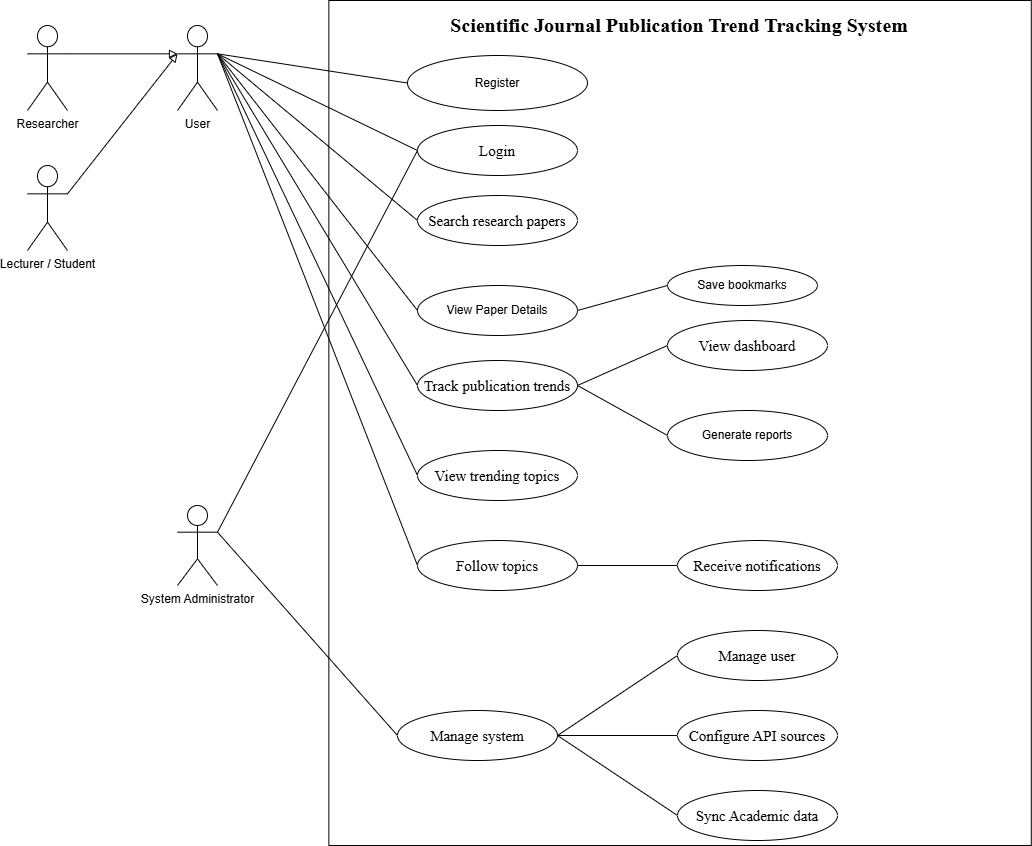
\includegraphics[width=\textwidth]{ucd.png}
	\caption{Use Case Diagram}
	\label{fig:usecase}
\end{figure}

\subsubsection{Use Case Descriptions}
\small
% Đặt 2 dòng định nghĩa màu này TRƯỚC bảng (chỉ cần định nghĩa 1 lần trong toàn bộ file,
% nếu đã có \definecolor{mintheader} / \definecolor{mintrow} ở chỗ khác rồi thì bỏ qua 2 dòng dưới)
\definecolor{mintheader}{HTML}{7DCEA0}
\definecolor{mintrow}{HTML}{EAFBF1}

\begin{longtable}{|>{\raggedright\arraybackslash}p{2cm}|>{\raggedright\arraybackslash}p{1.8cm}|>{\raggedright\arraybackslash}p{2.7cm}|>{\raggedright\arraybackslash}p{4.7cm}|>{\raggedright\arraybackslash}p{2.8cm}|}
	\hline
	\rowcolor{mintheader}
	\textbf{Main UC Group} &
	\textbf{Main Agent (Actor)} &
	\textbf{Sub-UCs} &
	\textbf{Brief Description of the Process} &
	\textbf{Output} \\
	\hline
	\endfirsthead
	
	\hline
	\rowcolor{mintheader}
	\textbf{Main UC Group} &
	\textbf{Main Agent (Actor)} &
	\textbf{Sub-UCs} &
	\textbf{Brief Description of the Process} &
	\textbf{Output} \\
	\hline
	\endhead
	
	\rowcolor{mintrow}
	Manage Account &
	User &
	Register, Login &
	Users create an account and authenticate to access the Scientific Journal Publication Trend Tracking System. &
	A registered account is created and a secure user session is established. \\
	\hline
	
	\rowcolor{mintrow}
	Search Publications &
	User &
	Search Research Papers, View Paper Details &
	Users search scientific publications using keywords, author names, or journal names and view detailed publication metadata. &
	Matching publications and detailed publication information are displayed. \\
	\hline
	
	\rowcolor{mintrow}
	Manage Bookmarks &
	User &
	Save Bookmarks &
	Users save selected publications into their personal bookmark collection for future reference. &
	The selected publication is stored in the user's bookmark list. \\
	\hline
	
	\rowcolor{mintrow}
	Track Publication Trends &
	User &
	Track Publication Trends, View Dashboard, View Trending Topics &
	Users analyze publication trends by keyword, topic, author, journal, and time range. The system generates statistical charts and identifies trending research topics. &
	Trend statistics, dashboards and trending topics are displayed. \\
	\hline
	
	\rowcolor{mintrow}
	Follow Topics &
	User &
	Follow Topics, Receive Notifications &
	Users follow research topics to receive notifications about tracked activities &
	The selected topic is added to the user's followed-topic list and notifications become available. \\
	\hline
	
	\rowcolor{mintrow}
	Generate Reports &
	User &
	Generate Reports &
	Users generate analytical reports based on publication trend analysis and selected report parameters. &
	An analytical report summarizing publication trends is generated. \\
	\hline
	
	\rowcolor{mintrow}
	Manage System &
	Administrator &
	Manage System, Configure API Sources, Synchronize Academic Data &
	Administrators manage system settings, configure academic APIs, synchronize publication metadata and maintain system operations. &
	System settings and publication metadata are successfully updated. \\
	\hline
	
	\rowcolor{mintrow}
	Manage Users &
	Administrator &
	Manage Users &
	Administrators manage user accounts, roles, permissions and account status. &
	User information and access permissions are updated. \\
	\hline
	
	\rowcolor{mintrow}
	Configure API Sources &
	Administrator &
	Configure API Sources &
	Administrators configure, update and test external academic APIs such as OpenAlex, Crossref and Semantic Scholar. &
	API configuration settings are successfully validated and stored. \\
	\hline
	
	\rowcolor{mintrow}
	Synchronize Academic Data &
	Administrator &
	Synchronize Academic Data &
	Administrators synchronize publication metadata from external academic APIs into the local database for searching and trend analysis. &
	The publication metadata database is updated with the latest synchronized records. \\
	\hline
	
\end{longtable}
\section{Functional Requirement}
\subsection{System Functional Overview}
\subsubsection{Screens Flow}


\begin{figure}[H]
	\centering
	
\includegraphics[width=\textwidth]{res.jpg}

	\label{fig:Screen Description-view-paper-details}
\end{figure}
\begin{figure}[H]
	\centering
	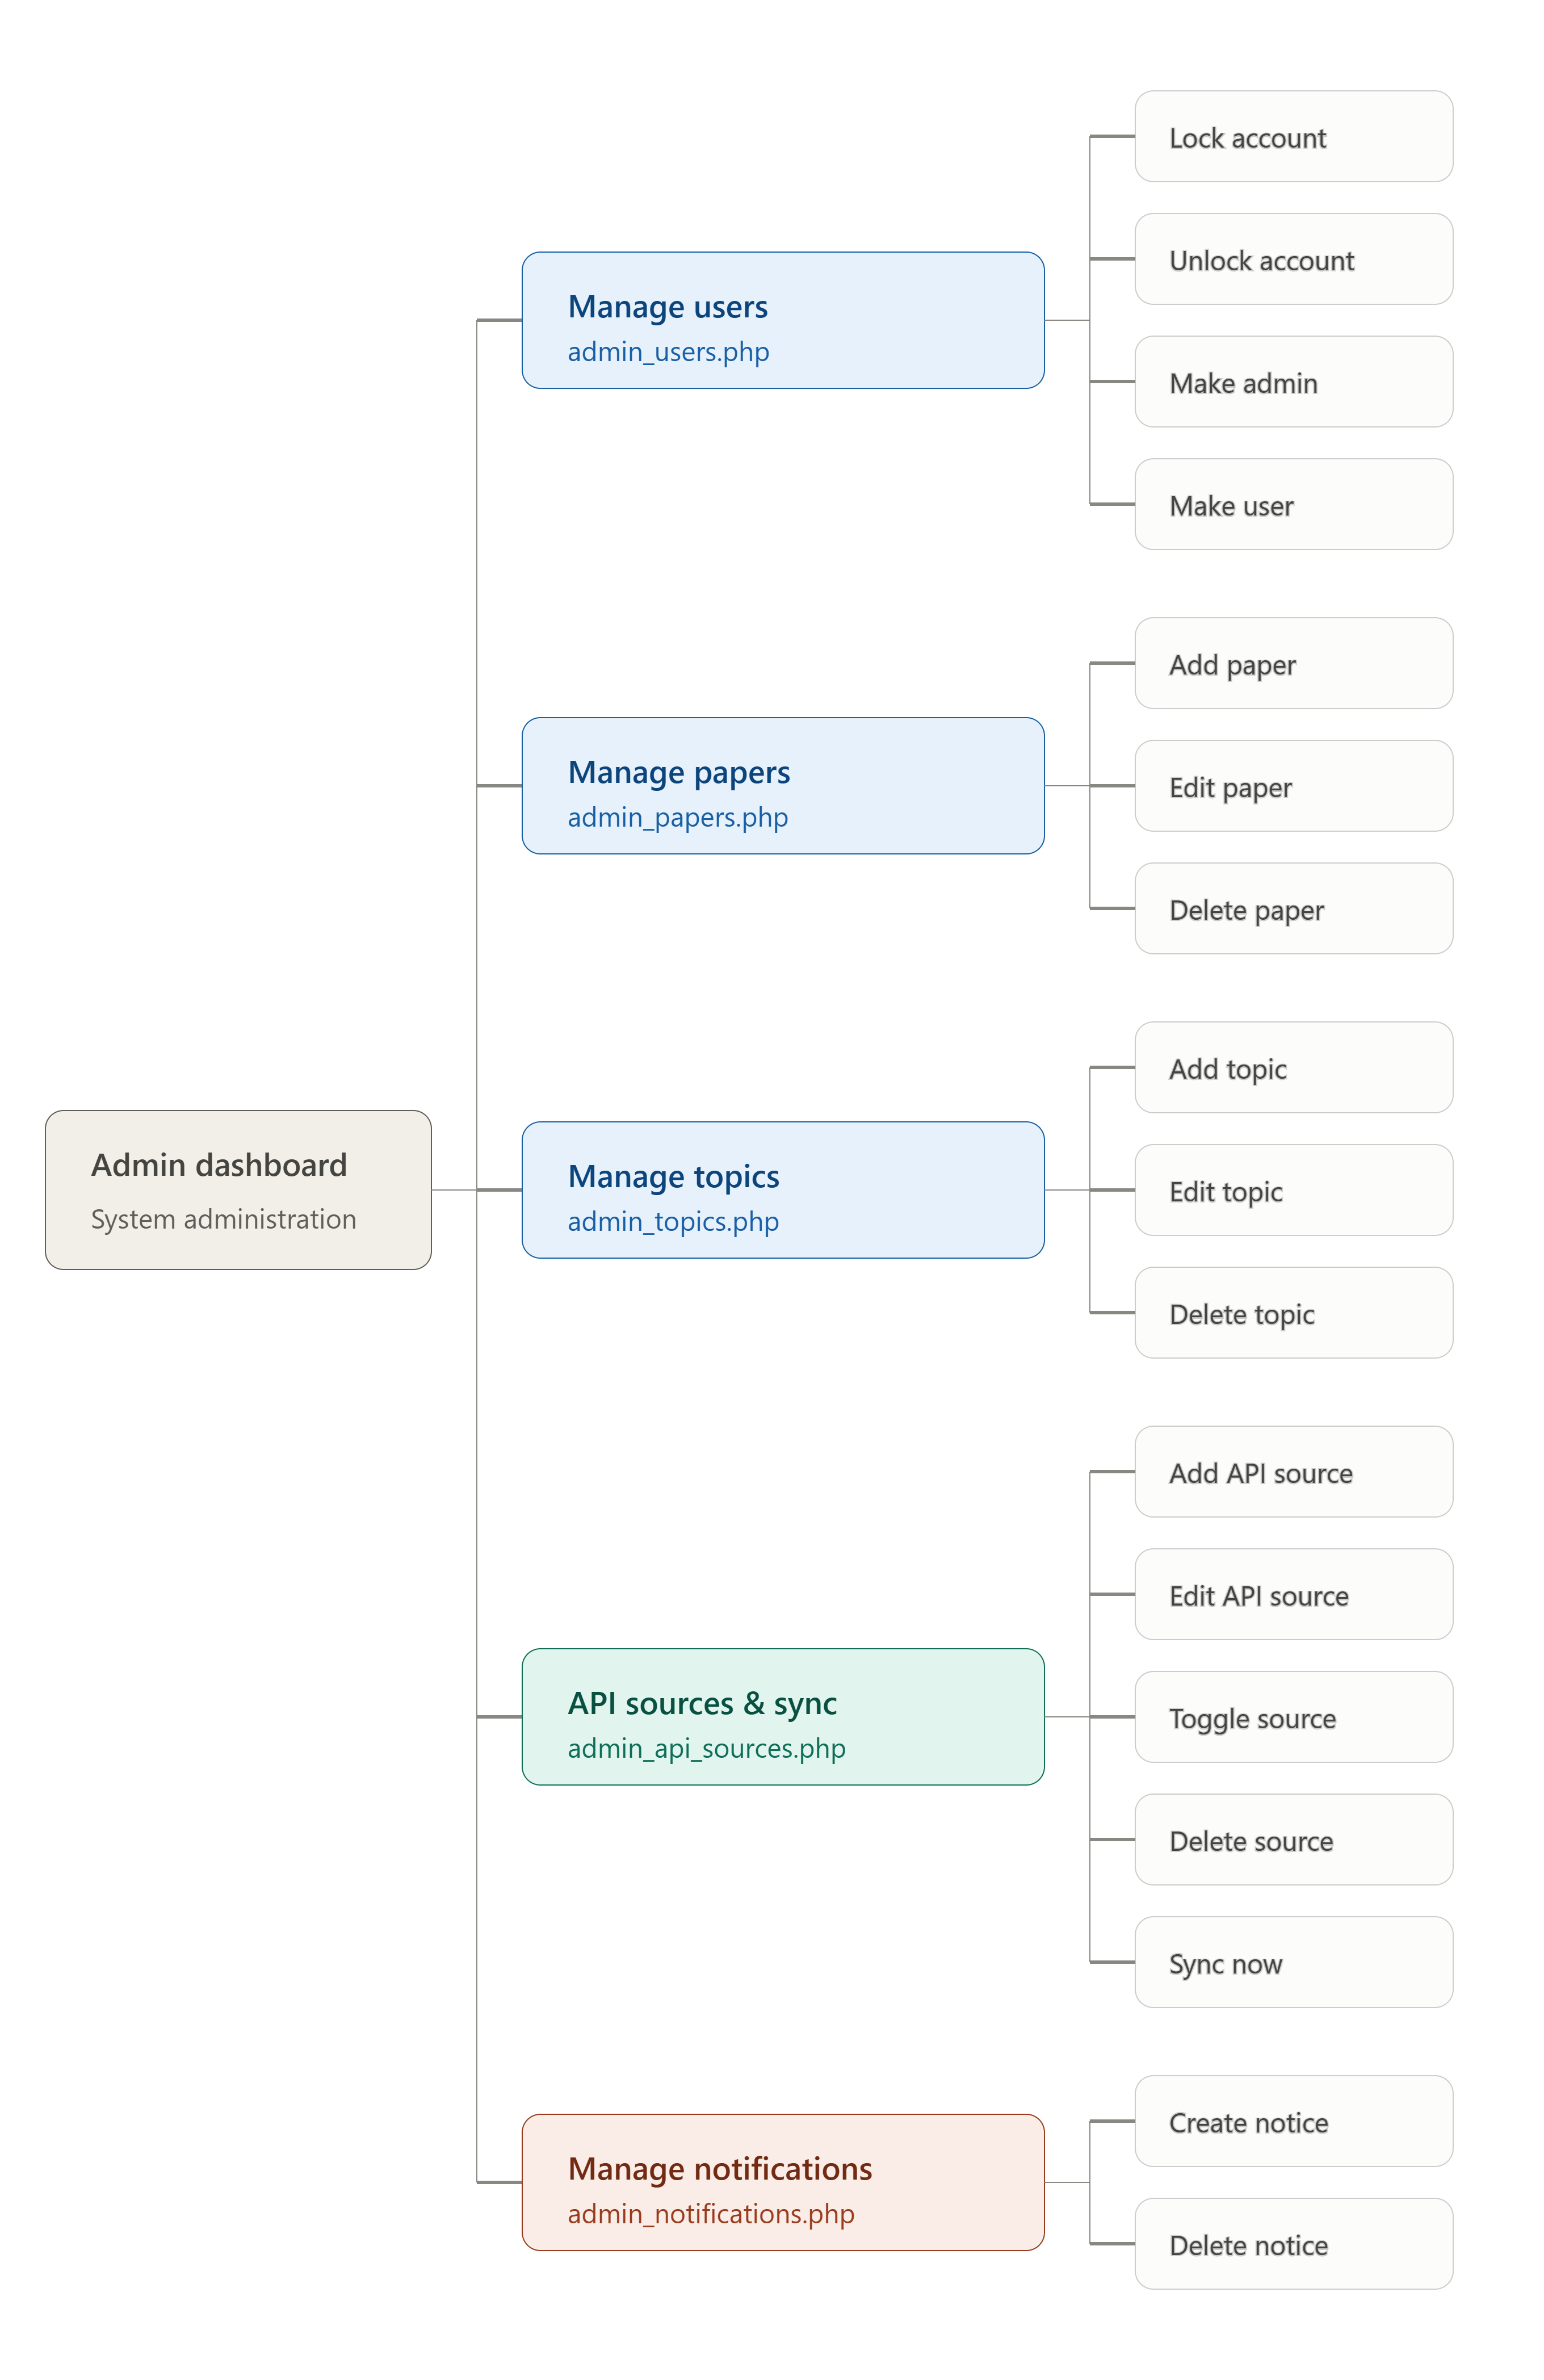
\includegraphics[width=\textwidth]{admin.png}

	\label{fig:Screen Description-view-paper-details}
\end{figure}


% ========================================================================
% PHẦN NÀY CHỈ CHỨA BẢNG - dán vào vị trí bạn muốn trong báo cáo đã có
% Các package bên dưới cần thêm vào PHẦN PREAMBLE (trước \begin{document})
	% của báo cáo gốc, KHÔNG dán \documentclass hay \usepackage vào giữa văn bản
	% ------------------------------------------------------------------------
	% \usepackage{array}
	% \usepackage{longtable}
	% \usepackage{amsmath}
	% \usepackage{booktabs}
	% \usepackage[table]{xcolor}
	% ========================================================================
	
	\renewcommand{\arraystretch}{1.3}
	\rowcolors{2}{gray!8}{white}
	
	\begin{longtable}{|>{\raggedright\arraybackslash}p{0.15\textwidth}|>{\raggedright\arraybackslash}p{0.20\textwidth}|>{\raggedright\arraybackslash}p{0.57\textwidth}|}
		\toprule
		\rowcolor{gray!25}
		Functional Group &
		Screen Name &
		Detailed Description \\
		\midrule
		\endfirsthead
		
		\toprule
		\rowcolor{gray!25}
		Functional Group &
		Screen Name &
		Detailed Description \\
		\midrule
		\endhead
		
		\bottomrule
		\endfoot
		
		\bottomrule
		\endlastfoot
		
		User Authentication &
		Login &
		Purpose: Allows users to log into the system. Components: Username, Password, Login button, and Register link. Flow: The user enters credentials $\rightarrow$ The system authenticates the user $\rightarrow$ The main system interface is displayed. Rule: Username and password are required; invalid credentials will generate an error message. \\
		
		User Authentication &
		Register &
		Purpose: Allows new users to create an account. Components: Full Name, Email, Username, Password, and Register button. Flow: The user enters the required information $\rightarrow$ The system validates the email and username $\rightarrow$ A new account is created $\rightarrow$ The user is redirected to the Login page. Rules: Email and username must be unique; passwords are securely hashed before storage. \\
		
		Paper Management &
		Search Research Papers &
		Purpose: Allows users to search scientific publications by keyword, author, or journal. Components: Search box, filters, Search button, and result list. Flow: The user enters search criteria $\rightarrow$ The system searches publication metadata $\rightarrow$ Matching publications are displayed. \\
		
		Paper Management &
		View Paper Details &
		Purpose: Displays detailed metadata of a selected research paper. Components: Title, Authors, Abstract, Keywords, Publication Year, Journal Name, Citation Information, and Save Bookmark button. Flow: The user selects a paper $\rightarrow$ The system retrieves publication metadata $\rightarrow$ Paper details are displayed. \\
		
		Paper Management &
		Bookmarks &
		Purpose: Manages the user's bookmarked papers. Components: Bookmark list, Delete Bookmark button. Flow: The user views or removes bookmarked papers. Rule: Duplicate bookmarks are not allowed. \\
		
		Publication Trend Analysis &
		Track Publication Trends &
		Purpose: Analyzes publication trends based on keywords, research topics, authors, or journals. Components: Search filters, time range selector, and Analyze button. Flow: The user enters analysis criteria $\rightarrow$ The system analyzes publication metadata $\rightarrow$ Statistical results and charts are displayed. \\
		
		Publication Trend Analysis &
		Dashboard &
		Purpose: Displays an overview of publication statistics. Components: Publications by year chart, Topic distribution chart, Journal distribution chart, and Growth trend chart. Flow: The system generates dashboard visualizations after trend analysis is completed. \\
		
		Publication Trend Analysis &
		Trending Topics &
		Purpose: Displays the most popular research topics. Flow: The system analyzes publication data $\rightarrow$ Ranks research topics $\rightarrow$ Displays trending topics. \\
		
		Topic Management &
		Follow Topics &
		Purpose: Allows users to follow research topics of interest. Components: Topic list and Follow button. Flow: The user selects a topic $\rightarrow$ The system stores it in the followed-topic list. \\
		
		Notifications &
		Notifications &
		Purpose: Displays system notifications or notifications when following a new topic. Flow: The system generates notifications $\rightarrow$ The user views notification details and marks them as read. \\
		
		Reporting &
		Generate Reports &
		Purpose: Generates reports based on publication trend analysis. Flow: The user clicks "Generate Report" $\rightarrow$ The system displays options: Preview \& Print / Save as PDF, Direct PDF Download, and Download Report (HTML) $\rightarrow$ The system executes the request based on the selected option and completes the generation, display, or export of the analytical report. \\
		
		System Administration &
		Manage System &
		Purpose: Provides administrative functions for system management. Components: User Management, API Configuration, and Academic Data Synchronization. Flow: The administrator selects a management function $\rightarrow$ The system performs the requested operation. \\
		
		System Administration &
		Manage Users &
		Purpose: Manages user accounts. Components: User list, Change User Role, Activate Account, and Deactivate Account. Flow: The administrator selects a user $\rightarrow$ Updates account information $\rightarrow$ Saves the changes. \\
		
		System Administration &
		Configure API Sources &
		Purpose: To define and manage external academic data sources. Flow: The administrator enters source details (Name, URL, Priority, Status, Description). The administrator clicks "Add API Source" to save it to the system. The system displays the list, allowing the administrator to track, edit, or delete entries via the "Action" column. \\
		
		System Administration &
		Synchronize Academic Data &
		Purpose: Synchronize publication data from external APIs into the system. Components: API List, Synchronize button, Synchronization Log. Workflow: Click Synchronize $\rightarrow$ The system retrieves data from the APIs $\rightarrow$ Updates the database $\rightarrow$ Displays the synchronization result. \\
		
	\end{longtable}
\subsubsection{Screen Authorization}

{
	\newcolumntype{L}[1]{>{\raggedright\arraybackslash}p{#1}}
	\newcolumntype{C}[1]{>{\centering\arraybackslash}p{#1}}
	\renewcommand{\arraystretch}{1.6}
	\setlength{\tabcolsep}{6pt}
	
	
	\vspace{6pt}
	
\newcolumntype{L}[1]{>{\raggedright\arraybackslash}p{#1}}
\newcolumntype{C}[1]{>{\centering\arraybackslash}p{#1}}

\begin{longtable}{L{5.5cm} C{2.8cm} C{3.2cm} C{3.5cm}}
	\rowcolor{headerblue}
	\textcolor{white}{\textbf{Screen}} & \textcolor{white}{\textbf{Researcher}} & \textcolor{white}{\textbf{Lecturer/Student}} & \textcolor{white}{\textbf{System Administrator}} \\
	\hline
	\endfirsthead
	
	\rowcolor{headerblue}
	\textcolor{white}{\textbf{Screen}} & \textcolor{white}{\textbf{Researcher}} & \textcolor{white}{\textbf{Lecturer/Student}} & \textcolor{white}{\textbf{System Administrator}} \\
	\hline
	\endhead
	
	\hline
	\endfoot
	
	\rowcolor{rowblue} Login & x & x & x \\
	Logout & x & x & x \\
	\rowcolor{rowblue} Register & x & x & \\
	Search Research Papers & x & x & \\
	\rowcolor{rowblue} View Paper Details & x & x & \\
	Save Bookmarks & x & x & \\
	\rowcolor{rowblue} Track Publication Trends & x & x & \\
	View Dashboard & x & x & \\
	\rowcolor{rowblue} Generate Reports & x & x & \\
	View Trending Topics & x & x & \\
	\rowcolor{rowblue} Follow Topics & x & x & \\
	Receive Notifications & x & x & \\
	\rowcolor{rowblue} View Profile & x & x & \\
	Edit Profile & x & x & \\
	\rowcolor{rowblue} View Notifications & x & x & \\
	Create Report & x & x & \\
	\rowcolor{rowblue} Manage System & & & x \\
	Manage Users & & & x \\
	\rowcolor{rowblue} Configure API Sources & & & x \\
	Sync Academic Data & & & x \\
	
\end{longtable}
\subsubsection{Non-Screen Functions}

{
	\newcolumntype{L}[1]{>{\raggedright\arraybackslash}p{#1}}
	\newcolumntype{C}[1]{>{\centering\arraybackslash}p{#1}}
	\renewcommand{\arraystretch}{1.6}
	\setlength{\tabcolsep}{6pt}
	

	
	\vspace{6pt}
	
\begin{tabular}{C{0.8cm} L{3.5cm} C{2.5cm} L{7cm}}
	
	\rowcolor{headerblue}
	{\color{white}\bfseries \#} &
	{\color{white}\bfseries Feature} &
	{\color{white}\bfseries System Function} &
	{\color{white}\bfseries Description} \\
	
	\rowcolor{rowblue}
	1 & Automated Academic Data Synchronization & Scheduled Job &
	Scheduled job that automatically retrieves publication metadata directly from external academic APIs (OpenAlex and Crossref). The retrieved data is used for publication search, statistical analysis, and publication trend tracking. \\
	
	\rowcolor{rowwhite}
	2 & Automated Trend Calculation & Scheduled Job &
	Scheduled job that automatically recalculates publication trend statistics after each data synchronization from external academic APIs. The system analyzes total publications, total citations, Open Access rate, and research topic trends, then updates the data displayed on the dashboard and Trending Topics. \\
	
\end{tabular}
}
\subsection{ Entity Relationship Diagram }
\begin{figure}[H]
	\centering
	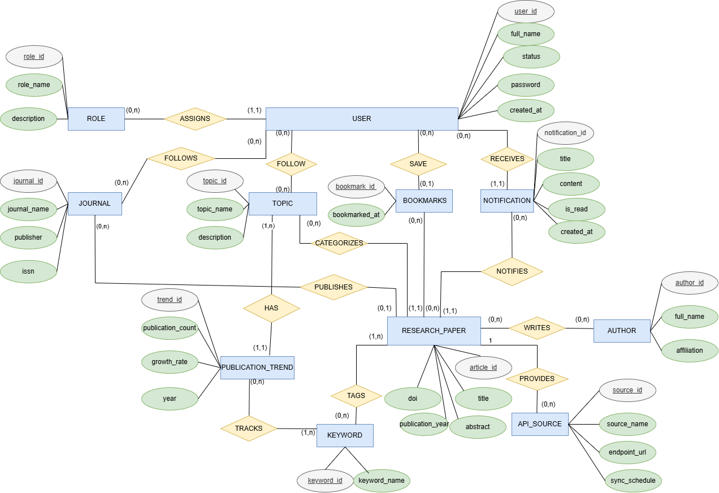
\includegraphics[width=\textwidth]{erd.png}

	\label{fig:erd}
\end{figure}
\subsection{Authentication}
\subsubsection{ Register }
\textbf{Role:} User \\
\textbf{Function trigger:} The user clicks Đăng kí. \\
\textbf{Function description:}
\begin{itemize}[label=-]
	\item Purpose: Create a new user account.
	\item Data processing: Validate user information and store it in the database.
\end{itemize}
\textbf{Function Details:}
\begin{itemize}[label=-]
	\item Whether the username , email already exists
	\item Validate password requirements.
	\item Create a new account.
	\item Display a success message.

\end{itemize}

\begin{figure}[H]
	\centering
	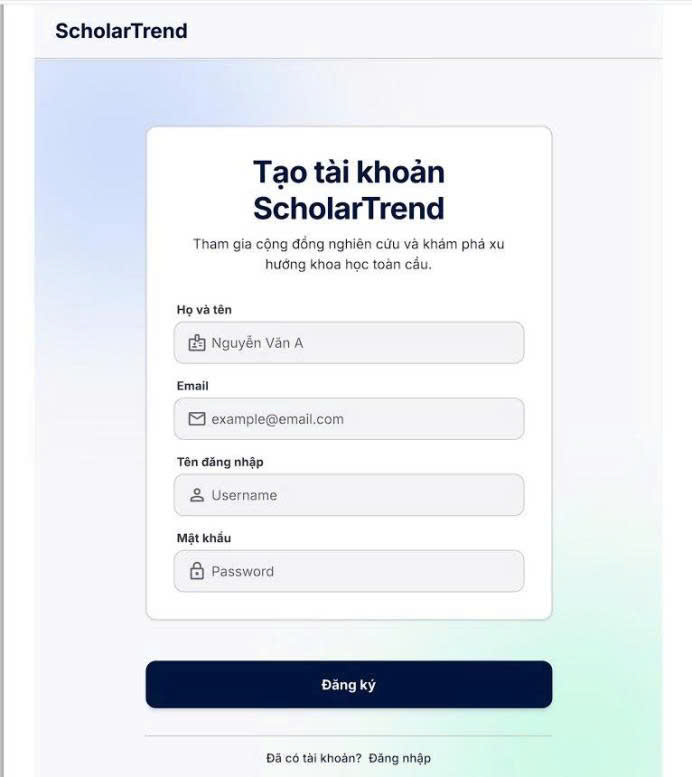
\includegraphics[width=\textwidth]{gđk.jpg}

	\label{fig:erd}
\end{figure}
\begin{itemize}[label=-]
	\item Email already exists
\end{itemize}
\begin{figure}[H]
	\centering
	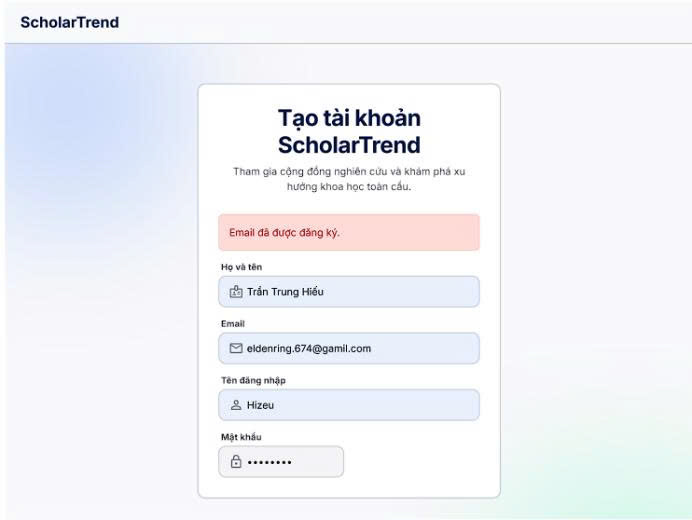
\includegraphics[width=\textwidth]{dkl.jpg}

	\label{fig:erd}
\end{figure}

\begin{itemize}[label=-]
	\item Username already exists.
\end{itemize}
\begin{figure}[H]
	\centering
	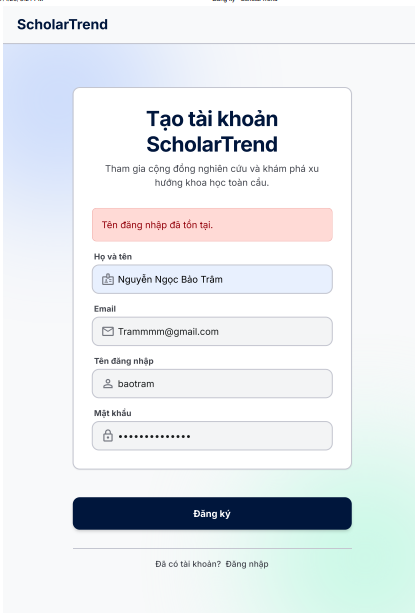
\includegraphics[width=\textwidth]{tentontai.png}

	\label{fig:erd}
\end{figure}
\begin{itemize}[label=-]
	\item Password does not meet the required format.
\end{itemize}

\begin{figure}[H]
	\centering
	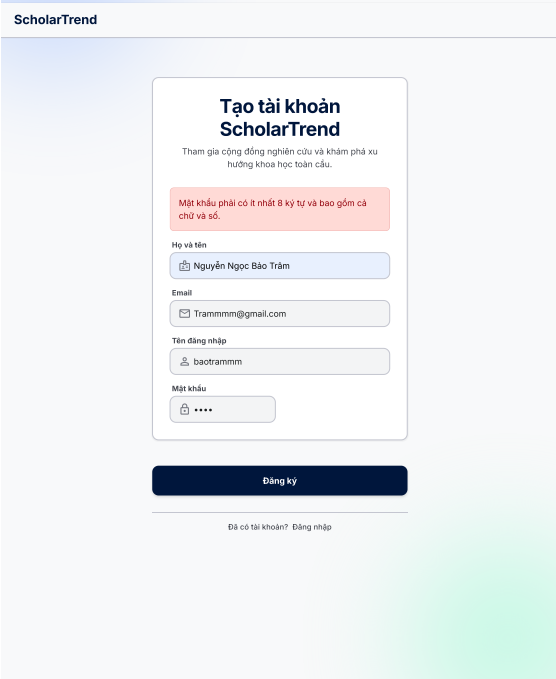
\includegraphics[width=\textwidth]{matkhaukhac.png}
	
	\label{fig:erd}
\end{figure}

\begin{itemize}[label=-]
	\item Registration successful.
\end{itemize}
\begin{figure}[H]
	\centering
	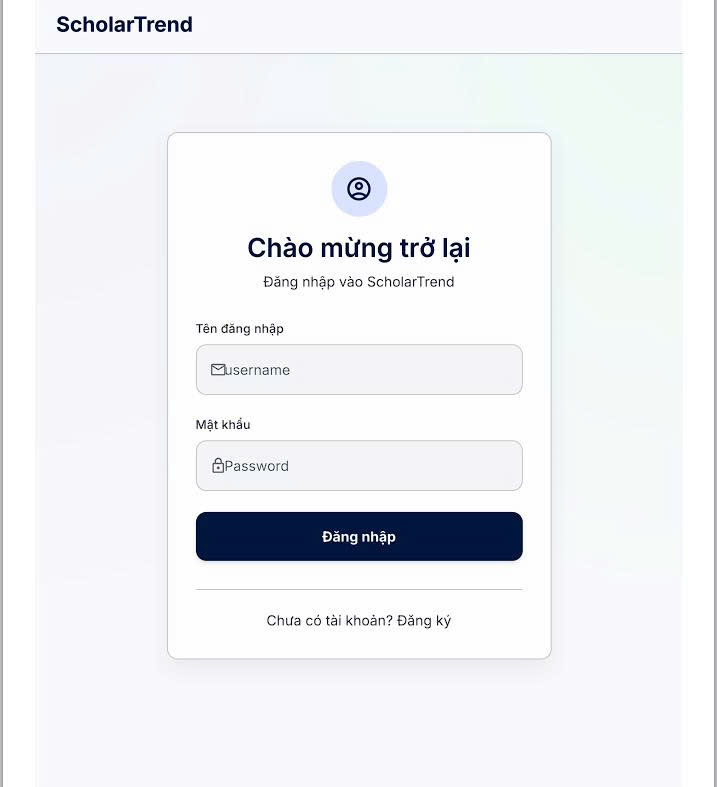
\includegraphics[width=\textwidth]{dk.jpg}
	\caption{Login Page}
	\label{fig:erd}
\end{figure}
\subsubsection{Login}


\textbf{Role:} User

\textbf{Function trigger:}

- The user enters a username and password to log in.

\textbf{Function description:}

- \textbf{Purpose:} Allow users to access the system.

- \textbf{Data processing:} Authenticate the entered username and password against the system database.

\textbf{Function Details:}

- If the login is successful, redirect the user to the Home page.

- If the login fails, display the error message: ``Tên đăng nhập hoặc mật khẩu không đúng.''
\begin{figure}[H]
\centering
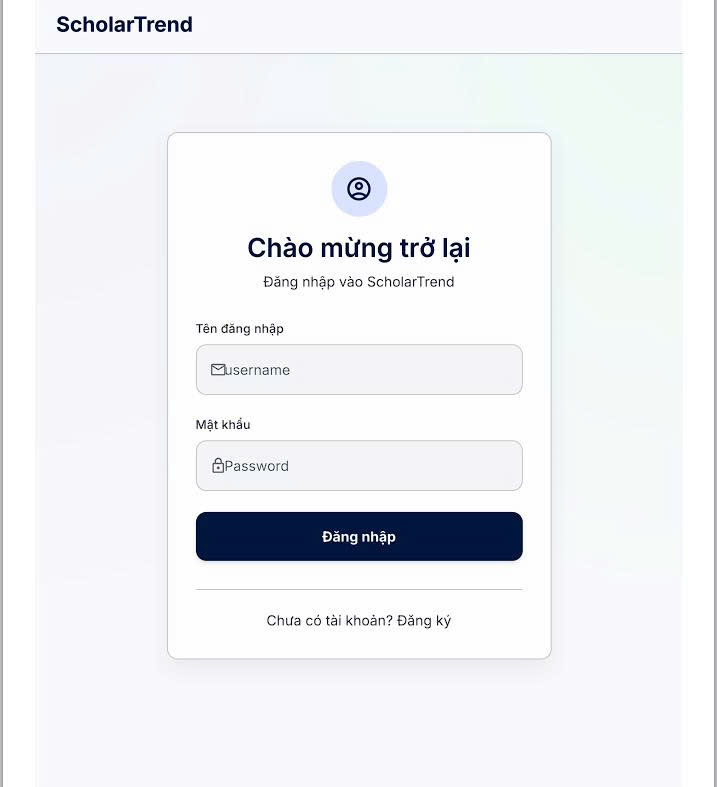
\includegraphics[width=\textwidth]{dk.jpg}

\label{fig:erd}
\end{figure}
\begin{itemize}[label=-]
	\item Invalid username or password.
\end{itemize}
\begin{figure}[H]
	\centering
	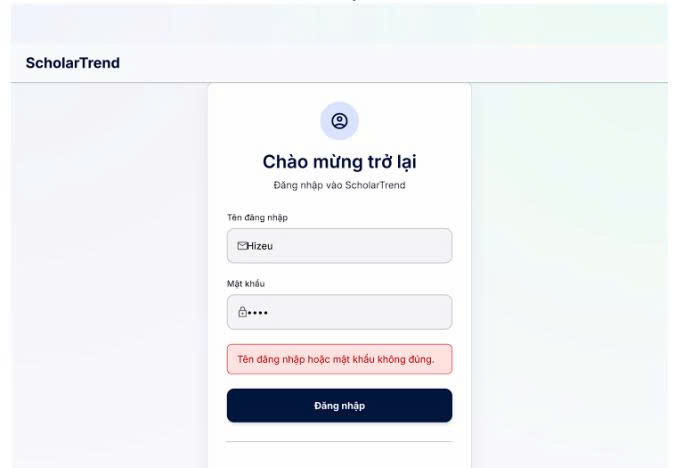
\includegraphics[width=\textwidth]{dnl.jpg}

	\label{fig:erd}
\end{figure}
\begin{itemize}[label=-]
	\item Login successful.
\end{itemize}
\begin{figure}[H]
	\centering
	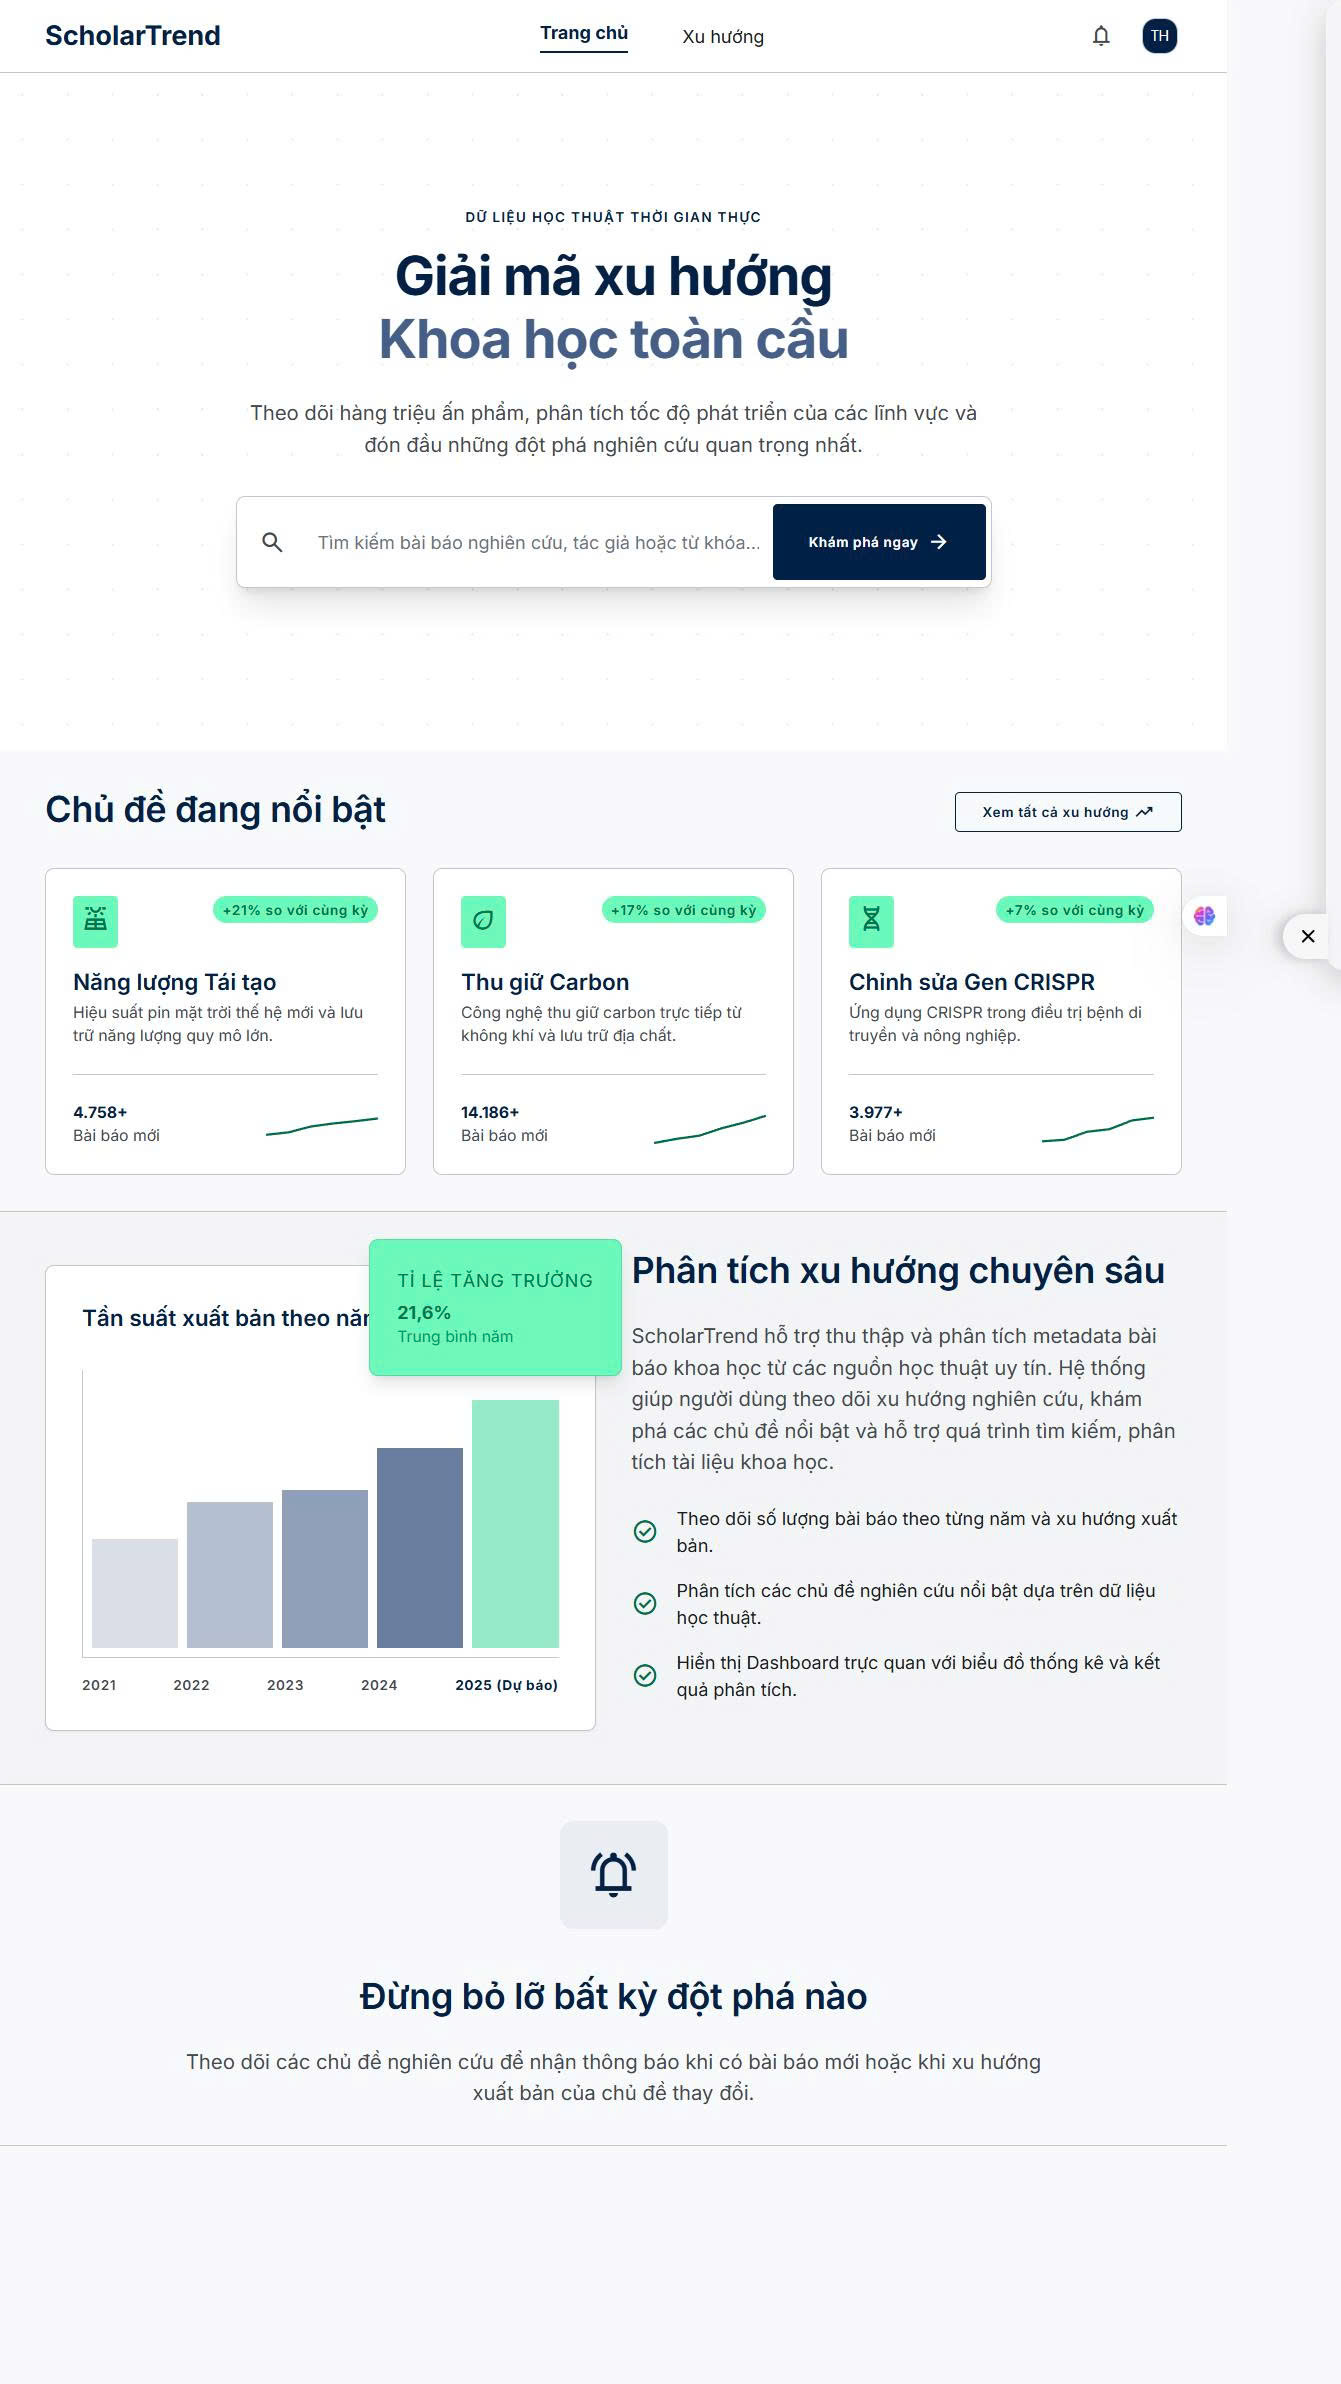
\includegraphics[width=\textwidth]{gdc.jpg}
	
	\label{fig:erd}
\end{figure}

\subsubsection{ Profile Management }

\textbf{Update Profile}

\textbf{Role:} User \\
\textbf{Function trigger:} The user opens the Profile page and clicks Chỉnh sửa thông tin. \\
\textbf{Function description:}
\begin{itemize}[label=-]
	\item Purpose: Allow users to update their personal information.
	\item Data processing: Validate and save the updated information.
\end{itemize}
\textbf{Function Details:}
\begin{itemize}[label=-]
	\item Update name, Email and other personal information.
	\item Display a success message after saving.
\end{itemize}
\begin{figure}[H]
	\centering
	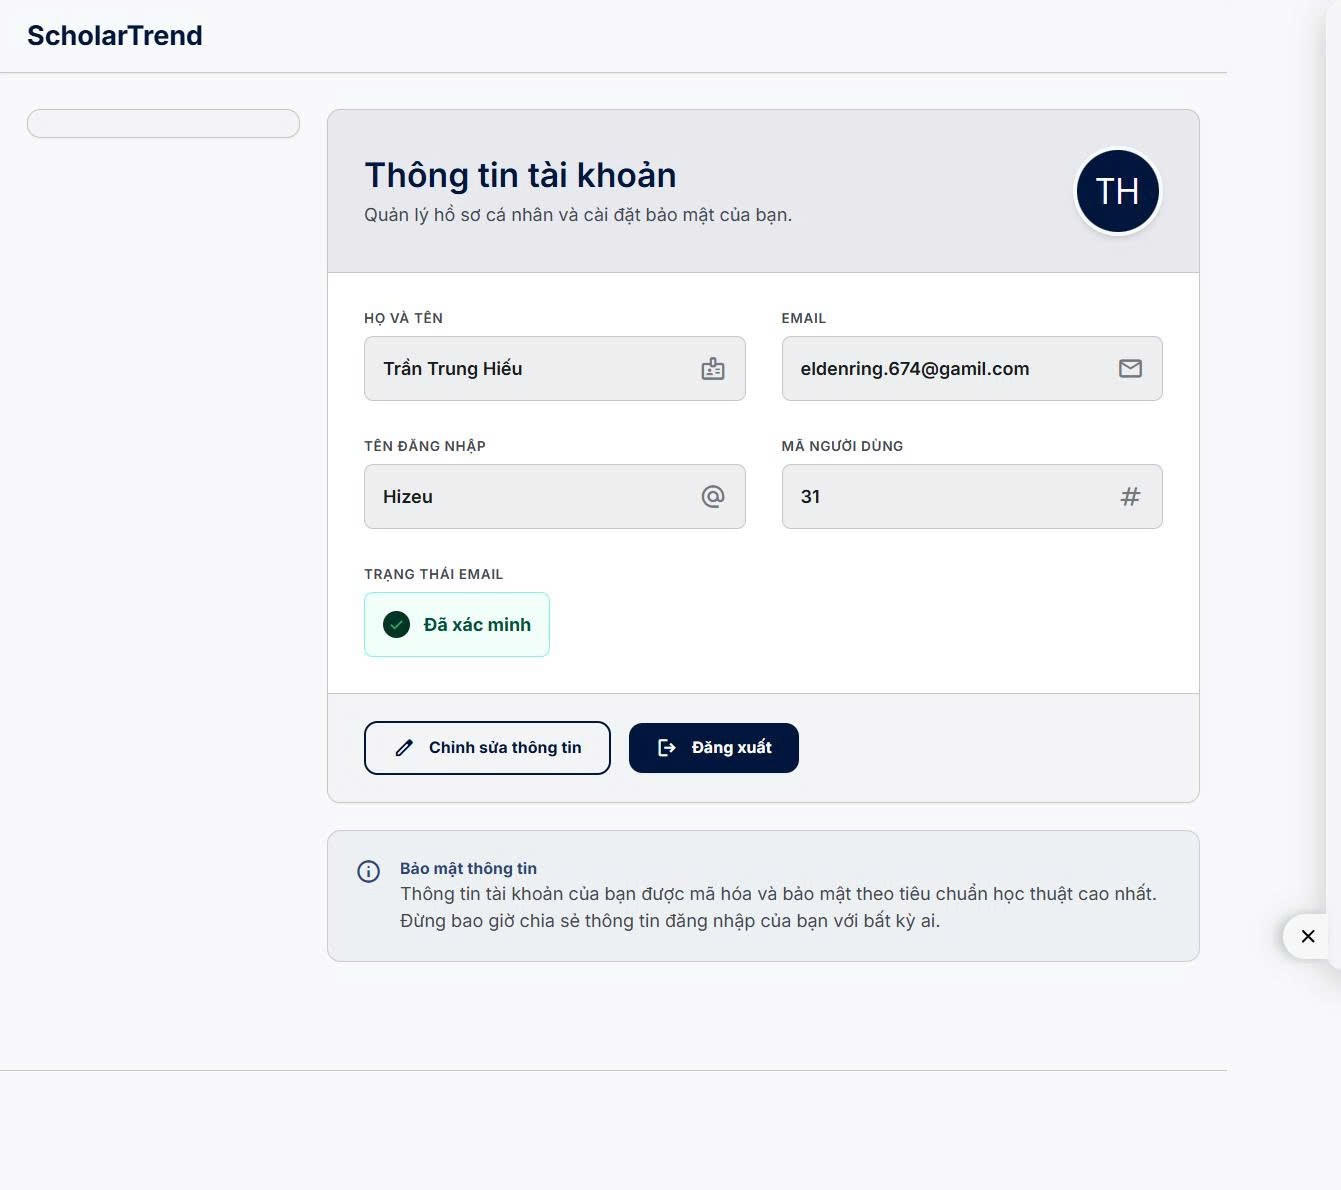
\includegraphics[width=\textwidth]{prof.jpg}

	\label{fig:erd}
\end{figure}
\begin{itemize}[label=-]
	\item Edit Profile
\end{itemize}
\begin{figure}[H]
	\centering
	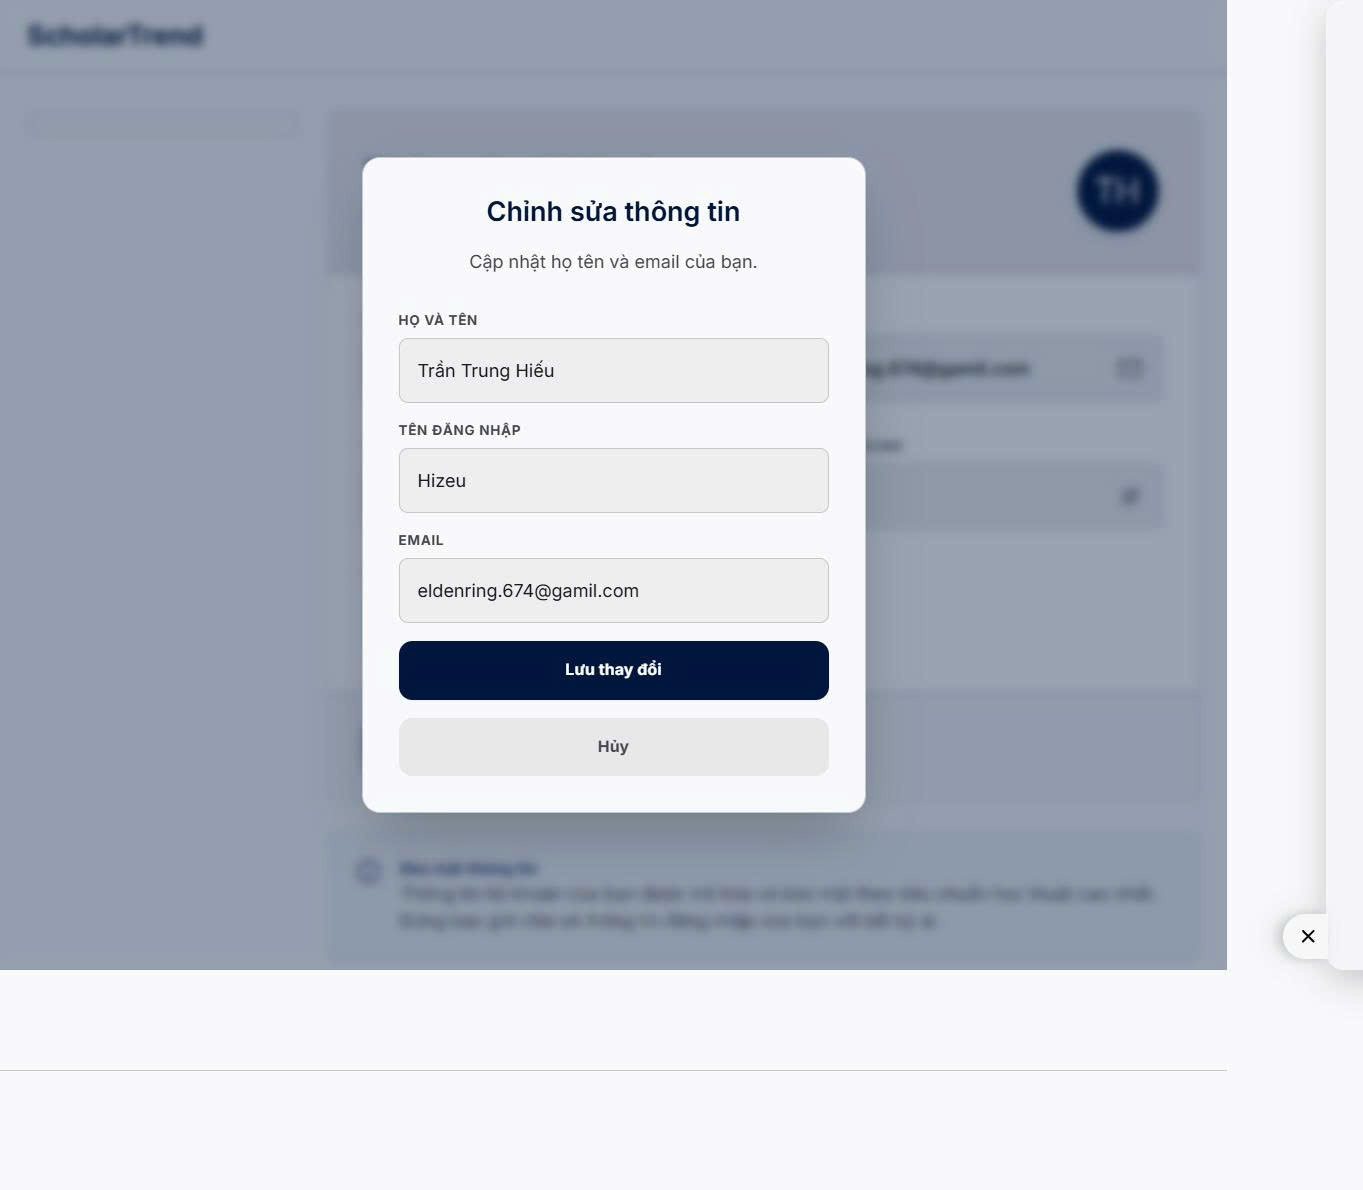
\includegraphics[width=\textwidth]{editprof.jpg}

	\label{fig:erd}
\end{figure}
\begin{itemize}[label=-]
	\item Username already exists.
\end{itemize}
\begin{figure}[H]
	\centering
	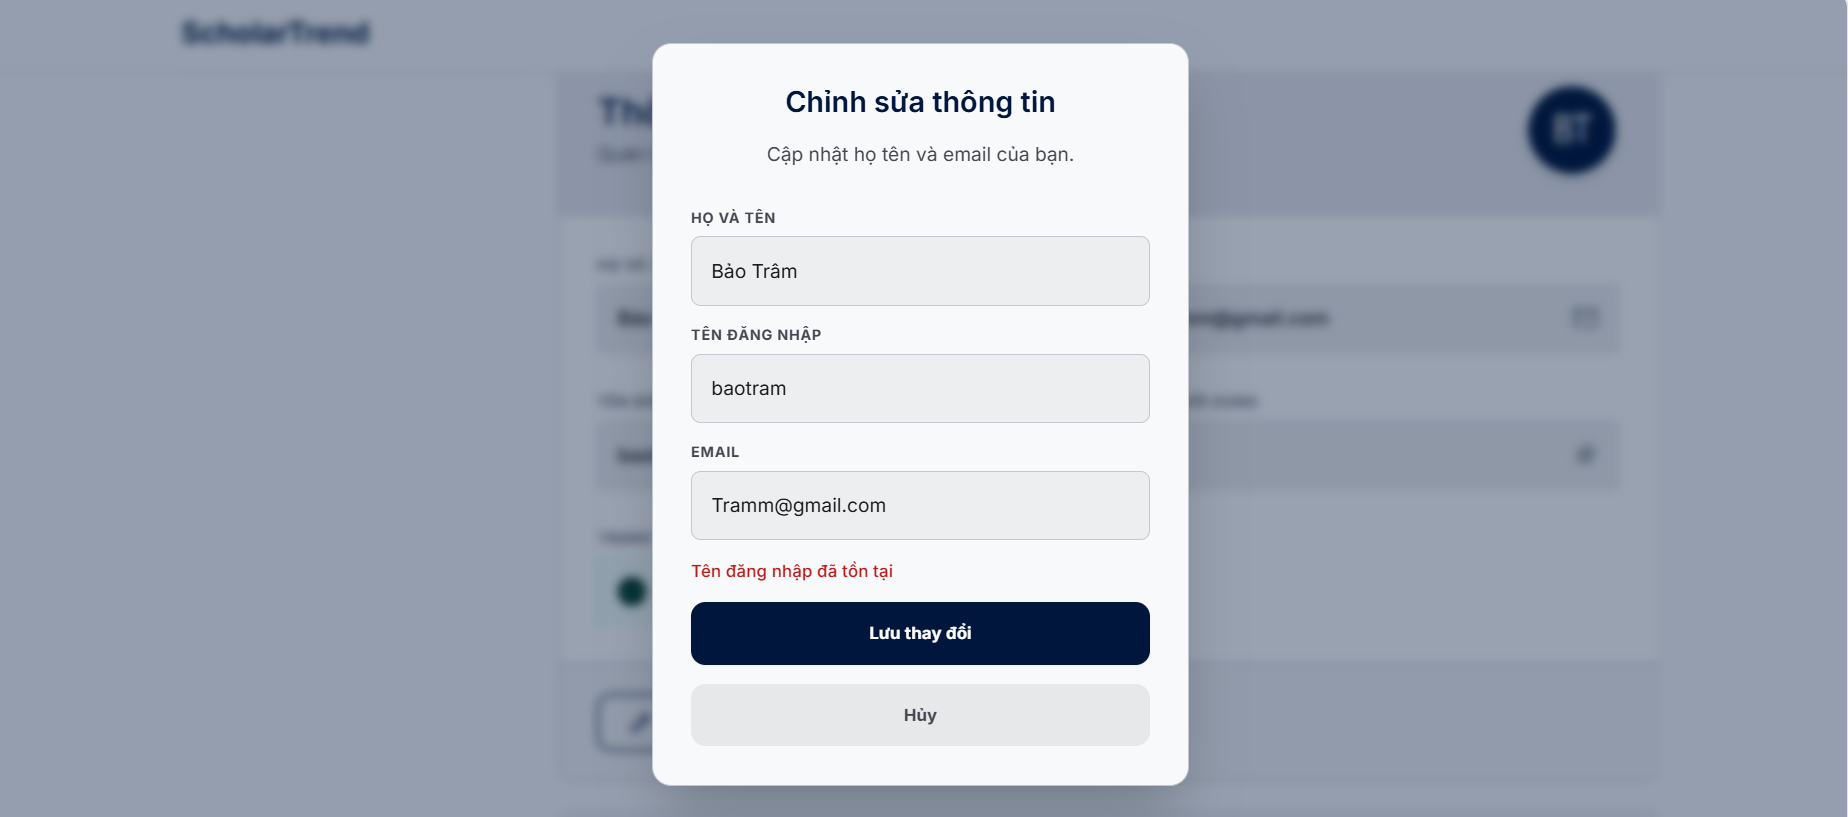
\includegraphics[width=\textwidth]{tencstontai.png}

	\label{fig:erd}
\end{figure}
\begin{itemize}[label=-]
	\item Invalid email address
\end{itemize}
\begin{figure}[H]
	\centering
	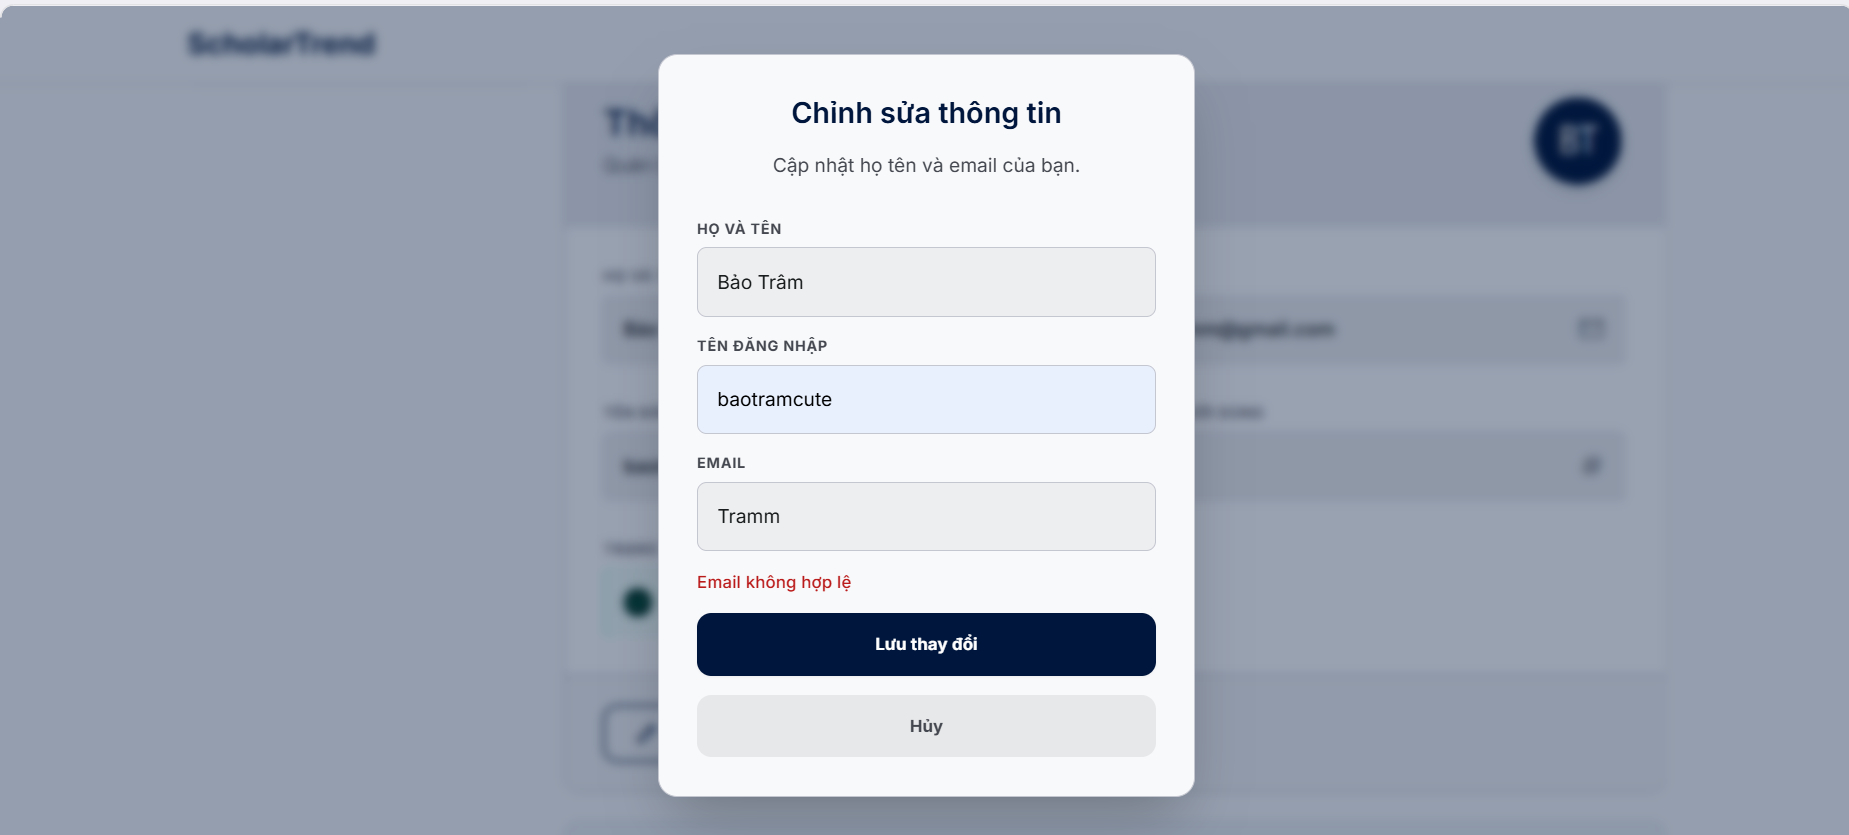
\includegraphics[width=\textwidth]{emailkhonghople.png}

	\label{fig:erd}
\end{figure}
\begin{itemize}[label=-]
	\item Update successful.
\end{itemize}
\begin{figure}[H]
	\centering
	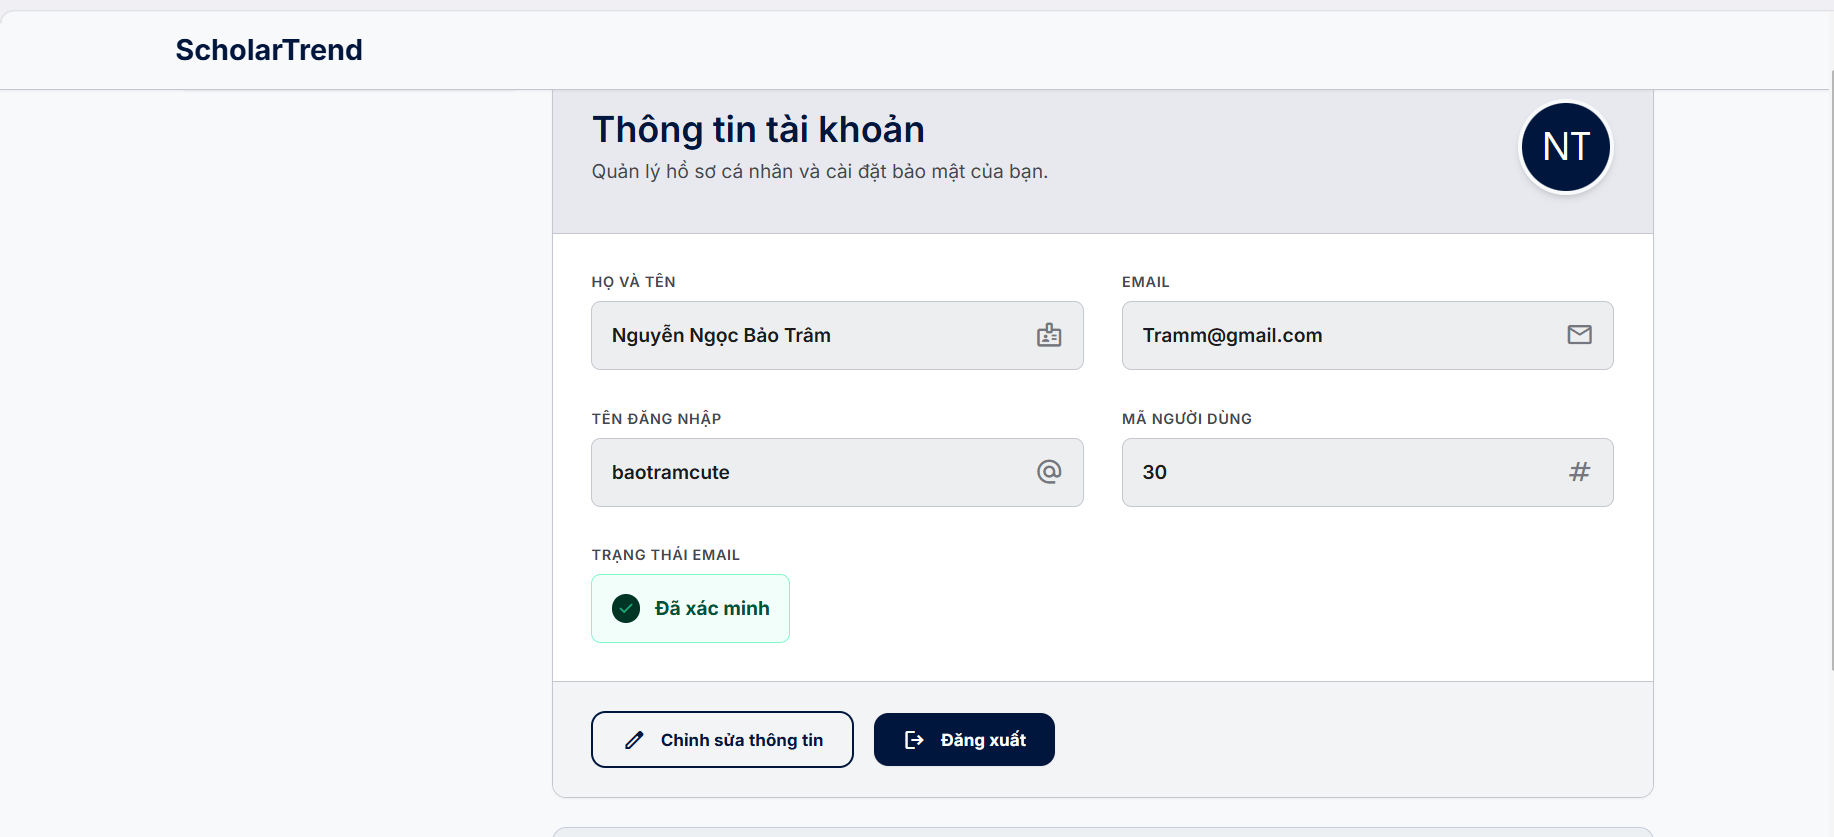
\includegraphics[width=\textwidth]{chinhsuathanhcong.png}

	\label{fig:erd}
\end{figure}
\subsubsection{ Logout }

\textbf{Role:} User \\
\textbf{Function trigger:} The user opens the Profile page and clicks Đăng xuất. \\
\textbf{Function description:}
\begin{itemize}[label=-]
	\item Purpose: Allow the user to securely log out of the system.
	\item Data processing: End the current user session.
\end{itemize}
\textbf{Function Details:}
\begin{itemize}[label=-]
	\item Display a confirmation dialog asking whether the user wants to Đăng xuất.
	\item If the user selects Đăng xuất, the system logs the user out and redirects them to the Đăng nhập page.
	\item If the user selects Hủy, the dialog is closed and the user remains on the current page.
\end{itemize}
\begin{figure}[H]
	\centering
	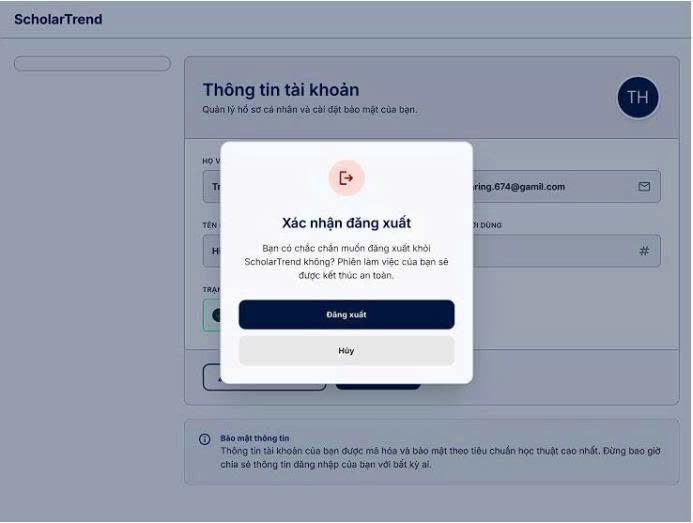
\includegraphics[width=\textwidth]{logout.jpg}

	\label{fig:erd}
\end{figure}
\begin{itemize}[label=-]
	\item Signed out successfully.
\end{itemize}
\begin{figure}[H]
	\centering
	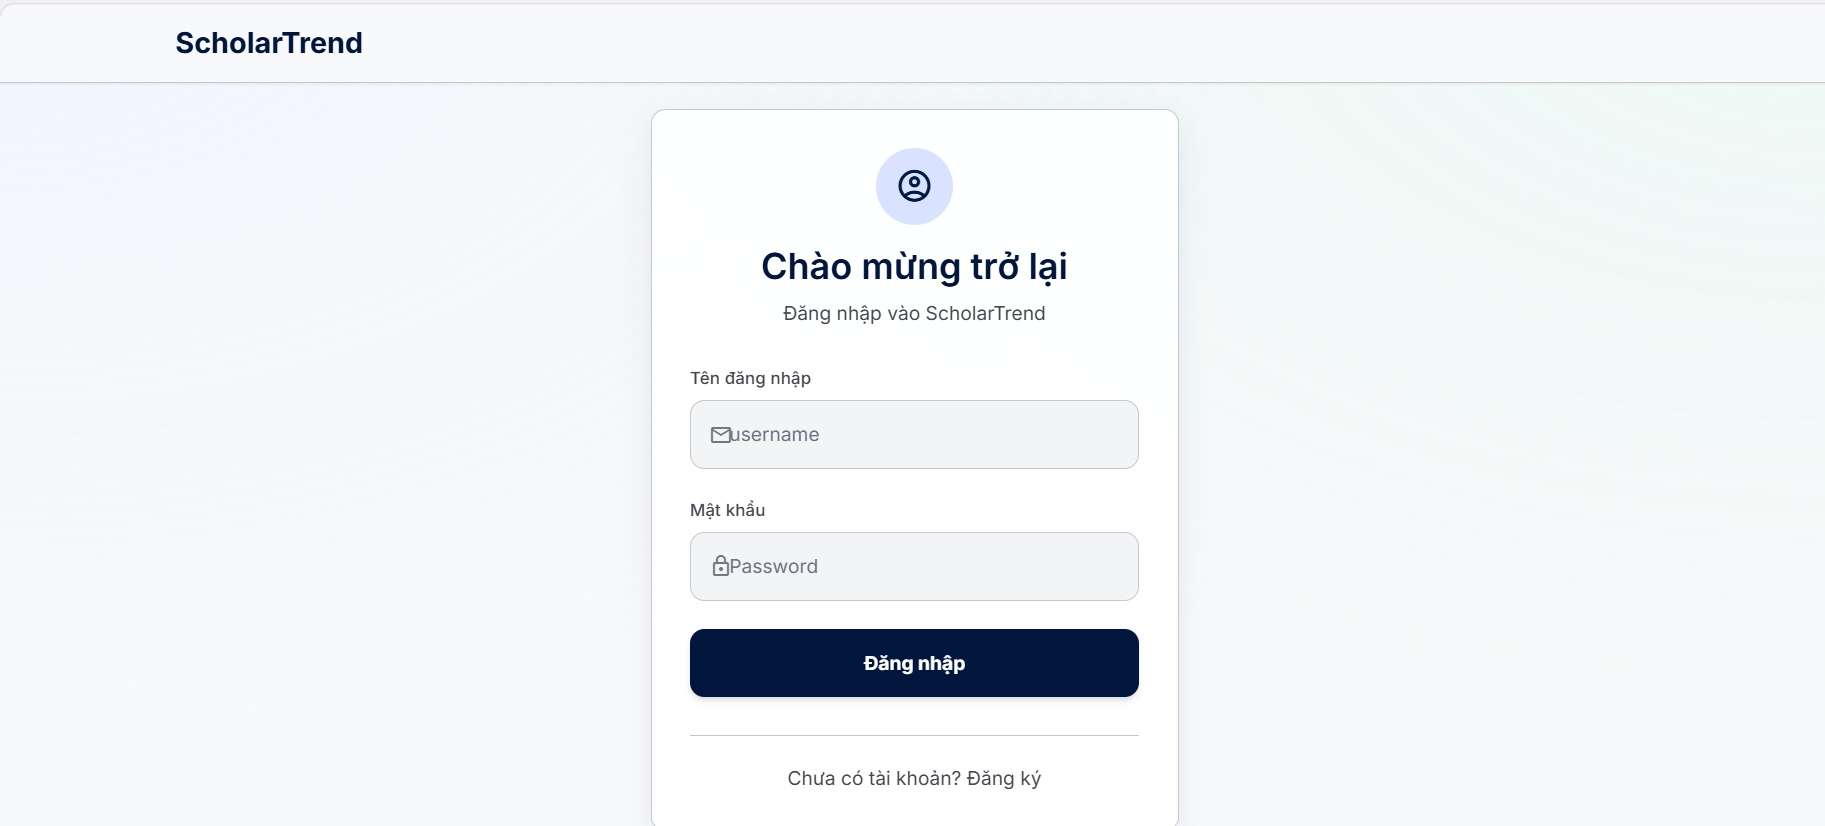
\includegraphics[width=\textwidth]{trangdangnhap.png}

	\label{fig:erd}
\end{figure}
\subsubsection{Search Papers}


\subsubsection{Search Papers}

\textbf{Role:} User

\textbf{Function trigger:} The user opens the search page, enters a keyword, selects filters (Publication Year, Open Access, Paper Type), and clicks Search.

\textbf{Function description:}

\begin{itemize}[label=-]
	\item Purpose: Allow the user to search scientific papers by keyword and filters.
	\item Data processing: Send the keyword to the search API, query OpenAlex (fallback to Crossref if it fails), apply the selected filters, and return the matching results.
\end{itemize}

\textbf{Function Details:}

\begin{itemize}[label=-]
	\item Display a search box and filters: Publication Year (from--to), Open Access toggle, Paper Type (All, Article, Review, Book-chapter, Preprint, Dataset).
	\item If Open Access is selected, only open-access papers are returned.
	\item Each result shows title (with keyword highlighted), authors, year, type, abstract, citation count, DOI link, and a Favorite button.
	\item If no results are found, display a "No matching papers found." message.
	\item If both OpenAlex and Crossref fail, display a data error message.
\end{itemize}
	

\begin{figure}[H]
	\centering
	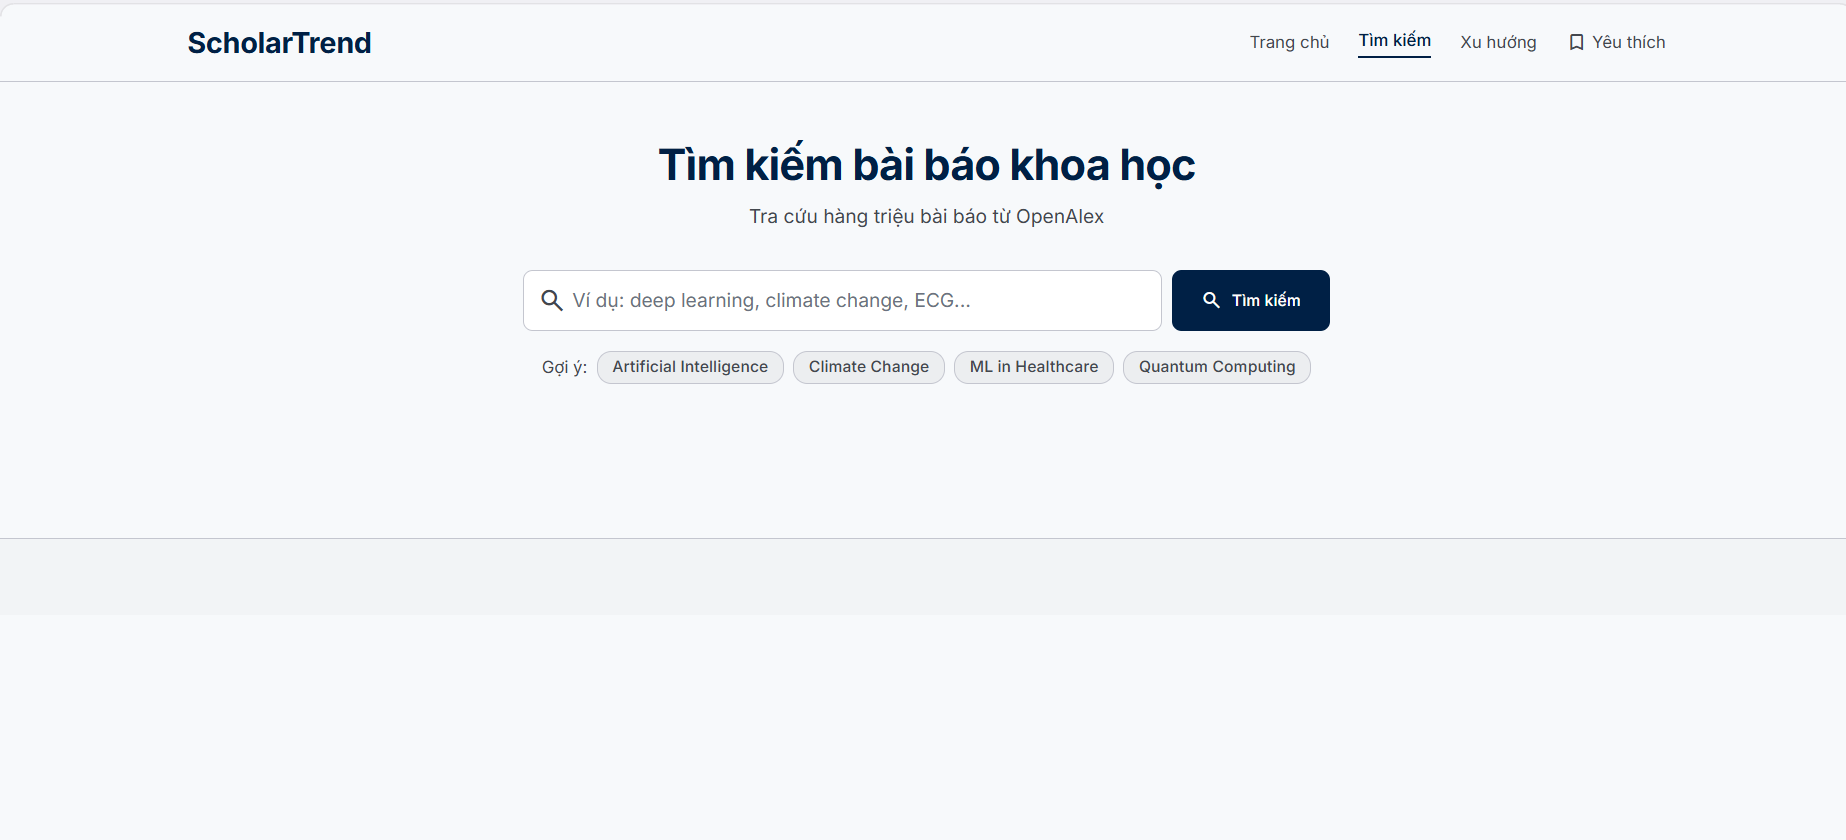
\includegraphics[width=\textwidth]{trangtimkiem.png}

	\label{fig:erd}
\end{figure}
\begin{itemize}[label=-]
	\item The start year cannot be greater than the end year.
\end{itemize}
\begin{figure}[H]
	\centering
	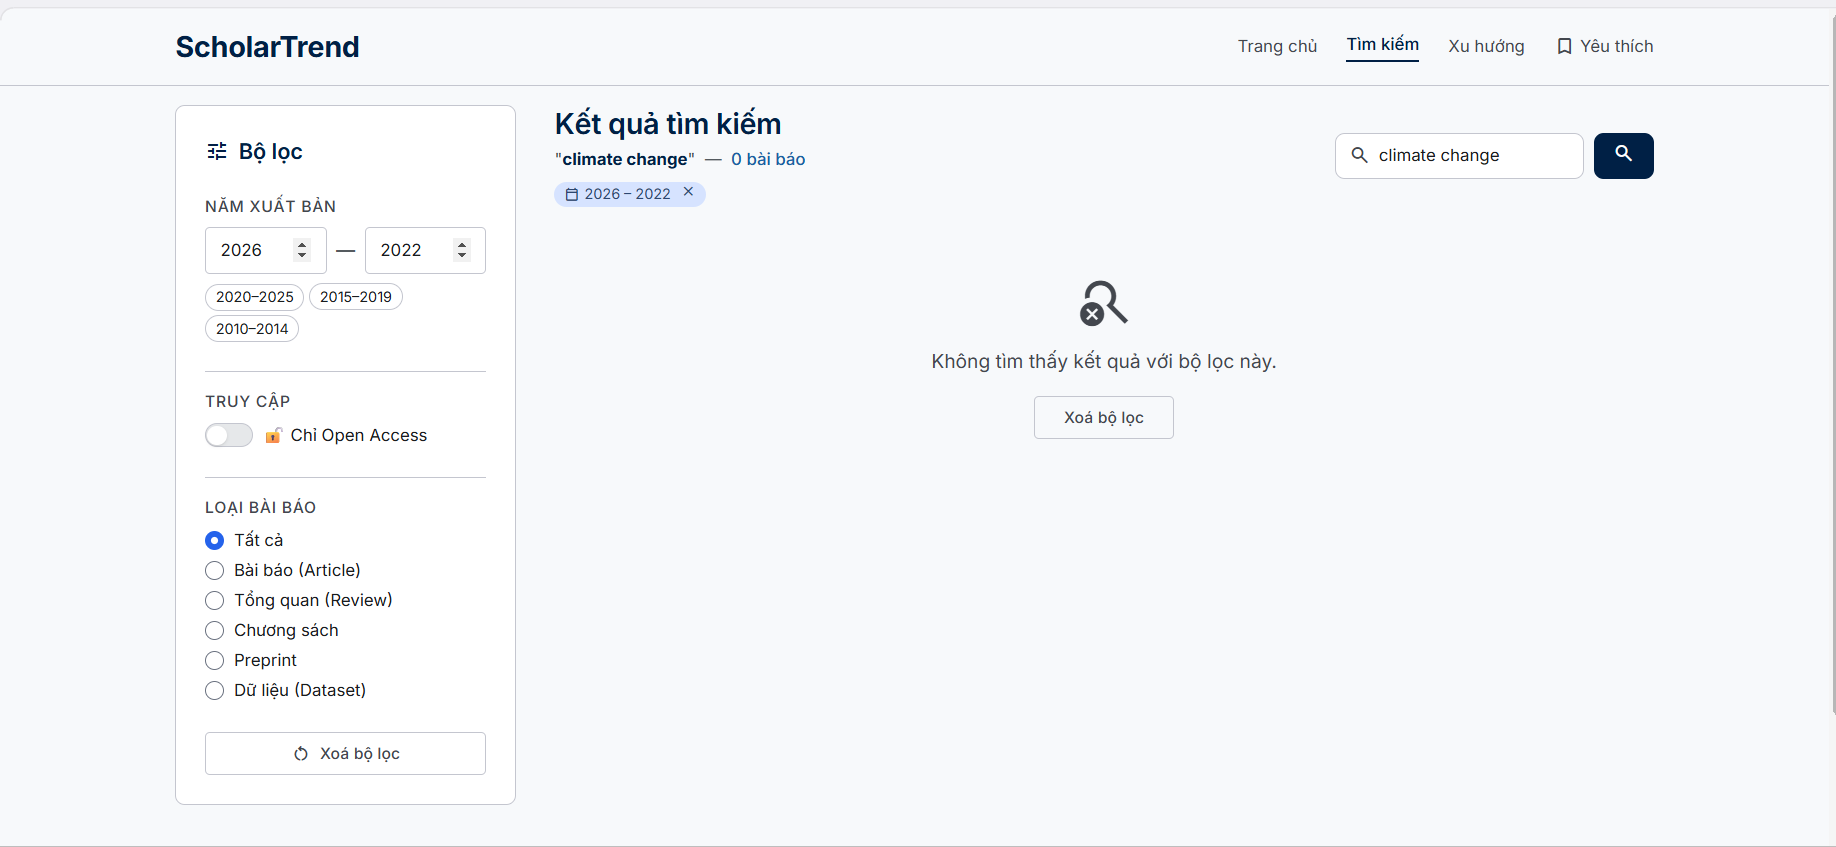
\includegraphics[width=\textwidth]{nambatdaulon.png}

	\label{fig:erd}
\end{figure}


\begin{itemize}[label=-]
	\item Search Results
\end{itemize}
\begin{figure}[H]
	\centering
	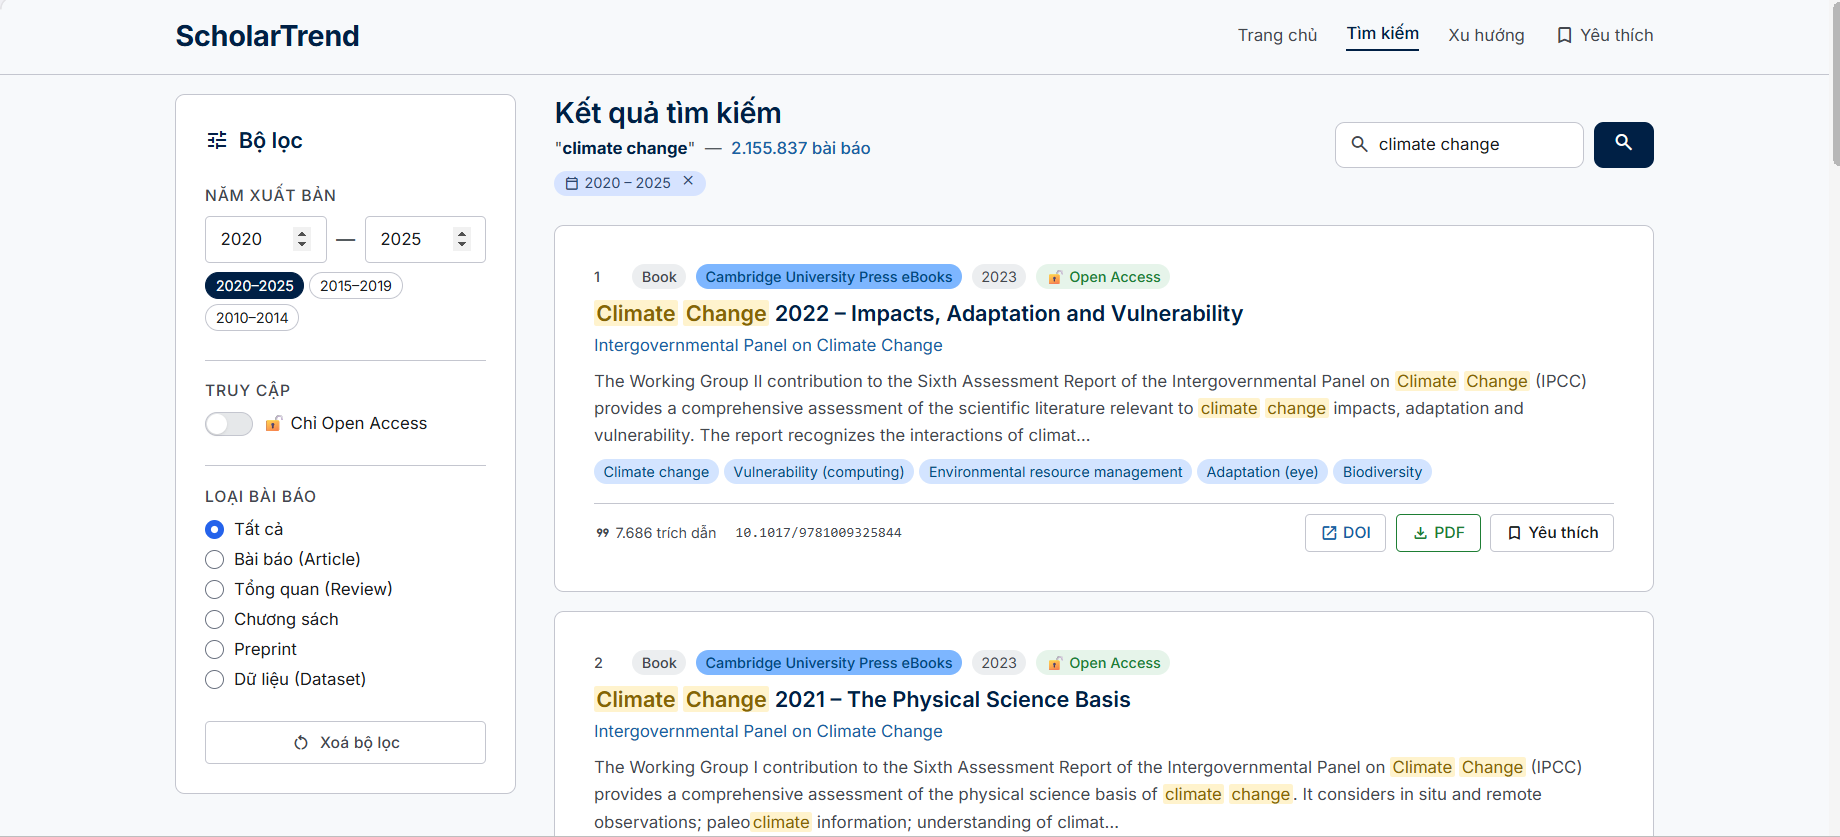
\includegraphics[width=\textwidth]{ketquatimkiem.png}

	\label{fig:erd}
\end{figure}
\subsubsection{Bookmark}


The Favorite Papers feature allows users to save publications of interest for future reference and easy access.

\begin{itemize}[label=-]
	\item Users can click the Favorite button on a paper in the Search Results page to add it to their favorite list.
	\item If the paper is successfully added, the system displays the message "Added to Favorites successfully." and updates the button status to Saved.
	\item If the selected paper already exists in the favorite list, the system displays the message "This paper is already in your Favorites." and prevents duplicate entries.
	\item Users can access the Favorites page from the navigation bar to view all saved papers.
	\item Each saved paper displays the following information:
	\begin{itemize}[label=-]
		\item Publication title.
		\item Publication year.
		\item Data source (e.g., OpenAlex).
		\item Saved date and time.
		\item DOI button for accessing the original publication.
		\item Delete button for removing the paper from the favorite list.
	\end{itemize}
	\item Users can remove a paper from the favorite list by clicking the Delete button. The system immediately updates the favorite list.
	\item Users can click the Find More Papers button to return to the search page and continue searching for publications.
\end{itemize}

\textbf{Expected Result}

\begin{itemize}[label=-]
	\item Each paper can only be saved once in the favorite list.
	\item Users can easily manage, review, and access their saved publications.
	\item All changes to the favorite list are synchronized with the database and reflected immediately in the user interface.
\end{itemize}

\begin{figure}[H]
	\centering
	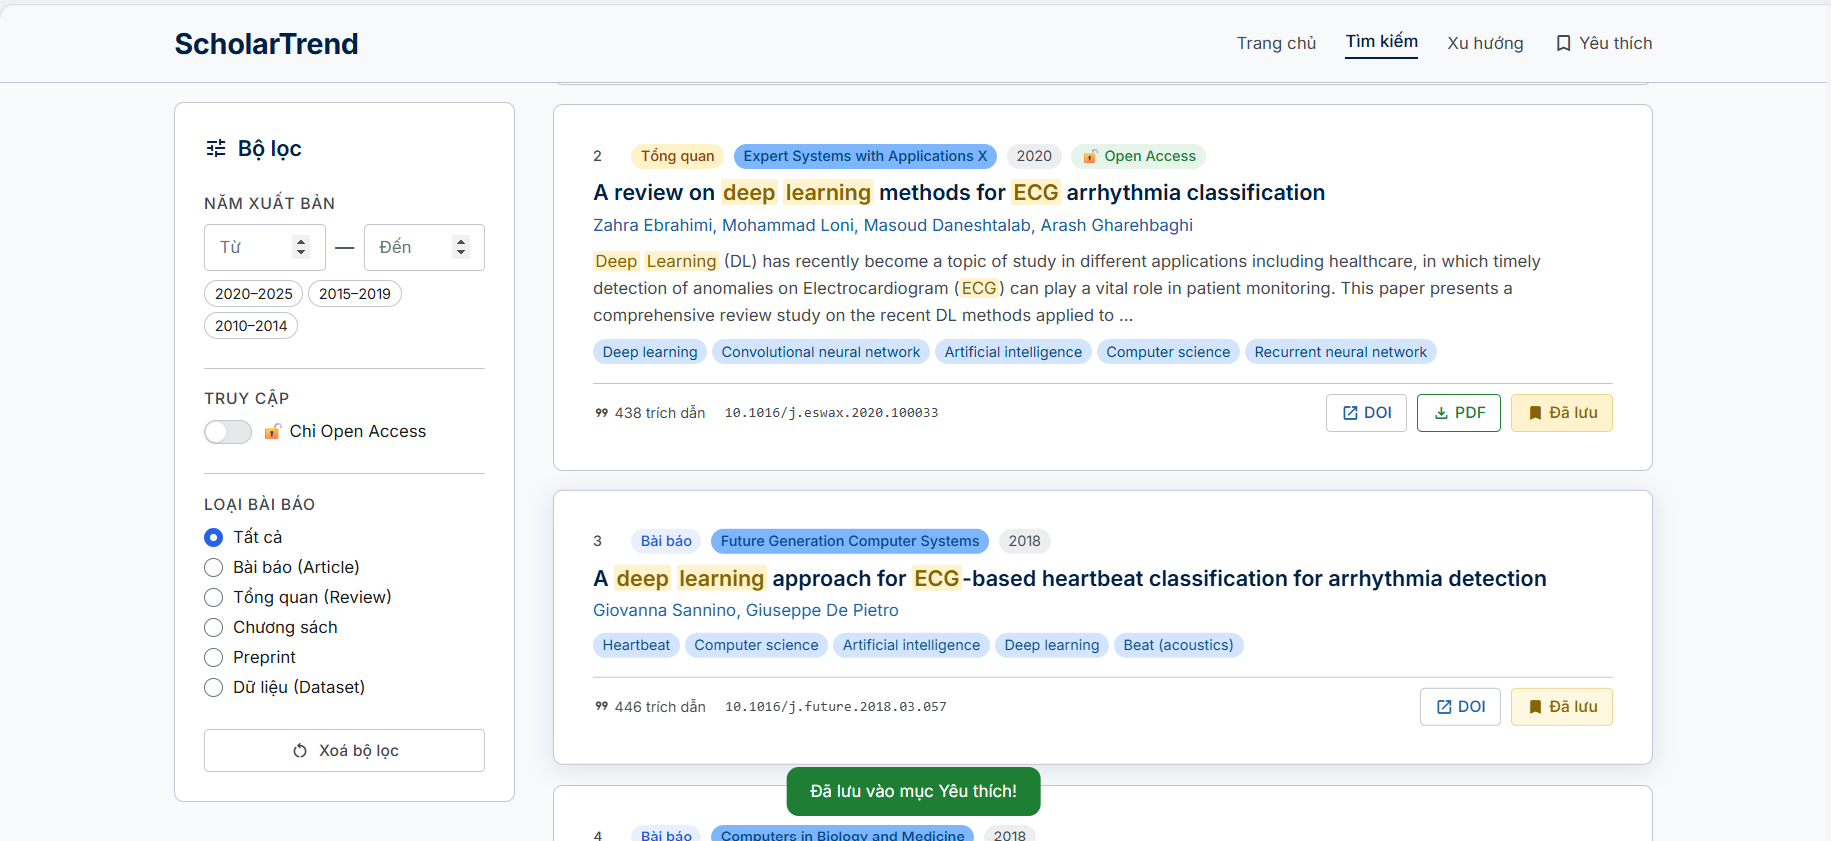
\includegraphics[width=\textwidth]{luuyeuthich.png}
	\caption{Bookmark}
	\label{fig:erd}
\end{figure}
\begin{itemize}[label=--]
	\item Marked as Favorite.
\end{itemize}
\begin{figure}[H]
	\centering
	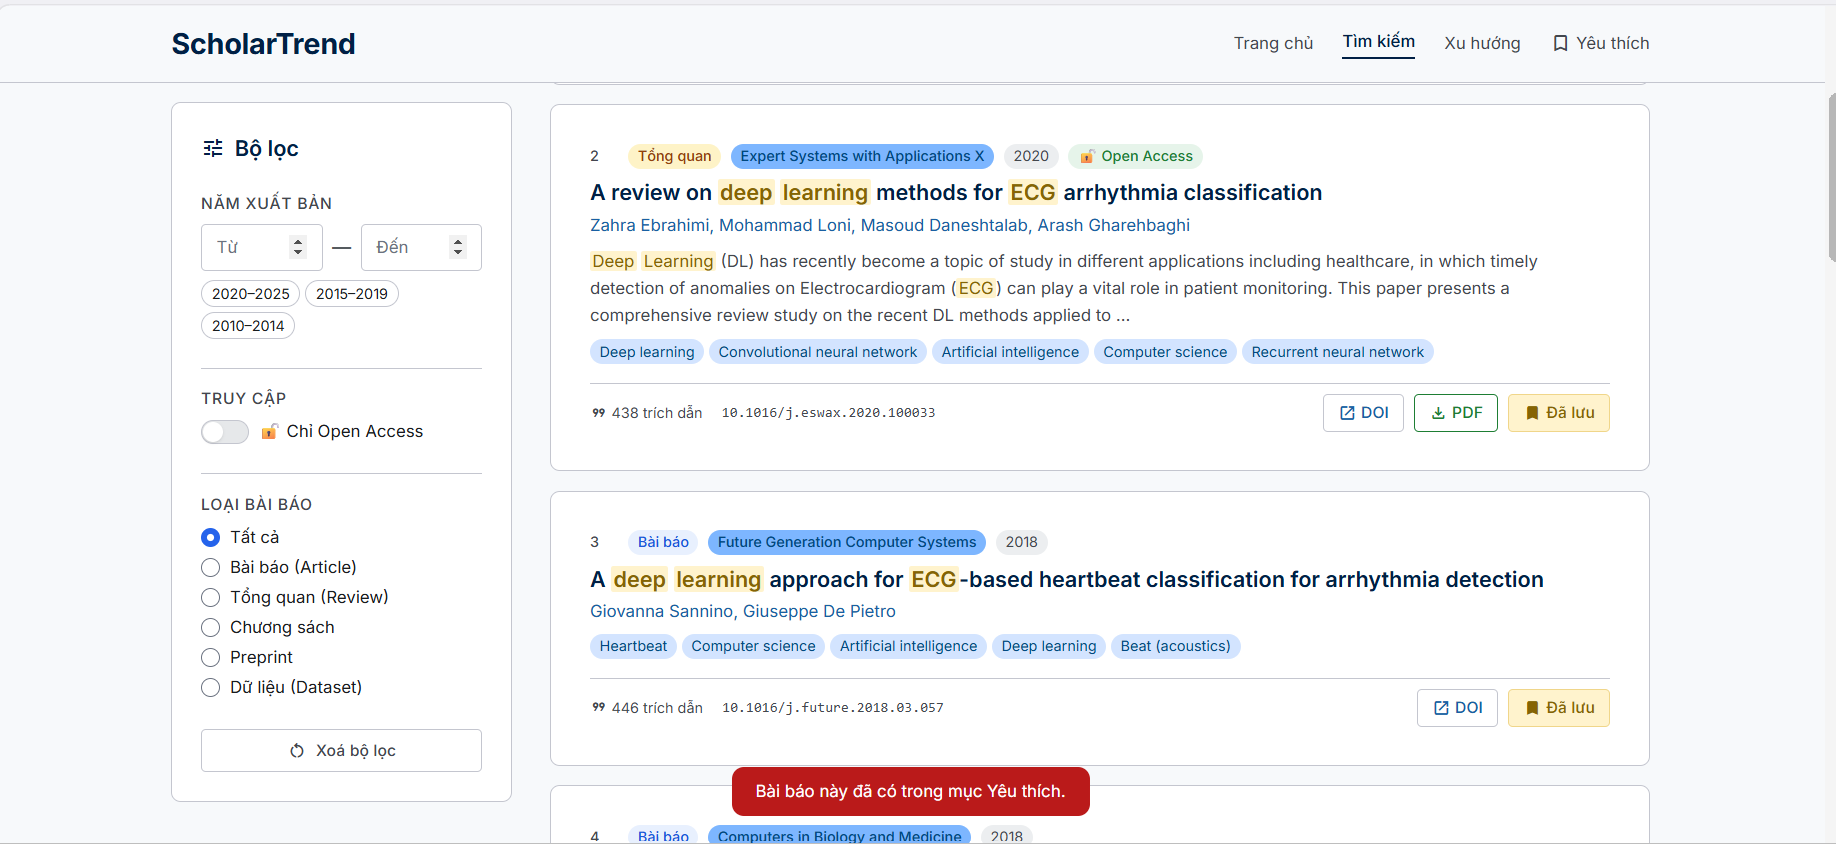
\includegraphics[width=\textwidth]{dayeuthich.png}
	\caption{Marked as Favorite.}
	\label{fig:erd}
\end{figure}
\begin{itemize}[label=--]
	\item Bookmarked List
\end{itemize}
\begin{figure}[H]
	\centering
	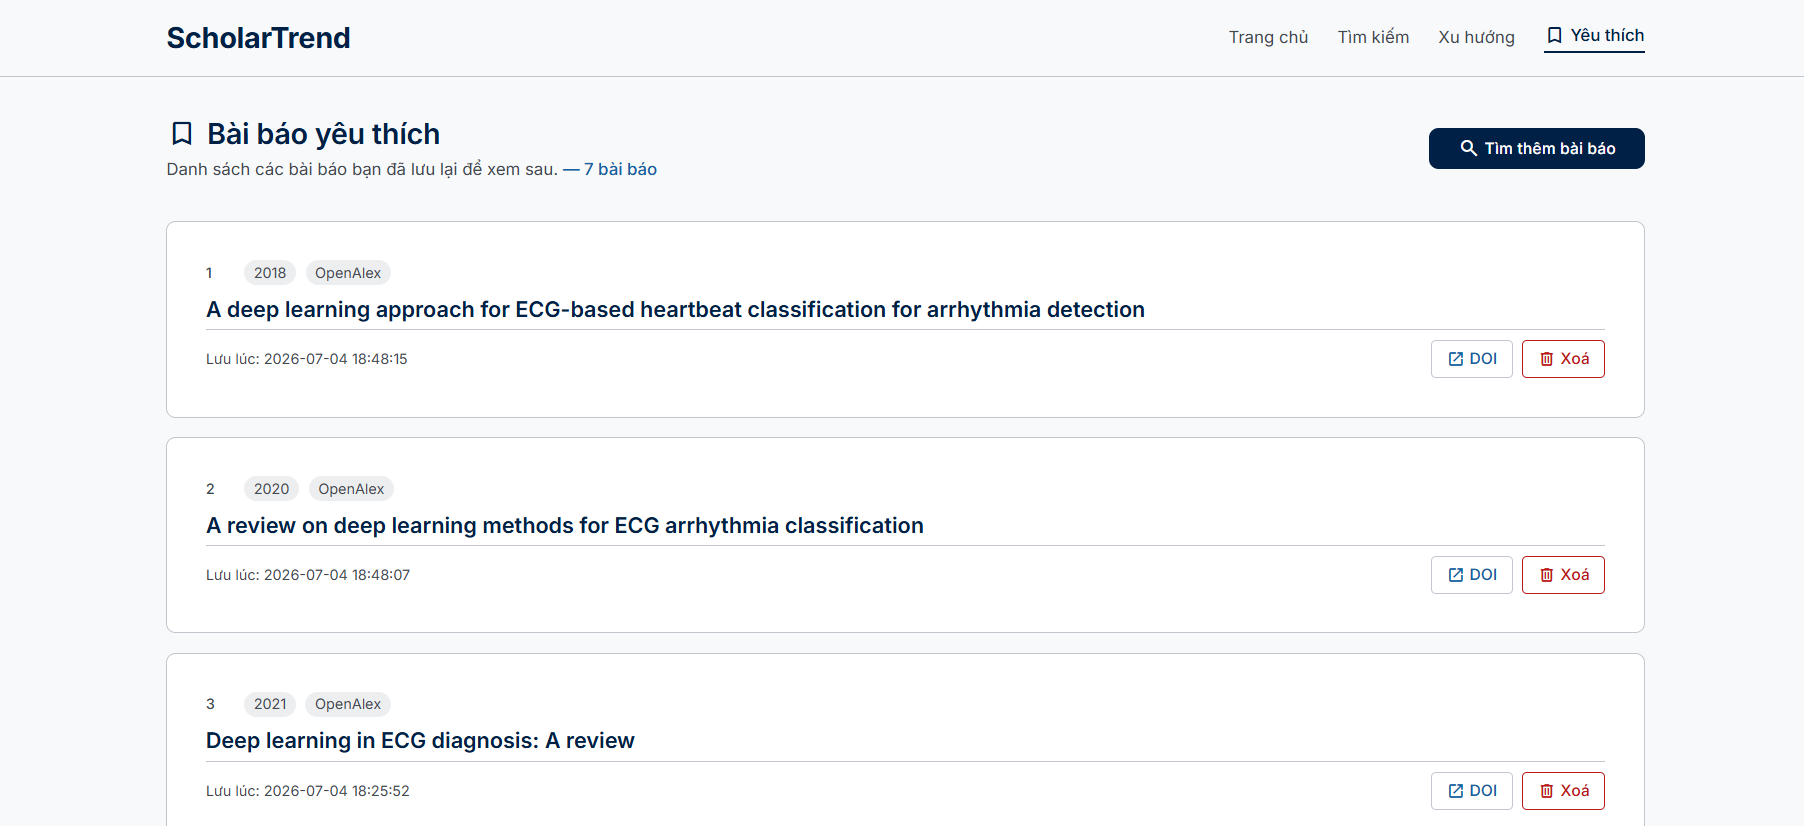
\includegraphics[width=\textwidth]{trangyeuthich.png}
	\caption{Bookmarked List}
	\label{fig:erd}
\end{figure}
\begin{itemize}[label=--]
	\item Remove from Bookmarks.
\end{itemize}
\begin{figure}[H]
	\centering
	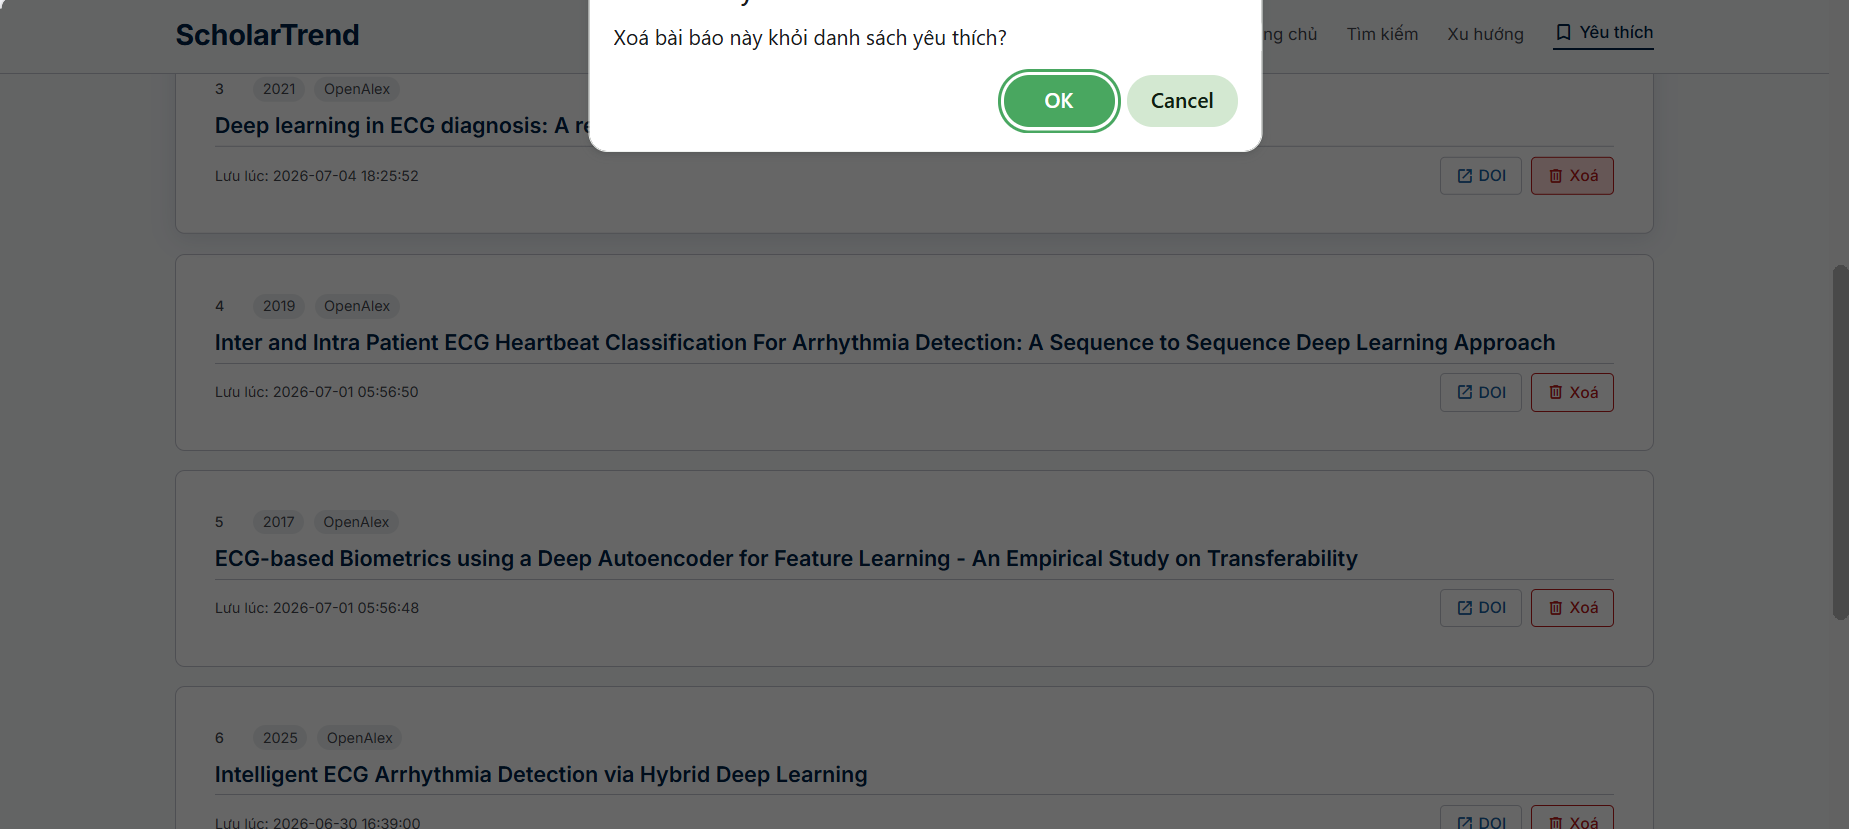
\includegraphics[width=\textwidth]{xoa.png}
	\caption{Remove from Bookmarks.}
	\label{fig:erd}
\end{figure}
\begin{itemize}[label=--]
	\item Link to the bookmarked paper.
\end{itemize}
\begin{figure}[H]
	\centering
	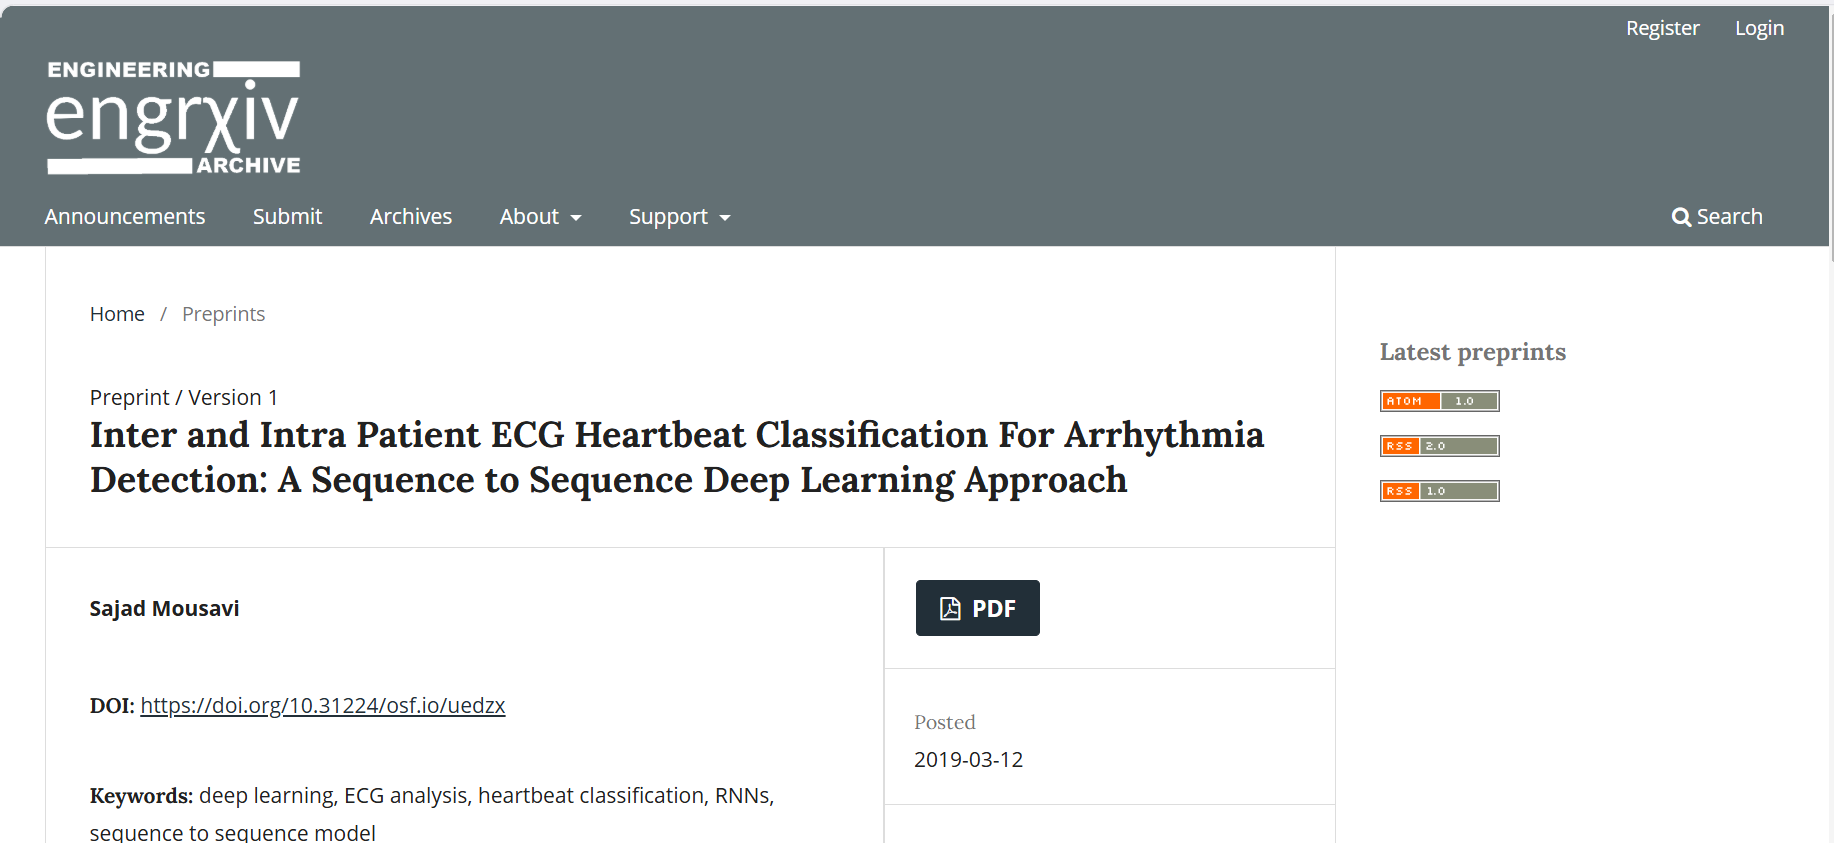
\includegraphics[width=\textwidth]{lienket.png}
	\caption{ Link to the bookmarked paper.}
	\label{fig:erd}
\end{figure}




\subsubsection{Research Trend Analysis}

\textbf{Function Trigger}
User opens \textit{Research Trend Analysis} from the main menu.
\medskip

\textbf{Function Description}
\textbf{Actors:} Researcher, Lecturer, Student
\medskip

\textbf{Purpose}
Allow users to analyze research trends of a topic within a selected time range.
\medskip

\textbf{Data Processing}
\begin{itemize}[label=-]
	\item Validate the topic and time range.
	\item Retrieve publication data from the Crossref API.
	\item Calculate statistics and generate charts.
	\item Display the trend dashboard.
\end{itemize}
\medskip

\textbf{Interface}
\begin{itemize}[label=-]
	\item Topic search bar, time range selector, \textbf{Analyze} button.
	\item Two tabs: Dashboard, Trending Topics.
	\item Widgets: Total Publications, Total Citations, Open Access Ratio, Trend Growth.
	\item Charts: Publications by Year, Top Keywords, Top Journals, Top Authors, Featured Publications.
\end{itemize}
\medskip

\textbf{Validation}
\begin{itemize}[label=-]
	\item Keyword cannot be empty.
	\item Start Year must not be greater than End Year.
\end{itemize}
\medskip

\textbf{Business Rules}
\begin{itemize}[label=-]
	\item Statistics are calculated from data retrieved via the Crossref API.
	\item Trend Growth is compared with the previous period of the same duration.
	\item Users can follow/unfollow a trending topic.
	\item The dashboard refreshes when the topic or time range changes.
\end{itemize}
\medskip

\textbf{Normal Flow}
\begin{enumerate}
	\item Enter a topic, select a time range, click Analyze.
	\item The system validates input and retrieves data from the API.
	\item Statistics are calculated and results shown on the dashboard.
\end{enumerate}
\medskip

\textbf{Exceptions}
\begin{itemize}[label=-]
	\item No data found $\rightarrow$ \textit{"No data available."}
	\item Invalid time range $\rightarrow$ request the user to correct it.
	\item API error $\rightarrow$ \textit{"Unable to load data. Please try again later."}
\end{itemize}
\begin{figure}[H]
	\centering
	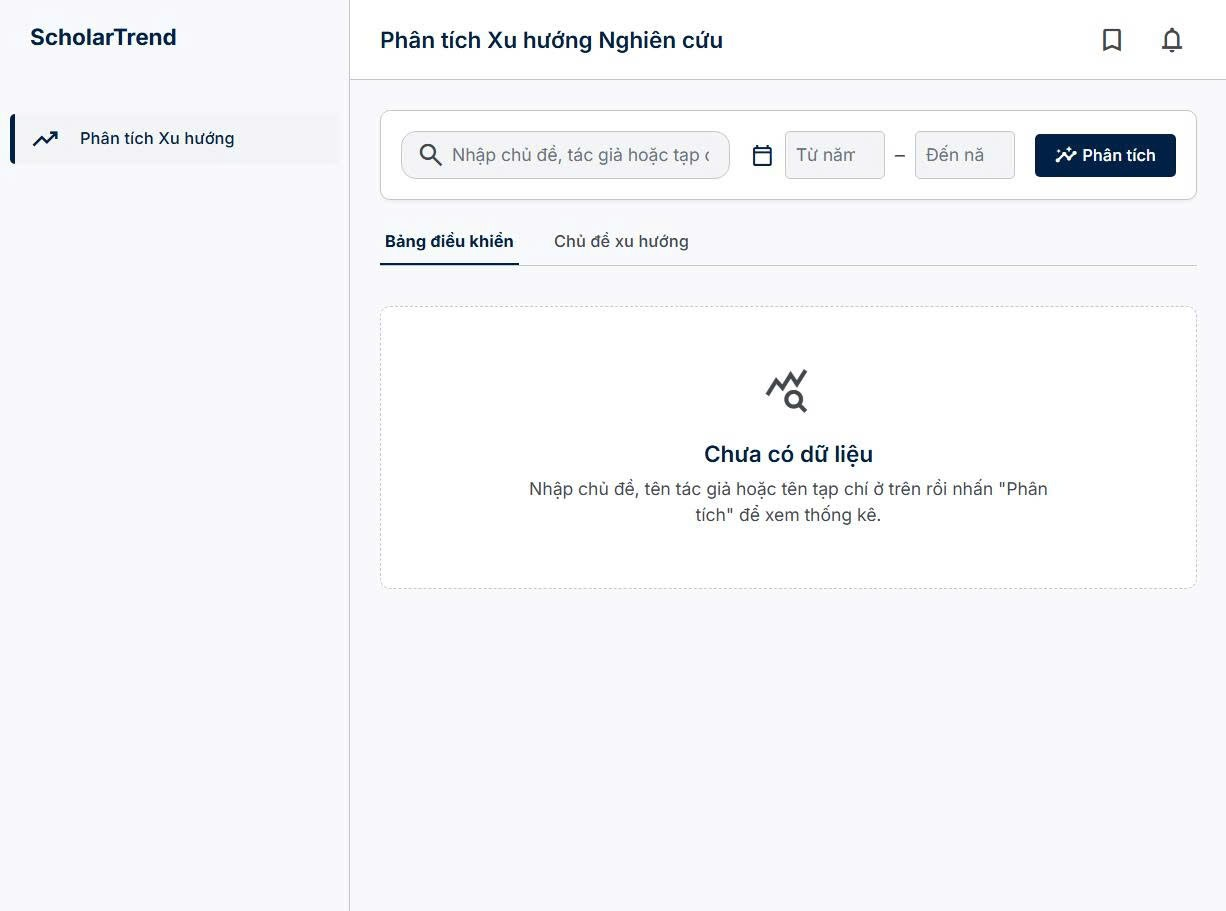
\includegraphics[width=\textwidth]{ptxh.png}

	\label{fig:erd}
	
\end{figure}
\begin{itemize}[label=-]
	\item Please enter a search keyword.
\end{itemize}
\begin{figure}[H]
	\centering
	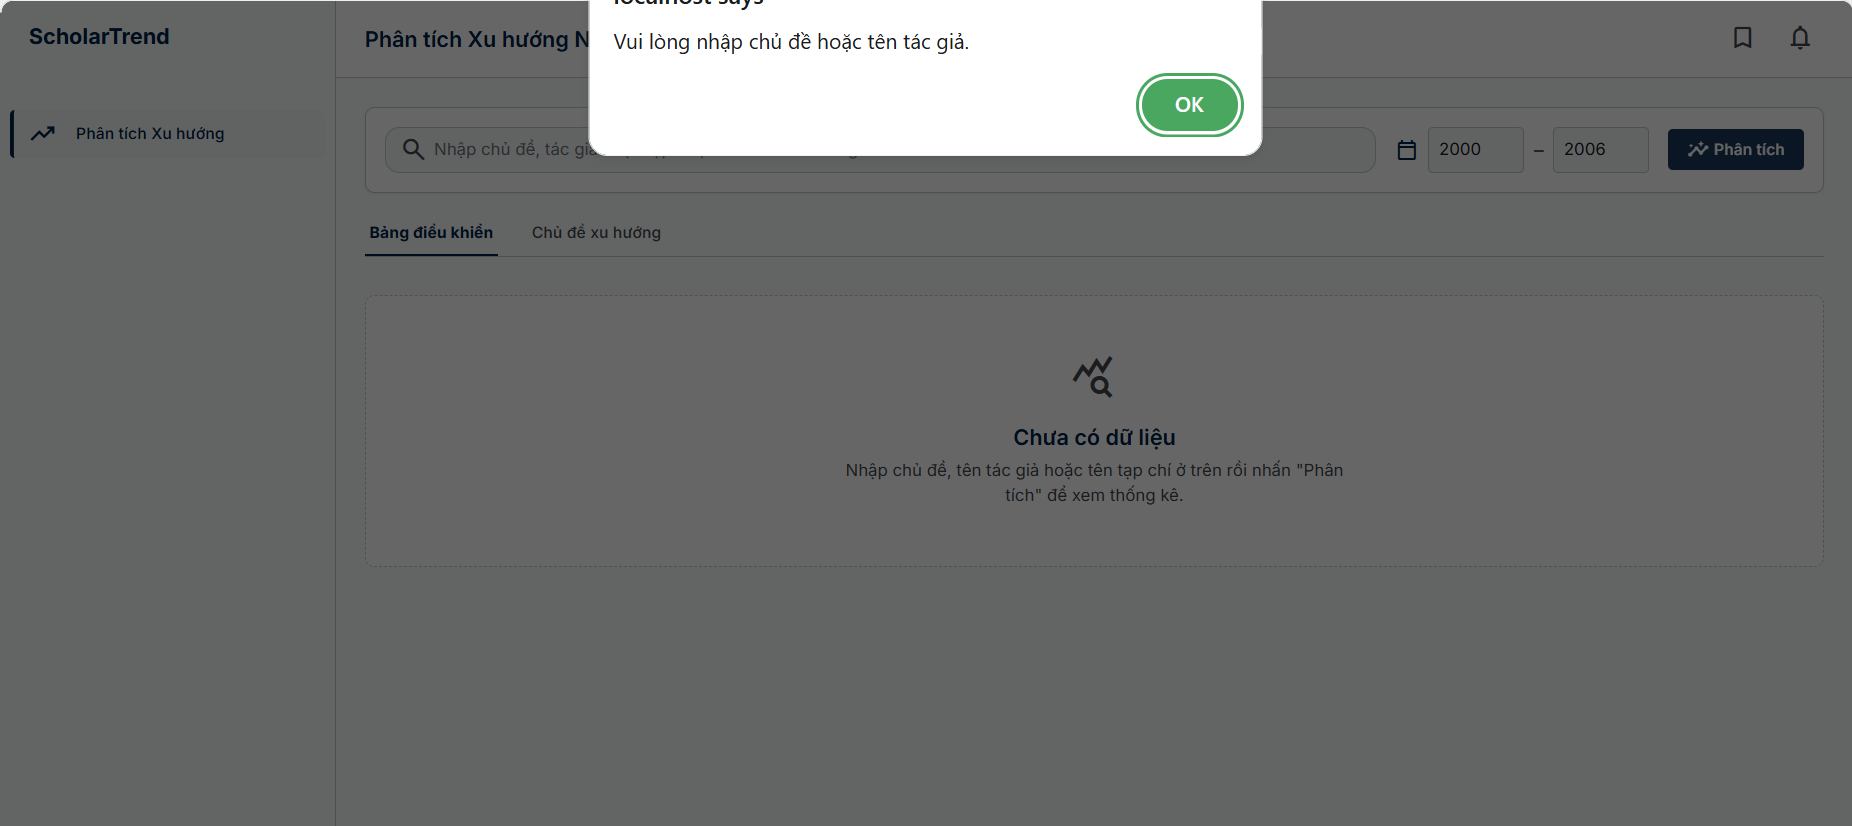
\includegraphics[width=\textwidth]{thieu.png}

	\label{fig:erd}
\end{figure}
\begin{itemize}[label=-]
	\item The start year cannot be greater than the end year.
\end{itemize}

\begin{figure}[H]
	\centering
	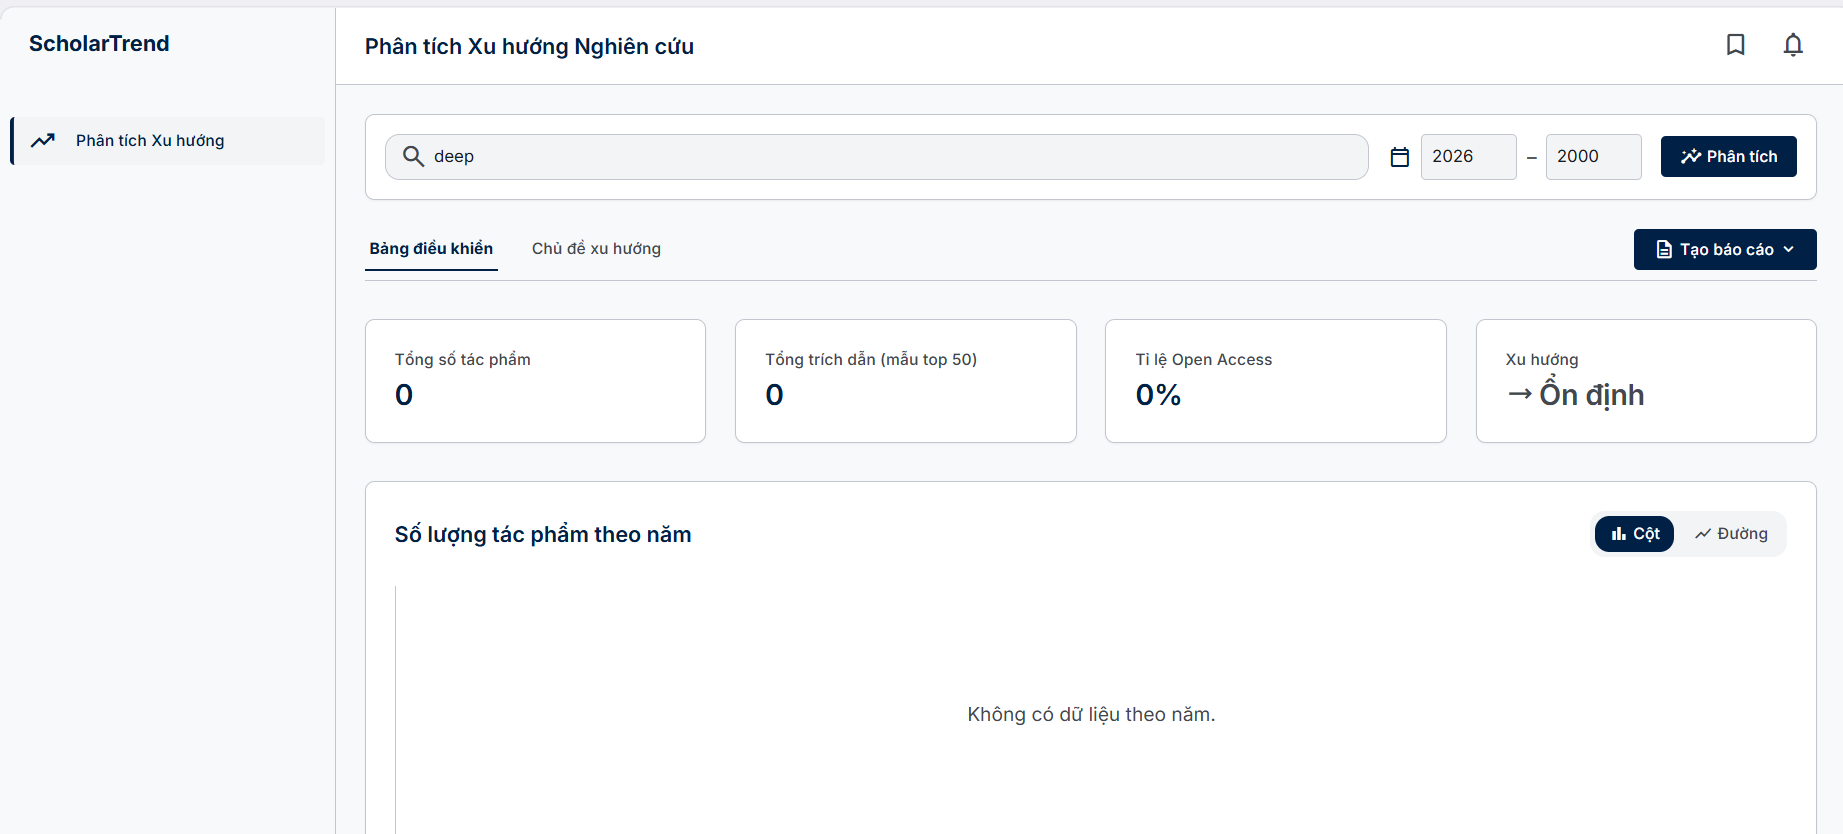
\includegraphics[width=\textwidth]{batdaulonhon.png}

	\label{fig:erd}
\end{figure}
\begin{itemize}[label=-]
	\item Analysis Results.
\end{itemize}
\begin{figure}[H]
	\centering
	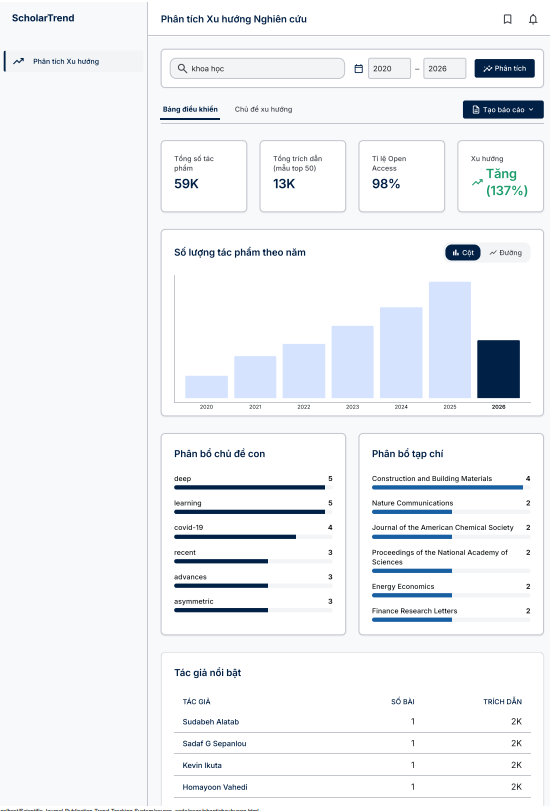
\includegraphics[width=\textwidth]{ketquaphantich1.png}

	\label{fig:erd}
\end{figure}
\begin{figure}[H]
	\centering
	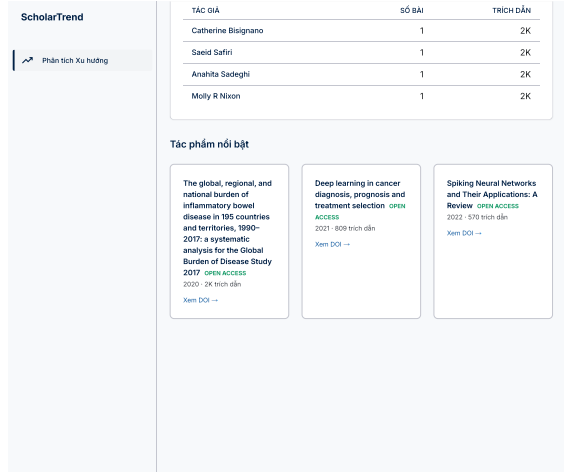
\includegraphics[width=\textwidth]{ketquaphantich2.png}

	\label{fig:erd}
\end{figure}









\subsubsection{Export Research Trend Report}

\textbf{Function Trigger}
User opens \textit{Research Trend Analysis} $\rightarrow$ enters a topic and time range $\rightarrow$ clicks Analyze $\rightarrow$ clicks Generate Report $\rightarrow$ selects an export option (Preview \& Print / Save PDF, Download PDF, Download HTML).
\medskip

\textbf{Function Description}
\textbf{Actors:} Researcher, Lecturer, Student
\medskip

\textbf{Purpose}
Allow users to export the trend analysis results into different report formats for printing, sharing, or offline viewing.
\medskip

\textbf{Data Processing}
\begin{itemize}[label=-]
	\item Verify the analysis is completed and data is available.
	\item Collect current results: statistics, charts, Trending Topics, Top Journals/Authors/Keywords, Featured Publications.
	\item Generate the report in the selected format and prepare it for preview or download.
\end{itemize}
\medskip

\textbf{Validation}
\begin{itemize}[label=-]
	\item Analysis must be completed and report data must be available before exporting.
\end{itemize}
\medskip

\textbf{Business Rules}
\begin{itemize}[label=-]
	\item The report contains the currently displayed analysis results.
	\item Export options: Preview \& Print / Save PDF, Download PDF, Download HTML.
	\item The report reflects the selected topic/time range and preserves dashboard layout and chart formatting.
\end{itemize}
\medskip

\textbf{Normal Flow}
\begin{enumerate}
	\item Complete the analysis, click Generate Report, select an export format.
	\item The system validates data, generates the report.
	\item The report is previewed or downloaded.
\end{enumerate}
\medskip

\textbf{Exceptions}

\begin{figure}[H]
	\centering
	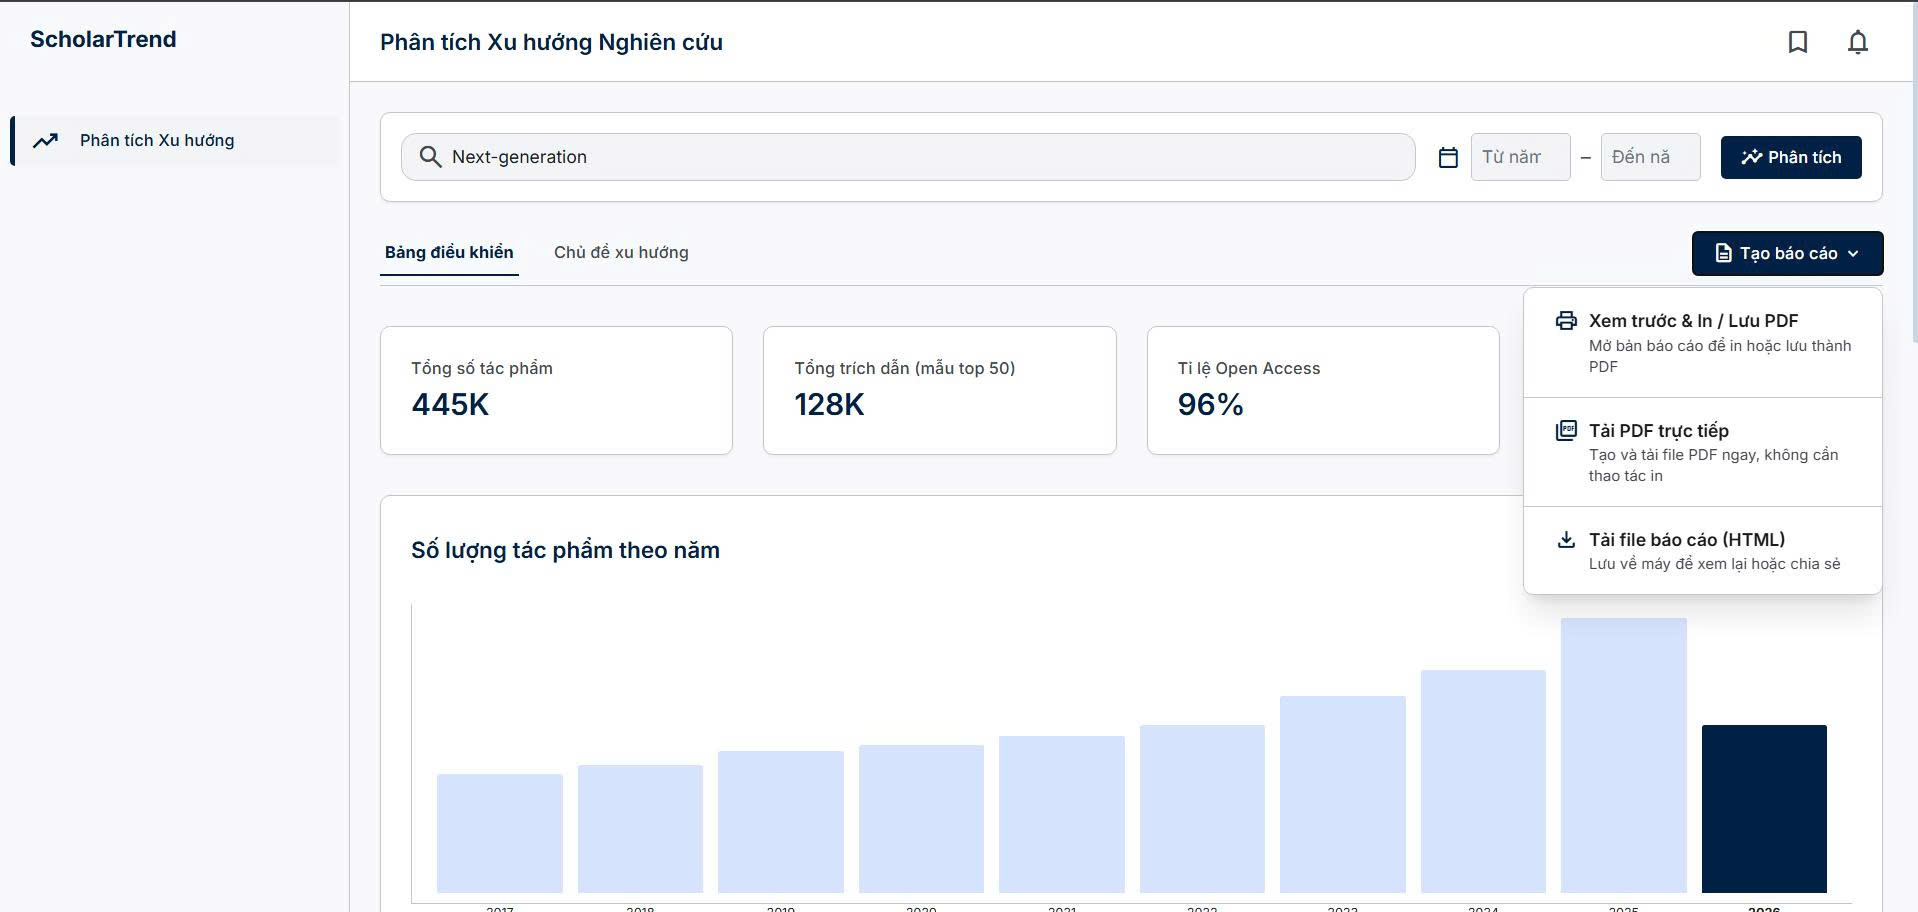
\includegraphics[width=\textwidth]{tbc.jpg}
	\caption{Generate Report}
	\label{fig:erd}
\end{figure}
\begin{itemize}[label=-]
	\item Export Report.
\end{itemize}
\begin{figure}[H]
	\centering
	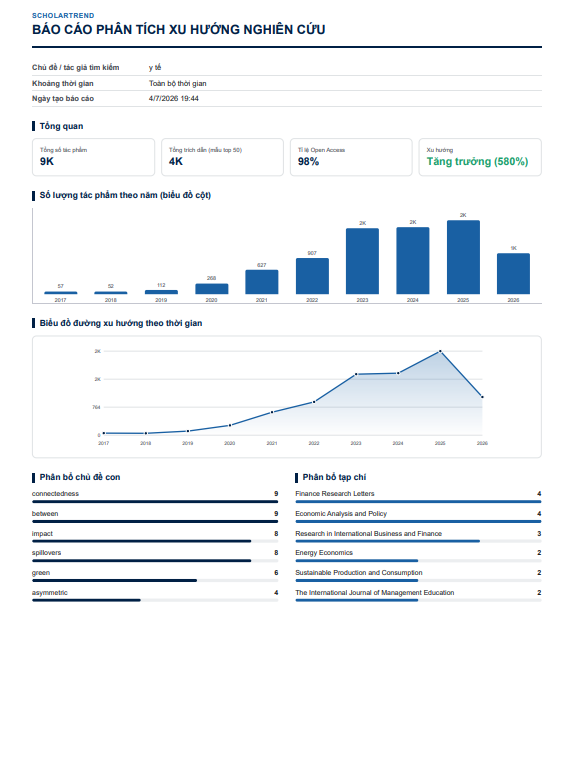
\includegraphics[width=\textwidth]{xuatbaocao.png}
	\caption{Export Report.}
	\label{fig:erd}
\end{figure}
\subsubsection{Follow Topic}


\textbf{Function Activation}
User opens \textit{Trend Analysis} $\rightarrow$ enters a topic and time range $\rightarrow$ clicks Analyze $\rightarrow$ clicks Follow.
\medskip

\textbf{Description}
\textbf{Actors:} Researcher, Lecturer, Student
\medskip

\textbf{Purpose}
Allow users to follow topics of interest for easier management and quick access.
\medskip

\textbf{Data Processing}
\begin{itemize}[label=-]
	\item Verify the user is logged in.
	\item Check if the topic is already followed; if not, save it and update status to Following.
	\item Prevent duplicate entries if already followed.
	\item Allow viewing and unfollowing topics from the followed list.
	\item Update the list after each follow/unfollow action.
\end{itemize}
\medskip

\textbf{Result}
\begin{itemize}[label=-]
	\item The topic is added to the followed list.
	\item The list is updated correctly.
	\item Users can follow/unfollow topics at any time.
\end{itemize}
\begin{figure}[H]
	\centering
	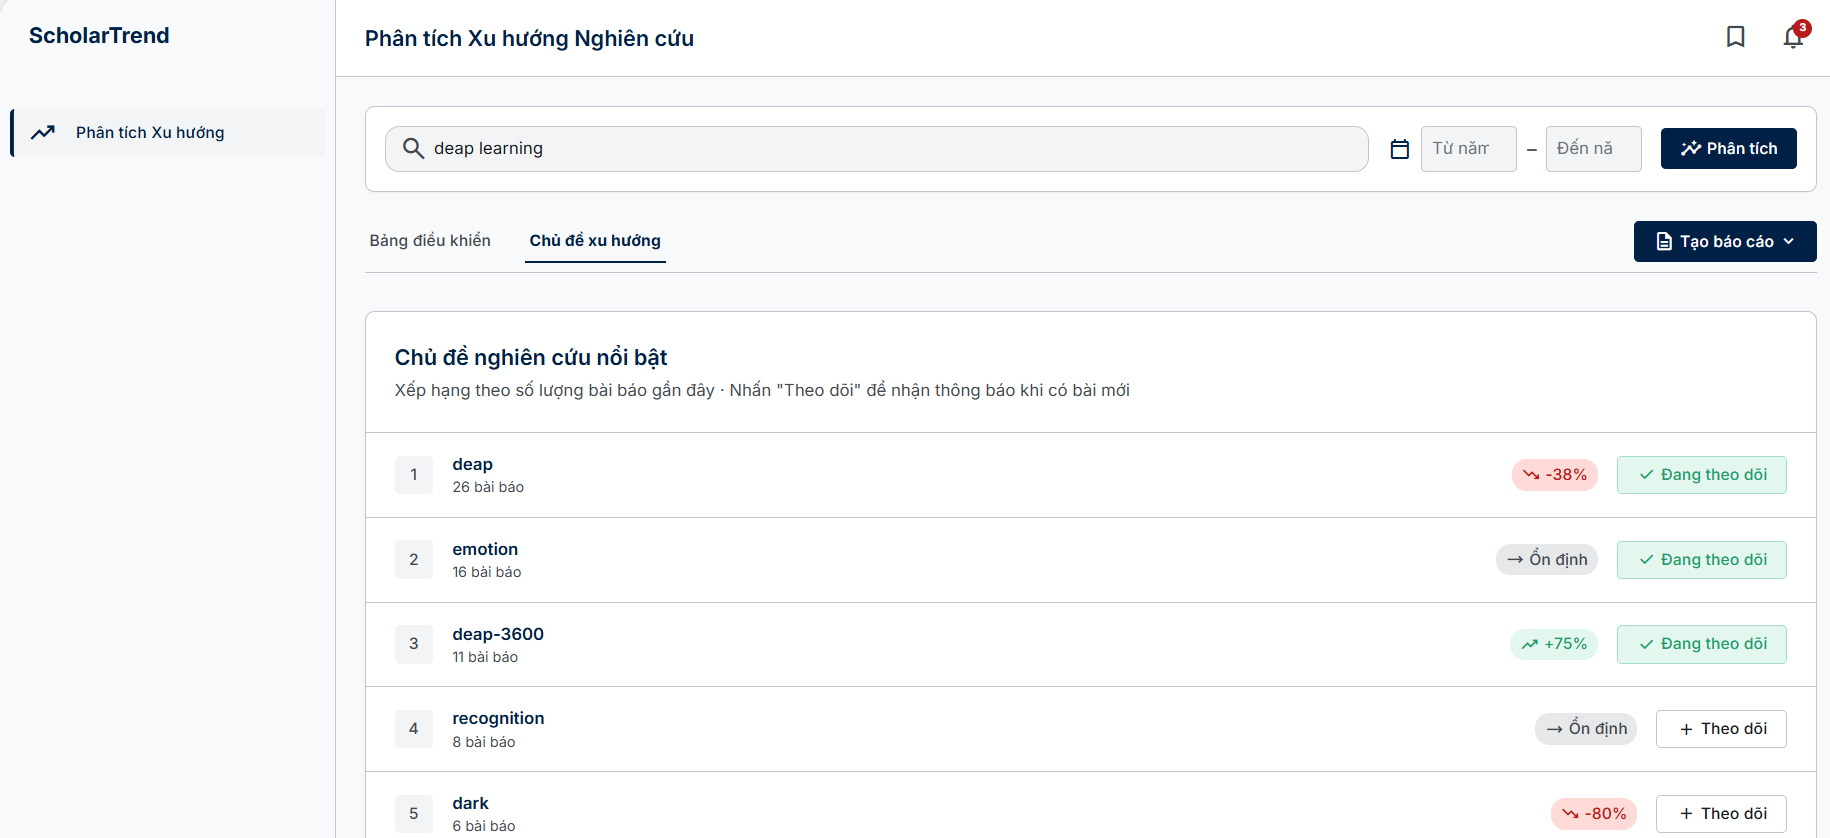
\includegraphics[width=\textwidth]{theodoi.png}

	\label{fig:erd}
\end{figure}
\begin{itemize}[label=-]
	\item Follow topics list
\end{itemize}
\begin{figure}[H]
	\centering
	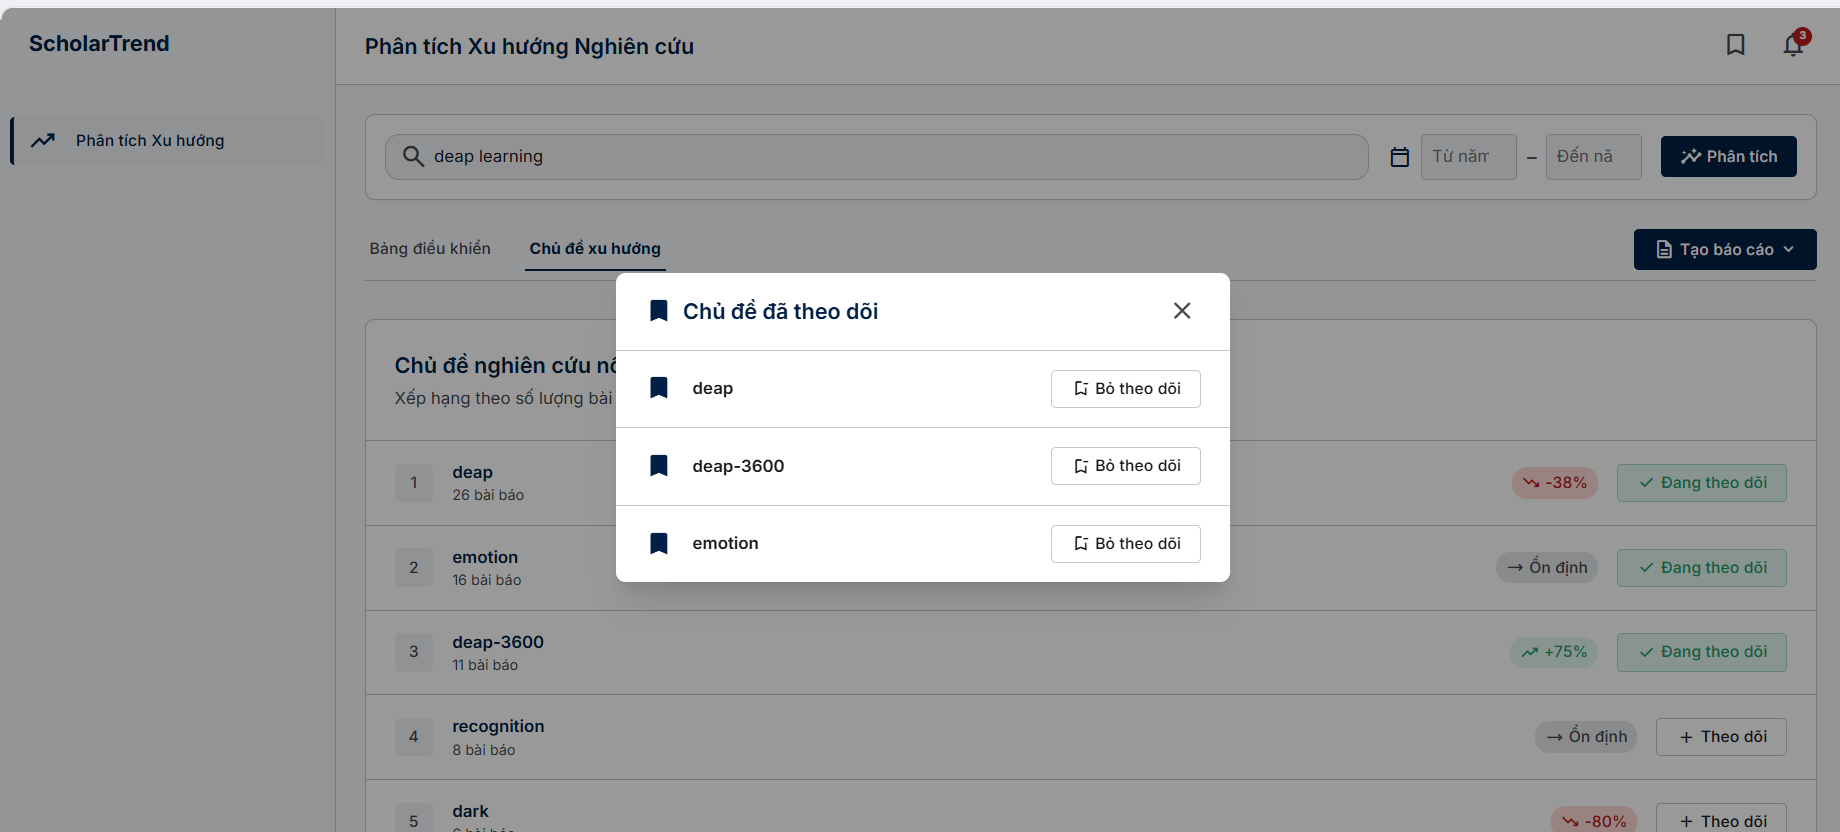
\includegraphics[width=\textwidth]{dstheodoi.png}

	\label{fig:erd}
\end{figure}
\begin{itemize}[label=-]
	\item Unfollow topic
\end{itemize}
\begin{figure}[H]
	\centering
	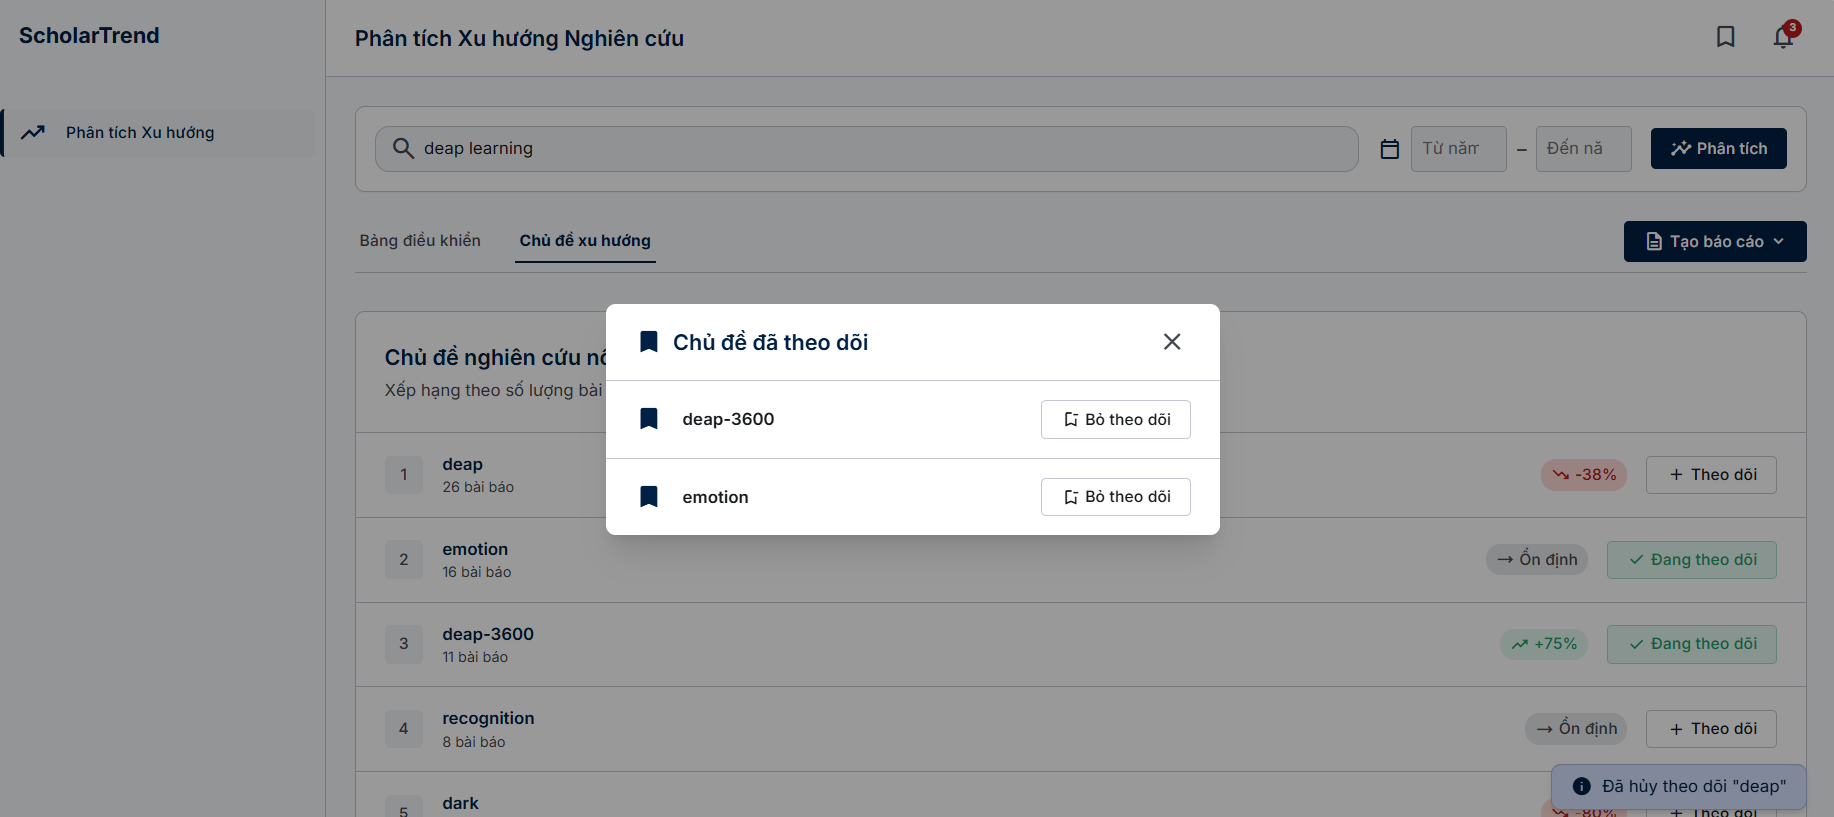
\includegraphics[width=\textwidth]{huytheodoi.png}

	\label{fig:erd}
\end{figure}
\subsubsection{Receive Notifications}
\textbf{Function Activation}
User logs into the system. Notifications automatically appear when new ones are available.
\medskip

\textbf{Description}
\textbf{Actors:} Researcher, Lecturer, Student
\medskip

\textbf{Purpose}
Allow users to receive notifications about followed topics and system announcements from administrators.
\medskip

\textbf{Data Processing}
\begin{itemize}[label=-]
	\item Verify the user is logged in.
	\item Retrieve unread notifications from the database.
	\item Display notifications for followed topics and admin announcements.
	\item Allow users to mark notifications as read and update their status.
\end{itemize}
\medskip

\textbf{Result}
\begin{itemize}[label=-]
	\item Users receive notifications about followed topics and admin announcements.
	\item Notification status updates correctly after being read.
\end{itemize}
\begin{figure}[H]
	\centering
	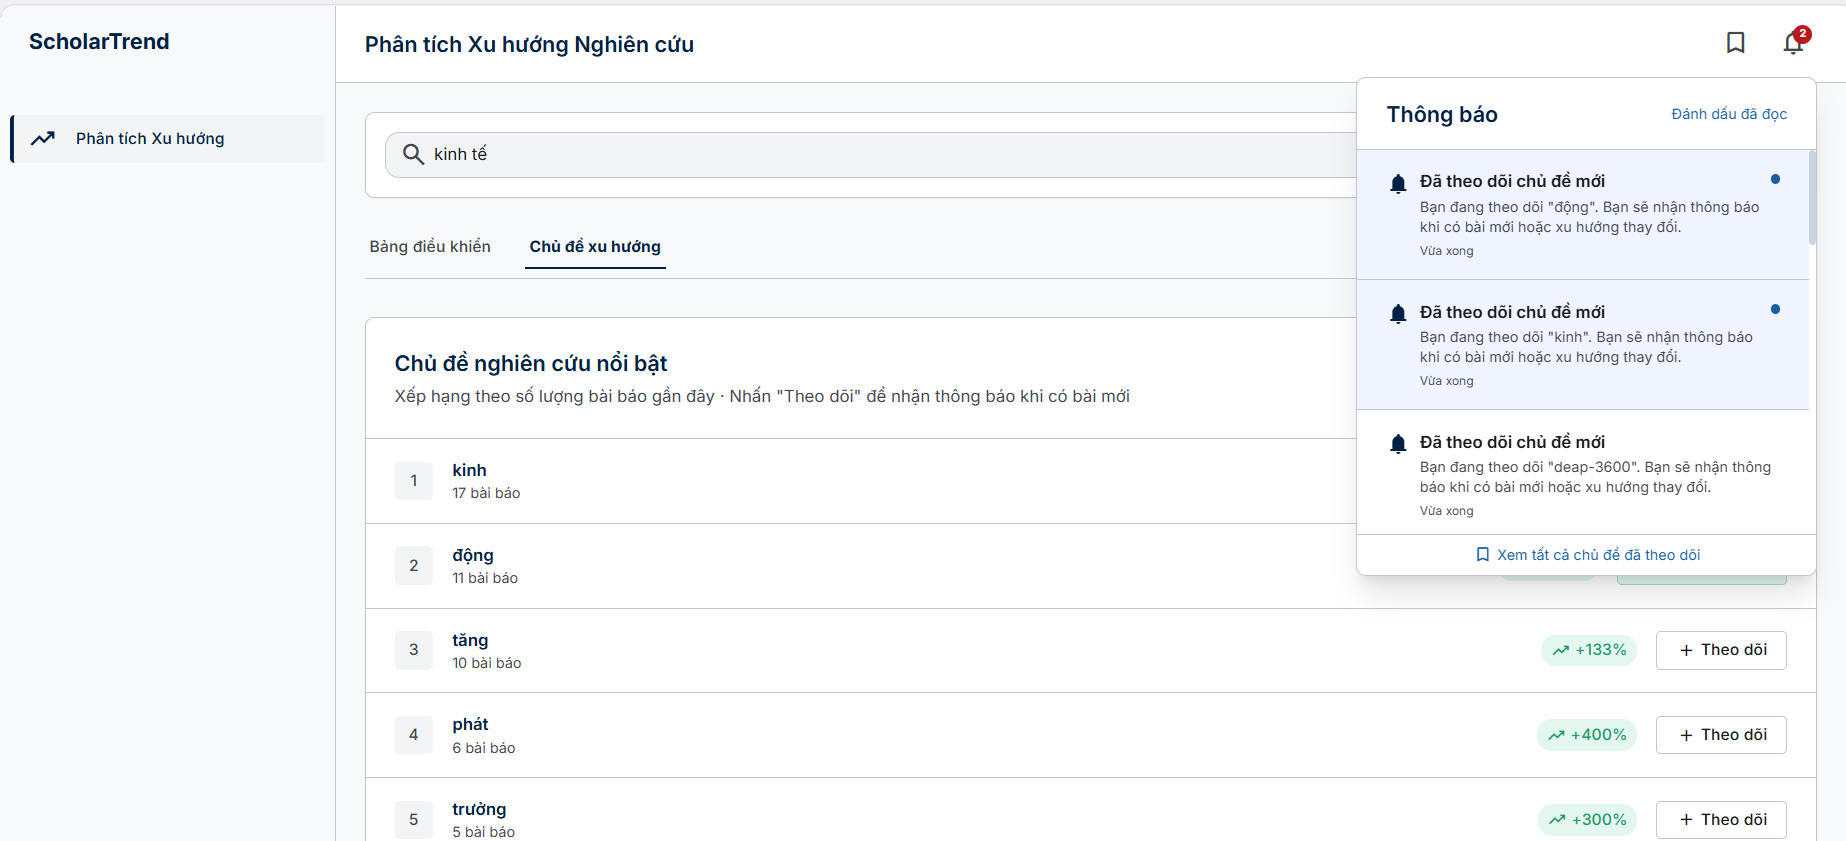
\includegraphics[width=\textwidth]{nhanthongbao.png}

	\label{fig:erd}
\end{figure}
\begin{itemize}[label=-]
	\item Mark as Read.
\end{itemize}
\begin{figure}[H]
	\centering
	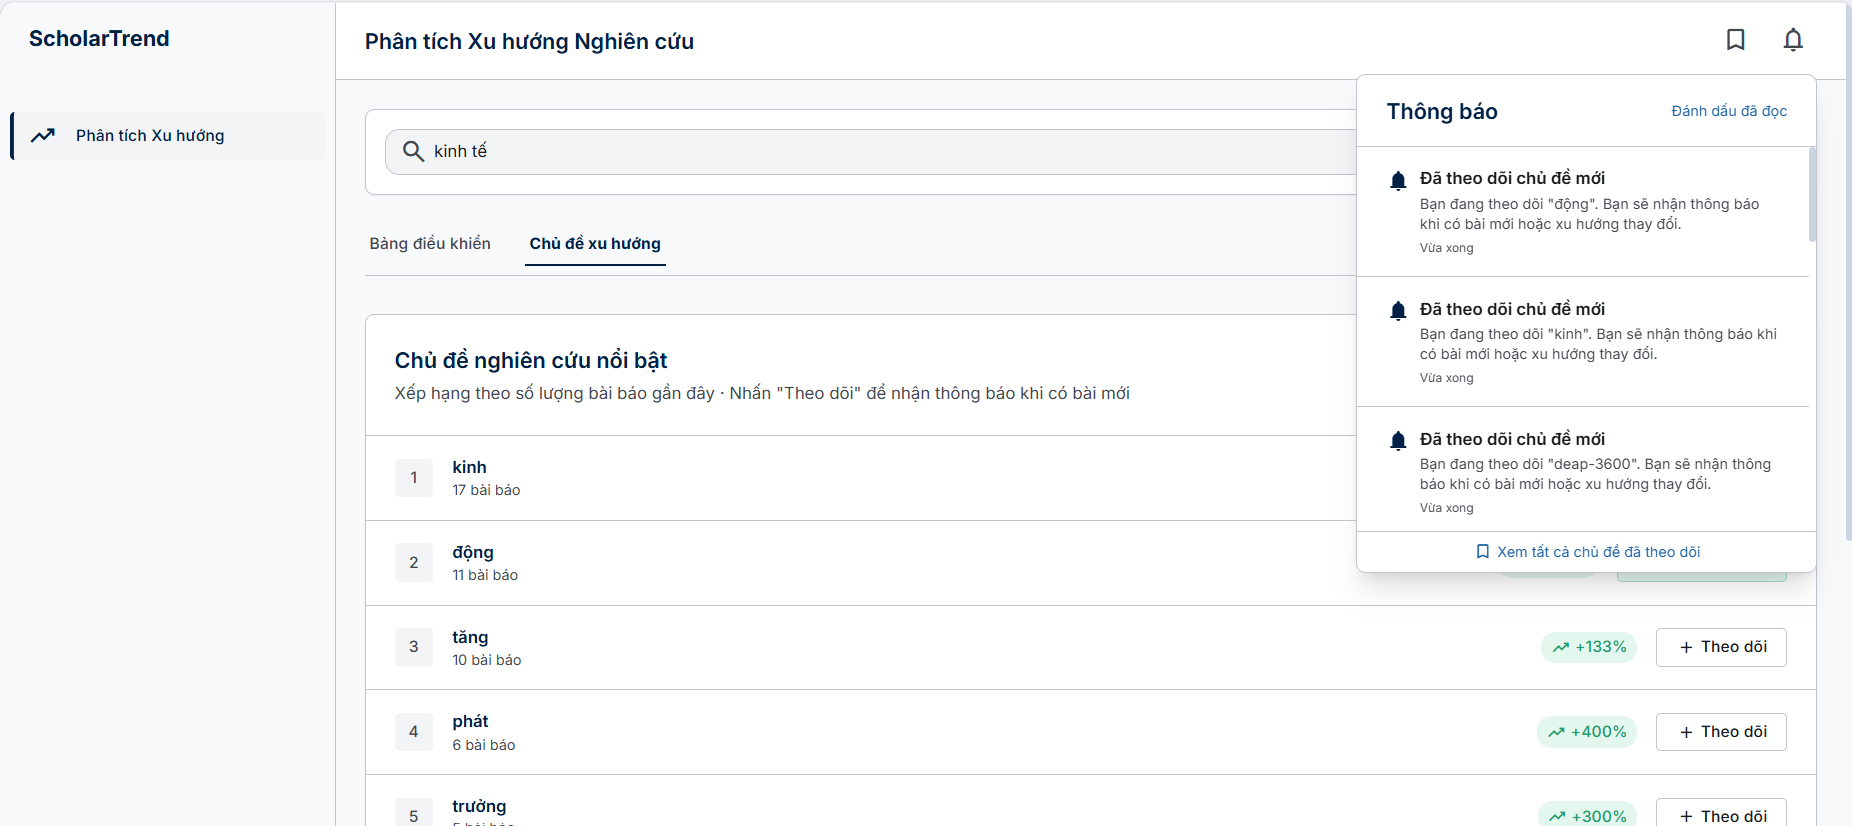
\includegraphics[width=\textwidth]{dadoc.png}

	\label{fig:erd}
\end{figure}
\subsubsection{Admin - User Management}
\textbf{Role:} Admin

\textbf{Function Trigger:}
The admin opens the Admin page and selects Quan ly
nguoi dung.

\textbf{Function description:}
\begin{itemize}[label=-]
	\item Purpose: Allow the admin to manage user accounts in the system.
	\item Data processing: Retrieve user information from the database and update user status or role.
\end{itemize}

\textbf{Function Details:}
\begin{itemize}[label=-]
    \item Display the list of users.
\end{itemize}
\begin{figure}[H]
    \centering
    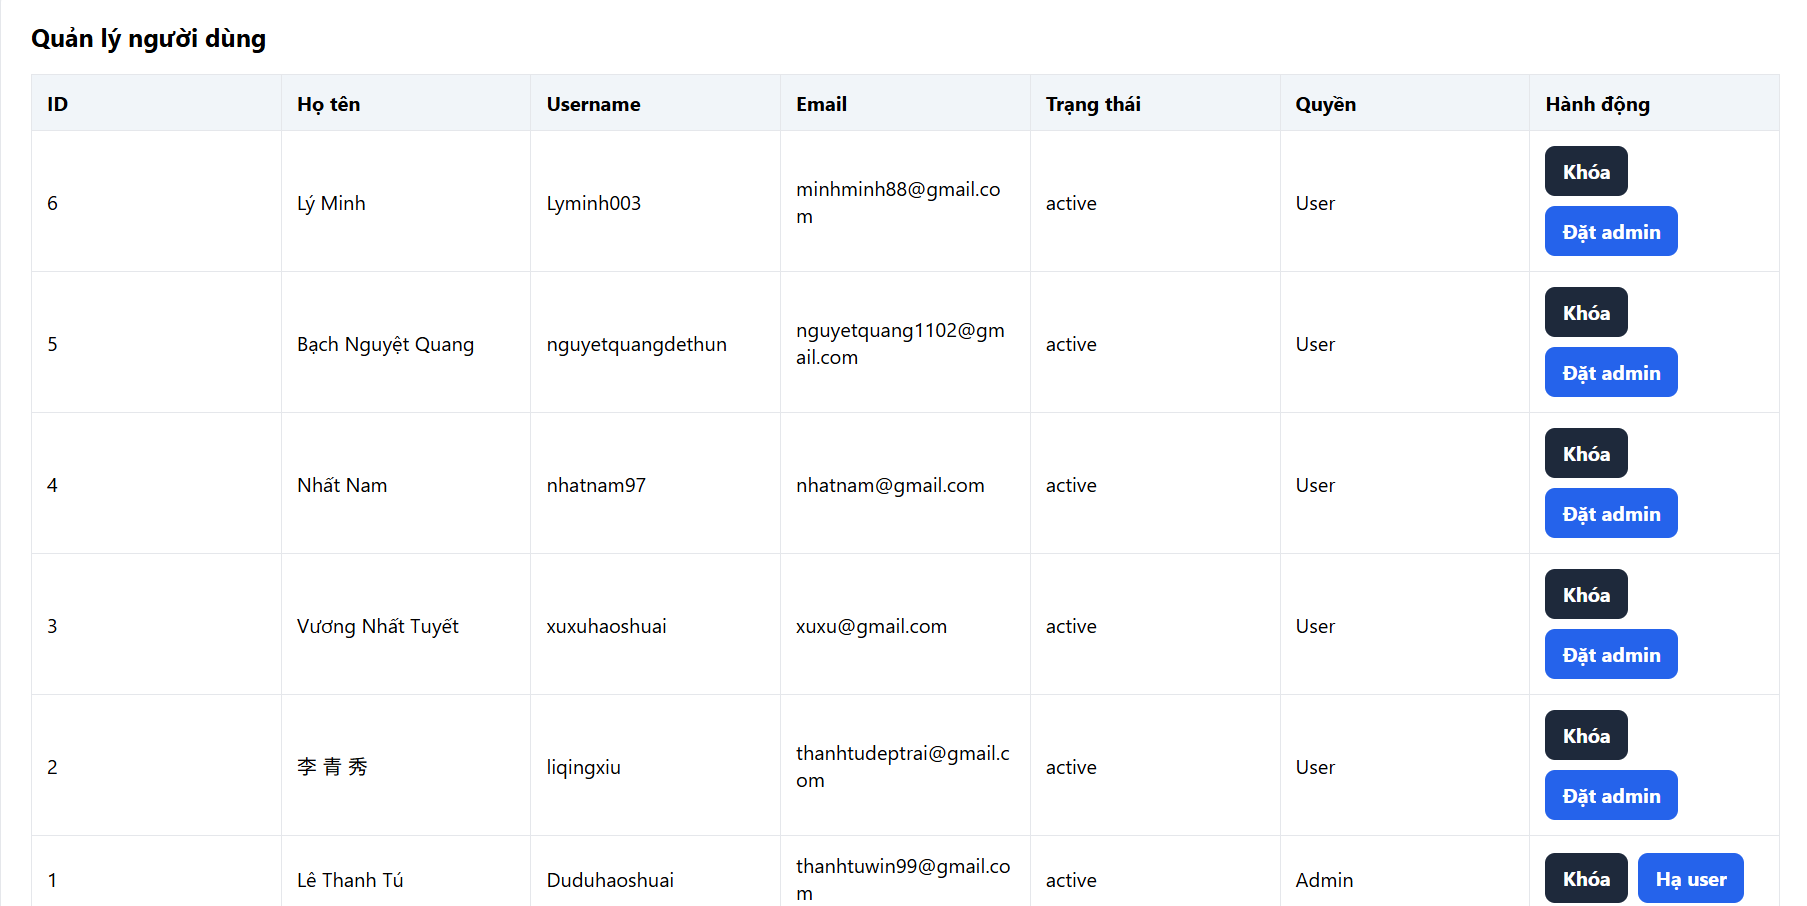
\includegraphics[width=\textwidth]{ad1.png}
   
    \label{fig:admin}
\end{figure}
\begin{itemize}[label=-]
    \item Lock or unlock a user account.
\end{itemize}
\begin{figure}[H]
    \centering
    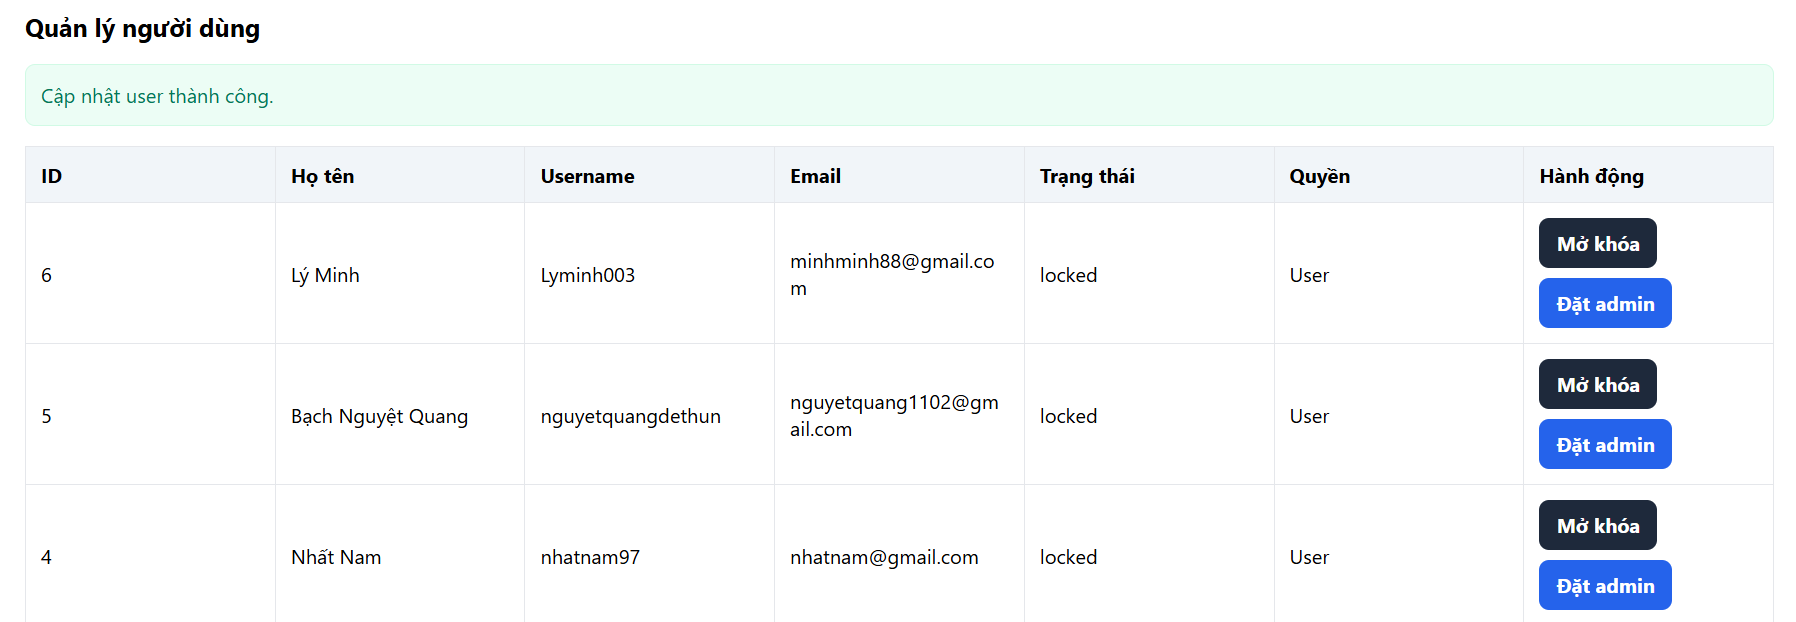
\includegraphics[width=\textwidth]{ad2.png}
  
    \label{fig:admin}
\end{figure}
\begin{itemize}[label=-]
    \item Assign admin role to a user.
\end{itemize}
\begin{figure}[H]
    \centering
    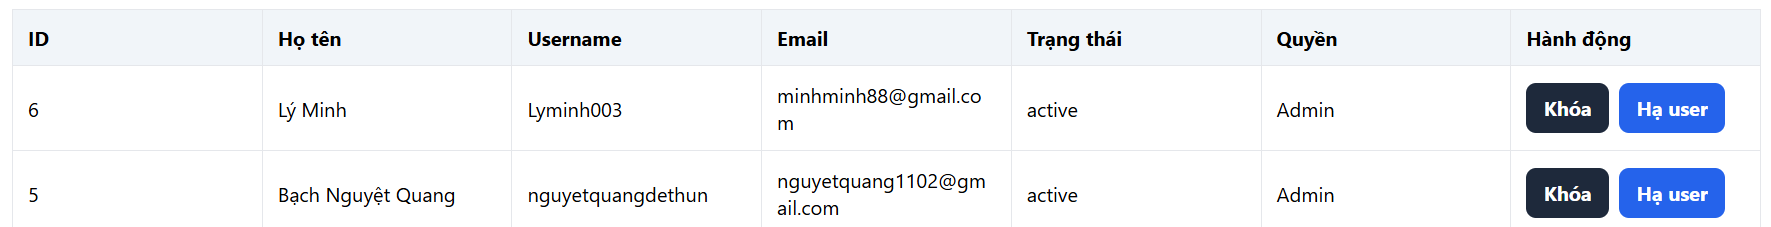
\includegraphics[width=\textwidth]{ad3.png}
   
    \label{fig:admin}
\end{figure}
\begin{itemize}[label=-]
    \item Change an admin account back to a normal user.
\end{itemize}
\begin{figure}[H]
    \centering
    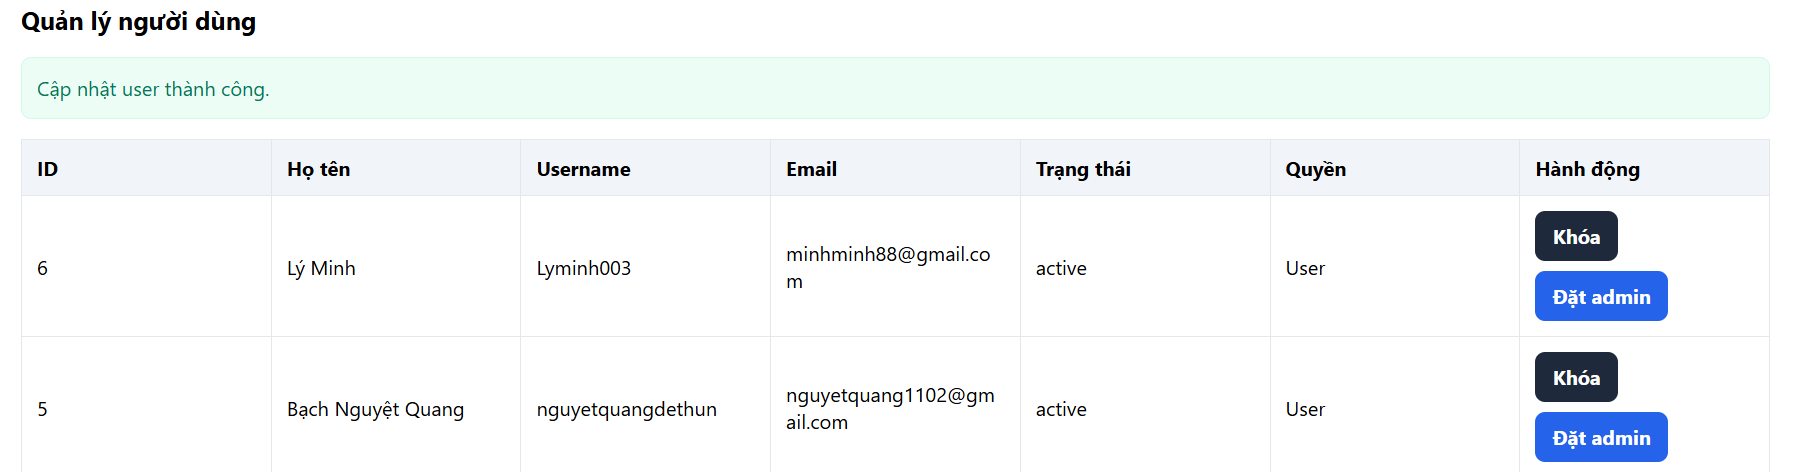
\includegraphics[width=\textwidth]{ad4.png}
  
    \label{fig:admin}
\end{figure}
\begin{itemize}[label=-]
    \item Display a success or error message after each action.
\end{itemize}

\subsubsection{Admin - Topic Management}
\textbf{Role:} Admin
\textbf{Function description:}
\begin{itemize}[label=-]
	\item Purpose: Allow the admin to manage research topics.
	\item Data processing: Add, update, delete, and retrieve topic data from the database.
\end{itemize}
\textbf{Function Details:}
\begin{itemize}[label=-]
    \item Display the list of research topics
\end{itemize}
\begin{figure}[H]
    \centering
    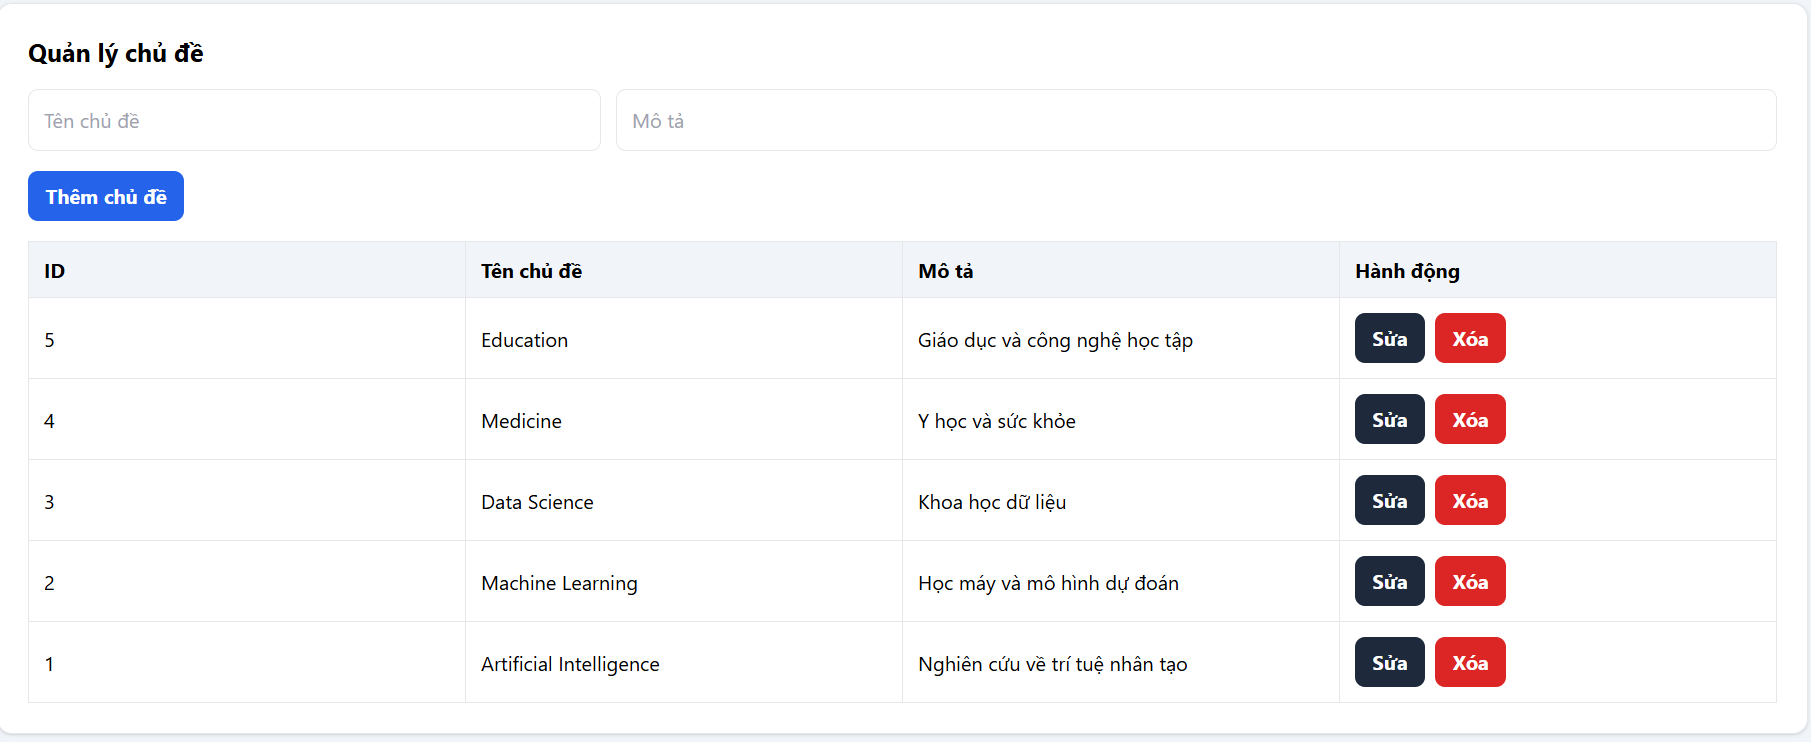
\includegraphics[width=\textwidth]{ad5.png}
  
    \label{fig:admin}
\end{figure}
\begin{itemize}[label=-]
    \item Add a new topic with name and description
\end{itemize}
\begin{figure}[H]
    \centering
    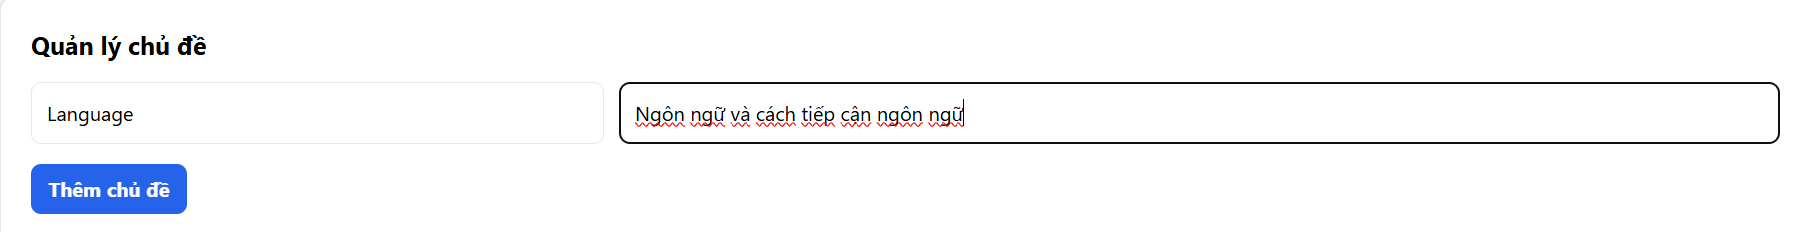
\includegraphics[width=\textwidth]{ad6.png}
  
    \label{fig:admin}
\end{figure}
\begin{itemize}[label=-]
    \item Edit an existing topic
\end{itemize}
\begin{figure}[H]
    \centering
    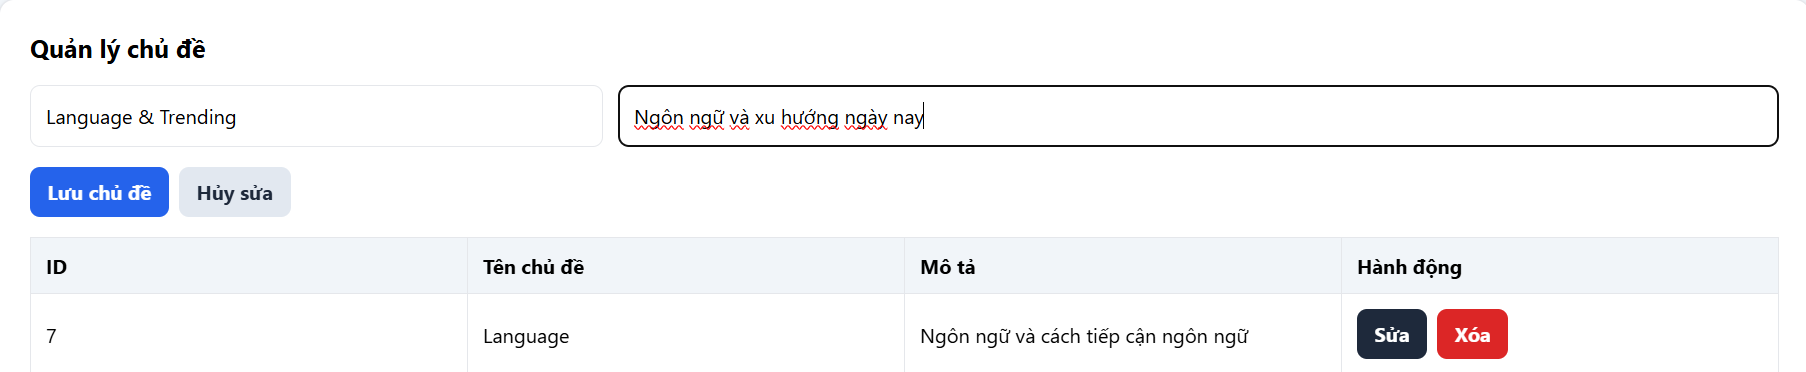
\includegraphics[width=\textwidth]{ad7.png}
   
    \label{fig:admin}
\end{figure}
\begin{itemize}[label=-]
    \item Delete a topic
\end{itemize}
\begin{figure}[H]
	\centering
    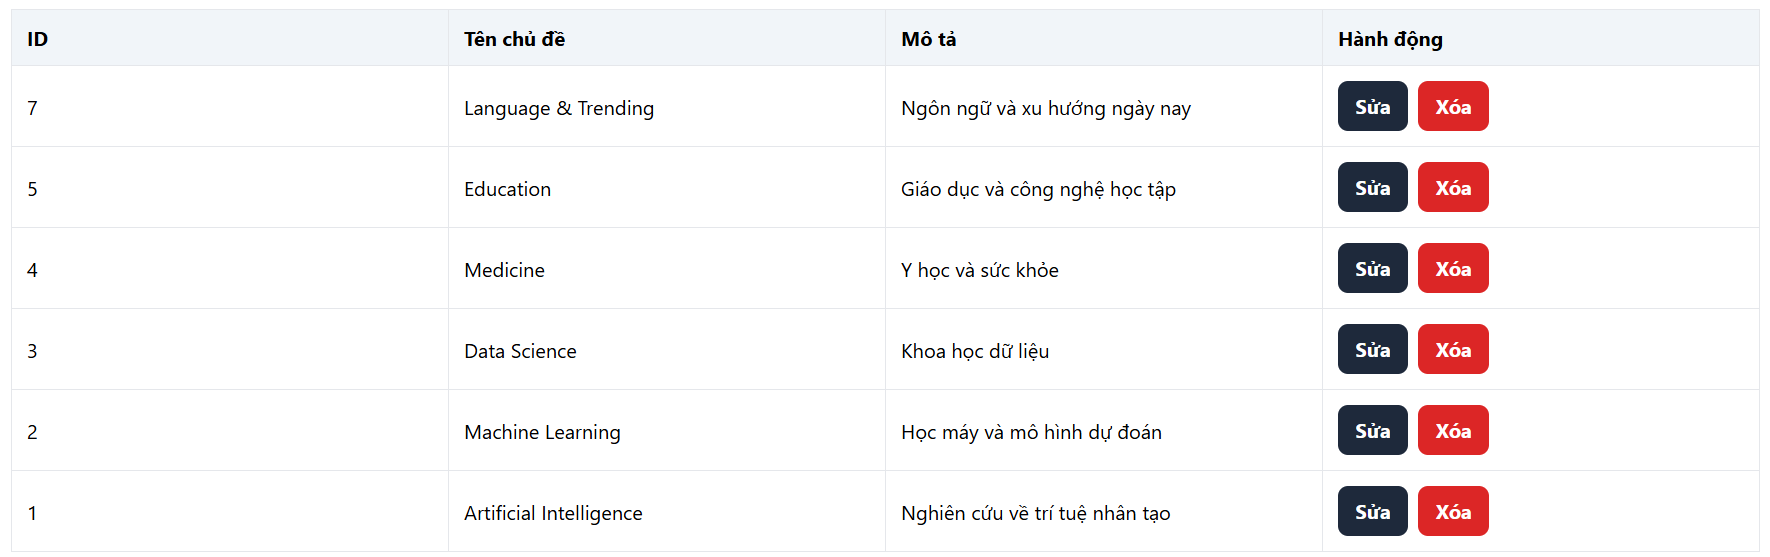
\includegraphics[width=\textwidth]{ad8.png}
  
    \label{fig:admin}
\end{figure}
\begin{figure}[H]
	\centering
    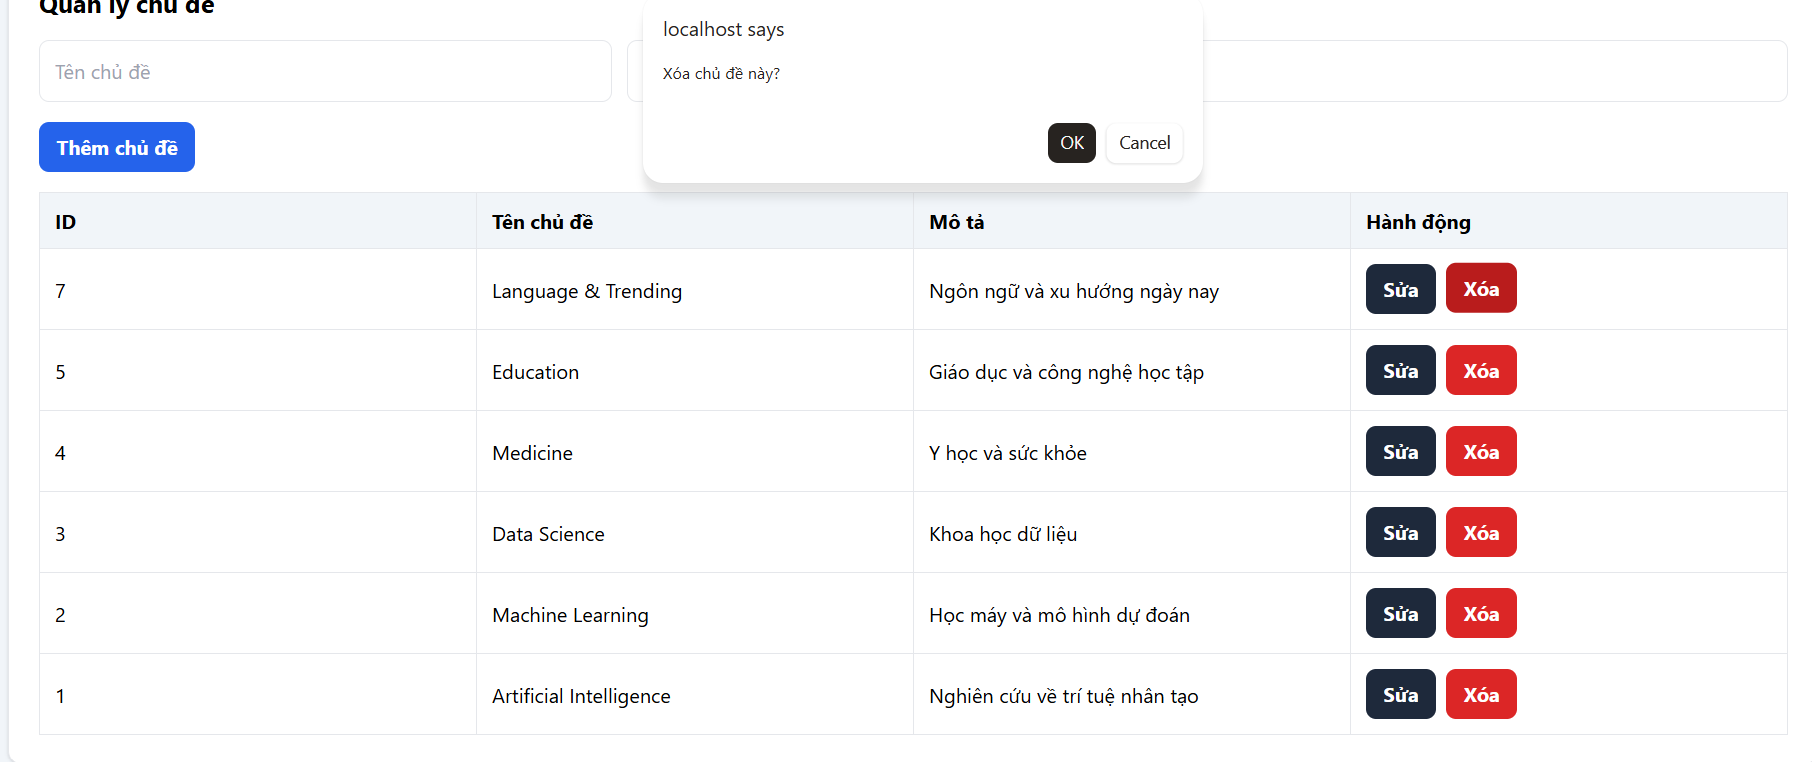
\includegraphics[width=\textwidth]{ad9.png}

    \label{fig:admin}
\end{figure}
\begin{figure}[H]
	\centering
    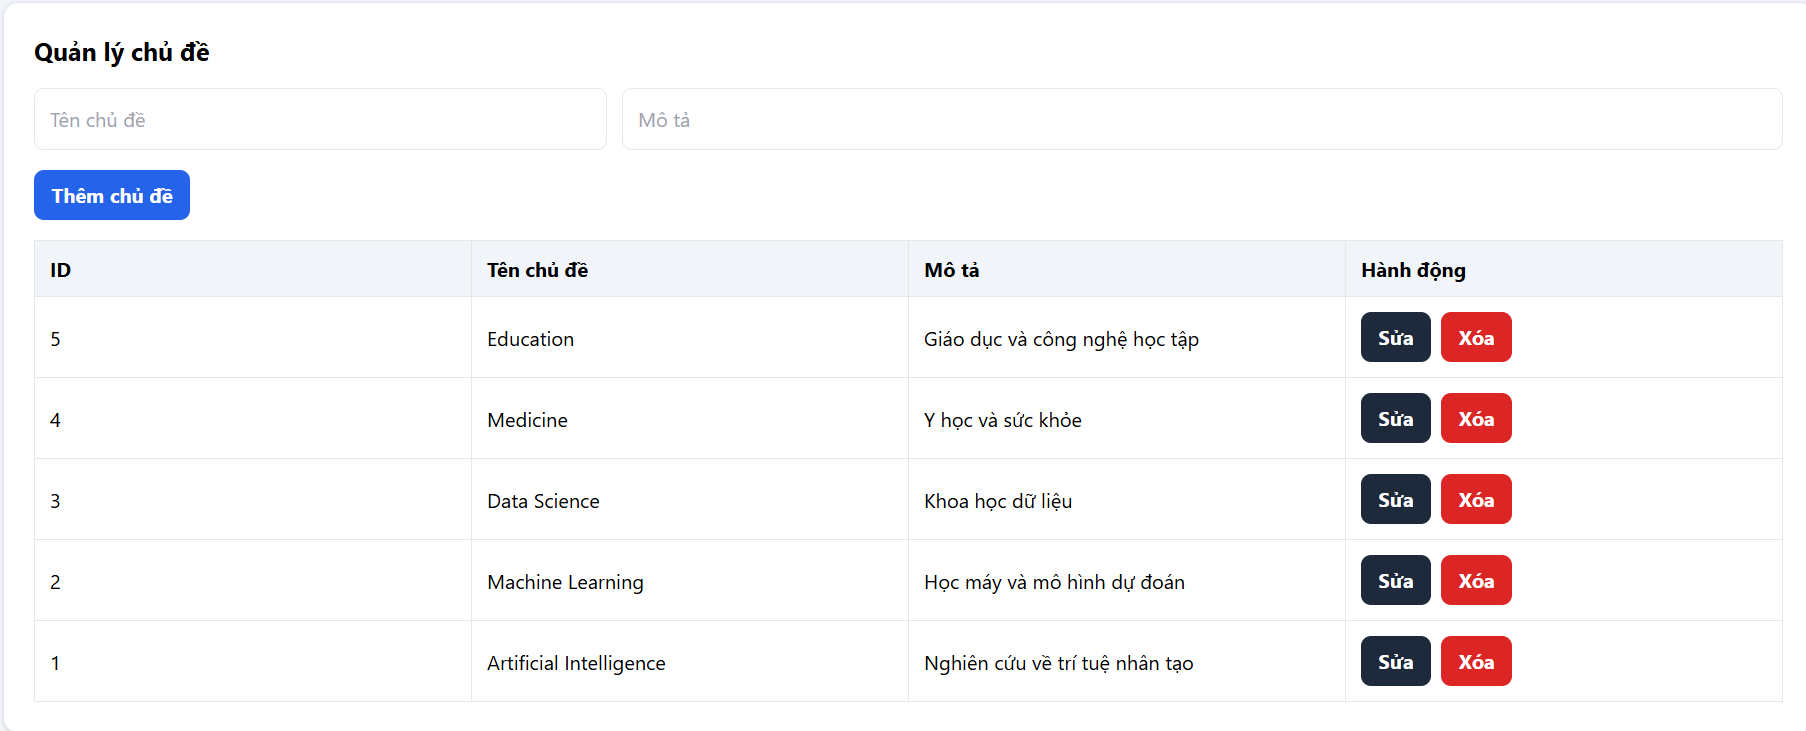
\includegraphics[width=\textwidth]{ad10.png}
    \caption{Admin can delete an existing research topic.}
    \label{fig:admin}
\end{figure}
\begin{itemize}[label=-]
    \item Update the topic list after each action
\end{itemize}
\begin{figure}[H]
	\centering
    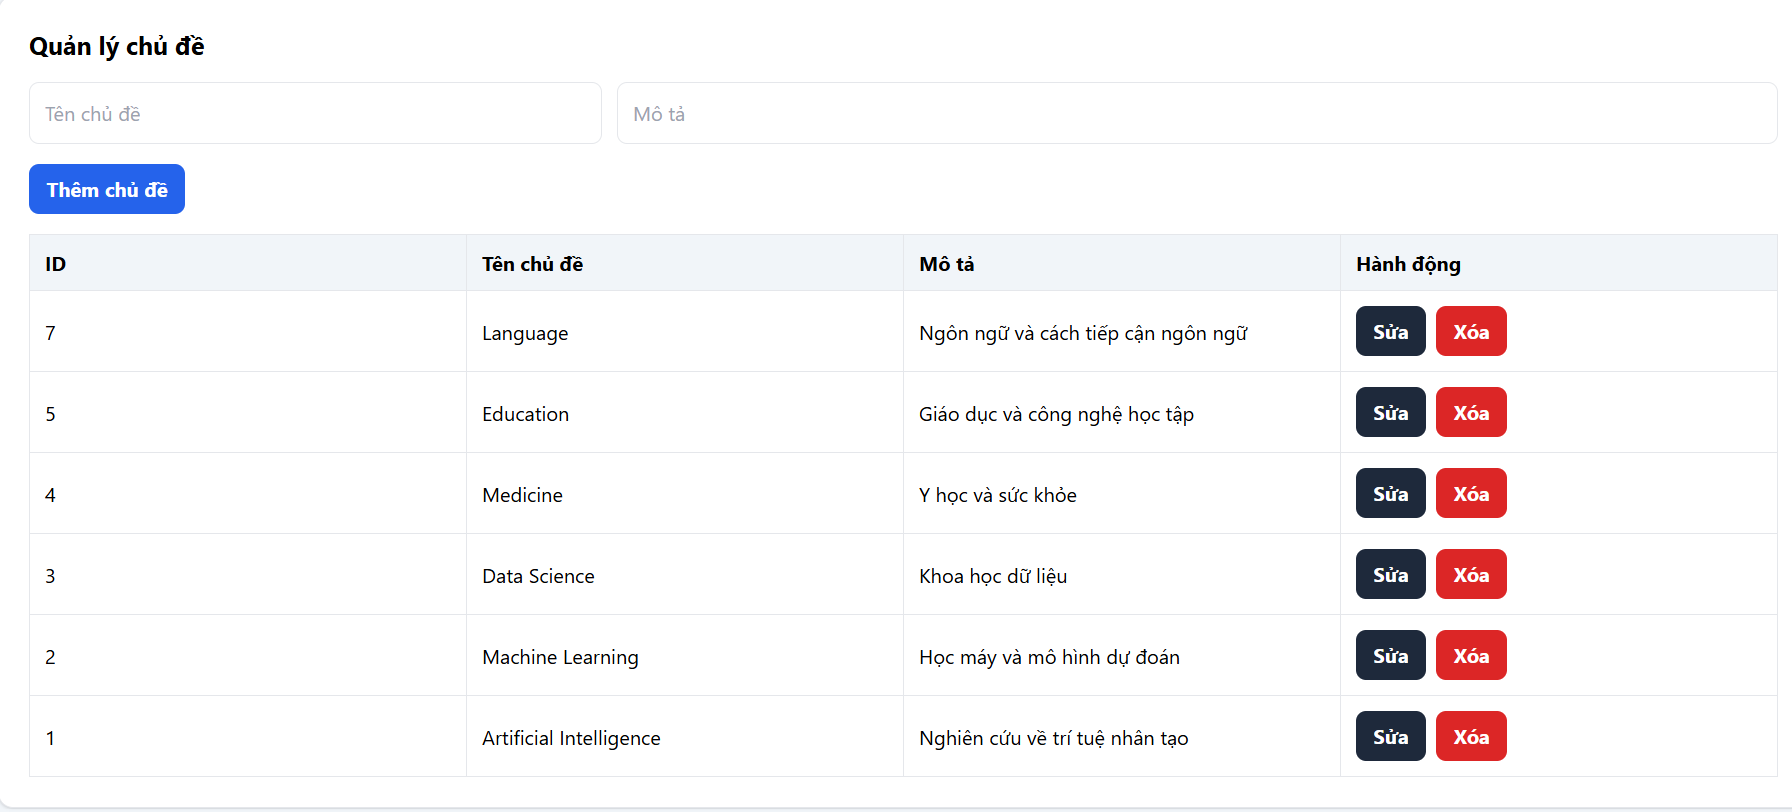
\includegraphics[width=\textwidth]{ad11.png}
   
    \label{fig:admin}
\end{figure}

\subsubsection{Admin - API Source Management}
\textbf{Role:} Admin

\textbf{Function trigger:}
The admin opens the Admin page and selects Quan ly nguon API.

\textbf{Function description:}
\begin{itemize}[label=-]
    \item Purpose: Allow the admin to manage external API sources used by the system.
    \item Data processing: Store and update API source information in the database.
\end{itemize}
\textbf{Function Details:}
\begin{itemize}[label=-]
    \item Display the list of API sources.
\end{itemize}
\begin{figure}[H]
	\centering
    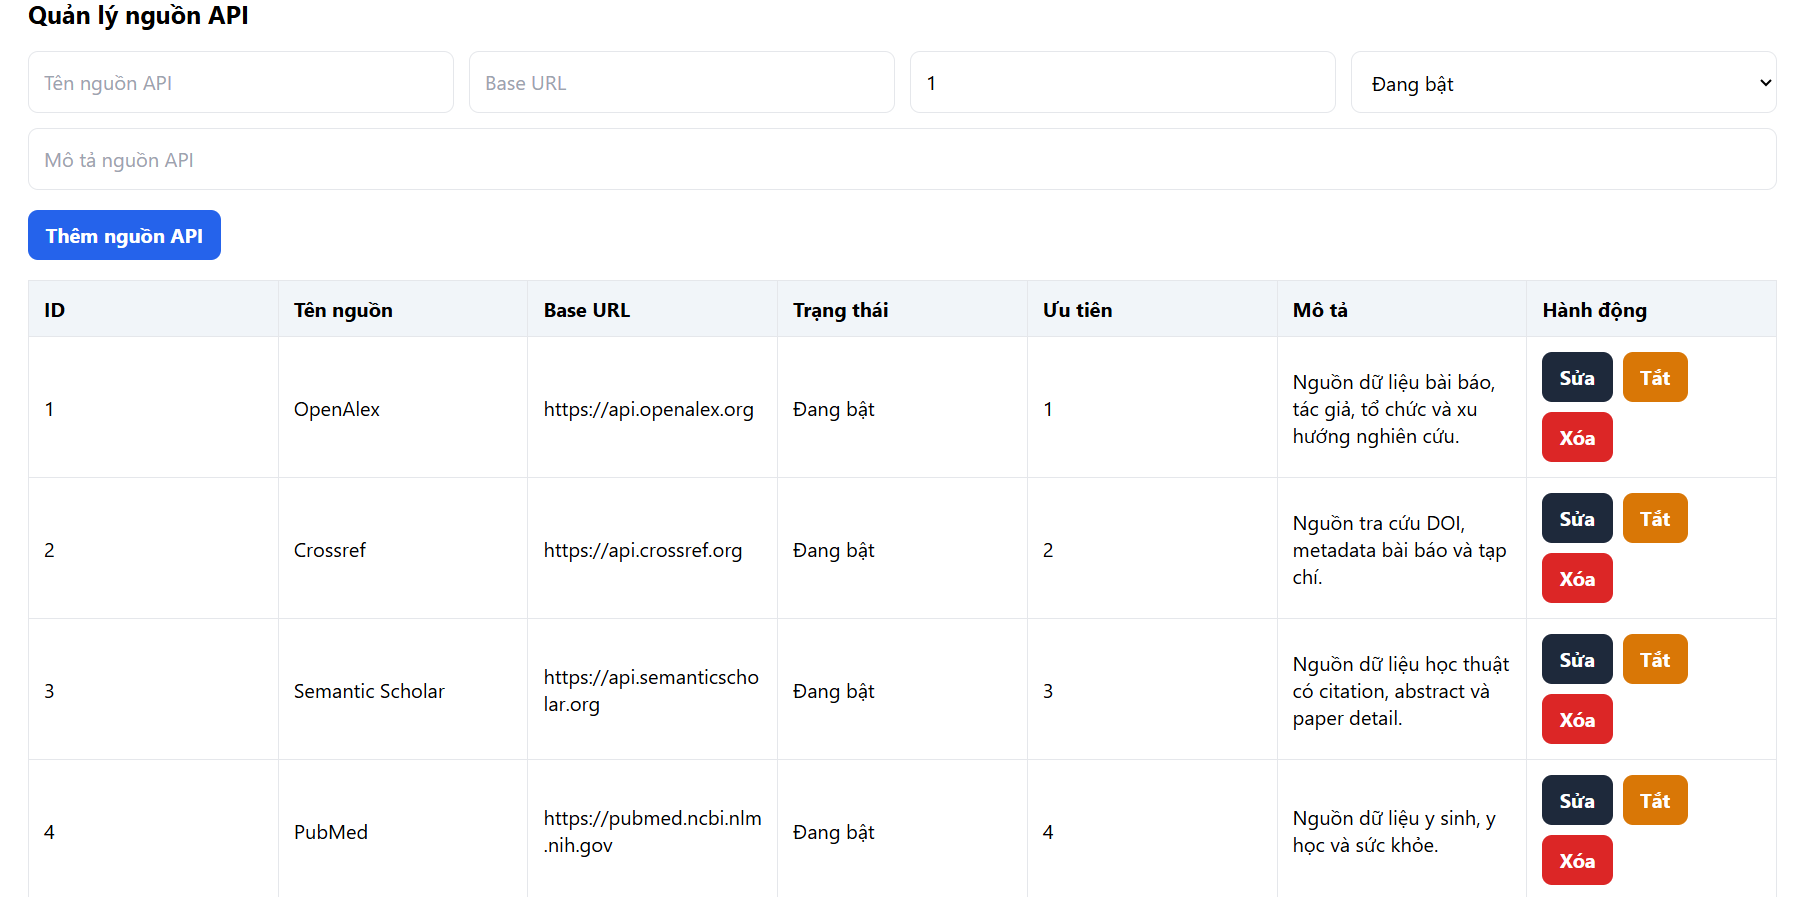
\includegraphics[width=\textwidth]{ad12.png}
   
    \label{fig:admin}
\end{figure}
\begin{itemize}[label=-]
    \item Add a new API source.
\end{itemize}
\begin{itemize}[label=-]
    \item Edit API source name, base URL, status, priority, and description.
\end{itemize}
\begin{figure}[H]
	\centering
    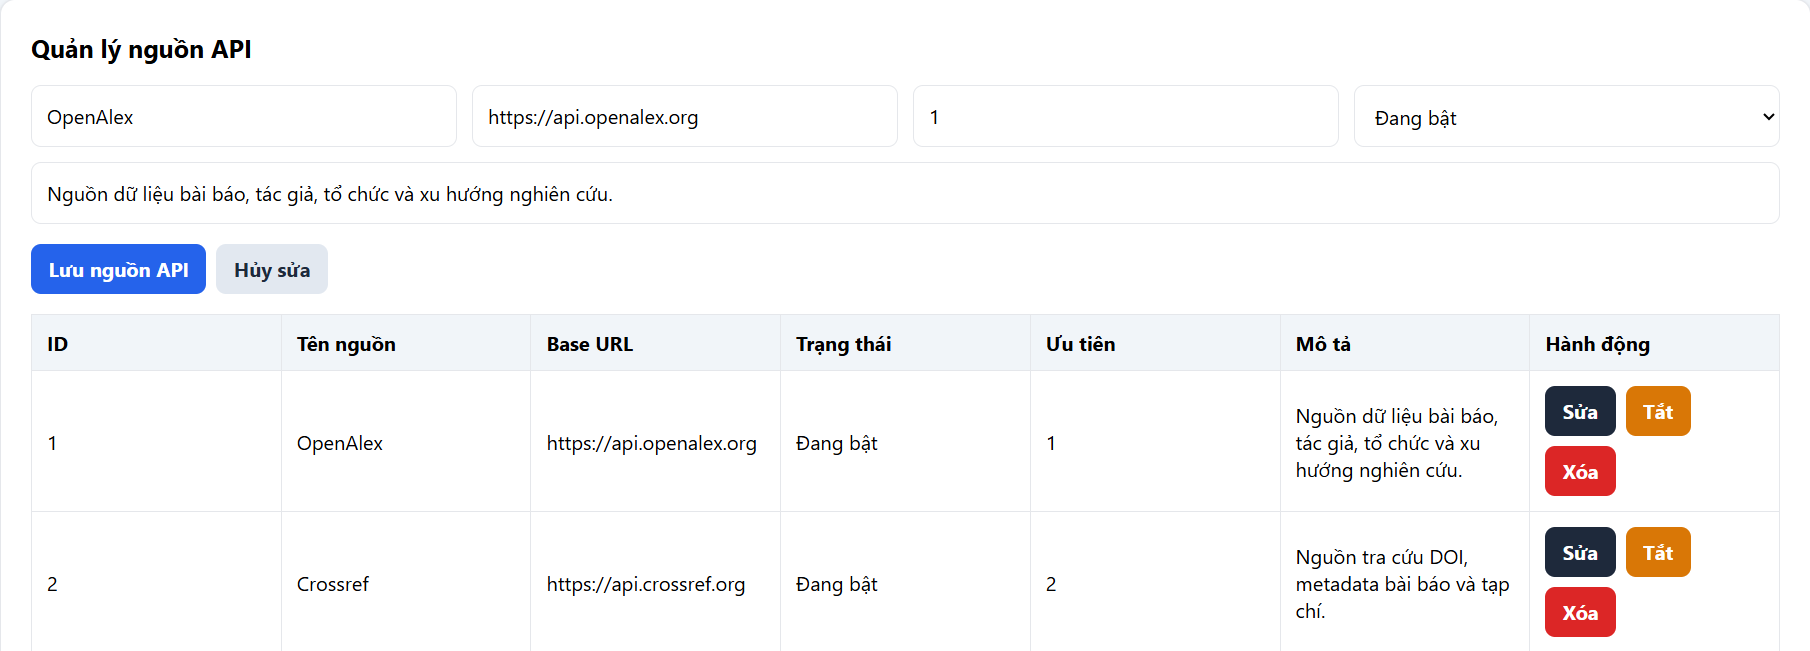
\includegraphics[width=\textwidth]{ad13.png}
   
    \label{fig:admin}
\end{figure}
\begin{itemize}[label=-]
    \item Enable or disable an API source.
\end{itemize}
\begin{figure}[H]
	\centering
    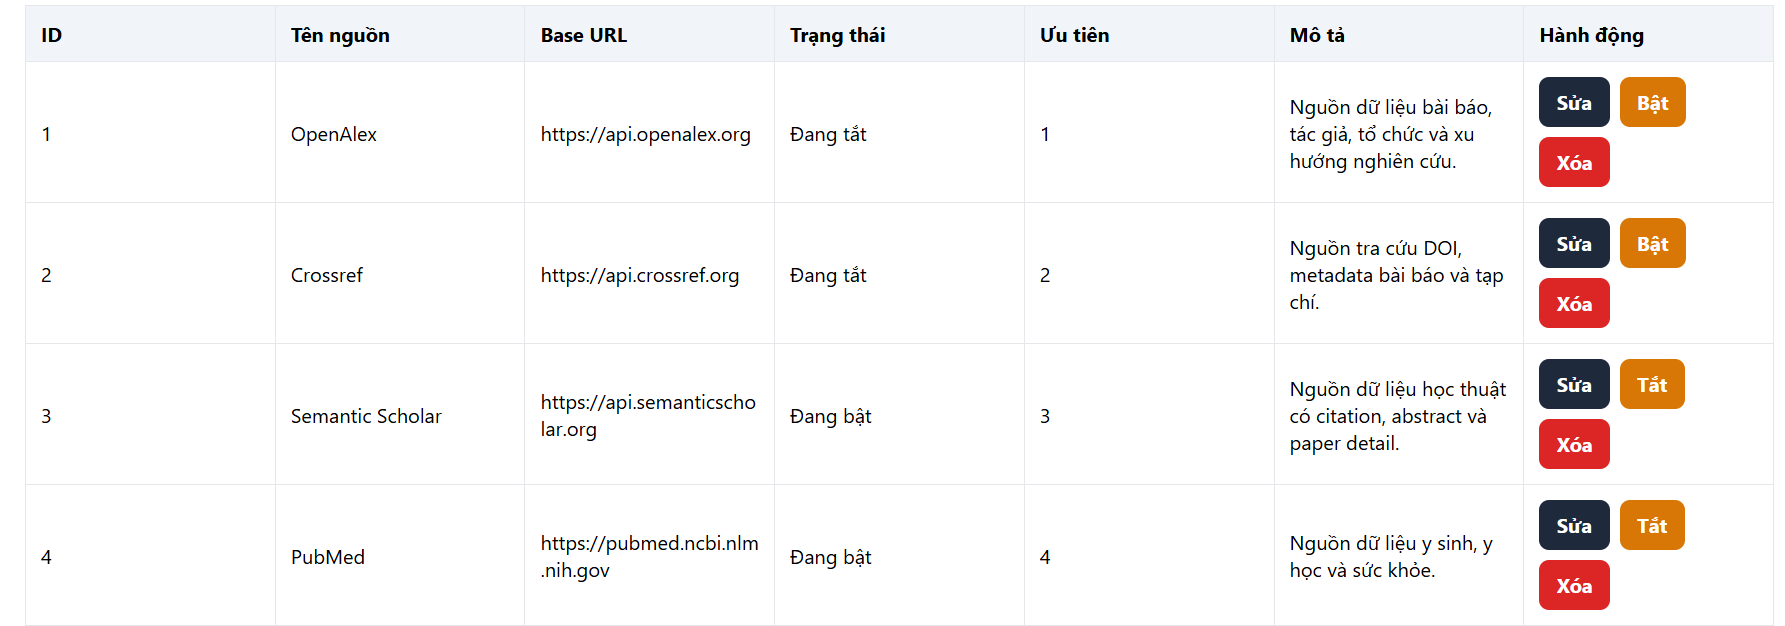
\includegraphics[width=\textwidth]{ad14.png}
  
    \label{fig:admin}
\end{figure}
\begin{itemize}[label=-]
    \item Delete an API source.
\end{itemize}
\begin{figure}[H]
	\centering
    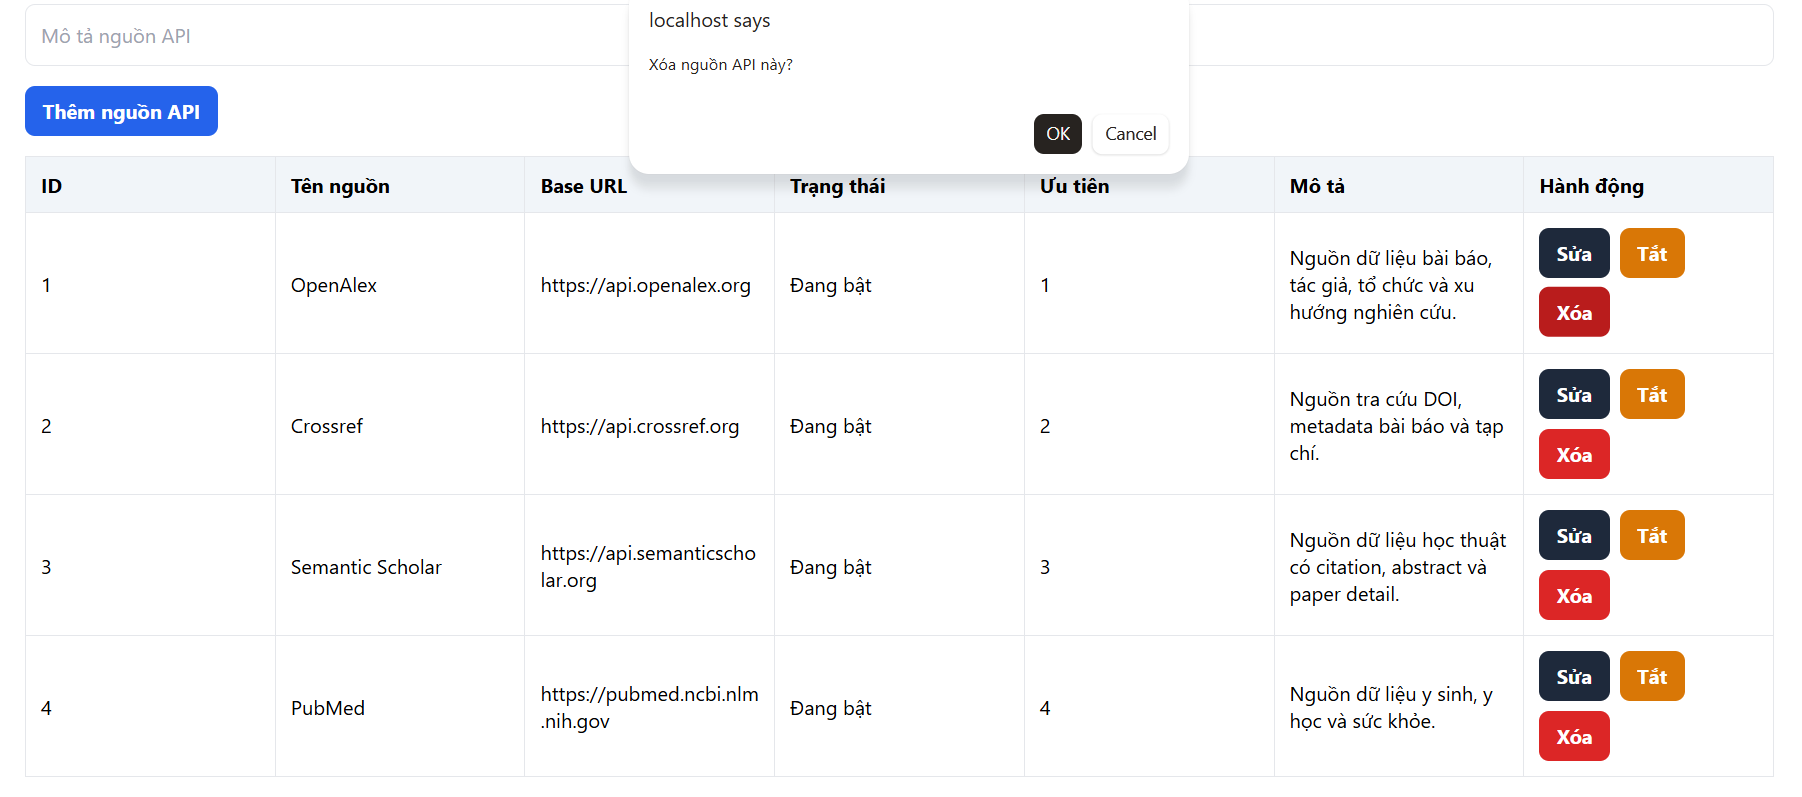
\includegraphics[width=\textwidth]{ad15.png}
   
    \label{fig:admin}
\end{figure}

\subsubsection{Admin - API Data Synchronization}
\textbf{Role:} Admin

\textbf{Function trigger:}
The admin clicks Đong bo hoa in the API synchronization section.

\textbf{Function description:}
\begin{itemize}[label=-]
    \item Purpose: Synchronize data from external APIs into the system.
    \item Data processing: Fetch data from the selected API source, process the returned data, update the research paper database, and save the synchronization log.
\end{itemize}
\textbf{Function Details:}
\begin{itemize}[label=-]
    \item Select an API source.
\end{itemize}
\begin{itemize}[label=-]
    \item Enter a search keyword and the number of records to synchronize.
\end{itemize}
\begin{figure}[H]
	\centering
    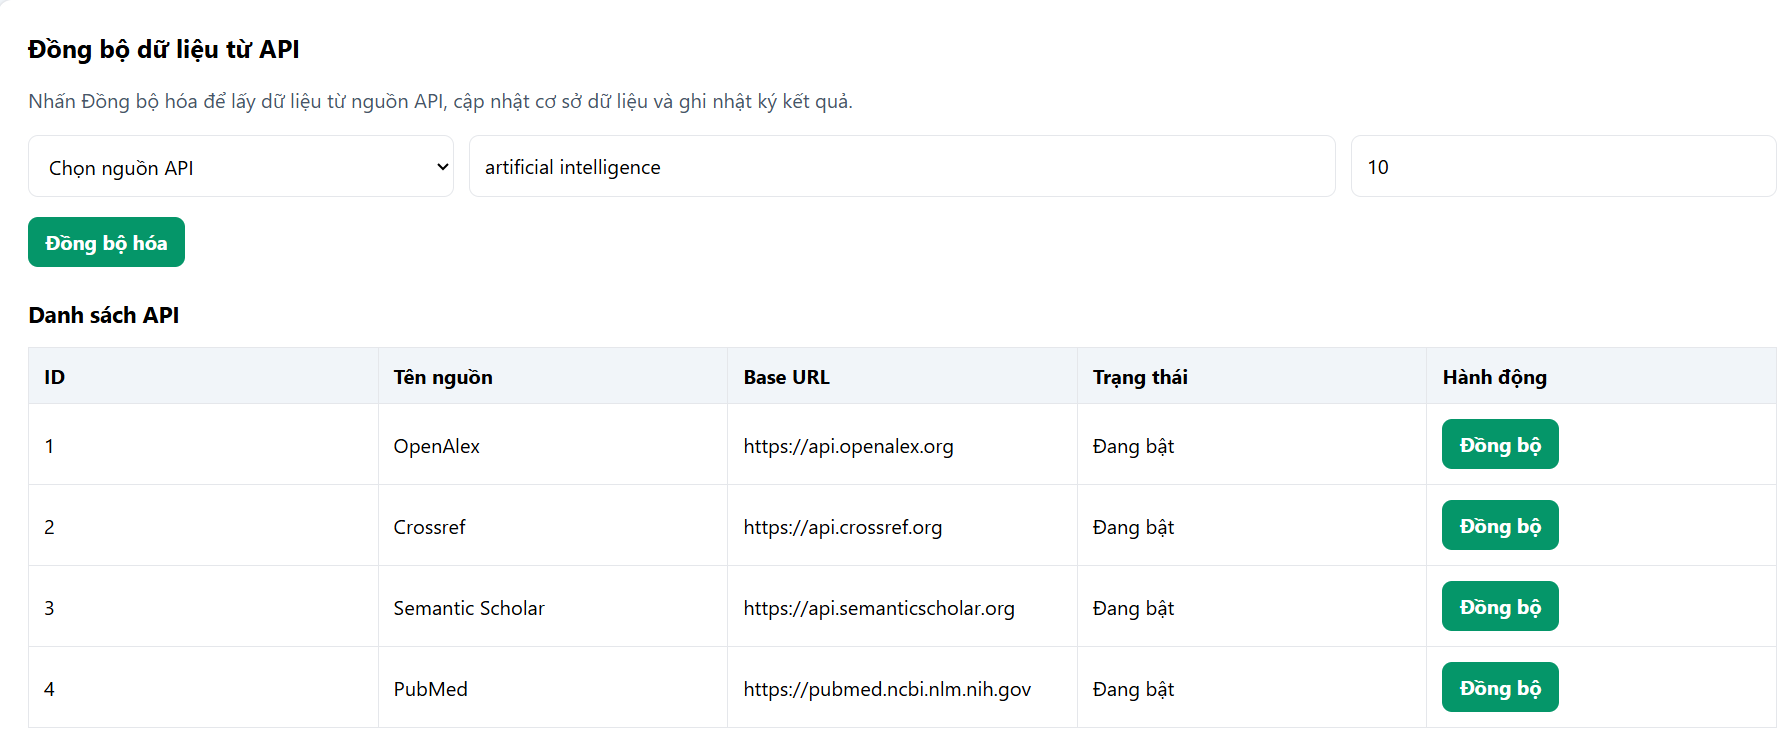
\includegraphics[width=\textwidth]{ad16.png}
  
    \label{fig:admin}
\end{figure}
\begin{itemize}[label=-]
    \item Select an API source.
    \item The system inserts new research papers or updates existing records.
    \item Display synchronization results including fetched, inserted, and updated records.
\end{itemize}
\begin{figure}[H]
	\centering
    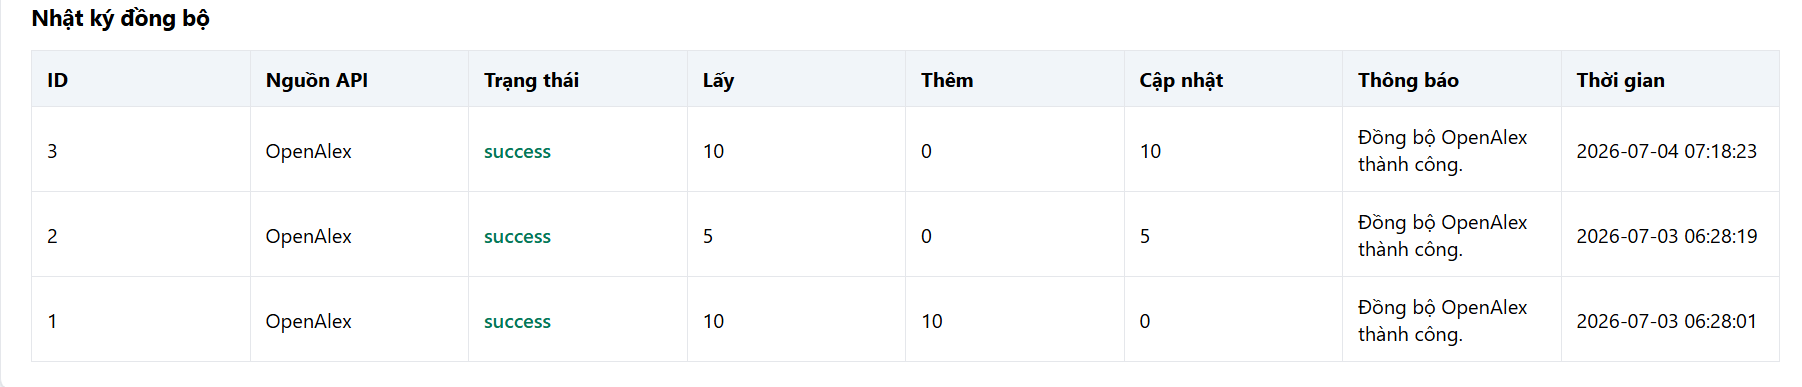
\includegraphics[width=\textwidth]{ad17.png}
   
    \label{fig:admin}
\end{figure}
\begin{itemize}[label=-]
    \item Save the synchronization history in the synchronization log.
\end{itemize}
\begin{figure}[H]
	\centering
    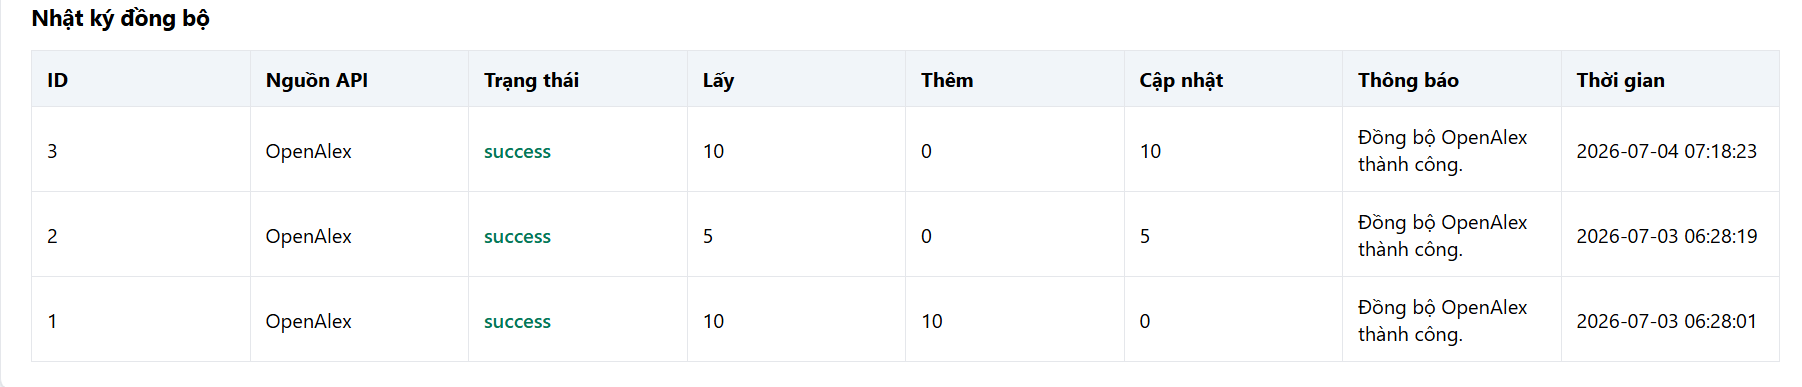
\includegraphics[width=\textwidth]{ad17.png}
    
    \label{fig:admin}
\end{figure}
\subsubsection{Admin - Research Paper Management}
\textbf{Role:} Admin

\textbf{Function trigger:}
The admin opens the Admin page and selects Quan ly bai bao.

\textbf{Function description:}
\begin{itemize}[label=-]
    \item Purpose: Allow the admin to manage research paper data.
    \item Data processing: Add, update, delete, and retrieve research paper information from the database.
\end{itemize}
\textbf{Function Details:}
\begin{itemize}[label=-]
    \item Display the list of research papers.
\end{itemize}
\begin{figure}[H]
	\centering
    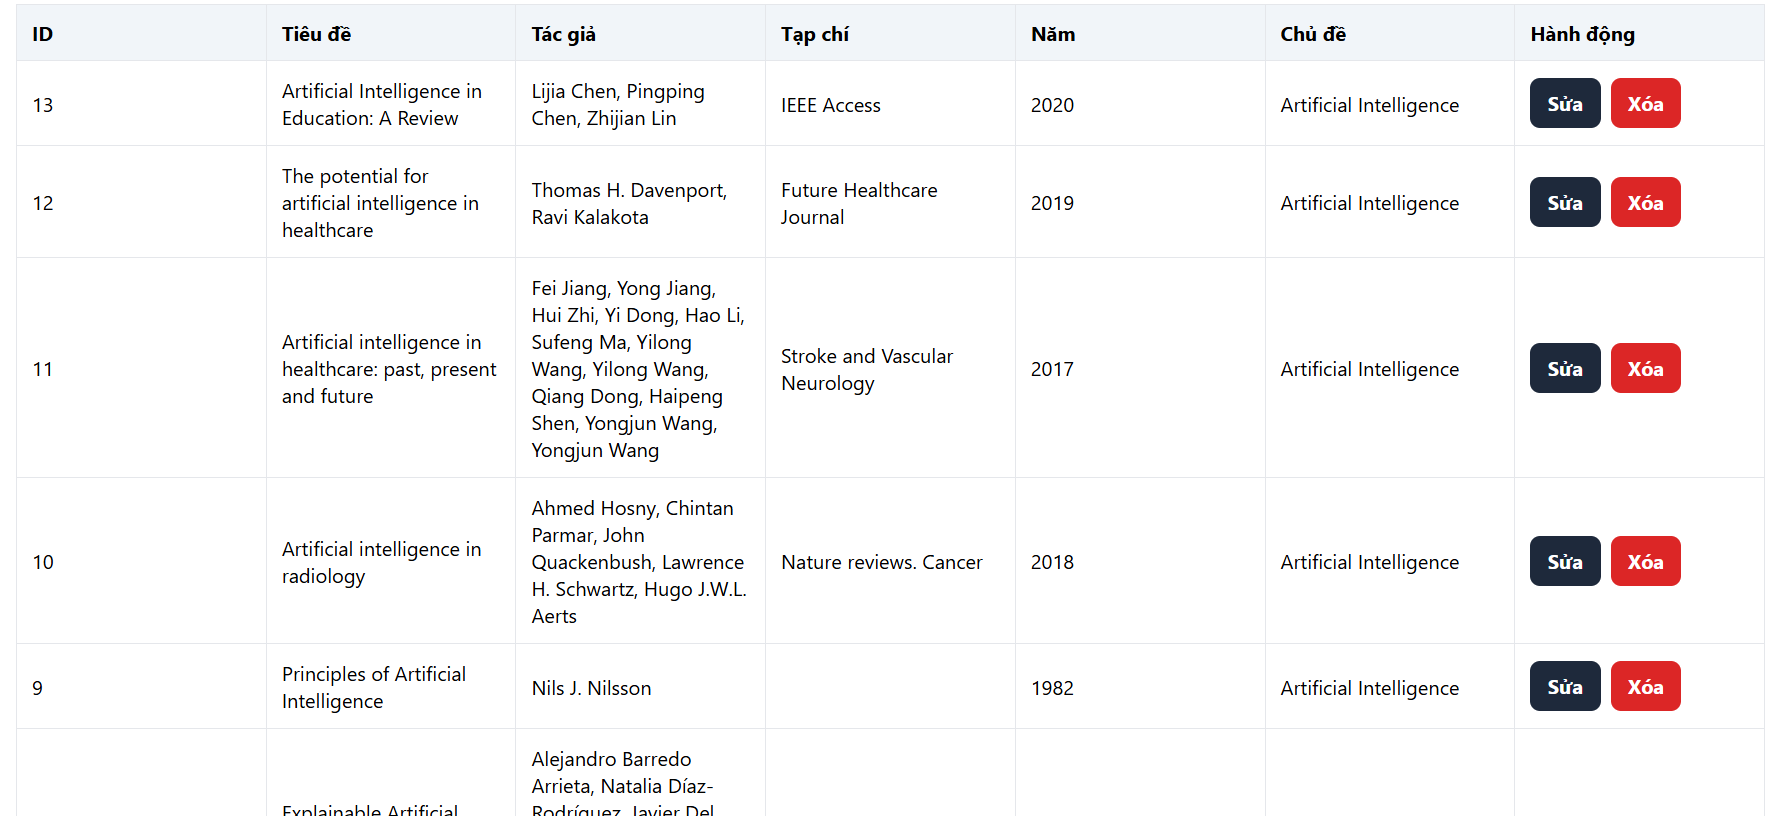
\includegraphics[width=\textwidth]{ad18.png}
   
\end{figure}
\begin{figure}[H]
	\centering
    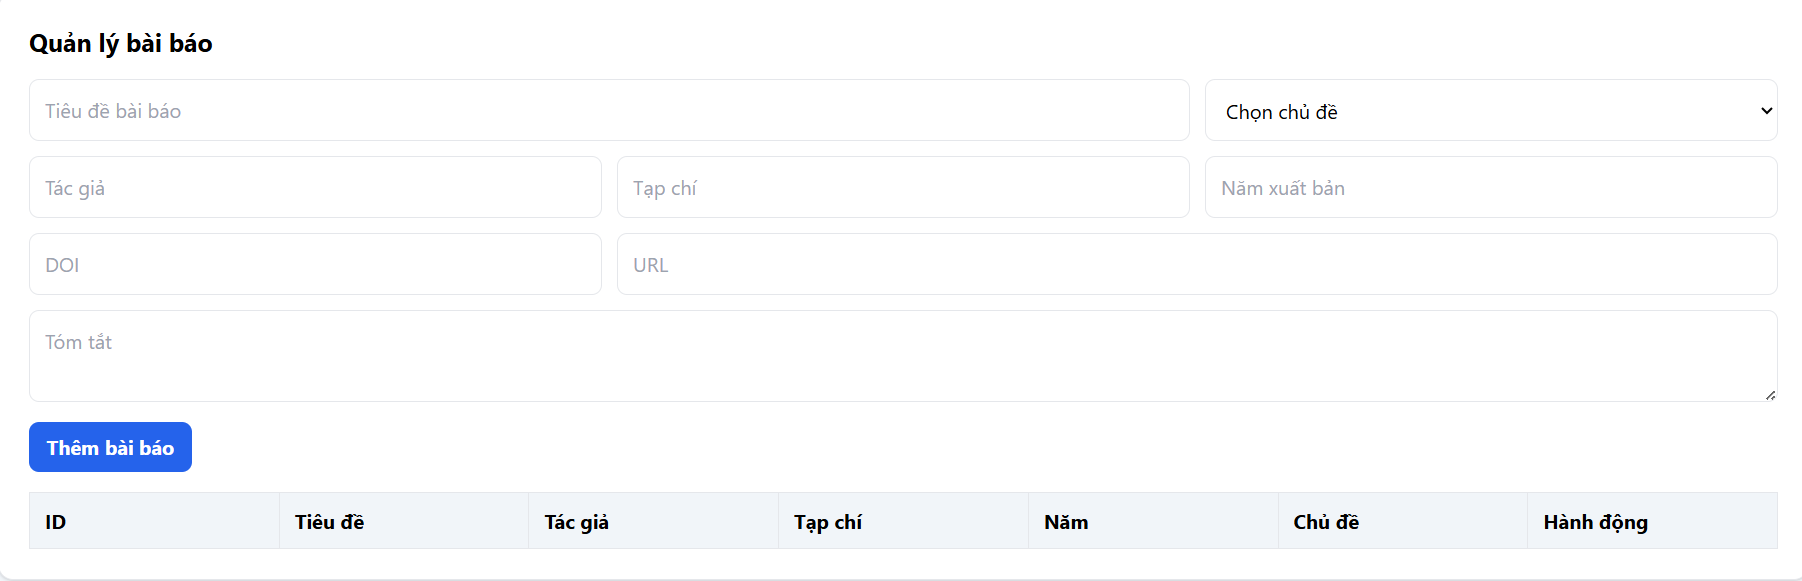
\includegraphics[width=\textwidth]{ad19.png}
   
\end{figure}
\begin{itemize}[label=-]
    \item Add a new research paper.
\end{itemize}
\begin{figure}[H]
	\centering
    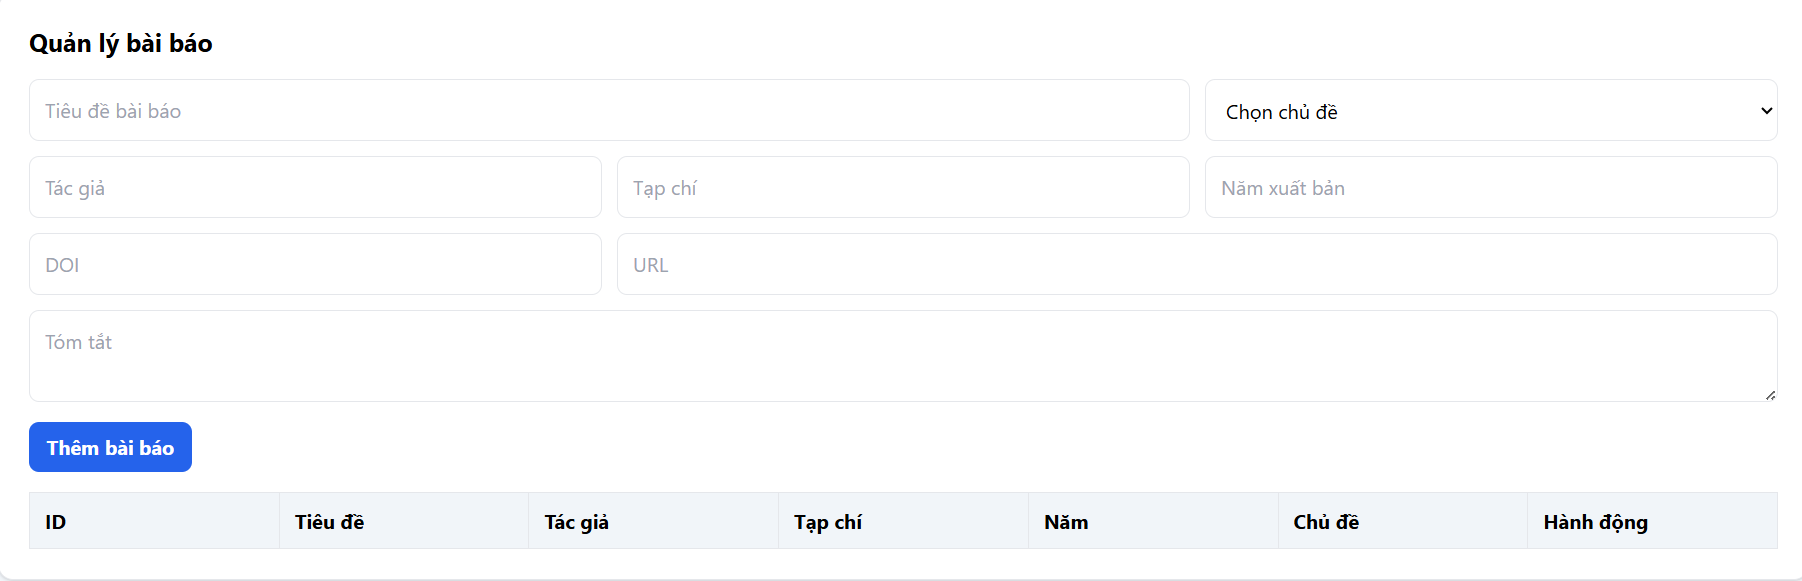
\includegraphics[width=\textwidth]{ad19.png}
   
    \label{fig:admin}
\end{figure}
\begin{itemize}[label=-]
    \item Edit title, authors, journal, publication year, DOI, URL, abstract, and topic.
\end{itemize}
\begin{figure}[H]
	\centering
    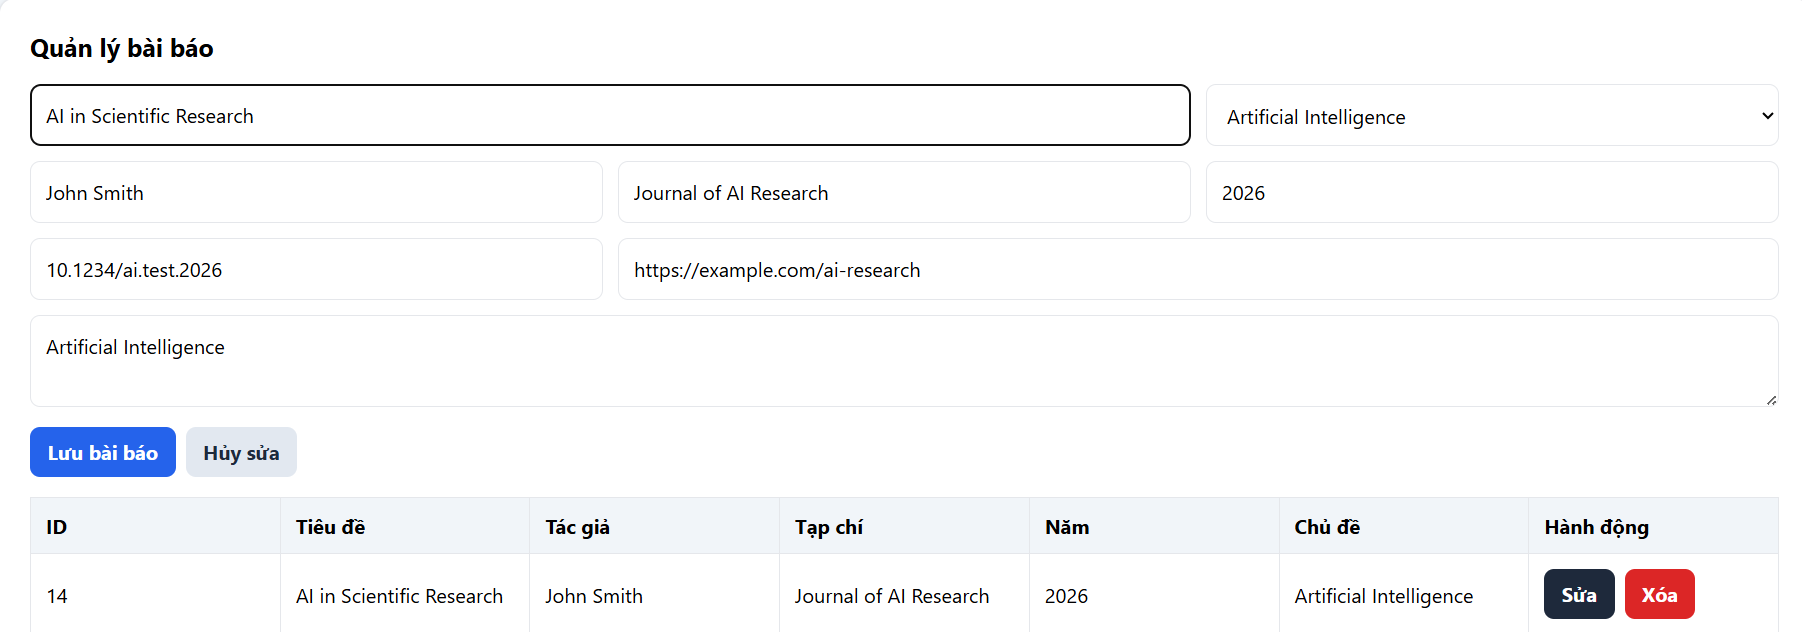
\includegraphics[width=\textwidth]{ad20.png}
   
    \label{fig:admin}
\end{figure}
\begin{itemize}[label=-]
    \item Delete a research paper.
\end{itemize}
\begin{figure}[H]
	\centering
    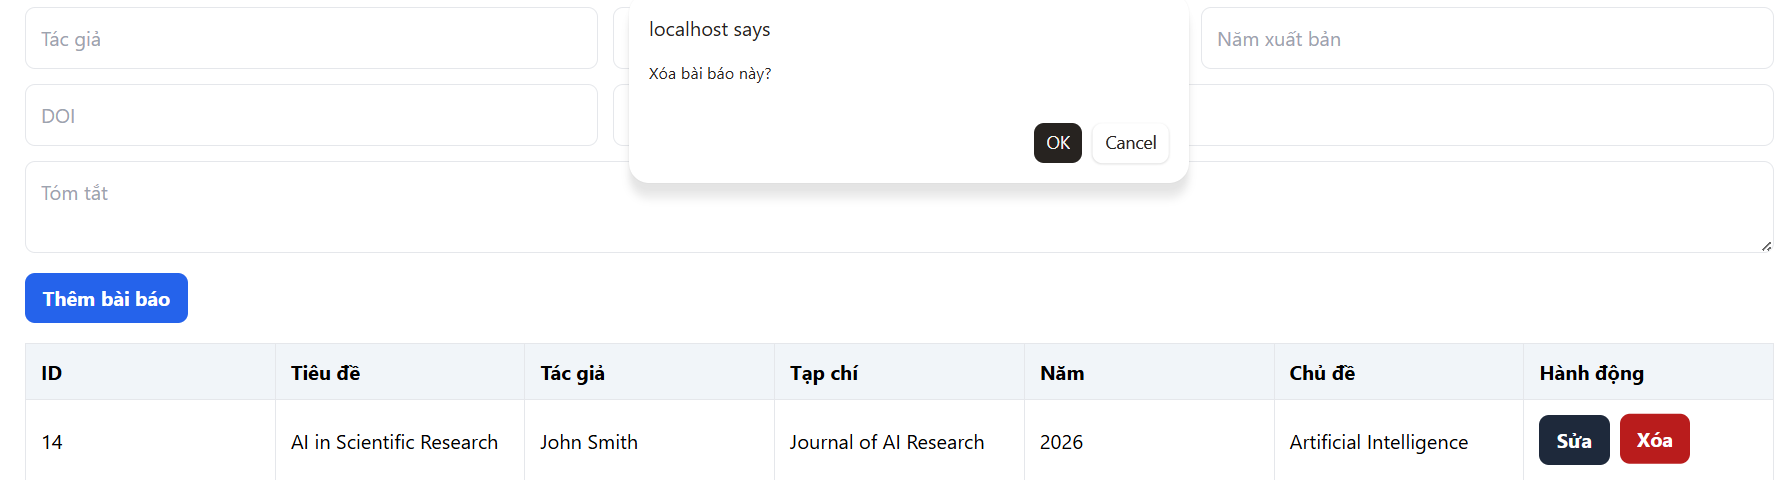
\includegraphics[width=\textwidth]{ad21.png}
   
    \label{fig:admin}
\end{figure}
\begin{itemize}[label=-]
    \item Update the paper list after each action.
\end{itemize}
\begin{figure}[H]
	\centering
    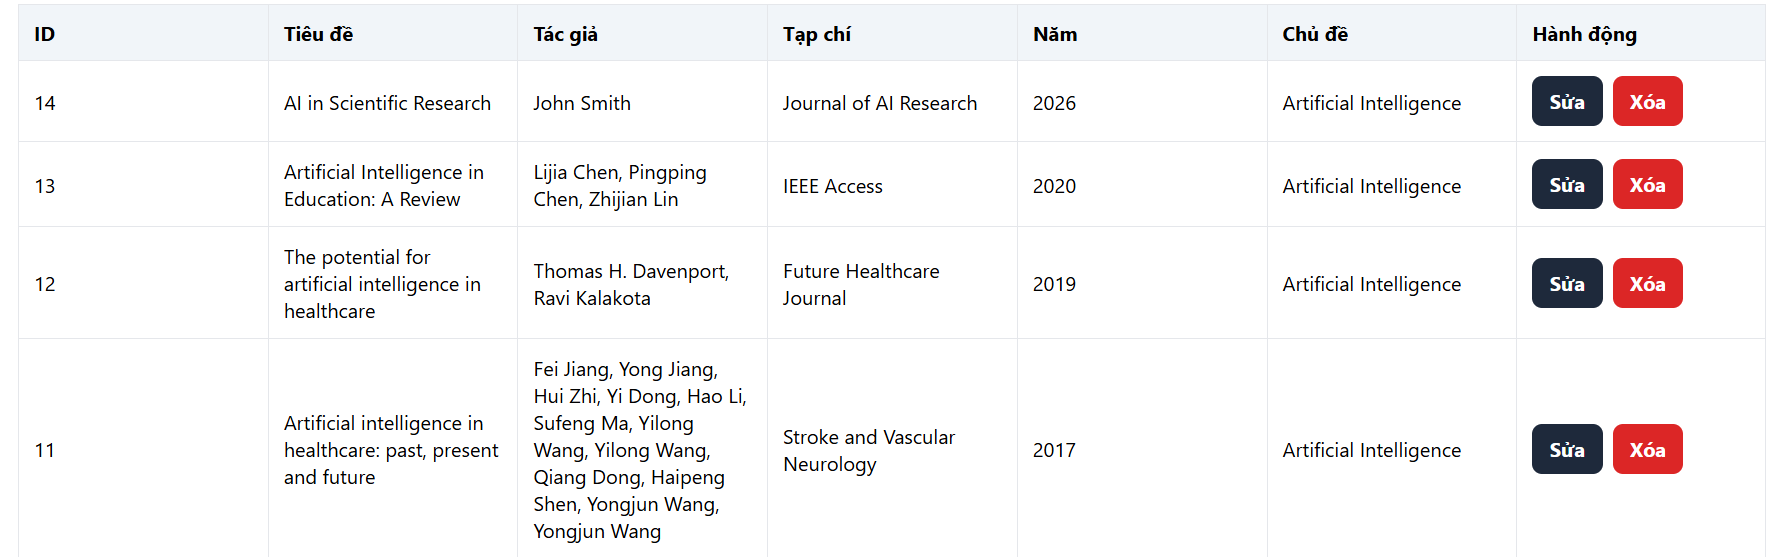
\includegraphics[width=\textwidth]{ad22.png}
   
    \label{fig:admin}
\end{figure}
\subsubsection{Admin - Notification Management}
\textbf{Role:} Admin

\textbf{Function trigger:}
The admin opens the Admin page and selects Quan ly thong bao.

\textbf{Function description:}
\begin{itemize}[label=-]
    \item Purpose: Allow the admin to send and manage notifications for users.
    \item Data processing: Store notification data in the database and retrieve notification history.
\end{itemize}
\textbf{Function Details:}
\begin{itemize}[label=-]
    \item Create a new notification with title, type, link, and content.
\end{itemize}
\begin{figure}[H]
	\centering
    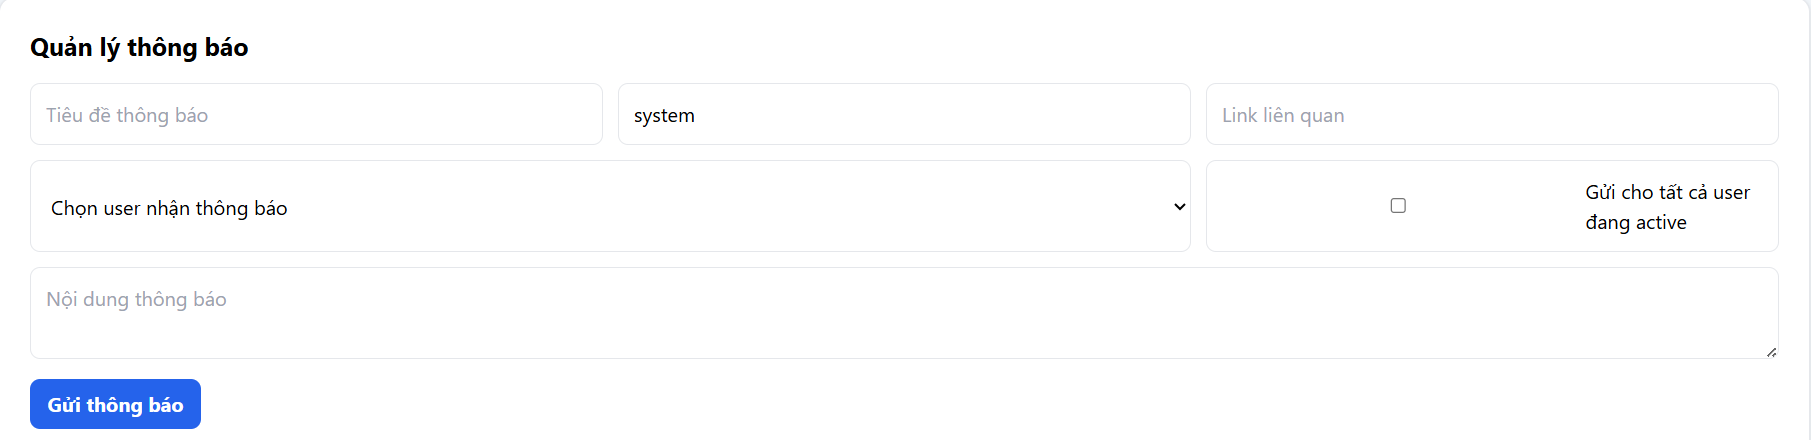
\includegraphics[width=\textwidth]{ad23.png}
   
    \label{fig:admin}
\end{figure}
\begin{itemize}[label=-]
    \item Send a notification to one user or all active users.
    \item Display the list of sent notifications.
\end{itemize}
\begin{figure}[H]
	\centering
    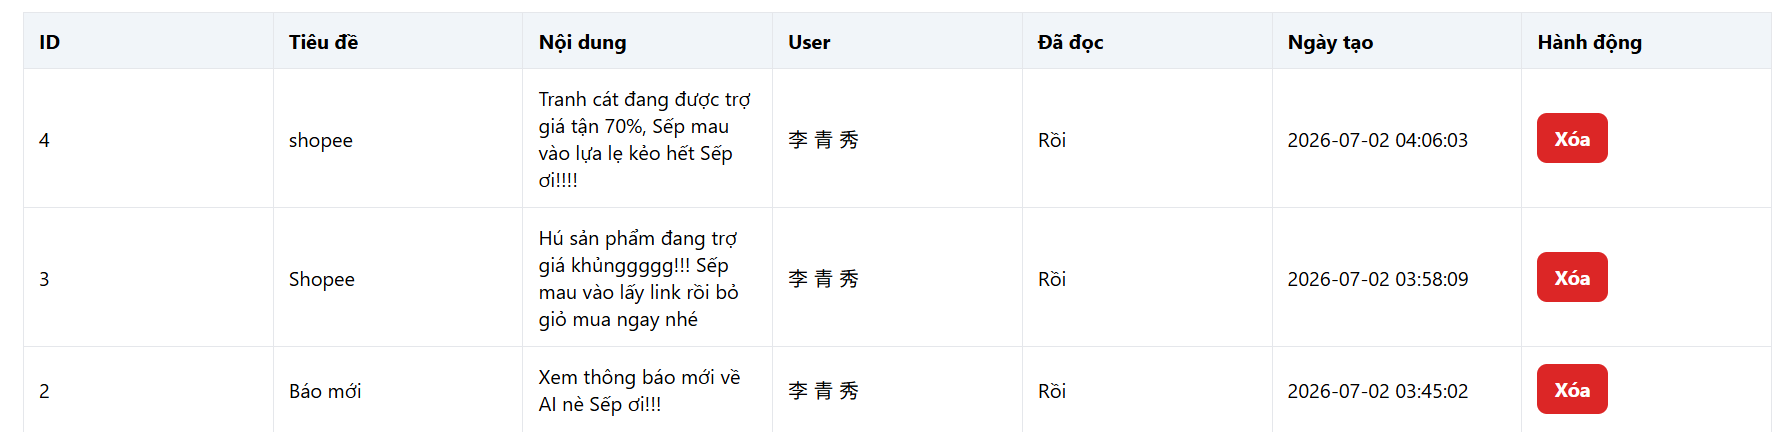
\includegraphics[width=\textwidth]{ad24.png}
    
    \label{fig:admin}
\end{figure}
\begin{itemize}[label=-]
    \item Delete a notification.
\end{itemize}
\begin{figure}[H]
	\centering
    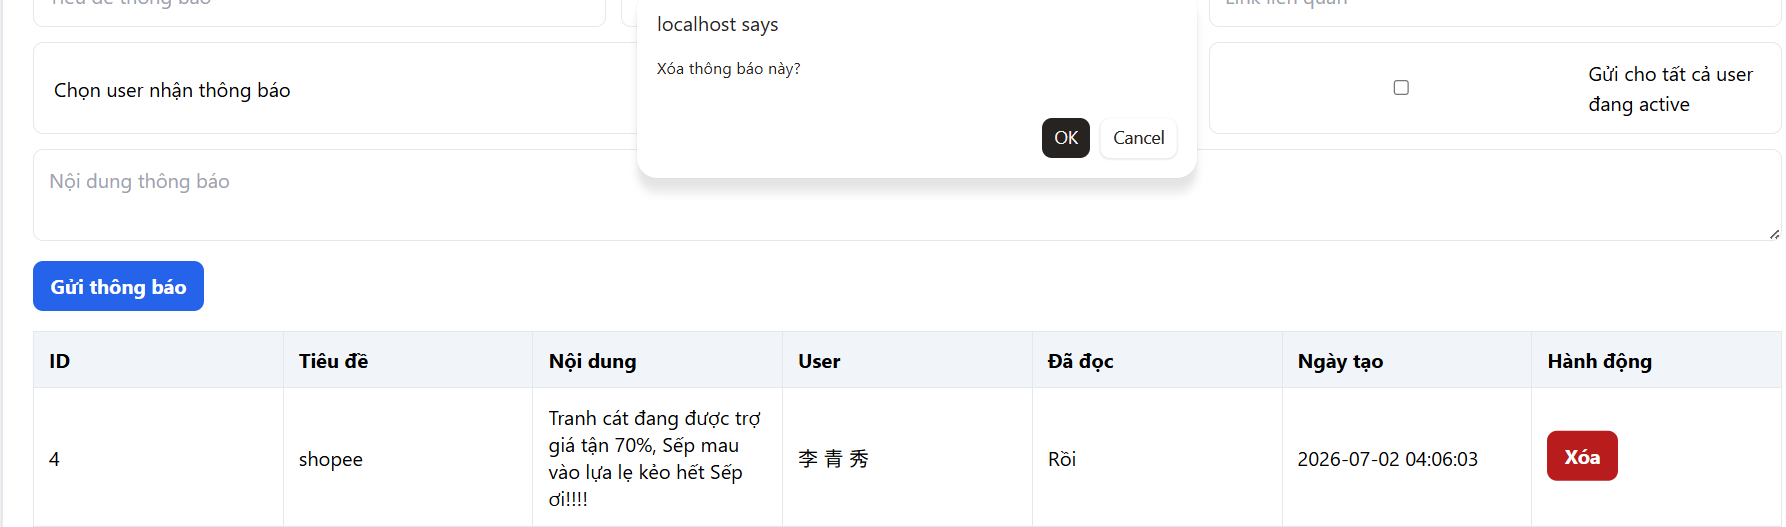
\includegraphics[width=\textwidth]{ad25.png}
    
    \label{fig:admin}
\end{figure}
\begin{itemize}[label=-]
    \item Users can view notifications on the notification page.
\end{itemize}
\begin{figure}[H]
	\centering
    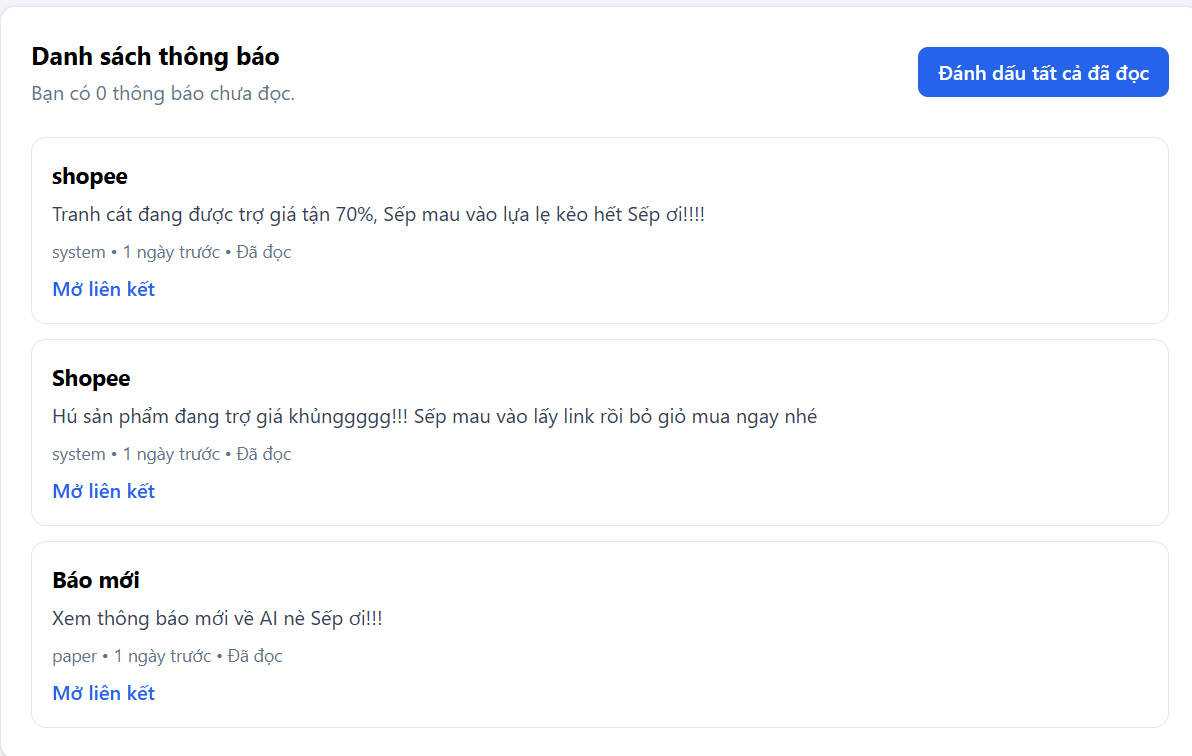
\includegraphics[width=\textwidth]{ad26.png}
   
    \label{fig:admin}
\end{figure}


\chapter{\centering\Large\bfseries IV. Software Design Description}
\addcontentsline{toc}{chapter}{ IV. Software Design Description}
\setcounter{section}{0}
\setcounter{subsection}{0}
\setcounter{subsubsection}{0}


\section{System Design}
\subsection{System Architecture}
\begin{figure}[H]
	\centering
	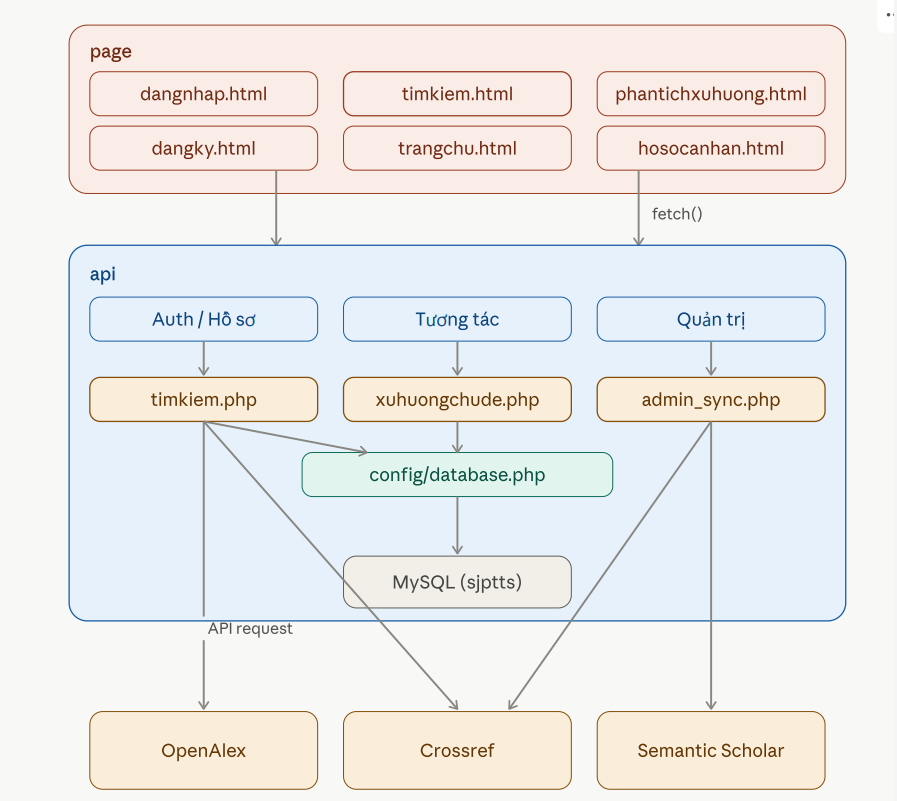
\includegraphics[width=0.8\textwidth]{ss.png}
	
	\label{fig:Overview_Diagram}
\end{figure}
\subsubsection{Frontend App}

The frontend application is developed using HTML, CSS, and JavaScript to provide the user interface for interacting with the system. It is responsible for presenting data, handling user interactions, and communicating with the backend system through HTTP requests.

\begin{itemize}
	\item \textbf{Pages}: Responsible for rendering the main user interfaces, including Login Page, Dashboard Page, Publication Search Page, Trend Analysis Page, Bookmark Page, and Notification Page.
	
	\item \textbf{Components}: Reusable user interface elements used to build application pages, such as search bars, filter panels, publication cards, charts, tables, and navigation menus.
	
	\item \textbf{Service}: Responsible for managing communication between the frontend and backend system through HTTP requests and responses, including sending requests and processing returned data.
\end{itemize}

\subsubsection{Backend System}

The backend system follows a layered architecture consisting of Controller Layer, Service Layer, and Repository Layer. This architecture improves maintainability, scalability, and separation of concerns.

\begin{itemize}
	\item \textbf{Controller Layer}: Handles incoming HTTP requests from the frontend, processes request validation, and forwards requests to the appropriate service layer.
	
	\item \textbf{Service Layer}: Contains business logic for processing publication data, trend analysis, user personalization, and system administration.
	
	\item \textbf{Repository Layer}: Responsible for interacting with the database, executing queries, and managing data persistence.
\end{itemize}

\subsubsection{External Systems}

The system integrates with external services to retrieve academic publication data and store system information.

\begin{itemize}
	\item \textbf{Academic APIs}: External academic data sources such as Semantic Scholar API, OpenAlex API, and Crossref API are used to retrieve publication metadata.
	
	\item \textbf{MySQL Database}: Stores user information, publication metadata, bookmarks, followed topics, notifications, and system configuration data.
\end{itemize}

\subsection{Package Diagram}
\subsubsection{Front End }
\begin{figure}[H]
	\centering
	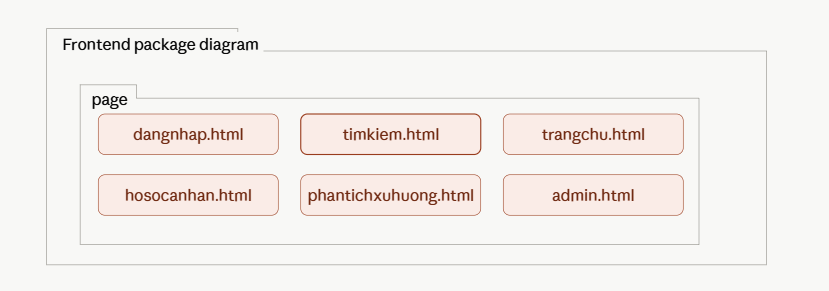
\includegraphics[width=\textwidth]{fe.png}
	\label{fig:backend_package_diagram}
\end{figure}


\newcolumntype{L}[1]{>{\raggedright\arraybackslash}p{#1}}

\begin{table}[h!]
	\centering

	\renewcommand{\arraystretch}{1.4}
	\small
	\rowcolors{2}{teal!6}{white}
	\begin{tabular}{|c|L{2.8cm}|L{8.5cm}|}
		\hline
		\rowcolor{teal!70}
		\textbf{\textcolor{white}{No}} & \textbf{\textcolor{white}{Page}} & \textbf{\textcolor{white}{Description}} \\
		\hline
		1 & \texttt{dangnhap.html}, \texttt{dangky.html} & Login and registration pages, calling \texttt{dangnhap.php} / \texttt{dangky.php}. \\
		\hline
		2 & \texttt{trangchu.html} & Public landing page (before login) --- hero banner introducing ScholarTrend, a search box for papers/authors/keywords, and a list of trending topics. \\
		\hline
		3 & \texttt{trangchu1.html} & Home page for logged-in users --- full navigation bar (Home, Trends, notifications, avatar), with links to profile, trend analysis, and notifications. \\
		\hline
		4 & \texttt{xemchitietbaibao.html} & Search page and article detail view --- calls \texttt{timkiem.php} to search, and \texttt{yeuthich.php} to save favorite papers. \\
		\hline
		5 & \texttt{phantichxuhuong.html} & Trend analysis page by topic --- calls \texttt{phantichxuhuong.php}, supports following topics and receiving notifications. \\
		\hline
		6 & \texttt{hosocanhan.html} & Account information page --- view/edit full name, email, username, email verification status; calls \texttt{hosocanhan.php}, \texttt{capnhathoso.php}, \texttt{dangxuat.php}. \\
		\hline
		7 & \texttt{yeuthich.html} & List of favorited papers, calls \texttt{yeuthich.php}. \\
		\hline
		8 & \texttt{xemthongbao.html} & Page displaying all notifications, calls \texttt{thongbao.php}. \\
		\hline
		9 & \texttt{admin.html} & System administration page --- manages users, topics, API sources, and data synchronization. \\
		\hline
	\end{tabular}
\end{table}
\subsubsection{Back End }
\begin{figure}[H]
	\centering
	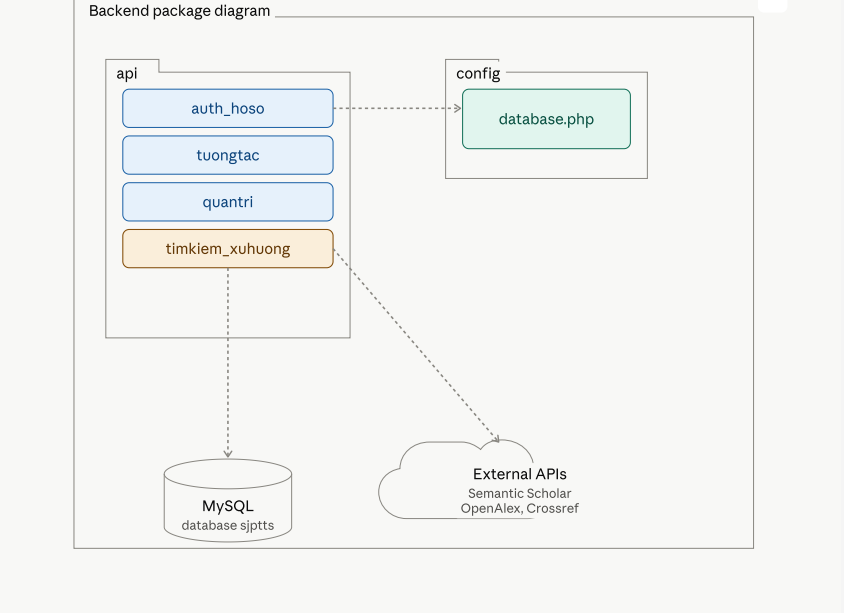
\includegraphics[width=\textwidth]{be.png}
	\label{fig:backend_package_diagram}
\end{figure}


\newcolumntype{L}[1]{>{\raggedright\arraybackslash}p{#1}}

\begin{table}[h!]
	\centering

	\renewcommand{\arraystretch}{1.4}
	\small % giảm cỡ chữ để không bị tràn trang
	\rowcolors{2}{teal!6}{white}
	\begin{tabular}{|c|L{3cm}|L{7.8cm}|}
		\hline
		\rowcolor{teal!70}
		\textbf{\textcolor{white}{No}} & \textbf{\textcolor{white}{Group / File}} & \textbf{\textcolor{white}{Description}} \\
		\hline
		1 & \texttt{dangnhap.php}, \texttt{dangky.php}, \texttt{dangxuat.php}, \texttt{check\_session.php} & Handles user authentication via PHP sessions, with hashed passwords (\texttt{password\_verify}). \\
		\hline
		2 & \texttt{hosocanhan.php}, \texttt{capnhathoso.php} & Retrieves and updates personal profile information. \\
		\hline
		3 & \texttt{timkiem.php} & Searches for research papers --- queries both OpenAlex and Crossref, then merges the results. \\
		\hline
		4 & \texttt{xuhuongchude.php} & Analyzes trending topics --- uses Crossref as the primary data source. \\
		\hline
		5 & \texttt{phantichxuhuong.php} & Processes trend analysis logic for topics already stored in the database. \\
		\hline
		6 & \texttt{theodoichude.php}, \texttt{yeuthich.php}, \texttt{thongbao.php} & Handles topic following, favorite papers, and user notifications. \\
		\hline
		7 & \texttt{admin\_users.php}, \texttt{admin\_papers.php}, \texttt{admin\_topics.php}, \texttt{admin\_api\_sources.php}, \texttt{admin\_notifications.php}, \texttt{admin\_check.php} & Administrative functions: managing users, papers, topics, API sources, and notifications. \\
		\hline
		8 & \texttt{admin\_sync.php} & Synchronizes paper data from OpenAlex and Semantic Scholar into the database. \\
		\hline
		9 & \texttt{api\_proxy.php} & Proxy that calls OpenAlex directly for the dashboard, with file-based caching (10-minute TTL) and rate limiting (5 requests/second). \\
		\hline
		10 & \texttt{config/database.php} & Establishes a PDO connection to the MySQL database (\texttt{sjptts}), required by most files in \texttt{api} via \texttt{require\_once}. \\
		\hline
	\end{tabular}
\end{table}

\clearpage
\section{Database Design}

\begin{figure}[h!]
\centering
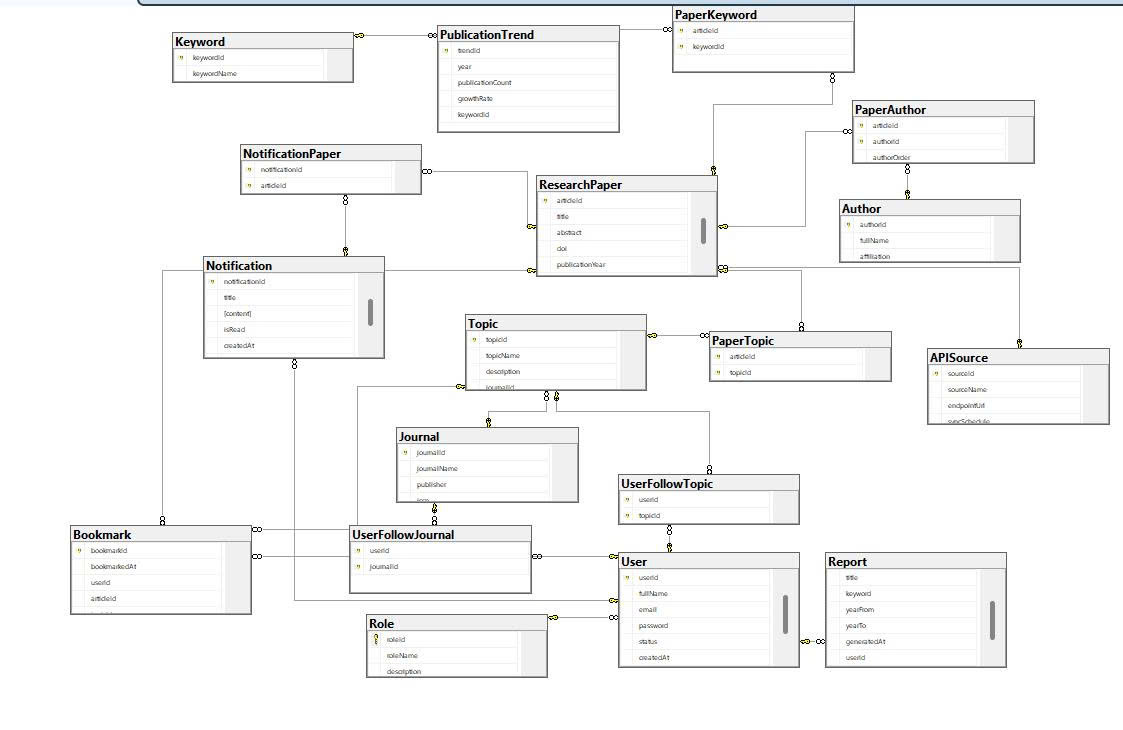
\includegraphics[width=\textwidth,
height=0.9\textheight,
keepaspectratio]{database.png}

\label{fig:erd}
\end{figure}

\clearpage
\noindent\textbf{Entities Description}
\subsection{Role Table}
\begin{longtable}{|p{3cm}|p{3cm}|p{6cm}|p{1.5cm}|p{1.5cm}|}
	\hline
	Field & Type & Description & PK & FK \\
	\hline
	roleId & INT & Role ID & Yes & No \\
	roleName & NVARCHAR(100) & Role name & No & No \\
	description & NVARCHAR(255) & Description & No & No \\
	\hline
\end{longtable}

% ================= USER =================
\subsection{User Table}
\begin{longtable}{|p{3cm}|p{3cm}|p{6cm}|p{1.5cm}|p{1.5cm}|}
	\hline
	Field & Type & Description & PK & FK \\
	\hline
	userId & INT & User ID & Yes & No \\
	fullName & NVARCHAR(150) & Full name & No & No \\
	email & NVARCHAR(150) & Email & No & No \\
	password & NVARCHAR(255) & Password & No & No \\
	status & NVARCHAR(50) & Status & No & No \\
	createdAt & DATETIME2 & Created time & No & No \\
	roleId & INT & Role reference & No & Yes → Role \\
	\hline
\end{longtable}

% ================= JOURNAL =================
\subsection{Journal Table}
\begin{longtable}{|p{3cm}|p{3cm}|p{6cm}|p{1.5cm}|p{1.5cm}|}
	\hline
	Field & Type & Description & PK & FK \\
	\hline
	journalId & INT & Journal ID & Yes & No \\
	journalName & NVARCHAR(200) & Journal name & No & No \\
	publisher & NVARCHAR(150) & Publisher & No & No \\
	issn & NVARCHAR(20) & ISSN & No & No \\
	\hline
\end{longtable}

% ================= USER FOLLOW JOURNAL =================
\subsection{UserFollowJournal (M:N)}
\begin{longtable}{|p{3cm}|p{3cm}|p{6cm}|p{1.5cm}|p{1.5cm}|}
	\hline
	Field & Type & Description & PK & FK \\
	\hline
	userId & INT & User & Yes (Composite) & Yes → User \\
	journalId & INT & Journal & Yes (Composite) & Yes → Journal \\
	\hline
\end{longtable}

% ================= TOPIC =================
\subsection{Topic Table}
\begin{longtable}{|p{3cm}|p{3cm}|p{6cm}|p{1.5cm}|p{1.5cm}|}
	\hline
	Field & Type & Description & PK & FK \\
	\hline
	topicId & INT & Topic ID & Yes & No \\
	topicName & NVARCHAR(150) & Topic name & No & No \\
	description & NVARCHAR(MAX) & Description & No & No \\
	journalId & INT & Journal reference & No & Yes → Journal \\
	\hline
\end{longtable}

% ================= USER FOLLOW TOPIC =================
\subsection{UserFollowTopic (M:N)}
\begin{longtable}{|p{3cm}|p{3cm}|p{6cm}|p{1.5cm}|p{1.5cm}|}
	\hline
	Field & Type & Description & PK & FK \\
	\hline
	userId & INT & User & Yes (Composite) & Yes → User \\
	topicId & INT & Topic & Yes (Composite) & Yes → Topic \\
	\hline
\end{longtable}

% ================= APISOURCE =================
\subsection{APISource Table}
\begin{longtable}{|p{3cm}|p{3cm}|p{6cm}|p{1.5cm}|p{1.5cm}|}
	\hline
	Field & Type & Description & PK & FK \\
	\hline
	sourceId & INT & Source ID & Yes & No \\
	sourceName & NVARCHAR(150) & Source name & No & No \\
	endpointUrl & NVARCHAR(500) & API URL & No & No \\
	syncSchedule & NVARCHAR(100) & Sync schedule & No & No \\
	\hline
\end{longtable}

% ================= AUTHOR =================
\subsection{Author Table}
\begin{longtable}{|p{3cm}|p{3cm}|p{6cm}|p{1.5cm}|p{1.5cm}|}
	\hline
	Field & Type & Description & PK & FK \\
	\hline
	authorId & INT & Author ID & Yes & No \\
	fullName & NVARCHAR(150) & Full name & No & No \\
	affiliation & NVARCHAR(255) & Affiliation & No & No \\
	\hline
\end{longtable}

% ================= KEYWORD =================
\subsection{Keyword Table}
\begin{longtable}{|p{3cm}|p{3cm}|p{6cm}|p{1.5cm}|p{1.5cm}|}
	\hline
	Field & Type & Description & PK & FK \\
	\hline
	keywordId & INT & Keyword ID & Yes & No \\
	keywordName & NVARCHAR(100) & Keyword & No & No \\
	\hline
\end{longtable}

% ================= RESEARCH PAPER =================
\subsection{Research Paper Table}
\begin{longtable}{|p{3cm}|p{3cm}|p{6cm}|p{1.5cm}|p{1.5cm}|}
	\hline
	Field & Type & Description & PK & FK \\
	\hline
	articleId & INT & Paper ID & Yes & No \\
	title & NVARCHAR(500) & Title & No & No \\
	abstract & NVARCHAR(MAX) & Abstract & No & No \\
	doi & NVARCHAR(200) & DOI & No & No \\
	publicationYear & INT & Year & No & No \\
	sourceId & INT & API Source & No & Yes → APISource \\
	\hline
\end{longtable}

% ================= PAPER TOPIC =================
\subsection{PaperTopic (M:N)}
\begin{longtable}{|p{3cm}|p{3cm}|p{6cm}|p{1.5cm}|p{1.5cm}|}
	\hline
	Field & Type & Description & PK & FK \\
	\hline
	articleId & INT & Paper & Yes (Composite) & Yes → ResearchPaper \\
	topicId & INT & Topic & Yes (Composite) & Yes → Topic \\
	\hline
\end{longtable}

% ================= PAPER KEYWORD =================
\subsection{PaperKeyword (M:N)}
\begin{longtable}{|p{3cm}|p{3cm}|p{6cm}|p{1.5cm}|p{1.5cm}|}
	\hline
	Field & Type & Description & PK & FK \\
	\hline
	articleId & INT & Paper & Yes (Composite) & Yes → ResearchPaper \\
	keywordId & INT & Keyword & Yes (Composite) & Yes → Keyword \\
	\hline
\end{longtable}

% ================= PAPER AUTHOR =================
\subsection{PaperAuthor (M:N)}
\begin{longtable}{|p{3cm}|p{3cm}|p{6cm}|p{1.5cm}|p{1.5cm}|}
	\hline
	Field & Type & Description & PK & FK \\
	\hline
	articleId & INT & Paper & Yes (Composite) & Yes → ResearchPaper \\
	authorId & INT & Author & Yes (Composite) & Yes → Author \\
	authorOrder & INT & Author order & No & No \\
	\hline
\end{longtable}

% ================= PUBLICATION TREND =================
\subsection{PublicationTrend Table}
\begin{longtable}{|p{3cm}|p{3cm}|p{6cm}|p{1.5cm}|p{1.5cm}|}
	\hline
	Field & Type & Description & PK & FK \\
	\hline
	trendId & INT & Trend ID & Yes & No \\
	year & INT & Year & No & No \\
	publicationCount & INT & Count & No & No \\
	growthRate & FLOAT & Growth rate & No & No \\
	keywordId & INT & Keyword & No & Yes → Keyword \\
	\hline
\end{longtable}

% ================= REPORT =================
\subsection{Report Table}
\begin{longtable}{|p{3cm}|p{3cm}|p{6cm}|p{1.5cm}|p{1.5cm}|}
	\hline
	Field & Type & Description & PK & FK \\
	\hline
	reportId & INT & Report ID & Yes & No \\
	title & NVARCHAR(300) & Title & No & No \\
	keyword & NVARCHAR(200) & Keyword & No & No \\
	yearFrom & INT & From year & No & No \\
	yearTo & INT & To year & No & No \\
	generatedAt & DATETIME2 & Created time & No & No \\
	userId & INT & User & No & Yes → User \\
	\hline
\end{longtable}

% ================= NOTIFICATION =================
\subsection{Notification Table}
\begin{longtable}{|p{3cm}|p{3cm}|p{6cm}|p{1.5cm}|p{1.5cm}|}
	\hline
	Field & Type & Description & PK & FK \\
	\hline
	notificationId & INT & Notification ID & Yes & No \\
	title & NVARCHAR(300) & Title & No & No \\
	content & NVARCHAR(MAX) & Content & No & No \\
	isRead & BIT & Read status & No & No \\
	createdAt & DATETIME2 & Created time & No & No \\
	userId & INT & User & No & Yes → User \\
	\hline
\end{longtable}

% ================= NOTIFICATION PAPER =================
\subsection{NotificationPaper (M:N)}
\begin{longtable}{|p{3cm}|p{3cm}|p{6cm}|p{1.5cm}|p{1.5cm}|}
	\hline
	Field & Type & Description & PK & FK \\
	\hline
	notificationId & INT & Notification & Yes (Composite) & Yes → Notification \\
	articleId & INT & Paper & Yes (Composite) & Yes → ResearchPaper \\
	\hline
\end{longtable}

% ================= BOOKMARK =================
\subsection{Bookmark Table}
\begin{longtable}{|p{3cm}|p{3cm}|p{6cm}|p{1.5cm}|p{1.5cm}|}
	\hline
	Field & Type & Description & PK & FK \\
	\hline
	bookmarkId & INT & Bookmark ID & Yes & No \\
	bookmarkedAt & DATETIME2 & Time saved & No & No \\
	userId & INT & User & No & Yes → User \\
	articleId & INT & Paper & No & Yes → ResearchPaper \\
	topicId & INT & Topic & No & Yes → Topic \\
	\hline
\end{longtable}
\section{ Detail Design}
\subsection{Register}
\subsubsection{Class Diagram}
\begin{figure}[H]
	\centering
	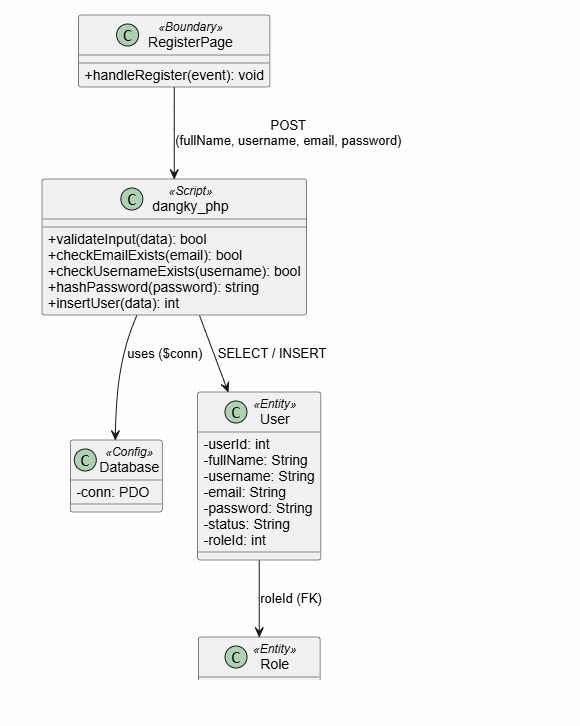
\includegraphics[width=\textwidth]{dk.png}

	\label{fig:class-track-publication-trends}
\end{figure}

\subsubsection{Sequence Diagram} 
\begin{figure}[H]
	\centering
	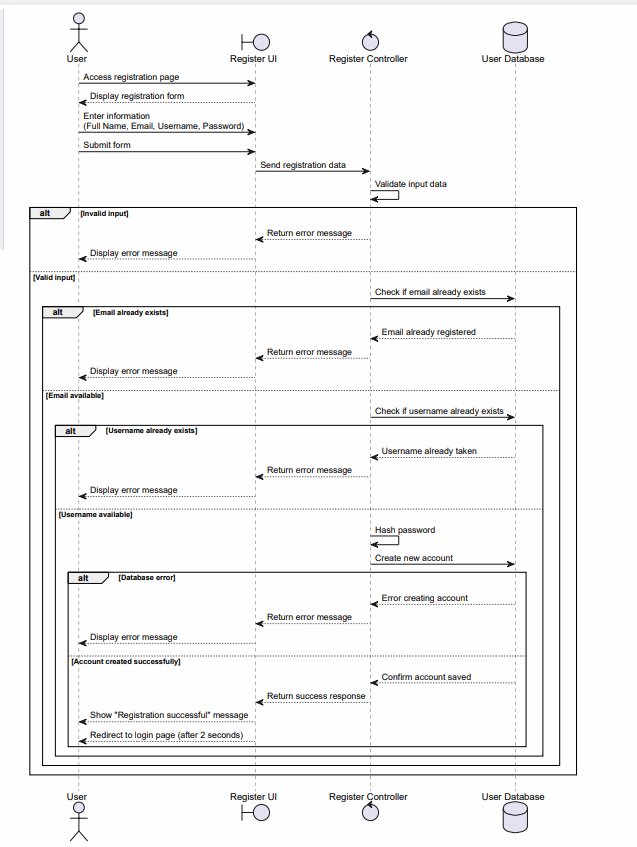
\includegraphics[width=\textwidth]{ttdk.png}

	\label{fig:erd}
\end{figure}



\subsection{Login}
\subsubsection{Class Diagram}
\begin{figure}[H]
	\centering
	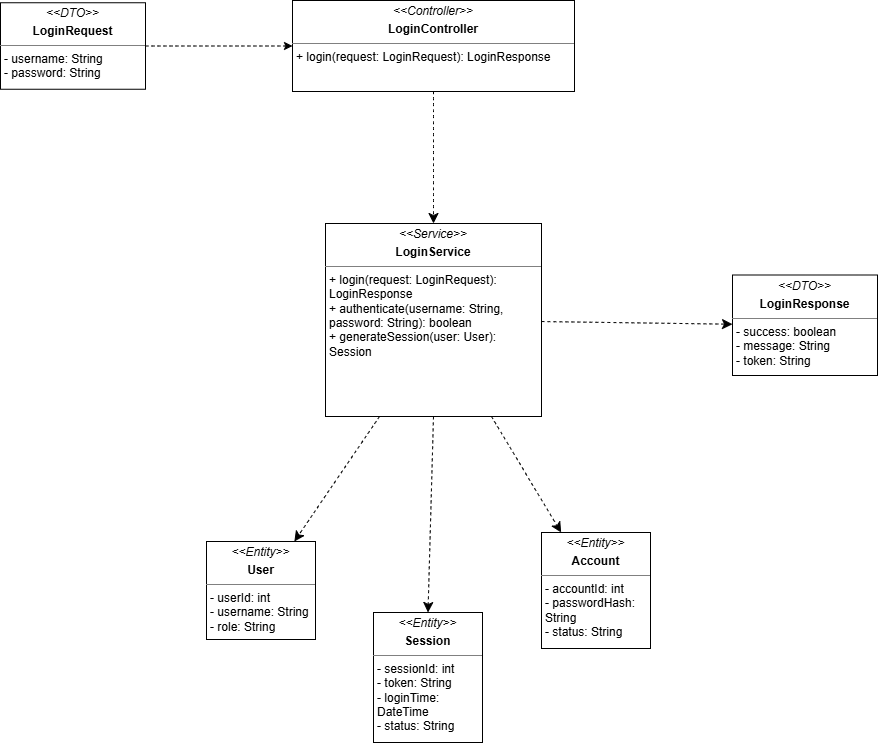
\includegraphics[width=\textwidth]{CDLogin.png}

	\label{fig:class-track-publication-trends}
\end{figure}
\subsubsection{Sequence Diagram}
\begin{figure}[H]
	\centering
	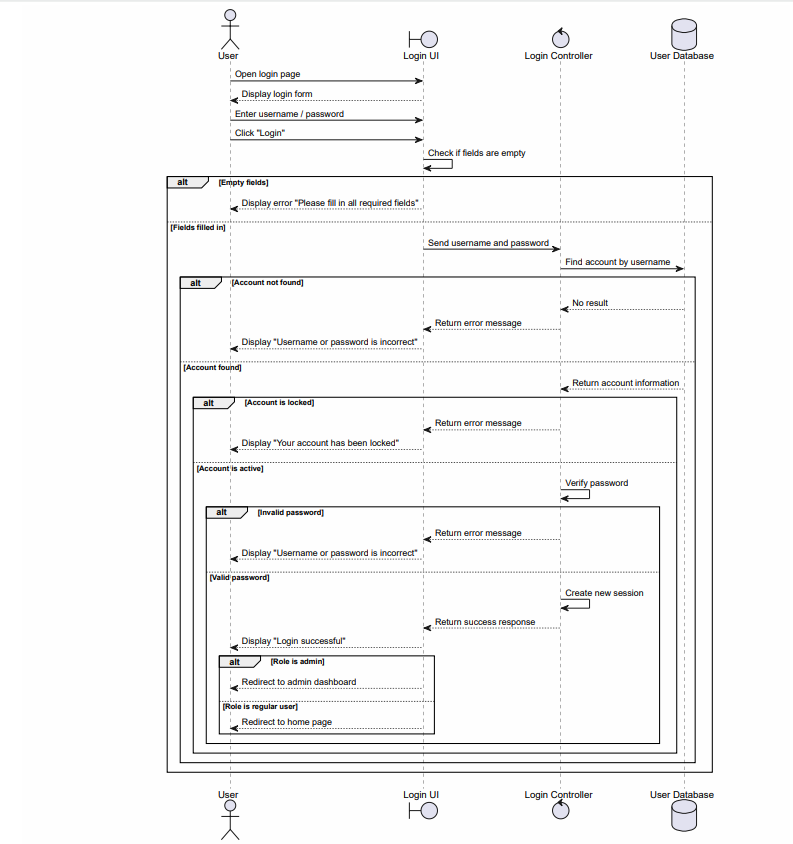
\includegraphics[width=\textwidth]{ttdn.png}

	\label{fig:erd}
\end{figure}



%-------------------------------------------------
\subsection{Search Research Papers}
\subsubsection{Class Diagram}
\begin{figure}[H]
	\centering
	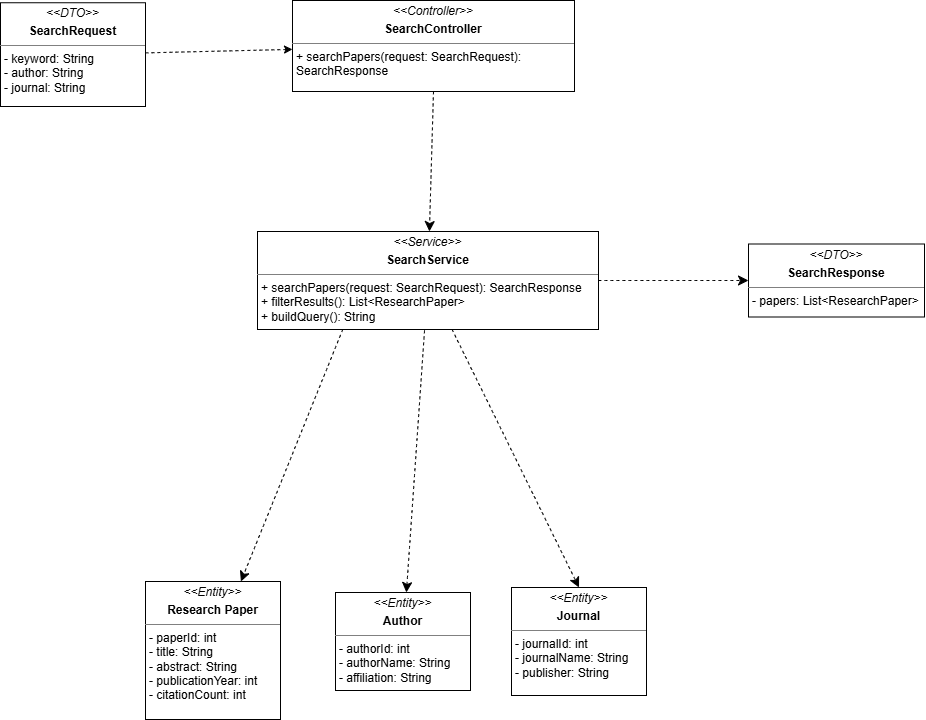
\includegraphics[width=\textwidth]{CDSearchResearchPaper.png}

	\label{fig:class-track-publication-trends}
\end{figure}

\subsubsection{Sequence Diagram}
\begin{figure}[H]
	\centering
	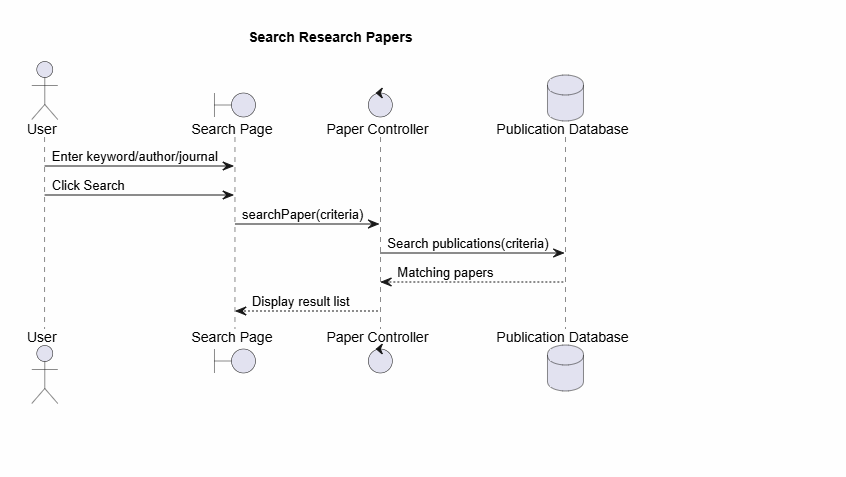
\includegraphics[width=\textwidth]{tk.png}

	\label{fig:erd}
\end{figure}



%-------------------------------------------------
\subsection{View Paper Details}
\subsubsection{Class Diagram}
\begin{figure}[H]
	\centering
	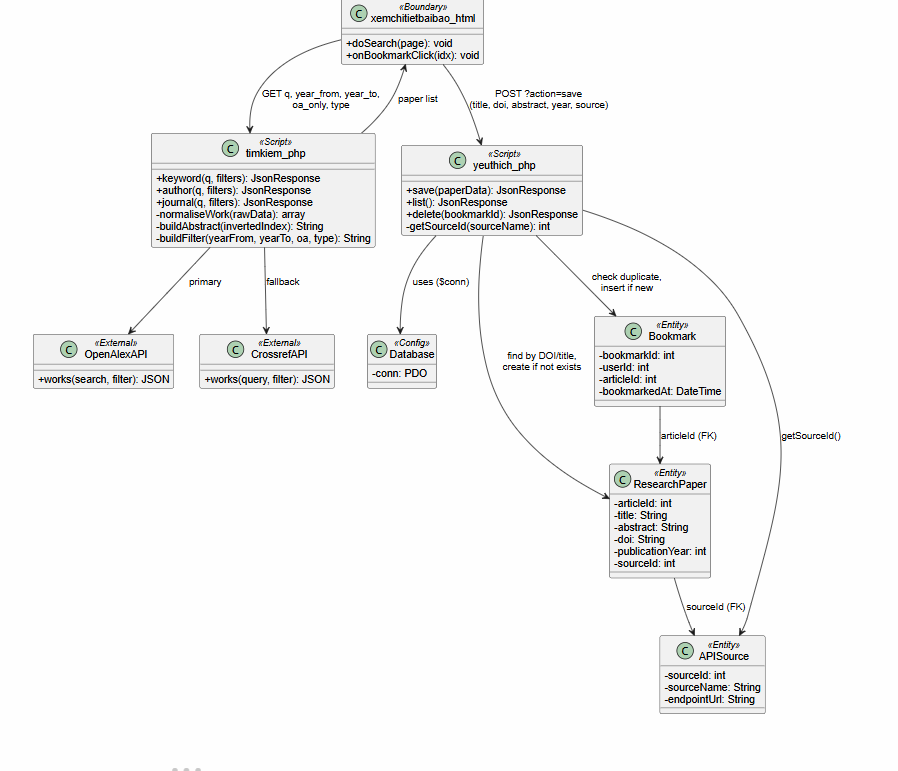
\includegraphics[width=0.6\textwidth]{chitiet.png}

	\label{fig:class-track-publication-trends}
\end{figure}

\subsubsection{Sequence Diagram}
\begin{figure}[H]
	\centering
	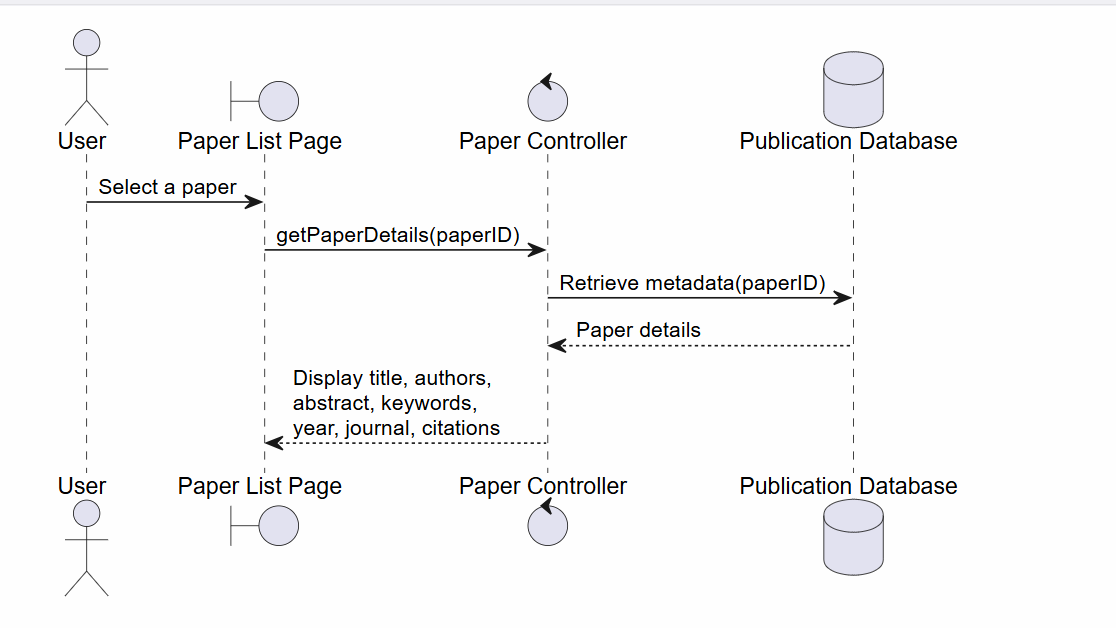
\includegraphics[width=\textwidth]{ct.png}

	\label{fig:sequence-view-paper-details}
\end{figure}



%-------------------------------------------------
\subsection{Save Bookmarks}
\subsubsection{Class Diagram}
\begin{figure}[H]
	\centering
	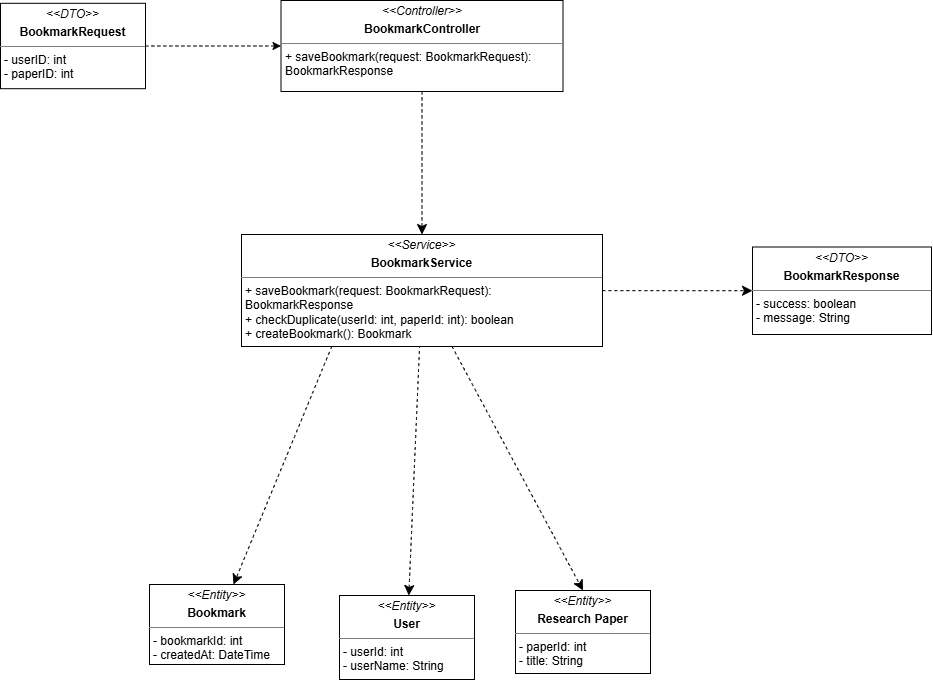
\includegraphics[width=0.6\textwidth]{CDBookmark.png}

	\label{fig:class-track-publication-trends}
\end{figure}
\subsubsection{Sequence Diagram}
\begin{figure}[H]
	\centering
	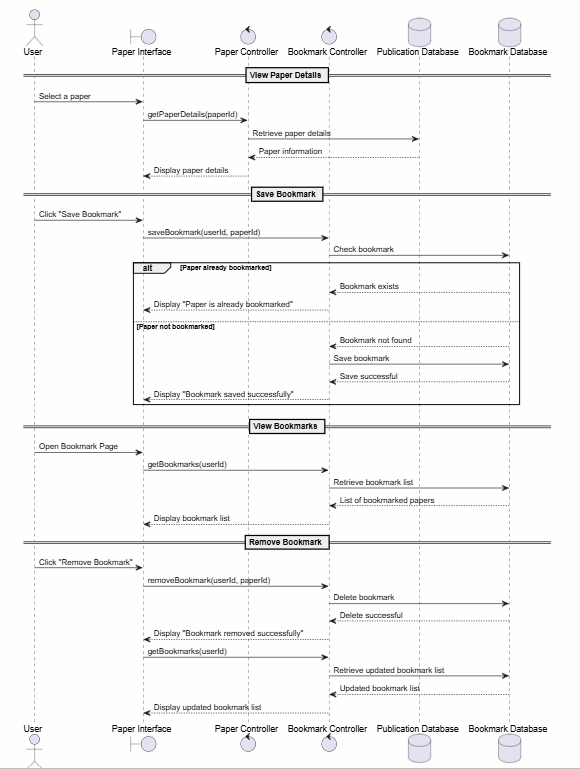
\includegraphics[width=\textwidth]{yttt.png}

	\label{fig:sequence-save-bookmarks}
\end{figure}



%-------------------------------------------------
\subsection{Track Publication Trends}
\subsubsection{Class Diagram}
\begin{figure}[H]
	\centering
	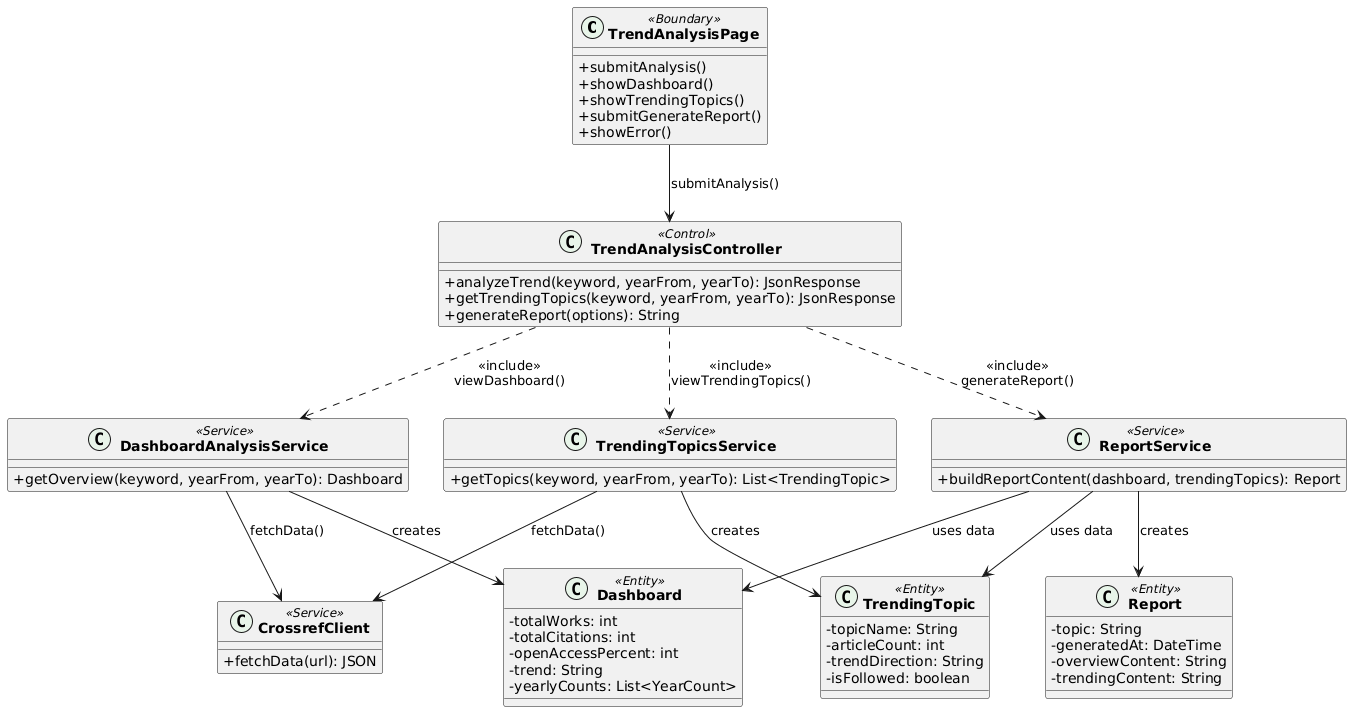
\includegraphics[width=\textwidth]{CDTrackPublicationTrends.png}

	\label{fig:class-track-publication-trends}
\end{figure}
%---------------
\subsubsection{Sequence Diagram}
\begin{figure}[H]
	\centering
	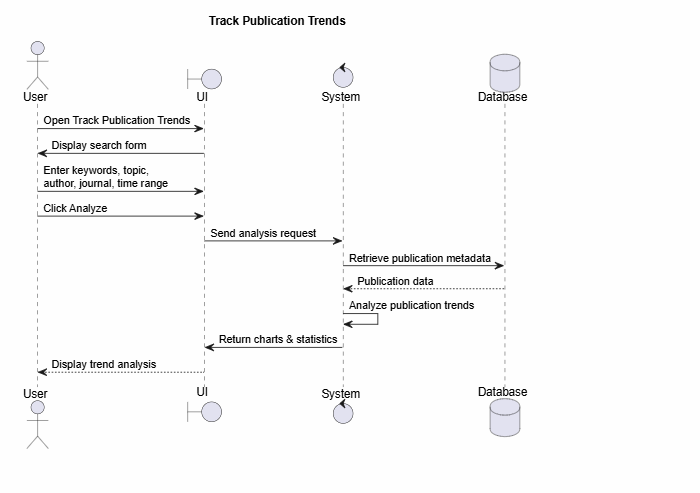
\includegraphics[width=\textwidth]{xh.png}

	\label{fig:sequence-track-publication-trends}
\end{figure}

----------------------------------
\subsection{View Dashboard}
\subsubsection{Class Diagram}
\begin{figure}[H]
	\centering
	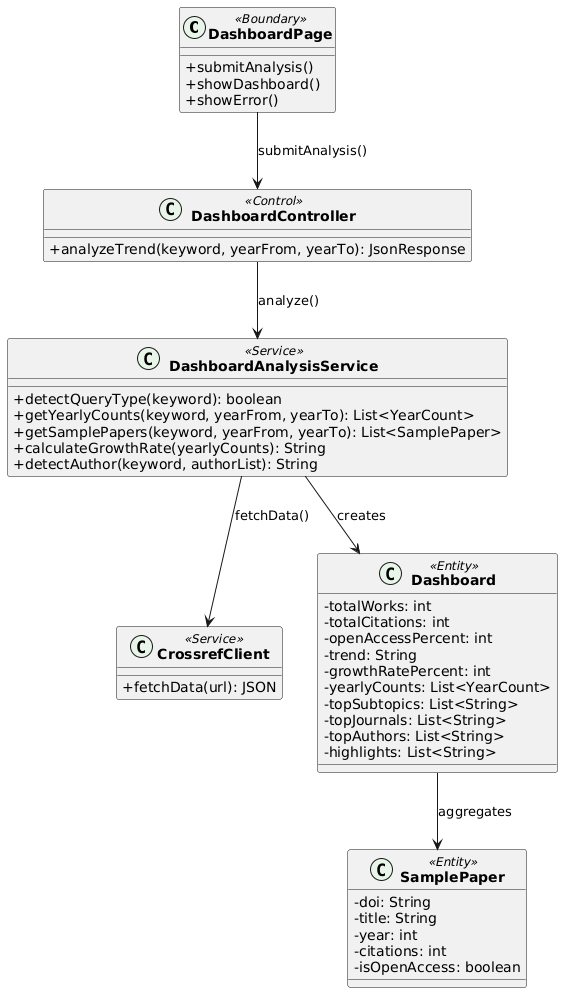
\includegraphics[width=0.6\textwidth]{CDViewDashboard.png}

	\label{fig:class-view-dashboard}
\end{figure}
\subsubsection{Sequence Diagram}
\begin{figure}[H]
	\centering
	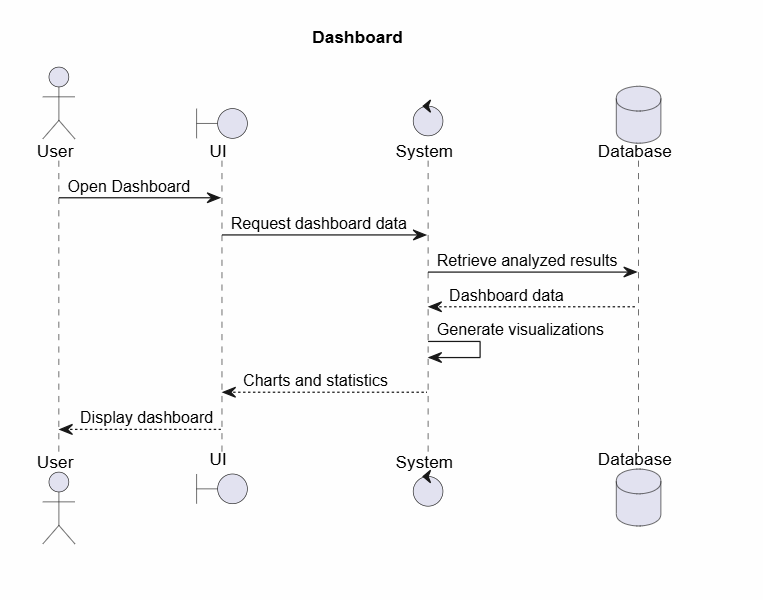
\includegraphics[width=\textwidth]{dkk.png}

	\label{fig:erd}
\end{figure}


%-------------------------------------------------
\subsection{Generate Reports}
\subsubsection{Class Diagram}
\begin{figure}[H]
	\centering
	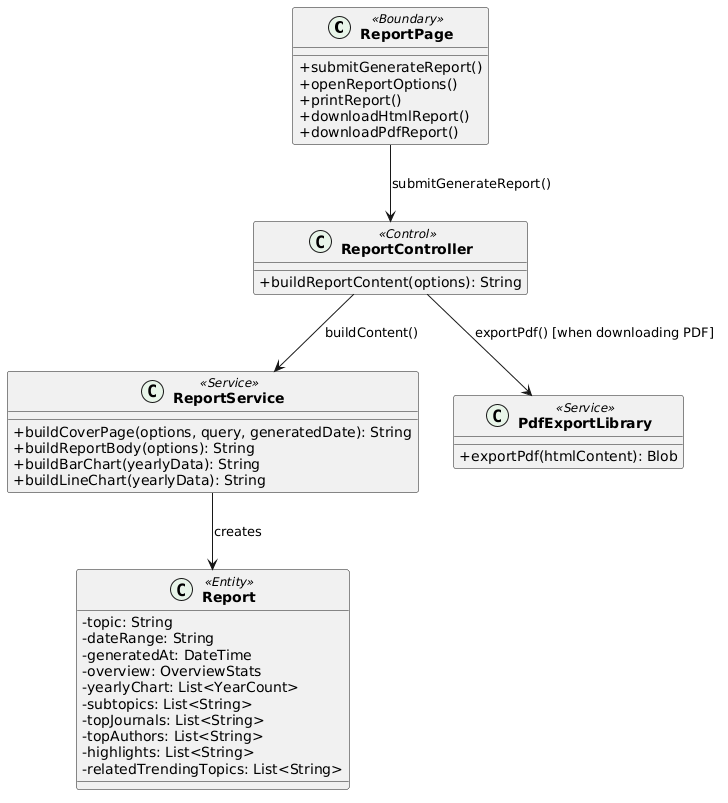
\includegraphics[width=\textwidth]{CDReportGenerate.png}
	
	\label{fig:class-generate-reports}
\end{figure}
\subsubsection{Sequence Diagram}
\begin{figure}[H]
	\centering
	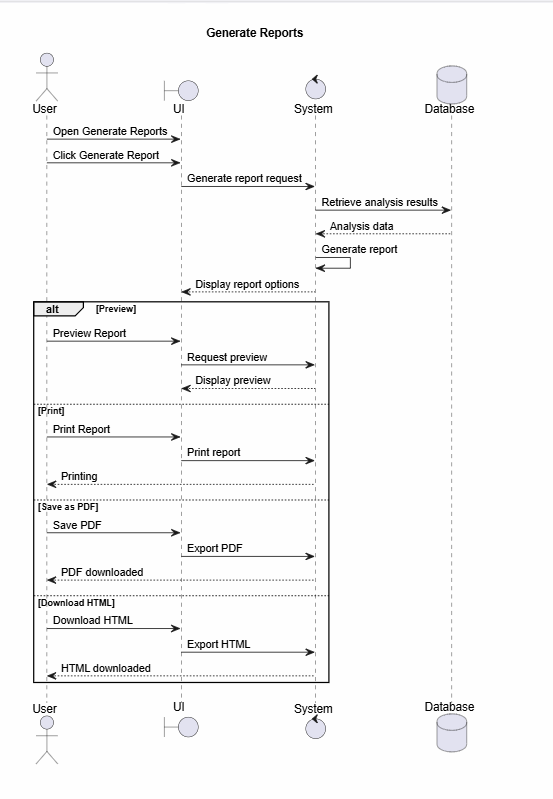
\includegraphics[height=0.9\textheight,keepaspectratio]{bc.png}

	\label{fig:sequence_generate_repoclearpagerts}
\end{figure}


%-------------------------------------------------
\subsection{View Trending Topics}
\subsubsection{Class Diagram}
\begin{figure}[H]
	\centering
	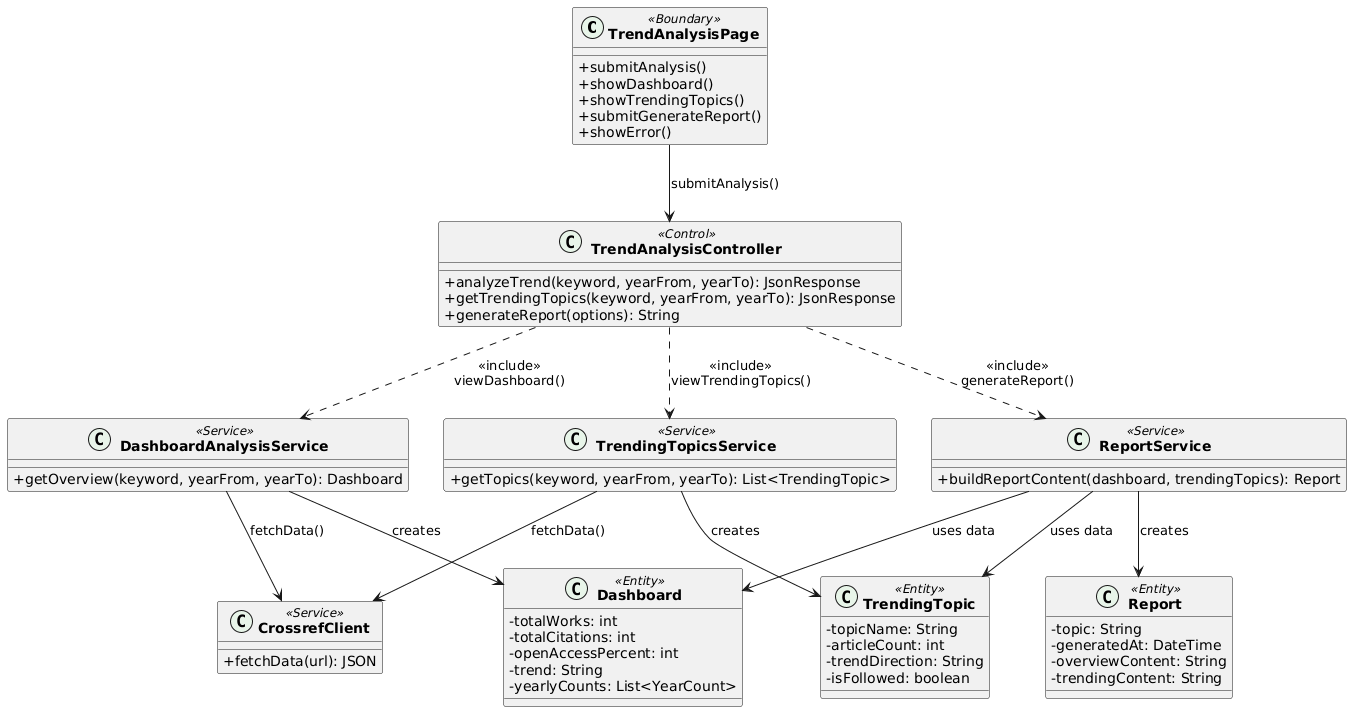
\includegraphics[width=\textwidth]{CDViewTrendingTopics.png}

	\label{fig:class-view-trending-topics}
\end{figure}

\subsubsection{Sequence Diagram}
\begin{figure}[H]
	\centering
	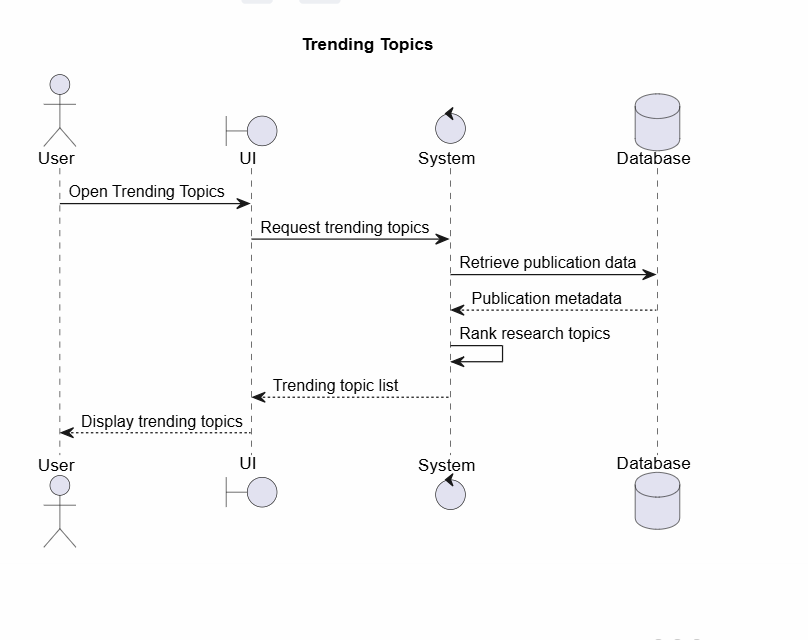
\includegraphics[width=\textwidth]{cdxh.png}

	\label{fig:erd}
\end{figure}


%-------------------------------------------------
\subsection{Follow Topics}
\subsubsection{Class Diagram}
\begin{figure}[H]
	\centering
	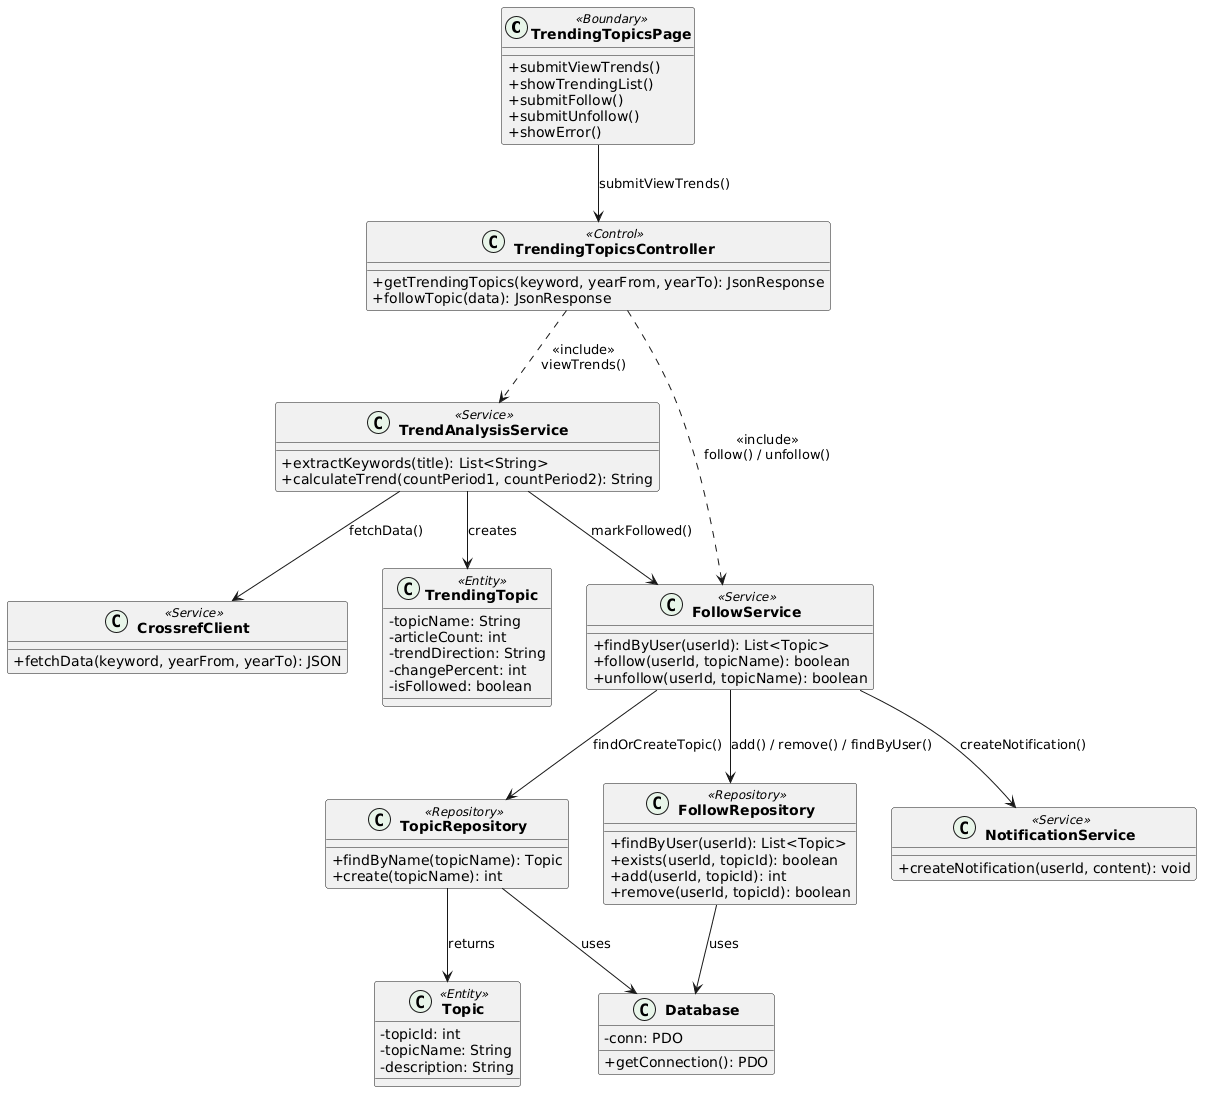
\includegraphics[width=\textwidth]{CDFollowTopics.png}

	\label{fig:class-follow-topics}
\end{figure}
\subsubsection{Sequence Diagram}
\begin{figure}[H]
	\centering
	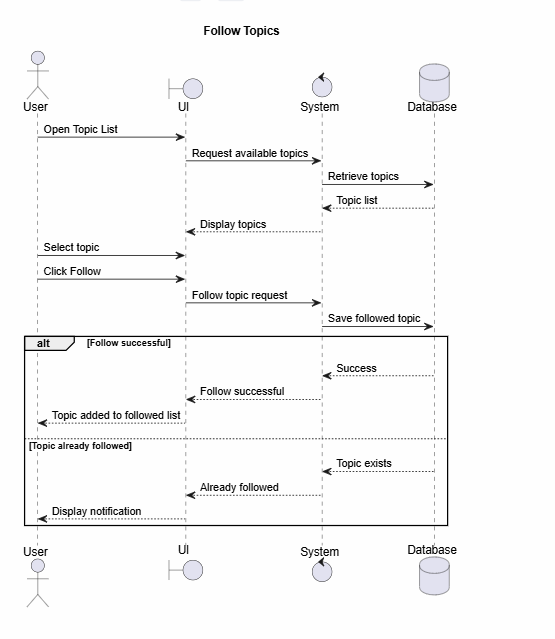
\includegraphics[width=\textwidth]{td.png}

	\label{fig:erd}
\end{figure}



%-------------------------------------------------
\subsection{Receive Notifications}

\subsubsection{Sequence Diagram}
\begin{figure}[H]
	\centering
	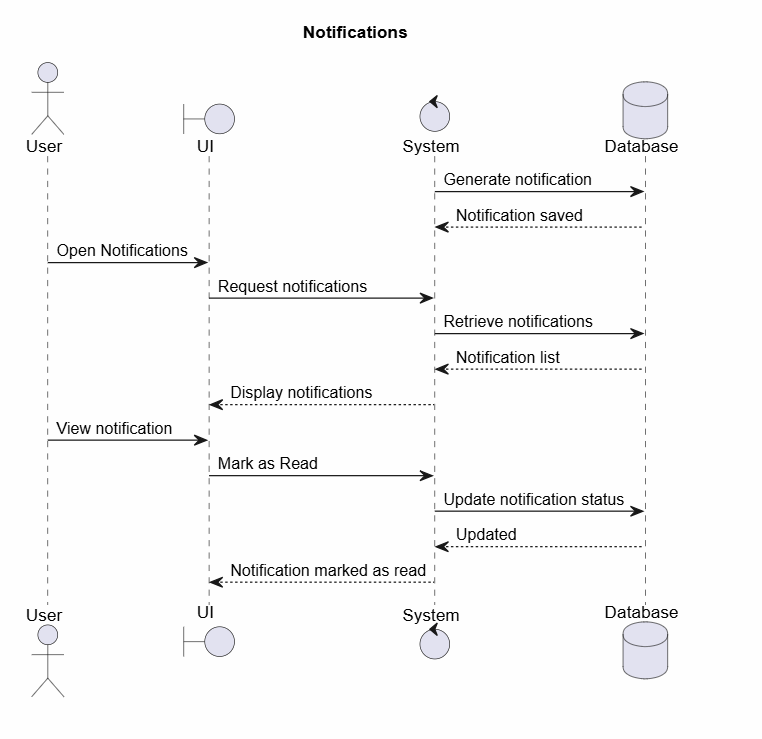
\includegraphics[width=\textwidth]{tb.png}

	\label{fig:erd}
\end{figure}


%-------------------------------------------------
\subsection{Manage System}
\subsubsection{Class Diagram}
\begin{figure}[H]
	\centering
	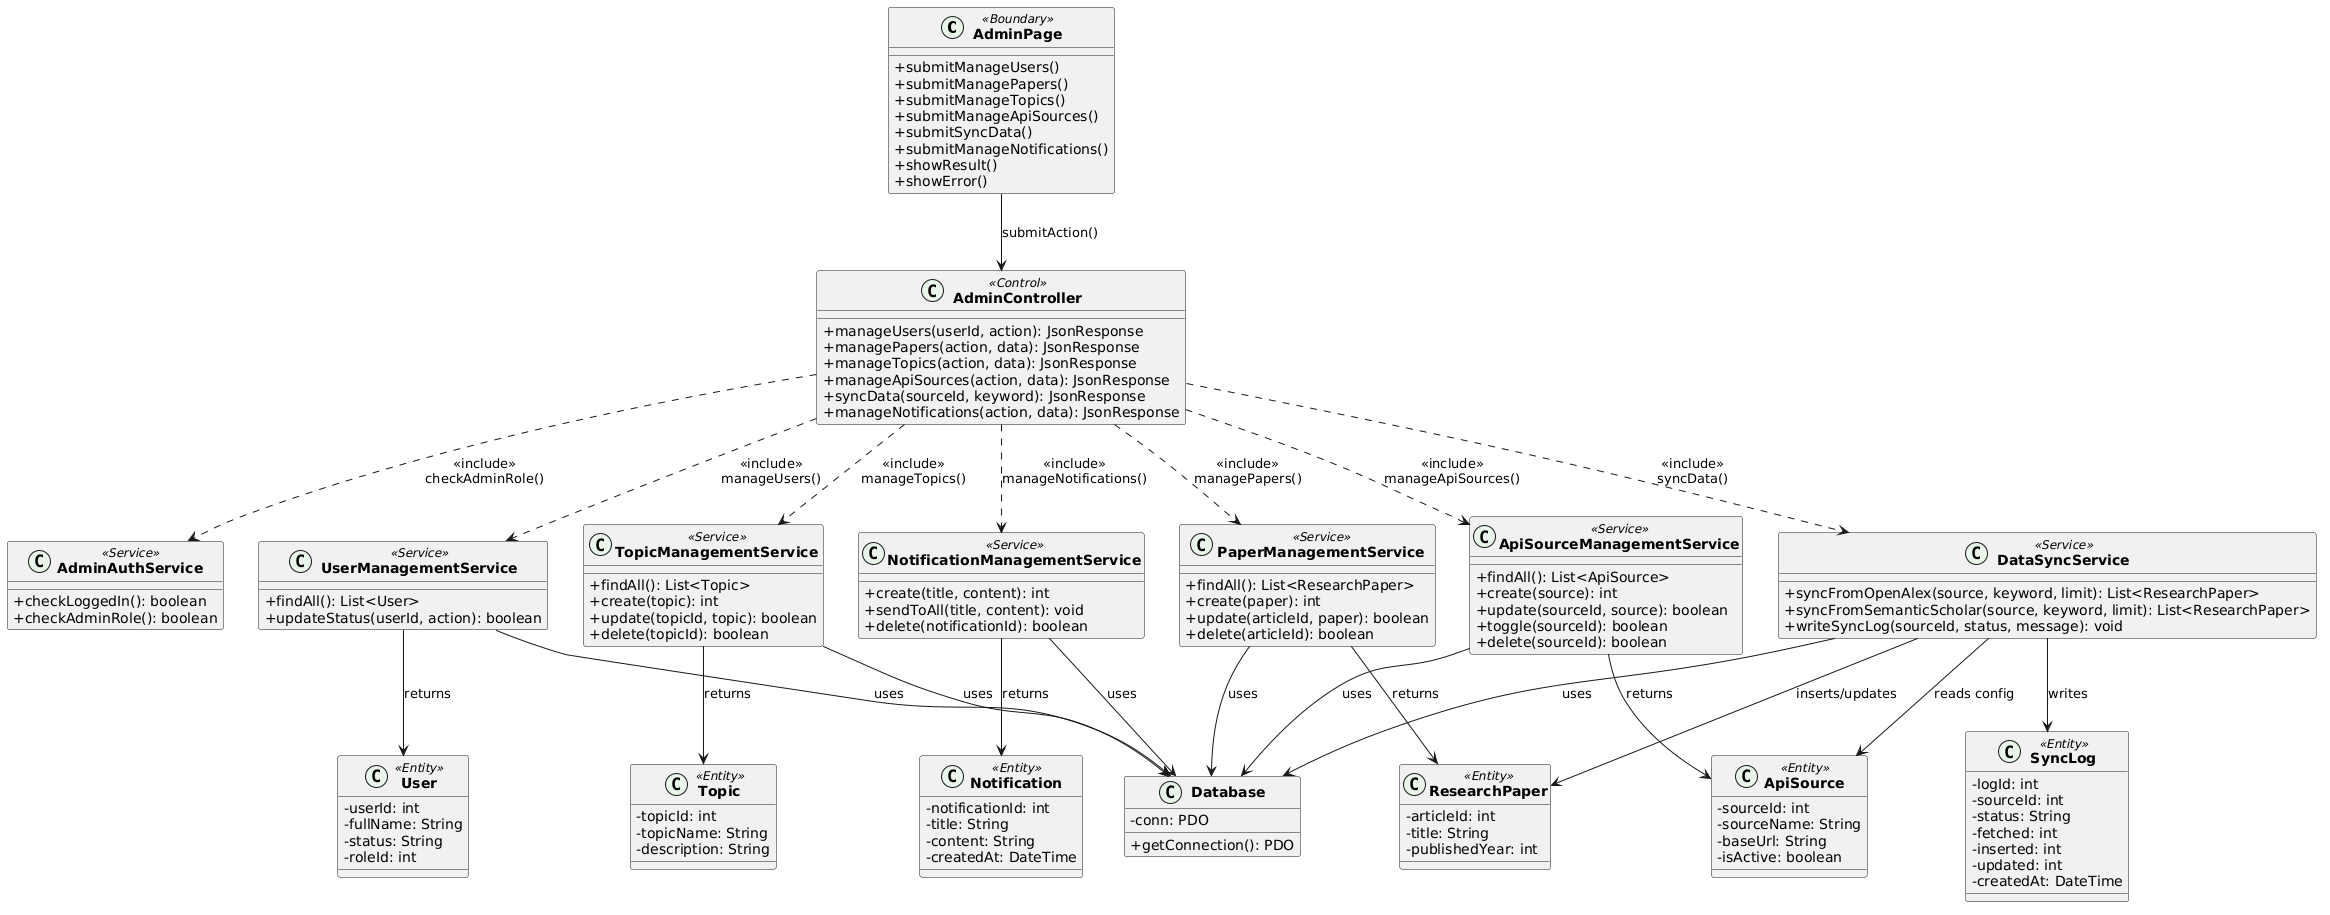
\includegraphics[width=0.9\textwidth]{CDManageSystem.png}

	\label{fig:erd}
\end{figure}
\subsubsection{Sequence Diagram}
\begin{figure}[H]
	\centering
	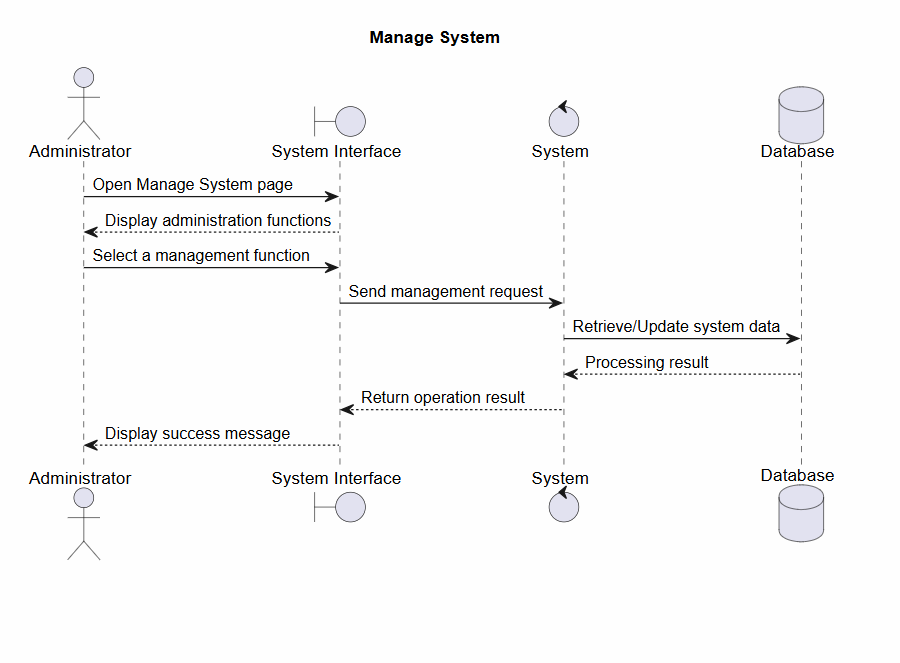
\includegraphics[width=0.9\textwidth]{ht.png}

	\label{fig:erd}
\end{figure}



%-------------------------------------------------
\subsection{Manage User}
\subsubsection{Class Diagram}
\begin{figure}[H]
	\centering
	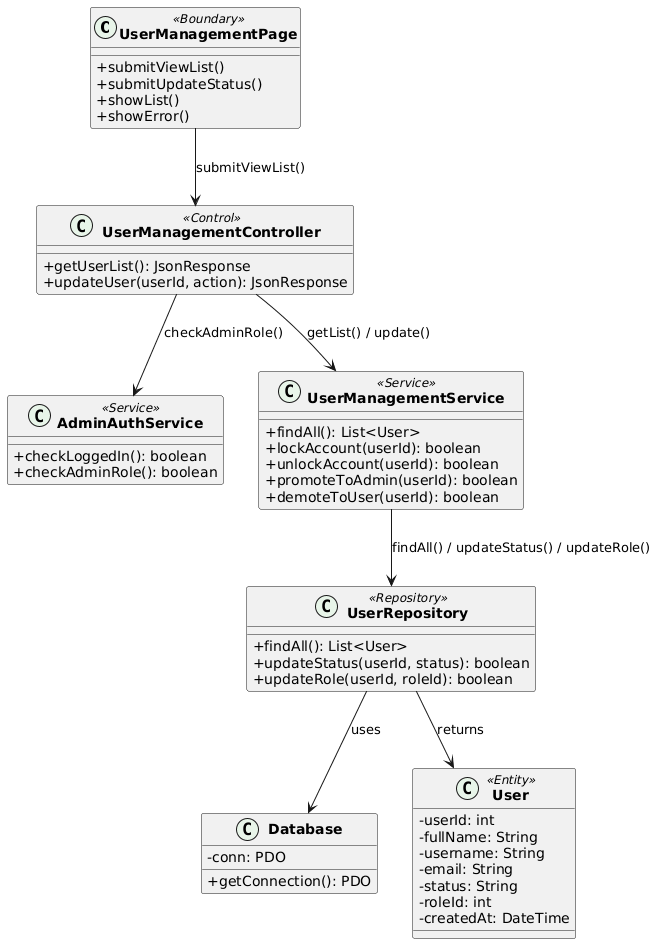
\includegraphics[width=0.8\textwidth]{CDManageUser.png}

	\label{fig:erd}
\end{figure}

\subsubsection{Sequence Diagram}
\begin{figure}[H]
	\centering
	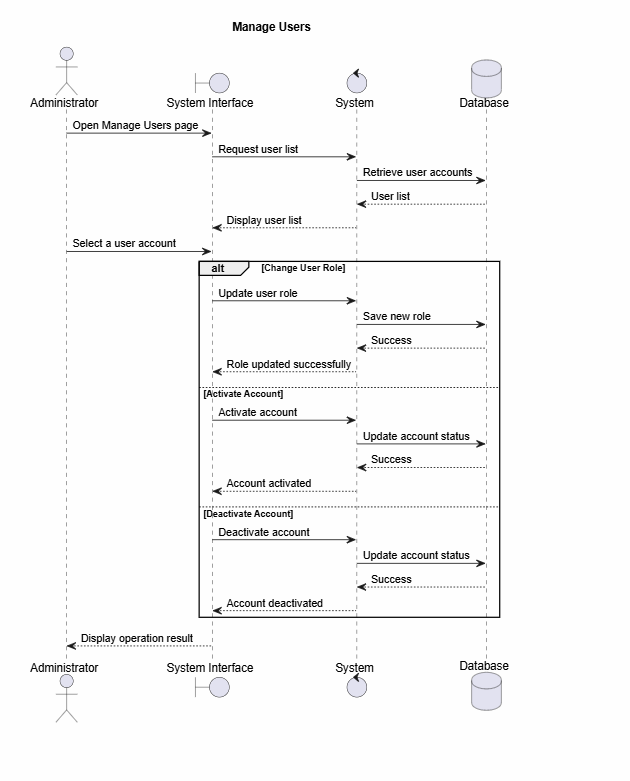
\includegraphics[width=0.7\textwidth]{nd.png}

	\label{fig:sequence_manage_users}
\end{figure}


%-------------------------------------------------
\subsection{Configure API Sources}
\subsubsection{Class Diagram}
\begin{figure}[H]
	\centering
	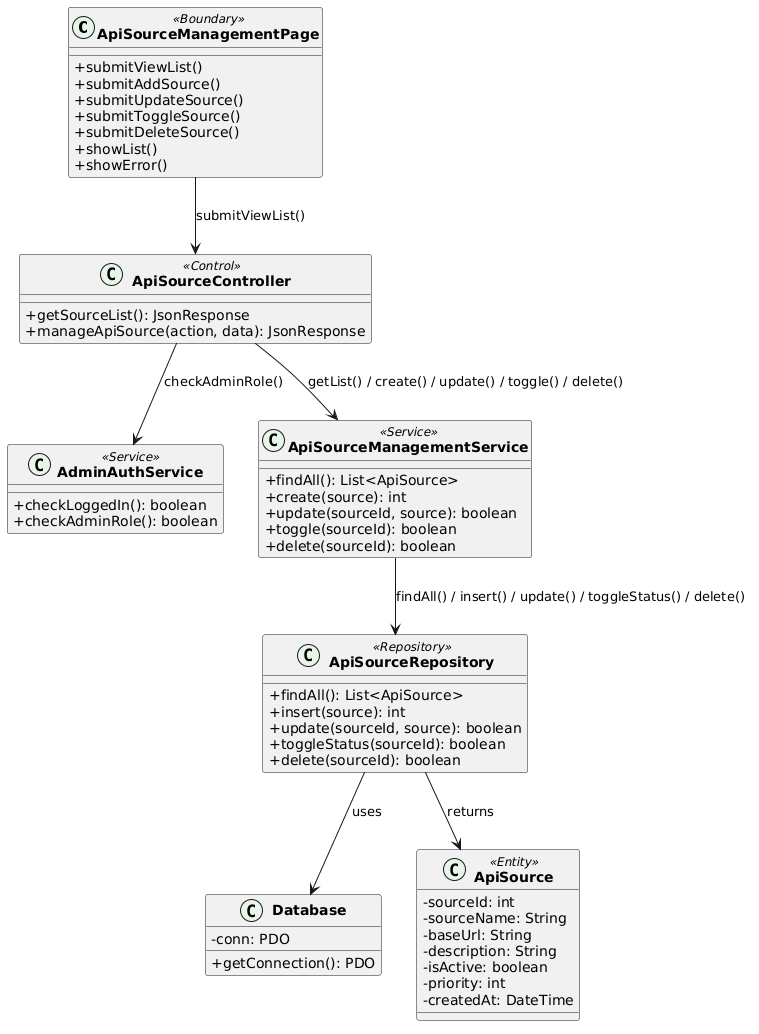
\includegraphics[width=0.8\textwidth]{CDManageAPI.png}

	\label{fig:erd}
\end{figure}
\subsubsection{Sequence Diagram}
\begin{figure}[H]
	\centering
	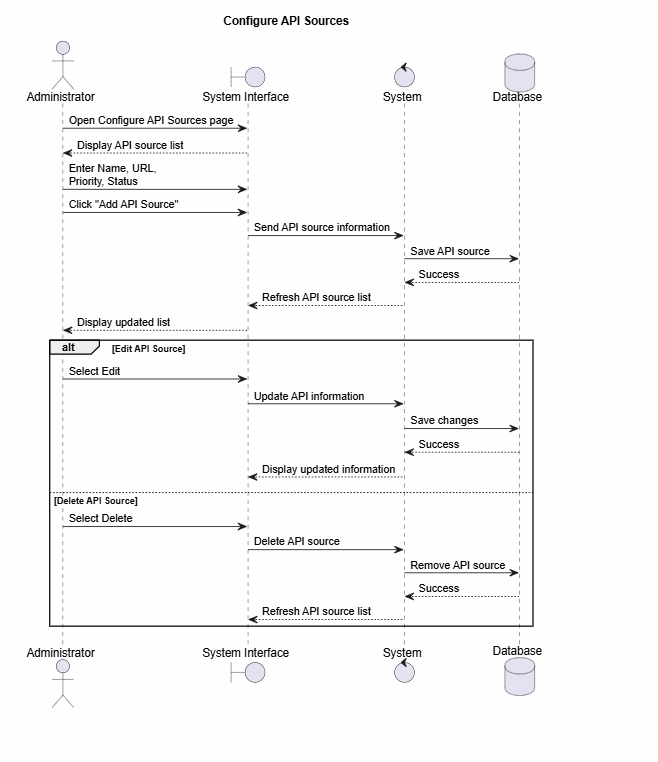
\includegraphics[width=\textwidth]{apii.png}

	\label{fig:erd}
\end{figure}



%-------------------------------------------------
\subsection{Sync Academic Data}
\subsubsection{Class Diagram}
\begin{figure}[H]
	\centering
	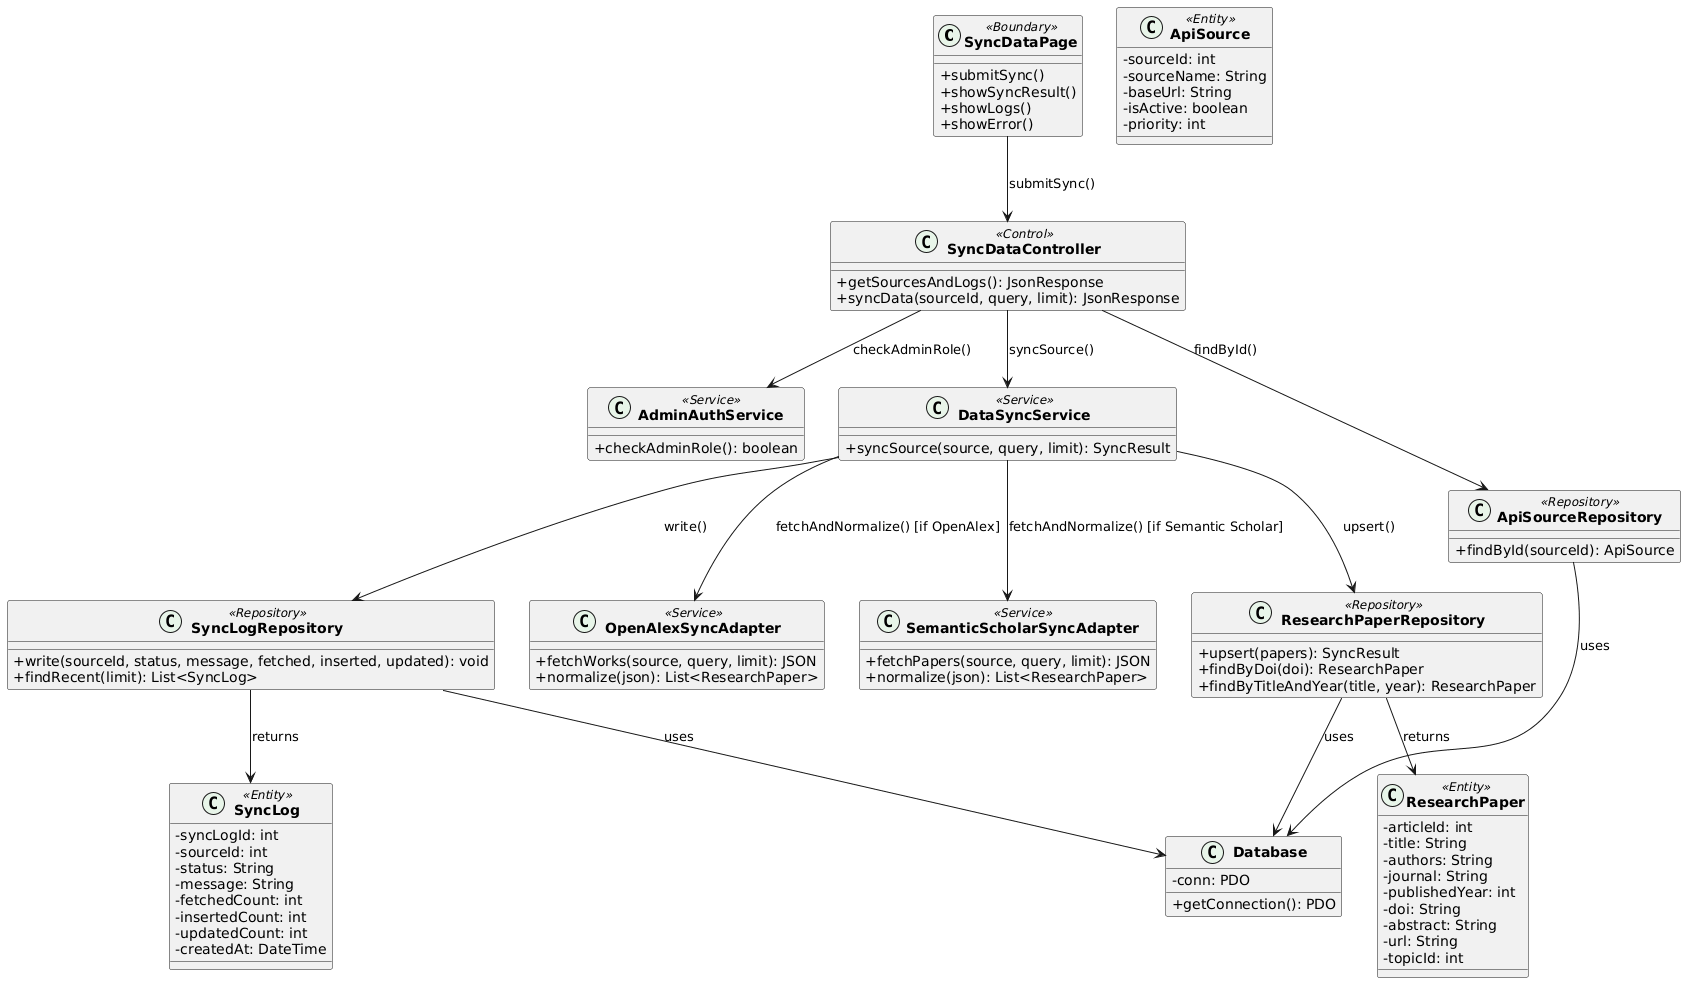
\includegraphics[width=0.8\textwidth]{CDSyncData.png}

	\label{fig:erd}
\end{figure}
\subsubsection{Sequence Diagram}
\begin{figure}[H]
	\centering
	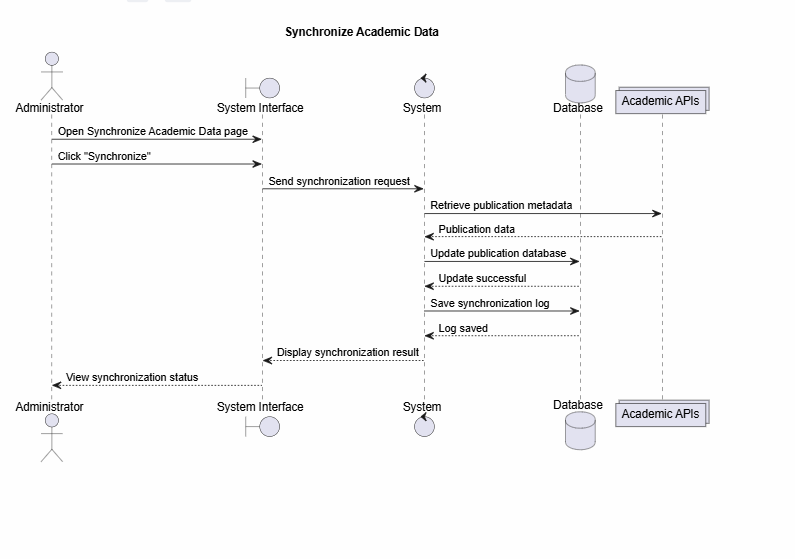
\includegraphics[width=\textwidth]{db.png}

	\label{fig:erd}
\end{figure}


\chapter{\centering\Large\bfseries V SOFTWARE TESTING DOCUMENT}
\addcontentsline{toc}{chapter}{V SOFTWARE TESTING DOCUMENT}


\setcounter{section}{0}
\setcounter{subsection}{0}
\setcounter{subsubsection}{0}

\section{Testing Scope}
The testing scope covers all major functionalities of the Scientific Journal
Publication Trend Tracking System. The following modules and features are included
within the scope of testing:
\begin{itemize}
	\item User Registration
	\item User Login and Authentication
	\item Search Scientific Publications
	\item View Publication Details
	\item Save and Manage Bookmarks
	\item Track Publication Trends
	\item View Statistical Dashboard
	\item Generate Reports 
	\item View Trending Topics
	\item Follow Research Topics
	\item Receive Notifications
	
\end{itemize}
The following features are excluded from the testing scope:
\begin{itemize}
	\item Third-party services and external systems that are outside the project scope.
	\item Real-time publication trend prediction using Artificial Intelligence (AI)
	or Machine Learning (ML) techniques.
	\item Performance testing under extremely large-scale environments involving
	more than 10,000 concurrent users.
\end{itemize}

\section{Test Strategy}
\subsection{Testing Types}
\begin{itemize}
	\item \textbf{Functional Testing:} Verify that all system functions operate according to the specified requirements.
	
	\item \textbf{Integration Testing:} Verify communication and data exchange between the frontend, backend, database, and external APIs.
	
	\item \textbf{System Testing:} Validate complete business workflows and end-to-end system functionality.
	
	\item \textbf{Performance Testing:} Evaluate system response time and behavior under different workloads.
\end{itemize}
\subsection{Testing Levels}
\begin{itemize}
	\item \textbf{Unit Testing:}
	Verify the correctness of individual modules using white-box testing techniques.
	
	\item \textbf{Integration Testing:}
	Verify interactions among integrated components and services.
	
	\item \textbf{System Testing:}
	Validate complete business processes using black-box testing techniques.
	
	\item \textbf{Performance Testing:}
	Observe system behavior and collect performance metrics under different workloads.
\end{itemize}
\subsection{Supporting Tools}

\begin{table}[H]
	\centering
	\begin{tabular}{|p{4cm}|p{8cm}|}
		\hline
		\textbf{Tool} & \textbf{Purpose} \\ \hline
		Visual Studio Code & Application development and source code editing \\ \hline
		MySQL & Database validation and data storage testing \\ \hline
		phpMyAdmin & Database administration and query verification \\ \hline
		Google Chrome & User interface and functional testing \\ \hline
		Postman & API testing and response validation \\ \hline
		GitHub & Source code version control and collaboration \\ \hline
	\end{tabular}
	\label{tab:supporting_tools}
	
\end{table}

\section{Test Plan}
\begin{table}[H]
	\centering
	\begin{tabular}{|p{4cm}|p{8cm}|}
		\hline
		\textbf{Item} & \textbf{Description} \\ \hline
		Environment & Windows 11, WampServer, MySQL \\ \hline
		Browser & Google Chrome \\ \hline
		Database & MySQL \\ \hline
		External APIs & OpenAlex, CrossRef \\ \hline
		Test Period & During system development and before deployment \\ \hline
	\end{tabular}

\end{table}

\subsection{Entry Criteria}
\begin{itemize}
	\item Source code has been completed.
	\item Database configuration has been completed.
	\item External APIs are accessible.
\end{itemize}

\subsection{Exit Criteria}

\begin{itemize}
	\item All major functionalities have been tested.
	\item No critical defects remain unresolved.
\end{itemize}

\section{Test Case}

\begin{table}[H]
	\centering
	\begin{tabular}{|l|c|}
		\hline
		\textbf{Module} & \textbf{Number of Test Cases} \\ \hline
		User Registration & 5 \\ \hline
		User Login & 3 \\ \hline
		Publication Search & 4 \\ \hline
		Bookmarks & 3 \\ \hline
		Follow Research Topics & 3 \\ \hline
		Notifications & 2 \\ \hline
		Publication Trend Analysis & 2 \\ \hline
		\textbf{Total} & \textbf{22} \\ \hline
	\end{tabular}
	
\end{table}

\subsection{User Registration}
\begin{table}[H]
	\centering
	\small
	\begin{tabular}{|p{4cm}|p{10cm}|}
		\hline
		\textbf{Field} & \textbf{Description} \\
		\hline
		
		Module &
		User Registration \\
		\hline
		
		Test Case ID &
		TC\_REG\_01 \\
		\hline
		
		Test Case Name &
		Valid Registration \\
		\hline
		
		Objective &
		Verify that a user can successfully create a new account.\\
		\hline
		
		Preconditions &
		Email and username do not exist in the database.\\
		\hline
		
		Test Data &
		\begin{tabular}[t]{@{}l@{}}
			Full Name: Group Six\\
			Username: Group6\\
			Email: group6@gmail.com\\
			Password: Group654321 
		\end{tabular}
		\\
		\hline
		
		Test Steps &
		\begin{tabular}[t]{@{}l@{}}
			1. Open Registration page.\\
			2. Enter all required information.\\
			3. Click Register.
		\end{tabular}
		\\
		\hline
		
		Expected Result &
		Account is created successfully and saved in the database.\\
		\hline
		
		Actual Result &
		Account created successfully.\\
		\hline
		
		Status &
		Pass \\
		\hline
		
	\end{tabular}

\end{table}


\begin{table}[H]
	\centering
	\small
	\begin{tabular}{|p{4cm}|p{10cm}|}
		\hline
		\textbf{Field} & \textbf{Description} \\
		\hline
		
		Module &
		User Registration \\
		\hline
		
		Test Case ID &
		TC\_REG\_02 \\
		\hline
		
		Test Case Name &
		Empty Required Fields \\
		\hline
		
		Objective &
		Verify validation for mandatory fields. \\
		\hline
		
		Preconditions &
		None \\
		\hline
		
		Test Data &
		All fields are left blank.
		\\
		\hline
		
		Test Steps &
		\begin{tabular}[t]{@{}l@{}}
			1. Open Registration page.\\
			2. Leave all fields empty.\\
			3. Click Register.
		\end{tabular}
		\\
		\hline
		
		Expected Result &
		System displays a validation message requiring all mandatory fields to be filled.
		\\
		\hline
		
		Actual Result &
		Validation message displayed correctly.
		\\
		\hline
		
		Status &
		Pass \\
		\hline
		
	\end{tabular}
	 Fields}
\end{table}


\begin{table}[H]
	\centering
	\small
	\begin{tabular}{|p{4cm}|p{10cm}|}
		\hline
		\textbf{Field} & \textbf{Description} \\
		\hline
		
		Module &
		User Registration \\
		\hline
		
		Test Case ID &
		TC\_REG\_03 \\
		\hline
		
		Test Case Name &
		Invalid Email Format \\
		\hline
		
		Objective &
		Verify email format validation.
		\\
		\hline
		
		Preconditions &
		None
		\\
		\hline
		
		Test Data &
		Email: group6123
		\\
		\hline
		
		Test Steps &
		\begin{tabular}[t]{@{}l@{}}
			1. Open Registration page.\\
			2. Enter an invalid email address.\\
			3. Click Register.
		\end{tabular}
		\\
		\hline
		
		Expected Result &
		System displays "Invalid email address".
		\\
		\hline
		
		Actual Result &
		Validation message displayed correctly.
		\\
		\hline
		
		Status &
		Pass \\
		\hline
		
	\end{tabular}

\end{table}


\begin{table}[H]
	\centering
	\small
	\begin{tabular}{|p{4cm}|p{10cm}|}
		\hline
		\textbf{Field} & \textbf{Description} \\
		\hline
		
		Module &
		User Registration \\
		\hline
		
		Test Case ID &
		TC\_REG\_04 \\
		\hline
		
		Test Case Name &
		Weak Password \\
		\hline
		
		Objective &
		Verify password strength validation.
		\\
		\hline
		
		Preconditions &
		None
		\\
		\hline
		
		Test Data &
		Password: 123456
		\\
		\hline
		
		Test Steps &
		\begin{tabular}[t]{@{}l@{}}
			1. Open Registration page.\\
			2. Enter a weak password.\\
			3. Click Register.
		\end{tabular}
		\\
		\hline
		
		Expected Result &
		System displays a password strength validation message.
		\\
		\hline
		
		Actual Result &
		Validation message displayed correctly.
		\\
		\hline
		
		Status &
		Pass \\
		\hline
		
	\end{tabular}

\end{table}


\begin{table}[H]
	\centering
	\small
	\begin{tabular}{|p{4cm}|p{10cm}|}
		\hline
		\textbf{Field} & \textbf{Description} \\
		\hline
		
		Module &
		User Registration \\
		\hline
		
		Test Case ID &
		TC\_REG\_05 \\
		\hline
		
		Test Case Name &
		Existing Email \\
		\hline
		
		Objective &
		Verify duplicate email validation.
		\\
		\hline
		
		Preconditions &
		The email already exists in the database.
		\\
		\hline
		
		Test Data &
		Email: group6@gmail.com
		\\
		\hline
		
		Test Steps &
		\begin{tabular}[t]{@{}l@{}}
			1. Open Registration page.\\
			2. Enter an existing email.\\
			3. Click Register.
		\end{tabular}
		\\
		\hline
		
		Expected Result &
		System displays "Email already registered".
		\\
		\hline
		
		Actual Result &
		Validation message displayed correctly.
		\\
		\hline
		
		Status &
		Pass \\
		\hline
		
	\end{tabular}
	
\end{table}


\subsection{User Login}
\begin{table}[H]
	\centering
	\small
	\begin{tabular}{|p{4cm}|p{10cm}|}
		\hline
		\textbf{Field} & \textbf{Description} \\
		\hline
		
		Module &
		User Login \\
		\hline
		
		Test Case ID &
		TC\_LOG\_01 \\
		\hline
		
		Test Case Name &
		Successful Login \\
		\hline
		
		Objective &
		Verify that users can log in with valid credentials. \\
		\hline
		
		Preconditions &
		User account exists and is active. \\
		\hline
		
		Test Data &
		\begin{tabular}[t]{@{}l@{}}
			Username: Group6\\
			Password: Group654321
		\end{tabular}
		\\
		\hline
		
		Test Steps &
		\begin{tabular}[t]{@{}l@{}}
			1. Open Login page.\\
			2. Enter valid username and password.\\
			3. Click Login.
		\end{tabular}
		\\
		\hline
		
		Expected Result &
		User is redirected to the dashboard successfully.
		\\
		\hline
		
		Actual Result &
		User logged in successfully.
		\\
		\hline
		
		Status &
		Pass \\
		\hline
	\end{tabular}

\end{table}

\begin{table}[H]
	\centering
	\small
	\begin{tabular}{|p{4cm}|p{10cm}|}
		\hline
		\textbf{Field} & \textbf{Description} \\
		\hline
		
		Module &
		User Login \\
		\hline
		
		Test Case ID &
		TC\_LOG\_02 \\
		\hline
		
		Test Case Name &
		Invalid Login Credentials \\
		\hline
		
		Objective &
		Verify system behavior when username or password is incorrect.
		\\
		\hline
		
		Preconditions &
		User login page is accessible.
		\\
		\hline
		
		Test Data &
		\begin{tabular}[t]{@{}l@{}}
			Scenario 1:\\
			Username: Group6\\
			Password: WrongPassword123\\[2mm]
			
			Scenario 2:\\
			Username: UnknownUser\\
			Password: Group654321
		\end{tabular}
		\\
		\hline
		
		Test Steps &
		\begin{tabular}[t]{@{}l@{}}
			1. Open Login page.\\
			2. Enter invalid credentials.\\
			3. Click Login.
		\end{tabular}
		\\
		\hline
		
		Expected Result &
		System displays ``Invalid username or password''.
		\\
		\hline
		
		Actual Result &
		Error message displayed correctly.
		\\
		\hline
		
		Status &
		Pass \\
		\hline
		
	\end{tabular}

\end{table}

\begin{table}[H]
	\centering
	\small
	\begin{tabular}{|p{4cm}|p{10cm}|}
		\hline
		\textbf{Field} & \textbf{Description} \\
		\hline
		
		Module &
		User Login \\
		\hline
		
		Test Case ID &
		TC\_LOG\_03 \\
		\hline
		
		Test Case Name &
		Empty Credentials \\
		\hline
		
		Objective &
		Verify validation for empty login fields.
		\\
		\hline
		
		Preconditions &
		None.
		\\
		\hline
		
		Test Data &
		Username and Password are empty.
		\\
		\hline
		
		Test Steps &
		\begin{tabular}[t]{@{}l@{}}
			1. Open Login page.\\
			2. Leave all fields blank.\\
			3. Click Login.
		\end{tabular}
		\\
		\hline
		
		Expected Result &
		System displays validation messages for required fields.
		\\
		\hline
		
		Actual Result &
		Validation messages displayed correctly.
		\\
		\hline
		
		Status &
		Pass \\
		\hline
	\end{tabular}

\end{table}

\subsection{Search Scientific Publication}
\begin{table}[H]
	\centering
	\small
	\begin{tabular}{|p{4cm}|p{10cm}|}
		\hline
		\textbf{Field} & \textbf{Description} \\
		\hline
		
		Module &
		Search Publications \\
		\hline
		
		Test Case ID &
		TC\_SEARCH\_01 \\
		\hline
		
		Test Case Name &
		Search by Valid Keyword \\
		\hline
		
		Objective &
		Verify that users can search publications using a valid keyword.
		\\
		\hline
		
		Preconditions &
		Publication data exists in the database.
		\\
		\hline
		
		Test Data &
		Keyword: Machine Learning
		\\
		\hline
		
		Test Steps &
		\begin{tabular}[t]{@{}l@{}}
			1. Enter keyword "Machine Learning".\\
			2. Click Search.
		\end{tabular}
		\\
		\hline
		
		Expected Result &
		A list of relevant publications is displayed.
		\\
		\hline
		
		Actual Result &
		Relevant publications displayed successfully.
		\\
		\hline
		
		Status &
		Pass \\
		\hline
	\end{tabular}

\end{table}

\begin{table}[H]
	\centering
	\small
	\begin{tabular}{|p{4cm}|p{10cm}|}
		\hline
		\textbf{Field} & \textbf{Description} \\
		\hline
		
		Module &
		Search Publications \\
		\hline
		
		Test Case ID &
		TC\_SEARCH\_02 \\
		\hline
		
		Test Case Name &
		Search with No Results \\
		\hline
		
		Objective &
		Verify system behavior when no publication matches the search keyword.
		\\
		\hline
		
		Preconditions &
		System is available.
		\\
		\hline
		
		Test Data &
		Keyword: abcdeftopic123
		\\
		\hline
		
		Test Steps &
		\begin{tabular}[t]{@{}l@{}}
			1. Enter keyword "abcdeftopic123".\\
			2. Click Search.
		\end{tabular}
		\\
		\hline
		
		Expected Result &
		System displays "No publications found".
		\\
		\hline
		
		Actual Result &
		No results displayed correctly.
		\\
		\hline
		
		Status &
		Pass \\
		\hline
	\end{tabular}

\end{table}

\begin{table}[H]
	\centering
	\small
	\begin{tabular}{|p{4cm}|p{10cm}|}
		\hline
		\textbf{Field} & \textbf{Description} \\
		\hline
		
		Module &
		Search Publications \\
		\hline
		
		Test Case ID &
		TC\_SEARCH\_03 \\
		\hline
		
		Test Case Name &
		Filter by Publication Year \\
		\hline
		
		Objective &
		Verify filtering publications by publication year.
		\\
		\hline
		
		Preconditions &
		Publications from multiple years exist.
		\\
		\hline
		
		Test Data &
		Year: 2024
		\\
		\hline
		
		Test Steps &
		\begin{tabular}[t]{@{}l@{}}
			1. Open Search page.\\
			2. Select publication year = 2024.\\
			3. Click Apply Filter.
		\end{tabular}
		\\
		\hline
		
		Expected Result &
		Only publications published in 2024 are displayed.
		\\
		\hline
		
		Actual Result &
		Publications filtered correctly by year.
		\\
		\hline
		
		Status &
		Pass \\
		\hline
	\end{tabular}

\end{table}

\begin{table}[H]
	\centering
	\small
	\begin{tabular}{|p{4cm}|p{10cm}|}
		\hline
		\textbf{Field} & \textbf{Description} \\
		\hline
		
		Module &
		Search Publications \\
		\hline
		
		Test Case ID &
		TC\_SEARCH\_04 \\
		\hline
		
		Test Case Name &
		Filter Open Access Publications \\
		\hline
		
		Objective &
		Verify filtering publications with Open Access status.
		\\
		\hline
		
		Preconditions &
		The database contains both Open Access and non-Open Access publications.
		\\
		\hline
		
		Test Data &
		Open Access = True
		\\
		\hline
		
		Test Steps &
		\begin{tabular}[t]{@{}l@{}}
			1. Open Search page.\\
			2. Enable Open Access filter.\\
			3. Click Apply Filter.
		\end{tabular}
		\\
		\hline
		
		Expected Result &
		Only Open Access publications are displayed.
		\\
		\hline
		
		Actual Result &
		Open Access publications displayed correctly.
		\\
		\hline
		
		Status &
		Pass \\
		\hline
	\end{tabular}

\end{table}

\subsection{Manage Bookmarks}
\begin{table}[H]
	\centering
	\small
	\begin{tabular}{|p{4cm}|p{10cm}|}
		\hline
		\textbf{Field} & \textbf{Description} \\
		\hline
		
		Module &
		Bookmark (Favorites) \\
		\hline
		
		Test Case ID &
		TC\_BM\_01 \\
		\hline
		
		Test Case Name &
		Add Publication to Favorites \\
		\hline
		
		Objective &
		Verify that a publication can be added to the bookmark list successfully.
		\\
		\hline
		
		Preconditions &
		User has logged into the system.
		\\
		\hline
		
		Test Data &
		Publication: ``Deep Learning in Healthcare''
		\\
		\hline
		
		Test Steps &
		\begin{tabular}[t]{@{}l@{}}
			1. Search for publication ``Deep Learning in Healthcare''.\\
			2. Open the publication details page.\\
			3. Click the Bookmark button.
		\end{tabular}
		\\
		\hline
		
		Expected Result &
		The publication is added to the bookmark table successfully.
		\\
		\hline
		
		Actual Result &
		Bookmark added successfully.
		\\
		\hline
		
		Status &
		Pass \\
		\hline
	\end{tabular}

\end{table}

\begin{table}[H]
	\centering
	\small
	\begin{tabular}{|p{4cm}|p{10cm}|}
		\hline
		\textbf{Field} & \textbf{Description} \\
		\hline
		
		Module &
		Bookmark (Favorites) \\
		\hline
		
		Test Case ID &
		TC\_BM\_02 \\
		\hline
		
		Test Case Name &
		Add Duplicate Bookmark \\
		\hline
		
		Objective &
		Verify that duplicate bookmarks are not created.
		\\
		\hline
		
		Preconditions &
		The publication has already been bookmarked.
		\\
		\hline
		
		Test Data &
		Publication: ``Deep Learning in Healthcare''
		\\
		\hline
		
		Test Steps &
		\begin{tabular}[t]{@{}l@{}}
			1. Open the details page of a bookmarked publication.\\
			2. Click the Bookmark button again.
		\end{tabular}
		\\
		\hline
		
		Expected Result &
		System displays ``This publication is already in your favorites'' and no duplicate record is created.
		\\
		\hline
		
		Actual Result &
		Message displayed correctly and no duplicate record created.
		\\
		\hline
		
		Status &
		Pass \\
		\hline
	\end{tabular}

\end{table}

\begin{table}[H]
	\centering
	\small
	\begin{tabular}{|p{4cm}|p{10cm}|}
		\hline
		\textbf{Field} & \textbf{Description} \\
		\hline
		
		Module &
		Bookmark (Favorites) \\
		\hline
		
		Test Case ID &
		TC\_BM\_03 \\
		\hline
		
		Test Case Name &
		Remove Bookmark \\
		\hline
		
		Objective &
		Verify the bookmark removal functionality.
		\\
		\hline
		
		Preconditions &
		At least one publication exists in the bookmark list.
		\\
		\hline
		
		Test Data &
		Bookmark ID: 2
		\\
		\hline
		
		Test Steps &
		\begin{tabular}[t]{@{}l@{}}
			1. Open the Favorites page.\\
			2. Select the publication with Bookmark ID = 2.\\
			3. Click the Remove button.
		\end{tabular}
		\\
		\hline
		
		Expected Result &
		The publication is removed from the bookmark list.
		\\
		\hline
		
		Actual Result &
		Bookmark removed successfully.
		\\
		\hline
		
		Status &
		Pass \\
		\hline
	\end{tabular}

\end{table}

\subsection{View Trending Topics}
\begin{table}[H]
	\centering
	\small
	\begin{tabular}{|p{4cm}|p{10cm}|}
		\hline
		\textbf{Field} & \textbf{Description} \\
		\hline
		
		Module &
		Topic Following \\
		\hline
		
		Test Case ID &
		TC\_TOPIC\_01 \\
		\hline
		
		Test Case Name &
		Follow New Topic \\
		\hline
		
		Objective &
		Verify that users can successfully follow a new research topic.
		\\
		\hline
		
		Preconditions &
		User has logged into the system.
		\\
		\hline
		
		Test Data &
		Topic: Artificial Intelligence
		\\
		\hline
		
		Test Steps &
		\begin{tabular}[t]{@{}l@{}}
			1. Open the Trend Topics page.\\
			2. Select topic "Artificial Intelligence".\\
			3. Click the Follow button.
		\end{tabular}
		\\
		\hline
		
		Expected Result &
		The topic is stored in the UserFollowTopic table and a new notification is created.
		\\
		\hline
		
		Actual Result &
		Topic followed successfully and notification created.
		\\
		\hline
		
		Status &
		Pass \\
		\hline
		
	\end{tabular}

\end{table}

\begin{table}[H]
	\centering
	\small
	\begin{tabular}{|p{4cm}|p{10cm}|}
		\hline
		\textbf{Field} & \textbf{Description} \\
		\hline
		
		Module &
		Topic Following \\
		\hline
		
		Test Case ID &
		TC\_TOPIC\_02 \\
		\hline
		
		Test Case Name &
		Follow Existing Topic \\
		\hline
		
		Objective &
		Verify that duplicate topic subscriptions are not created.
		\\
		\hline
		
		Preconditions &
		The topic has already been followed previously.
		\\
		\hline
		
		Test Data &
		Topic: Artificial Intelligence
		\\
		\hline
		
		Test Steps &
		\begin{tabular}[t]{@{}l@{}}
			1. Select topic "Artificial Intelligence".\\
			2. Click the Follow button again.
		\end{tabular}
		\\
		\hline
		
		Expected Result &
		System displays "You are already following this topic" and no new record is created.
		\\
		\hline
		
		Actual Result &
		Correct message displayed and no duplicate record created.
		\\
		\hline
		
		Status &
		Pass \\
		\hline
		
	\end{tabular}

\end{table}
\begin{table}[H]
	\centering
	\small
	\begin{tabular}{|p{4cm}|p{10cm}|}
		\hline
		\textbf{Field} & \textbf{Description} \\
		\hline
		
		Module &
		Topic Following \\
		\hline
		
		Test Case ID &
		TC\_TOPIC\_03 \\
		\hline
		
		Test Case Name &
		Unfollow Topic \\
		\hline
		
		Objective &
		Verify that users can successfully unfollow a topic.
		\\
		\hline
		
		Preconditions &
		The topic is currently being followed by the user.
		\\
		\hline
		
		Test Data &
		Topic: Artificial Intelligence
		\\
		\hline
		
		Test Steps &
		\begin{tabular}[t]{@{}l@{}}
			1. Open the Followed Topics list.\\
			2. Select topic "Artificial Intelligence".\\
			3. Click the Unfollow button.
		\end{tabular}
		\\
		\hline
		
		Expected Result &
		The topic is removed from the UserFollowTopic table.
		\\
		\hline
		
		Actual Result &
		Topic unfollowed successfully.
		\\
		\hline
		
		Status &
		Pass \\
		\hline
		
	\end{tabular}

\end{table}

\subsection{Notification Management}
\begin{table}[H]
	\centering
	\small
	\begin{tabular}{|p{4cm}|p{10cm}|}
		\hline
		\textbf{Field} & \textbf{Description} \\
		\hline
		
		Module &
		Notification Management \\
		\hline
		
		Test Case ID &
		TC\_NOTI\_01 \\
		\hline
		
		Test Case Name &
		View Notification List \\
		\hline
		
		Objective &
		Verify that users can view all notifications associated with their account.
		\\
		\hline
		
		Preconditions &
		User has logged into the system and has at least one notification.
		\\
		\hline
		
		Test Data &
		User ID: 1
		\\
		\hline
		
		Test Steps &
		\begin{tabular}[t]{@{}l@{}}
			1. Log in to the system.\\
			2. Click the Notification icon.\\
			3. Open the Notification page.
		\end{tabular}
		\\
		\hline
		
		Expected Result &
		The system displays all notifications belonging to the user, including title, content, and status.
		\\
		\hline
		
		Actual Result &
		Notification list displayed successfully.
		\\
		\hline
		
		Status &
		Pass \\
		\hline
		
	\end{tabular}

\end{table}

\begin{table}[H]
	\centering
	\small
	\begin{tabular}{|p{4cm}|p{10cm}|}
		\hline
		\textbf{Field} & \textbf{Description} \\
		\hline
		
		Module &
		Notification Management \\
		\hline
		
		Test Case ID &
		TC\_NOTI\_02 \\
		\hline
		
		Test Case Name &
		Mark Notification as Read \\
		\hline
		
		Objective &
		Verify that users can mark a notification as read.
		\\
		\hline
		
		Preconditions &
		User has at least one unread notification.
		\\
		\hline
		
		Test Data &
		Notification ID: 5
		\\
		\hline
		
		Test Steps &
		\begin{tabular}[t]{@{}l@{}}
			1. Open the Notification page.\\
			2. Select an unread notification.\\
			3. Click the notification to view details.
		\end{tabular}
		\\
		\hline
		
		Expected Result &
		The notification status changes from ``Unread'' to ``Read''.
		\\
		\hline
		
		Actual Result &
		Notification status updated successfully.
		\\
		\hline
		
		Status &
		Pass \\
		\hline
		
	\end{tabular}

\end{table}

\subsection{Trend Analysis}
\begin{table}[H]
	\centering
	\small
	\begin{tabular}{|p{4cm}|p{10cm}|}
		\hline
		\textbf{Field} & \textbf{Description} \\
		\hline
		
		Module &
		Trend Analysis \\
		\hline
		
		Test Case ID &
		TC\_TREND\_01 \\
		\hline
		
		Test Case Name &
		Successful Trend Analysis \\
		\hline
		
		Objective &
		Verify that the system correctly generates publication trend analysis for a valid research topic based on synchronized publication metadata stored in the database.
		\\
		\hline
		
		Preconditions &
		Publication metadata for the topic "Machine Learning" has been synchronized into the database from Semantic Scholar, OpenAlex, and Crossref.	
		\\
		\hline
		
		Test Data &
		\begin{tabular}[t]{@{}l@{}}
			Topic: Machine Learning\\
			Year From: 2020\\
			Year To: 2024
		\end{tabular}
		\\
		\hline
		
		Test Steps &
		\begin{tabular}[t]{@{}l@{}}
			1. Log in to the system.\\
			2. Access "Track Publication Trends".\\
			3. Enter topic "Machine Learning".\\
			4. Select year range from 2020 to 2024.\\
			5. Click Analyze.
		\end{tabular}
		\\
		\hline
		
		Expected Result &
		The system aggregates publication counts by year from the database, calculates growth rate, and displays trend statistics and visual charts showing increasing or decreasing publication activity.
		\\
		\hline
		
		Actual Result &
		Trend analysis results displayed correctly.
		\\
		\hline
		
		Status &
		Pass \\
		\hline
		
	\end{tabular}

\end{table}

\begin{table}[H]
	\centering
	\small
	\begin{tabular}{|p{4cm}|p{10cm}|}
		\hline
		\textbf{Field} & \textbf{Description} \\
		\hline
		
		Module &
		Trend Analysis \\
		\hline
		
		Test Case ID &
		TC\_TREND\_02 \\
		\hline
		
		Test Case Name &
		Trend Analysis with No Data \\
		\hline
		
		Objective &
		Verify system behavior when no trend data is available.
		\\
		\hline
		
		Preconditions &
		System is available and database contains no matching publication data for the topic
		\\
		\hline
		
		Test Data &
		Topic: abcdeftopic
		\\
		\hline
		
		Test Steps &
		\begin{tabular}[t]{@{}l@{}}
			1. Enter non-existing topic "abcdeftopic".\\
			2. Click Analyze.
		\end{tabular}
		\\
		\hline
		
		Expected Result &
		An empty result list is displayed and no system error occurs.
		\\
		\hline
		
		Actual Result &
		Empty result list displayed correctly.
		\\
		\hline
		
		Status &
		Pass \\
		\hline
		
	\end{tabular}

\end{table}
\subsection{Admin Management}
\begin{longtable}{|p{4cm}|p{10cm}|}
	\hline
	\textbf{Field} & \textbf{Description} \\ \hline
	Module & Admin - User Management \\ \hline
	Test Case ID & TC\_ADMIN\_01 \\ \hline
	Test Case Name & Lock User Account \\ \hline
	Objective & Verify that admin can lock an active user account. \\ \hline
	Preconditions & Admin is logged in. User account exists and has active status. \\ \hline
	Test Data & User ID: 2 \newline Action: lock \\ \hline
	Test Steps &
	1. Open Admin page. \newline
	2. Go to User Management. \newline
	3. Select an active user. \newline
	4. Click Lock. \\ \hline
	Expected Result & User status is updated to locked. \\ \hline
	Actual Result & User account locked successfully. \\ \hline
	Status & Pass \\ \hline
\end{longtable}
\subsection{Add New Topic}
\begin{longtable}{|p{4cm}|p{10cm}|}
	\hline
	\textbf{Field} & \textbf{Description} \\ \hline
	
	Module & Admin - Topic Management \\ \hline
	
	Test Case ID & TC\_ADMIN\_02 \\ \hline
	
	Test Case Name & Add New Topic \\ \hline
	
	Objective &
	Verify that the administrator can successfully add a new topic to the system. \\ \hline
	
	Preconditions &
	Administrator has logged into the Admin page successfully. \\ \hline
	
	Test Data &
	Topic Name: Artificial Intelligence \newline
	Description: Research papers related to artificial intelligence, machine learning, and deep learning.
	\\ \hline
	
	Test Steps &
	1. Open the Admin page. \newline
	2. Navigate to the \textbf{Topic Management} section. \newline
	3. Enter ``Artificial Intelligence'' in the \textbf{Topic Name} field. \newline
	4. Enter ``Research papers related to artificial intelligence, machine learning, and deep learning.'' in the \textbf{Description} field. \newline
	5. Click the \textbf{Add Topic} button.
	\\ \hline
	
	Expected Result &
	The new topic is successfully created and displayed in the Topic List with its ID, topic name, description, and available actions. \\ \hline
	
	Actual Result &
	The topic was added successfully and appeared in the Topic List. \\ \hline
	
	Status & Pass \\ \hline
	
\end{longtable}
\subsection{Edit Existing Topic}
\begin{longtable}{|p{4cm}|p{10cm}|}
	\hline
	\textbf{Field} & \textbf{Description} \\ \hline
	
	Module & Admin - Topic Management \\ \hline
	
	Test Case ID & TC\_ADMIN\_03 \\ \hline
	
	Test Case Name & Update Topic \\ \hline
	
	Objective &
	Verify that the administrator can update an existing topic with topicId, topicName, and description. \\ \hline
	
	Preconditions &
	Administrator has logged into the Admin page successfully. \newline
	At least one topic exists in the topic list.
	\\ \hline
	
	Test Data &
	topicId: 1 \newline
	topicName: Artificial Intelligence and Machine Learning \newline
	description: Research papers related to AI, machine learning, and deep learning.
	\\ \hline
	
	Test Steps &
	1. Open the Admin page. \newline
	2. Go to the Topic Management section. \newline
	3. Select an existing topic. \newline
	4. Update the topic name. \newline
	5. Update the topic description. \newline
	6. Submit the update action.
	\\ \hline
	
	Expected Result &
	The selected topic is updated successfully. The system returns the message ``Topic updated successfully.'' \\ \hline
	
	Actual Result &
	The topic was updated successfully. \\ \hline
	
	Status & Pass \\ \hline
	
\end{longtable}
\subsection{Delete Topic}
\begin{longtable}{|p{4cm}|p{10cm}|}
	\hline
	\textbf{Field} & \textbf{Description} \\ \hline
	
	Module & Admin - Topic Management \\ \hline
	
	Test Case ID & TC\_ADMIN\_04 \\ \hline
	
	Test Case Name & Delete Topic \\ \hline
	
	Objective &
	Verify that the administrator can delete an existing topic with topicId. \\ \hline
	
	Preconditions &
	Administrator has logged into the Admin page successfully. \newline
	At least one topic exists in the topic list.
	\\ \hline
	
	Test Data &
	topicId: 1
	\\ \hline
	
	Test Steps &
	1. Open the Admin page. \newline
	2. Go to the Topic Management section. \newline
	3. Select an existing topic. \newline
	4. Submit the delete action.
	\\ \hline
	
	Expected Result &
	The selected topic is deleted successfully. The system returns the message ``Topic deleted successfully.'' \\ \hline
	
	Actual Result &
	The topic was deleted successfully. \\ \hline
	
	Status & Pass \\ \hline
	
\end{longtable}
\subsection{Create API Source}
\begin{longtable}{|p{4cm}|p{10cm}|}
	\hline
	\textbf{Field} & \textbf{Description} \\ \hline
	
	Module & Admin - API Source Management \\ \hline
	
	Test Case ID & TC\_ADMIN\_05 \\ \hline
	
	Test Case Name & Add API Source \\ \hline
	
	Objective &
	Verify that the administrator can create a new API source with sourceName, baseUrl, description, isActive, and priority. \\ \hline
	
	Preconditions &
	Administrator has logged into the Admin page successfully.
	\\ \hline
	
	Test Data &
	sourceName: OpenAlex \newline
	baseUrl: https://api.openalex.org \newline
	description: OpenAlex API source \newline
	isActive: 1 \newline
	priority: 1
	\\ \hline
	
	Test Steps &
	1. Open the Admin page. \newline
	2. Go to the API Source Management section. \newline
	3. Enter the source name. \newline
	4. Enter the base URL. \newline
	5. Enter the description. \newline
	6. Set the active status. \newline
	7. Enter the priority. \newline
	8. Submit the create action.
	\\ \hline
	
	Expected Result &
	The new API source is created successfully. The system returns the message ``API source added successfully.'' \\ \hline
	
	Actual Result &
	The API source was added successfully. \\ \hline
	
	Status & Pass \\ \hline
	
\end{longtable}
\subsection{Update API Source}
\begin{longtable}{|p{4cm}|p{10cm}|}
	\hline
	\textbf{Field} & \textbf{Description} \\ \hline
	
	Module & Admin - API Source Management \\ \hline
	
	Test Case ID & TC\_ADMIN\_06 \\ \hline
	
	Test Case Name & Update API Source \\ \hline
	
	Objective &
	Verify that the administrator can update an existing API source with sourceId, sourceName, baseUrl, description, isActive, and priority. \\ \hline
	
	Preconditions &
	Administrator has logged into the Admin page successfully. \newline
	At least one API source exists in the API source list.
	\\ \hline
	
	Test Data &
	sourceId: 1 \newline
	sourceName: OpenAlex \newline
	baseUrl: https://api.openalex.org \newline
	description: OpenAlex API source updated \newline
	isActive: 1 \newline
	priority: 2
	\\ \hline
	
	Test Steps &
	1. Open the Admin page. \newline
	2. Go to the API Source Management section. \newline
	3. Select an existing API source. \newline
	4. Update the source name. \newline
	5. Update the base URL. \newline
	6. Update the description. \newline
	7. Update the active status. \newline
	8. Update the priority. \newline
	9. Submit the update action.
	\\ \hline
	
	Expected Result &
	The selected API source is updated successfully. The system returns the message ``API source updated successfully.'' \\ \hline
	
	Actual Result &
	The API source was updated successfully. \\ \hline
	
	Status & Pass \\ \hline
	
\end{longtable}

\subsection{Toggle API Source Status}
\begin{longtable}{|p{4cm}|p{10cm}|}
	\hline
	\textbf{Field} & \textbf{Description} \\ \hline
	
	Module & Admin - API Source Management \\ \hline
	
	Test Case ID & TC\_ADMIN\_07 \\ \hline
	
	Test Case Name & Toggle API Source Status \\ \hline
	
	Objective &
	Verify that the administrator can change the active status of an API source with sourceId. \\ \hline
	
	Preconditions &
	Administrator has logged into the Admin page successfully. \newline
	At least one API source exists in the API source list.
	\\ \hline
	
	Test Data &
	sourceId: 1
	\\ \hline
	
	Test Steps &
	1. Open the Admin page. \newline
	2. Go to the API Source Management section. \newline
	3. Select an existing API source. \newline
	4. Submit the toggle action.
	\\ \hline
	
	Expected Result &
	The selected API source status is changed successfully. The system returns the message ``API source status changed successfully.'' \\ \hline
	
	Actual Result &
	The API source status was changed successfully. \\ \hline
	
	Status & Pass \\ \hline
	
\end{longtable}
\subsection{Delete API Source}
\begin{longtable}{|p{4cm}|p{10cm}|}
	\hline
	\textbf{Field} & \textbf{Description} \\ \hline
	
	Module & Admin - API Source Management \\ \hline
	
	Test Case ID & TC\_ADMIN\_08 \\ \hline
	
	Test Case Name & Delete API Source \\ \hline
	
	Objective &
	Verify that the administrator can delete an existing API source with sourceId. \\ \hline
	
	Preconditions &
	Administrator has logged into the Admin page successfully. \newline
	At least one API source exists in the API source list.
	\\ \hline
	
	Test Data &
	sourceId: 1
	\\ \hline
	
	Test Steps &
	1. Open the Admin page. \newline
	2. Go to the API Source Management section. \newline
	3. Select an existing API source. \newline
	4. Submit the delete action.
	\\ \hline
	
	Expected Result &
	The selected API source is deleted successfully. The system returns the message ``API source deleted successfully.'' \\ \hline
	
	Actual Result &
	The API source was deleted successfully. \\ \hline
	
	Status & Pass \\ \hline
	
\end{longtable}
\subsection{Synchronize Data From API}
\begin{longtable}{|p{4cm}|p{10cm}|}
	\hline
	\textbf{Field} & \textbf{Description} \\ \hline
	
	Module & Admin - API Synchronization \\ \hline
	
	Test Case ID & TC\_ADMIN\_09 \\ \hline
	
	Test Case Name & Synchronize Data From API \\ \hline
	
	Objective &
	Verify that the administrator can synchronize data from an active API source with sourceId, query, and limit. \\ \hline
	
	Preconditions &
	Administrator has logged into the Admin page successfully. \newline
	At least one active API source exists.
	\\ \hline
	
	Test Data &
	sourceId: 1 \newline
	query: science research \newline
	limit: 10
	\\ \hline
	
	Test Steps &
	1. Open the Admin page. \newline
	2. Go to the API Synchronization section. \newline
	3. Select an active API source. \newline
	4. Enter the query. \newline
	5. Enter the limit. \newline
	6. Submit the synchronization action.
	\\ \hline
	
	Expected Result &
	The data is synchronized successfully. The system returns the message ``Synchronization completed successfully.'' \\ \hline
	
	Actual Result &
	The data was synchronized successfully. \\ \hline
	
	Status & Pass \\ \hline
	
\end{longtable}
\subsection{Add Research Paper}
\begin{longtable}{|p{4cm}|p{10cm}|}
	\hline
	\textbf{Field} & \textbf{Description} \\ \hline
	
	Module & Admin - Paper Management \\ \hline
	
	Test Case ID & TC\_ADMIN\_10 \\ \hline
	
	Test Case Name & Add Research Paper \\ \hline
	
	Objective &
	Verify that the administrator can create a new research paper with title, authors, journal, publishedYear, doi, abstract, url, and topicId. \\ \hline
	
	Preconditions &
	Administrator has logged into the Admin page successfully.
	\\ \hline
	
	Test Data &
	title: Deep Learning for Scientific Publication Analysis \newline
	authors: Nguyen Van A \newline
	journal: AI Journal \newline
	publishedYear: 2025 \newline
	doi: 10.1000/test001 \newline
	abstract: Research paper abstract \newline
	url: https://example.com/paper \newline
	topicId: 1
	\\ \hline
	
	Test Steps &
	1. Open the Admin page. \newline
	2. Go to the Paper Management section. \newline
	3. Enter the title. \newline
	4. Enter the authors. \newline
	5. Enter the journal. \newline
	6. Enter the published year. \newline
	7. Enter the DOI. \newline
	8. Enter the abstract. \newline
	9. Enter the URL. \newline
	10. Select the topic. \newline
	11. Submit the create action.
	\\ \hline
	
	Expected Result &
	The new research paper is created successfully. The system returns the message ``Research paper added successfully.'' \\ \hline
	
	Actual Result &
	The research paper was added successfully. \\ \hline
	
	Status & Pass \\ \hline
	
\end{longtable}
\subsection{Update Research Paper}
\begin{longtable}{|p{4cm}|p{10cm}|}
	\hline
	\textbf{Field} & \textbf{Description} \\ \hline
	
	Module & Admin - Paper Management \\ \hline
	
	Test Case ID & TC\_ADMIN\_11 \\ \hline
	
	Test Case Name & Update Research Paper \\ \hline
	
	Objective &
	Verify that the administrator can update an existing research paper with articleId, title, authors, journal, publishedYear, doi, abstract, url, and topicId. \\ \hline
	
	Preconditions &
	Administrator has logged into the Admin page successfully. \newline
	At least one research paper exists in the paper list.
	\\ \hline
	
	Test Data &
	articleId: 1 \newline
	title: Updated Deep Learning for Scientific Publication Analysis \newline
	authors: Nguyen Van A \newline
	journal: AI Journal \newline
	publishedYear: 2025 \newline
	doi: 10.1000/test001 \newline
	abstract: Updated research paper abstract \newline
	url: https://example.com/paper \newline
	topicId: 1
	\\ \hline
	
	Test Steps &
	1. Open the Admin page. \newline
	2. Go to the Paper Management section. \newline
	3. Select an existing research paper. \newline
	4. Update the title. \newline
	5. Update the authors. \newline
	6. Update the journal. \newline
	7. Update the published year. \newline
	8. Update the DOI. \newline
	9. Update the abstract. \newline
	10. Update the URL. \newline
	11. Update the topic. \newline
	12. Submit the update action.
	\\ \hline
	
	Expected Result &
	The selected research paper is updated successfully. The system returns the message ``Research paper updated successfully.'' \\ \hline
	
	Actual Result &
	The research paper was updated successfully. \\ \hline
	
	Status & Pass \\ \hline
	
\end{longtable}
\subsection{Delete Research Paper}
\begin{longtable}{|p{4cm}|p{10cm}|}
	\hline
	\textbf{Field} & \textbf{Description} \\ \hline
	
	Module & Admin - Paper Management \\ \hline
	
	Test Case ID & TC\_ADMIN\_12 \\ \hline
	
	Test Case Name & Delete Research Paper \\ \hline
	
	Objective &
	Verify that the administrator can delete an existing research paper with articleId. \\ \hline
	
	Preconditions &
	Administrator has logged into the Admin page successfully. \newline
	At least one research paper exists in the paper list.
	\\ \hline
	
	Test Data &
	articleId: 1
	\\ \hline
	
	Test Steps &
	1. Open the Admin page. \newline
	2. Go to the Paper Management section. \newline
	3. Select an existing research paper. \newline
	4. Submit the delete action.
	\\ \hline
	
	Expected Result &
	The selected research paper is deleted successfully. The system returns the message ``Research paper deleted successfully.'' \\ \hline
	
	Actual Result &
	The research paper was deleted successfully. \\ \hline
	
	Status & Pass \\ \hline
	
\end{longtable}
\subsection{Create Notification For One User}
\begin{longtable}{|p{4cm}|p{10cm}|}
	\hline
	\textbf{Field} & \textbf{Description} \\ \hline
	
	Module & Admin - Notification Management \\ \hline
	
	Test Case ID & TC\_ADMIN\_13 \\ \hline
	
	Test Case Name & Create Notification For One User \\ \hline
	
	Objective &
	Verify that the administrator can create a notification for one user with title, content, type, link, and userId. \\ \hline
	
	Preconditions &
	Administrator has logged into the Admin page successfully. \newline
	At least one user exists in the user list.
	\\ \hline
	
	Test Data &
	title: System Notice \newline
	content: This is a system notification. \newline
	type: system \newline
	link: https://example.com \newline
	userId: 1 \newline
	sendAll: 0
	\\ \hline
	
	Test Steps &
	1. Open the Admin page. \newline
	2. Go to the Notification Management section. \newline
	3. Enter the title. \newline
	4. Enter the content. \newline
	5. Enter the type. \newline
	6. Enter the link. \newline
	7. Select a user. \newline
	8. Submit the create action.
	\\ \hline
	
	Expected Result &
	The notification is created successfully. The system returns the message ``Notification created successfully.'' \\ \hline
	
	Actual Result &
	The notification was created successfully. \\ \hline
	
	Status & Pass \\ \hline
	
\end{longtable}
\subsection{Create Notification For All Active Users}
\begin{longtable}{|p{4cm}|p{10cm}|}
	\hline
	\textbf{Field} & \textbf{Description} \\ \hline
	
	Module & Admin - Notification Management \\ \hline
	
	Test Case ID & TC\_ADMIN\_14 \\ \hline
	
	Test Case Name & Create Notification For All Active Users \\ \hline
	
	Objective &
	Verify that the administrator can create a notification for all active users with title, content, type, link, and sendAll. \\ \hline
	
	Preconditions &
	Administrator has logged into the Admin page successfully. \newline
	At least one active user exists in the user list.
	\\ \hline
	
	Test Data &
	title: System Notice \newline
	content: This is a system notification for all active users. \newline
	type: system \newline
	link: https://example.com \newline
	sendAll: 1
	\\ \hline
	
	Test Steps &
	1. Open the Admin page. \newline
	2. Go to the Notification Management section. \newline
	3. Enter the title. \newline
	4. Enter the content. \newline
	5. Enter the type. \newline
	6. Enter the link. \newline
	7. Select send all. \newline
	8. Submit the create action.
	\\ \hline
	
	Expected Result &
	The notification is created successfully for all active users. The system returns the message ``Notification sent to all users.'' \\ \hline
	
	Actual Result &
	The notification was created successfully for all active users. \\ \hline
	
	Status & Pass \\ \hline
	
\end{longtable}


\chapter{\centering\Large\bfseries VI . RELEASE PACKAGE AND USER GUIDE}
\addcontentsline{toc}{chapter}{VI . RELEASE PACKAGE AND USER GUIDE}
\setcounter{section}{0}
\section{ Deliverable Package}



% ── Pastel pink color definitions ──
\definecolor{pinkheader}{RGB}{244, 194, 199}   % darker pink for header
\definecolor{pinkrow}{RGB}{253, 235, 237}       % light pink for alternate rows
\definecolor{pinkborder}{RGB}{230, 160, 170}    % pink border

% Column type: top-aligned, auto-wrapping text
\newcolumntype{L}[1]{>{\raggedright\arraybackslash}p{#1}}


	
	\renewcommand{\arraystretch}{1.3}
	\arrayrulecolor{pinkborder}
	
	\begin{table}[htbp]
		\centering
	
		\begin{tabularx}{\textwidth}{|c|L{3cm}|X|}
			\hline
			\rowcolor{pinkheader}
			\textbf{\#} & \textbf{Deliverable Item} & \textbf{Description} \\
			\hline
			
			1 & Schedule/Task Tracking &
			We use Jira to track our development progress and manage sprints/tasks, and Confluence to store documentation, meeting notes, and feature specifications.
			\begin{itemize}[leftmargin=*, itemsep=0pt, topsep=2pt]
				\item Jira
				\item Confluence
			\end{itemize} \\
			\hline
			
			\rowcolor{pinkrow}
			2 & Project BackLogs &
			Jira is used to organize the backlog as boards/lists, grouped by the main modules: Paper Search, Trend Analysis, Follow Topic, Bookmark, and System Administration. \\
			\hline
			
			3 & Source code &
			We host the full frontend and backend source code on GitHub.
			
			GitHub repository link: \url{https://github.com/NguyenNgocBaoTram10/Scientific-Journal-Publication-Trend-Tracking-System}
			\begin{itemize}[leftmargin=*, itemsep=0pt, topsep=2pt]
				\item Frontend (\texttt{source\_code/page})
				\item Backend (\texttt{source\_code/api})
				\item Config (\texttt{source\_code/config})
			\end{itemize} \\
			\hline
			
			\rowcolor{pinkrow}
			4 & Data Script &
			N/A -- the system does not use a static data-loading script; paper data is fetched in real time from the OpenAlex API (primary source) and the Crossref API (fallback source when OpenAlex fails). \\
			\hline
			
			5 & Final Project Report Document &
			A document that consolidates the project report (requirement specification, analysis and design, use case/class/sequence/ERD diagrams, etc.), authored in LaTeX (\texttt{main.tex}) and compiled to \texttt{main.pdf}. \\
			\hline
			
			\rowcolor{pinkrow}
			6 & Test Case Document &
			A document that outlines the test cases required for validating each core feature of the project: paper search (including the OpenAlex $\rightarrow$ Crossref fallback), save/remove bookmark, follow topic, receive notifications, generate reports, and admin functions. \\
			\hline
			
		\end{tabularx}
	\end{table}
	


\section{  Installation Guide}

\subsection{Back end}
{\arrayrulecolor{yellowborder}
	\begin{table}[H]
		\centering
		
		\begin{tabularx}{\textwidth}{|c|X|}
			\hline
			\rowcolor{yellowheader}
			\textbf{Step} & \textbf{Description} \\
			\hline
			
			1 & Download and install a local server stack (XAMPP or WAMP) -- this bundles Apache, PHP, and MySQL: \url{https://www.apachefriends.org/download.html} \\
			\hline
			
			\rowcolor{yellowrow}
			2 & Download and install Git: \url{https://git-scm.com/downloads} \\
			\hline
			
			3 & Download and install Visual Studio Code: \url{https://code.visualstudio.com/download} \\
			\hline
			
			\rowcolor{yellowrow}
			4 & Navigate to the server's web root folder (e.g. \texttt{C:\textbackslash xampp\textbackslash htdocs} or \texttt{C:\textbackslash wamp64\textbackslash www}), click the address bar, type \texttt{cmd} and press Enter. \\
			\hline
			
			5 & Open a new terminal in Visual Studio Code and type this command:
			
			git clone \url{https://github.com/NguyenNgocBaoTram10/Scientific-Journal-Publication-Trend-Tracking-System.git} \\
			\hline
			
			\rowcolor{yellowrow}
			6 & Start \textbf{Apache} and \textbf{MySQL} from the XAMPP/WAMP control panel. \\
			\hline
			
			7 & Open \texttt{http://localhost/phpmyadmin}, create a new database named \textbf{\texttt{sjptts}}, and import the project's SQL schema (if provided) or create the tables matching \texttt{source\_code/config/database.php}. \\
			\hline
			
			\rowcolor{yellowrow}
			8 & Make sure PHP's \textbf{cURL} extension is enabled (required to call the OpenAlex/Crossref APIs) -- this is usually enabled by default in XAMPP/WAMP. \\
			\hline
			
		\end{tabularx}
	\end{table}
}


\subsection{Frontend}

{\arrayrulecolor{blueborder}
\begin{table}[H]
		\centering
		
		\begin{tabularx}{\textwidth}{|c|X|}
			\hline
			\rowcolor{blueheader}
			\textbf{Step} & \textbf{Description} \\
			\hline
			
			1 & The front end is plain HTML/CSS (Tailwind via CDN) and vanilla JavaScript -- \textbf{no Node.js or npm install is required}. \\
			\hline
			
			\rowcolor{bluerow}
			2 & Open your Visual Studio Code. \\
			\hline
			
			3 & Click \textbf{File} and choose \textbf{Add folder to workspace}. \\
			\hline
			
			\rowcolor{bluerow}
			4 & Choose the project folder (\texttt{source\_code/page}) and click \textbf{Add}. \\
			\hline
			
			5 & Since the pages call the backend via relative paths (e.g. \texttt{../api/timkiem.php}), the project must be served through Apache -- open your browser and go to:
			
			\url{http://localhost/Scientific-Journal-Publication-Trend-Tracking-System/source_code/page/trangchu1.html} \\
			\hline
			
			\rowcolor{bluerow}
			6 & (Optional) If you use the VS Code \textbf{Live Server} extension instead, note that API calls will only work if the PHP backend is also running under Apache/WAMP at the same time. \\
			\hline
			
		\end{tabularx}
	\end{table}
}


\section{  User manual}


\textbf{Authentication}
\begin{itemize}[leftmargin=*, itemsep=1pt, topsep=2pt, label=--]
	\item Register
	\item Login/Logout
	\item Update profile
\end{itemize}

\textbf{Search Scientific Papers}
\begin{itemize}[leftmargin=*, itemsep=1pt, topsep=2pt, label=--]
	\item Search by keyword (with fallback: OpenAlex $\rightarrow$ Crossref)
	\item Filter by year range, document type, Open Access only
	\item View paper details (title, authors, abstract, citations, DOI, PDF link)
\end{itemize}

\textbf{Manage Bookmarks}
\begin{itemize}[leftmargin=*, itemsep=1pt, topsep=2pt, label=--]
	\item Save paper to Favorites
	\item View saved list
	\item Remove bookmark
\end{itemize}

\textbf{Follow Topics}
\begin{itemize}[leftmargin=*, itemsep=1pt, topsep=2pt, label=--]
	\item Follow a topic
	\item Unfollow a topic
	\item View followed topics list
\end{itemize}

\textbf{View Trending Topics / Trend Analysis}
\begin{itemize}[leftmargin=*, itemsep=1pt, topsep=2pt, label=--]
	\item View publication trend by topic over time
	\item View top keywords/concepts
\end{itemize}

\textbf{Notifications}
\begin{itemize}[leftmargin=*, itemsep=1pt, topsep=2pt, label=--]
	\item Receive notification (e.g. new papers on followed topic)
	\item Mark notification as read
	\item Mark all as read
\end{itemize}



\textbf{Authentication}
\begin{itemize}[leftmargin=*, itemsep=1pt, topsep=2pt, label=--]
	\item Login/Logout
\end{itemize}

\textbf{Manage Users}
\begin{itemize}[leftmargin=*, itemsep=1pt, topsep=2pt, label=--]
	\item Lock/unlock user account
	\item Grant/revoke admin role
\end{itemize}

\textbf{Manage Papers}
\begin{itemize}[leftmargin=*, itemsep=1pt, topsep=2pt, label=--]
	\item Create paper record
	\item Update paper record
	\item Delete paper record
\end{itemize}

\textbf{Manage Topics}
\begin{itemize}[leftmargin=*, itemsep=1pt, topsep=2pt, label=--]
	\item Create topic
	\item Update topic
	\item Delete topic
\end{itemize}

\textbf{Manage API Sources}
\begin{itemize}[leftmargin=*, itemsep=1pt, topsep=2pt, label=--]
	\item Add data source (OpenAlex, Semantic Scholar...)
	\item Update data source
	\item Enable/disable data source
	\item Delete data source
\end{itemize}

\textbf{Synchronize Data}
\begin{itemize}[leftmargin=*, itemsep=1pt, topsep=2pt, label=--]
	\item Sync papers from configured API sources into the database
\end{itemize}

\textbf{Manage Notifications}
\begin{itemize}[leftmargin=*, itemsep=1pt, topsep=2pt, label=--]
	\item Create/broadcast notification
	\item Delete notification
\end{itemize}

\textbf{Generate Reports}
\begin{itemize}[leftmargin=*, itemsep=1pt, topsep=2pt, label=--]
	\item Generate trend/usage report
\end{itemize}








	
\end{document}






\end{document}



